\documentclass[a4paper]{book}
\usepackage{a4wide}
\usepackage{makeidx}
\usepackage{fancyhdr}
\usepackage{graphicx}
\usepackage{multicol}
\usepackage{float}
\usepackage{textcomp}
\usepackage{alltt}
\usepackage{times}
\usepackage{ifpdf}
\ifpdf
\usepackage[pdftex,
            pagebackref=true,
            colorlinks=true,
            linkcolor=blue,
            unicode
           ]{hyperref}
\else
\usepackage[ps2pdf,
            pagebackref=true,
            colorlinks=true,
            linkcolor=blue,
            unicode
           ]{hyperref}
\usepackage{pspicture}
\fi
\usepackage[utf8]{inputenc}
\usepackage{doxygen}
\makeindex
\setcounter{tocdepth}{3}
\renewcommand{\footrulewidth}{0.4pt}
\begin{document}
\begin{titlepage}
\vspace*{7cm}
\begin{center}
{\Large BFilt \\[1ex]\large 1.1 }\\
\vspace*{1cm}
{\large Generated by Doxygen 1.5.7}\\
\vspace*{0.5cm}
{\small Wed Feb 25 15:15:33 2009}\\
\end{center}
\end{titlepage}
\clearemptydoublepage
\pagenumbering{roman}
\tableofcontents
\clearemptydoublepage
\pagenumbering{arabic}
\chapter{Main Page}
\label{index}\hypertarget{index}{}\hypertarget{index_description}{}\section{Description}\label{index_description}
BFilt is a multi-platform and open-source C++ bayesian filtering library. It contains useful and classical algorithms in state estimation of hidden markov models. So you can easily construct discrete-disrete (DD) and continuous-discrete (CD) models (linear or nonlinear) for filtering (Kalman, EKF, UKF, particle filters, ...) and simulation methods. Indeed, markovian model simulators can be used for particle filters. Libraries such as BFL and Bayes++ consider only discrete-discrete filtering. With BFilt, you can easily construct your own CD or DD models for filtering. For CD models stochastic discretization methods (Euler, Runge Kutta, Local linearization, Heun) are implemented in simulation and filtering.\hypertarget{index_implementation}{}\section{Dependances}\label{index_implementation}
LAPACK and CPPLAPACK libraries are used for linear algebra operations. For best performances it is recommended to compile yourself the LAPPACK libraries with ATLAS. The Gnu Scientific Library (GSL) achieves random drawing in simulators. These open-source and multi-platform libraries must be installed before install BFilt.\hypertarget{index_Installation}{}\section{Installation}\label{index_Installation}
Go to the bin directory 

\begin{Code}\begin{verbatim} cd BFilt/bin
\end{verbatim}
\end{Code}

 Run Cmake ($>$2.6) 

\begin{Code}\begin{verbatim} cmake ../src
\end{verbatim}
\end{Code}

 Compile Bfilt 

\begin{Code}\begin{verbatim} make
\end{verbatim}
\end{Code}

 Install BFilt in /usr/local/lib or /usr/local/inlcude 

\begin{Code}\begin{verbatim} make install
\end{verbatim}
\end{Code}

 If you want to change the default install directory you can type 

\begin{Code}\begin{verbatim} ccmake 
\end{verbatim}
\end{Code}

 and change CMAKE\_\-INSTALL\_\-PREFIX \hypertarget{index_auteur}{}\section{Auteur}\label{index_auteur}
\begin{Desc}
\item[Author:]paul $<$\href{mailto:paul.frogerais@univ-rennes1.fr}{\tt paul.frogerais@univ-rennes1.fr}$>$ \end{Desc}
\begin{Desc}
\item[Date:]Fri Sep 12 18:34:36 2008 \end{Desc}

\chapter{An AR process}
\label{page1}
\hypertarget{page1}{}
This is an example on the following auto regressive (AR) process : \[ X_k = 0.8 X_{k-1} + Wk \] where, $ X_{k} \in \mathcal{R} $, $ W_k \sim \mathcal{N}(0,0.1) $ \begin{Desc}
\item[]\end{Desc}
This state is then observed by the output $ Y_k \in \mathcal{R} $ : \[ Y_k = X_k + V_k \] where $ V_k \sim \mathcal{N}(0,1) $\hypertarget{page1_sec1}{}\section{Define the AR model}\label{page1_sec1}
First the ar process must be define as a sister class of \hyperlink{class_gaussian___linear___model}{Gaussian\_\-Linear\_\-Model}. 

\begin{DocInclude}\begin{verbatim}#ifndef __AR_PROCESS
#define __AR_PROCESS

#include <bfilt/gaussian_model.h>

class AR_Process : public Gaussian_Linear_Model
{
public :
      AR_Process(void);
};


#endif
\end{verbatim}
\end{DocInclude}
 The Gaussian Linear \hyperlink{class_model}{Model} are implemented in the following form : \[ X_k = F X_{k-1} + f + G W_k \] \[ Y_k = H X_{k-1} + h + V_k \] The constructor of AR\_\-Process is then : 

\begin{DocInclude}\begin{verbatim}#include "ar_process.h"

AR_Process::AR_Process(void)
{
      // State Equation
      F.resize(1,1);
      F(0,0) = 0.8;

      f.resize(1);
      f(0) = 0.;
      
      G.resize(1,1);
      G.identity();
      
      Qw.resize(1);
      Qw(0,0)= 0.1;

      // Observation noise
      H.resize(1,1);
      H(0,0) = 1;

      h.resize(1);
      h(0) = 0.;

      Qv.resize(1);
      Qv(0,0)=1;
  
      // Init state 
      X0.resize(1);
      X0(0) = 10.;

      R0.resize(1);
      R0.zero();
}
\end{verbatim}
\end{DocInclude}
\hypertarget{page2_sec2}{}\section{The main program}\label{page2_sec2}
In the main program, the model will be first simulted with a specific simulator for gaussian model (\hyperlink{class_g___simulator}{G\_\-Simulator}). Then the simulated output sequence $ y_{0:N}$ is given to the input of a discrete-discrete kalman filter (DD\_\-Filter) to estimate the state $ \hat{X}_{0:k} $. First, all this objects are declared :

 

\begin{DocInclude}\begin{verbatim}int main(int argc, char **argv)
{
      AR_Process model;            // The AR model

      G_Simulator sim(&model);      // The simulator
      
      DD_Kalman  filter(&model);   // The Kalman filter 
\end{verbatim}
\end{DocInclude}


Then 100 samples are simulated : 

\begin{DocInclude}\begin{verbatim}      sim.Simulate(100);
\end{verbatim}
\end{DocInclude}
 The kalman filter is apply on the output sequence : 

\begin{DocInclude}\begin{verbatim}\end{verbatim}
\end{DocInclude}
 You can save the simulated sequences : 

\begin{DocInclude}\begin{verbatim}      sim.Save_Y("output.dat");
      sim.Save_X("state.dat");
\end{verbatim}
\end{DocInclude}


and the estimated state : 

\begin{DocInclude}\begin{verbatim}      filter.Save_X("estimation.dat");
\end{verbatim}
\end{DocInclude}


After compileing and execution, with Gnuplot you can plot : 

\begin{Code}\begin{verbatim}  plot 'state.dat' w l, 'estimation.dat' w l, 'output.dat'
\end{verbatim}
\end{Code}

 To obtain the following graph :  \begin{ImageNoCaption}\mbox{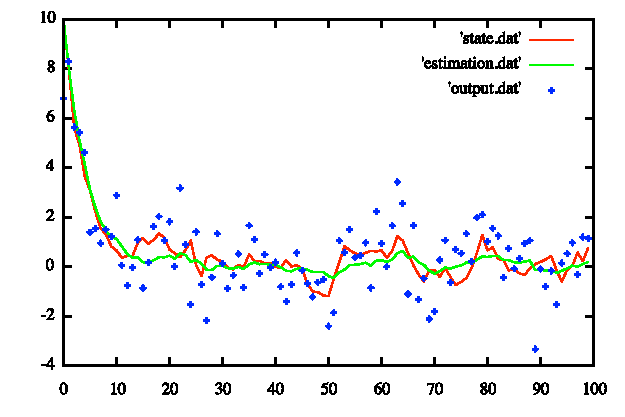
\includegraphics{ar_process}}
\end{ImageNoCaption}
\hypertarget{page2_sec3}{}\section{The CMakeList.txt}\label{page2_sec3}


\begin{DocInclude}\begin{verbatim}CMAKE_MINIMUM_REQUIRED(VERSION 2.6)

PROJECT(Van_Der_Pol)
ADD_DEFINITIONS(" -O3")

# GSL
SET(BFILT_LIB bfilt)

# Include et Link Directories

IF(APPLE)
  MESSAGE("-- Apple Configuration")
  INCLUDE_DIRECTORIES(
    /sw/include/
    )
ENDIF(APPLE)

# Executables and "stand-alone " librairies
ADD_EXECUTABLE (Van_Der_Pol
  van_der_pol.cpp
  example_3.cpp
  )

# Linkage
TARGET_LINK_LIBRARIES(Van_Der_Pol
  ${BFILT_LIB}     
  )
\end{verbatim}
\end{DocInclude}
 
\chapter{An Ornstien-Uhlenbeck process}
\label{page2}
\hypertarget{page2}{}
This example illustrate how to use BFilt for continuous-discrete filtering. Here the state is described by the following linear stochastic differential equation : \[ d \left ( \begin{array}{c} x \\ \dot{x} \\ \end{array} \right ) = \left ( \begin{array}{cc} 0 & 1 \\ -w_0^2 & -\gamma \\ \end{array} \right ) \left ( \begin{array}{c} x \\ \dot{x} \\ \end{array} \right ) dt + \left( \begin{array}{c} 0 \\ b \\ \end{array} \right ) dt + \left ( \begin{array}{c} 0 \\ g \\ \end{array} \right ) dW(t) \]

Where W(t) is a Wiener process,

$ w_0^2=16, \gamma = 2, b=8, g=2$ and the initials conditions $ X_0=(0,0) $ and $ R_0=diag[0,3]$.

The state $ X(t) = (x,\dot{x})(t)$ is then observed by the output $ Y_k \in \mathcal{R} $ : \[ Y_k = x(t_k) + V_k \]

at discrete time $ t_k $. The sampling period $ T_s = t_{k-1} - t_k = 0.2s $ and $ V_k \sim \mathcal{N}(0,0.001) $. In fact only the position is observed. First this model must be define as a sister class of linear time invariant continuous discrete models (\hyperlink{class_linear___c_d___model}{Linear\_\-CD\_\-Model}). 

\begin{DocInclude}\begin{verbatim}#ifndef __ORNSTEIN_UHL__
#define __ORNSTEIN_UHL__

#include <bfilt/gaussian_model.h>

class Ornstein_Uhlenbeck_Model : public Linear_CD_Model
{
public :
      double gamma;
      double w;
      double b;
      double g;
      Ornstein_Uhlenbeck_Model(void);


};

#endif
\end{verbatim}
\end{DocInclude}
 The \hyperlink{class_linear___c_d___model}{Linear\_\-CD\_\-Model} are implemented in the following form : \[ dX(t) = A X(t)dt + Bdt + C dW(t) \] \[ Y_k = H X(t_k) + h + V_k \] The constructor of Ornstein\_\-Uhlenbeck\_\-Model is then : 

\begin{DocInclude}\begin{verbatim}#include "ornstein_uhlenbeck.h"

Ornstein_Uhlenbeck_Model::Ornstein_Uhlenbeck_Model(void)
{
      // parameters
      w = 4.;
      gamma = 2.;
      b = 8.;
      g = 2.;

      // Matrices of the state equation
      A.resize(2,2);
      A(0,0) = 0.;
      A(0,1) = 1.;
      A(1,0) = - (w*w);
      A(1,1) = -gamma;
      
      
      B.resize(2);
      B(0) = 0;
      B(1) = b;

      C.resize(2,1);
      C(0,0)=0.;
      C(1,0)=g;

      // Matrices of the Observation equation
      H.resize(1,2);
      H(0,0) = 1.;
      H(0,1) = 0.;

      h.resize(2);
      h.zero();

      Qw.resize(1);
      Qw.identity();
      Qw*=0.01;

      Qv.resize(1);
      Qv(0,0) = 0.001;

      // Sampling period
      Ts = 0.2;

      // Initial conditions
      R0.resize(2);
      R0.zero();
      R0(0,0)=0.;
      R0(1,1)=3.;
      
      X0.resize(2);
      X0.zero();
            

}
\end{verbatim}
\end{DocInclude}
\hypertarget{page2_sec2}{}\section{The main program}\label{page2_sec2}
In the main program, the model will be first simulted with a specific simulator for \hyperlink{class_linear___c_d___model}{Linear\_\-CD\_\-Model} (\hyperlink{class_l_t_i___c_d___simulator}{LTI\_\-CD\_\-Simulator}). The simulated output sequence $ y_{0:N}$ is given to the input of the continuous-discrete kalman filter (\hyperlink{class_c_d___filter}{CD\_\-Filter}) to estimate the state trajectory $ \hat{X}_{0:k} $. First, all this objects are declared :

 

\begin{DocInclude}\begin{verbatim}int main(int argc, char **argv)
{
      Ornstein_Uhlenbeck_Model model; // The model

      LTI_CD_Simulator sim(&model);   // The simulator
      
      CD_Kalman  filter(&model);      // The Kalman filter      
\end{verbatim}
\end{DocInclude}


Then 10 second are simulated : 

\begin{DocInclude}\begin{verbatim}      sim.Simulate(10.);
\end{verbatim}
\end{DocInclude}
 The kalman filter is apply on the output sequence : 

\begin{DocInclude}\begin{verbatim}\end{verbatim}
\end{DocInclude}
 You can save the simulated sequences : 

\begin{DocInclude}\begin{verbatim}      sim.Save_Y("output.dat");
      sim.Save_X("state.dat");
\end{verbatim}
\end{DocInclude}


and the estimated state : 

\begin{DocInclude}\begin{verbatim}      filter.Save_X("estimation.dat");
\end{verbatim}
\end{DocInclude}


After compileing and execution, with Gnuplot you can plot : 

\begin{Code}\begin{verbatim}  plot 'state.dat' w l, 'estimation.dat' w l, 'output.dat'
\end{verbatim}
\end{Code}

 To obtain the following graph :  \begin{ImageNoCaption}\mbox{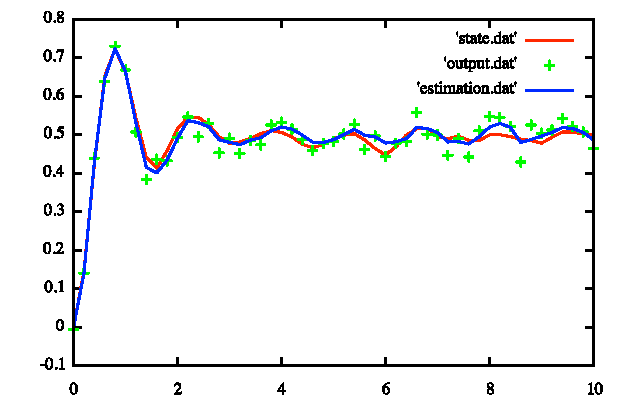
\includegraphics{ornstein}}
\end{ImageNoCaption}
\hypertarget{page2_sec3}{}\section{The CMakeList.txt}\label{page2_sec3}


\begin{DocInclude}\begin{verbatim}CMAKE_MINIMUM_REQUIRED(VERSION 2.6)

PROJECT(Van_Der_Pol)
ADD_DEFINITIONS(" -O3")

# GSL
SET(BFILT_LIB bfilt)

# Include et Link Directories

IF(APPLE)
  MESSAGE("-- Apple Configuration")
  INCLUDE_DIRECTORIES(
    /sw/include/
    )
ENDIF(APPLE)

# Executables and "stand-alone " librairies
ADD_EXECUTABLE (Van_Der_Pol
  van_der_pol.cpp
  example_3.cpp
  )

# Linkage
TARGET_LINK_LIBRARIES(Van_Der_Pol
  ${BFILT_LIB}     
  )
\end{verbatim}
\end{DocInclude}
 
\chapter{Van Der Pol oscillator}
\label{page_3}
\hypertarget{page_3}{}
This example on the Van der Pol oscillator shows how to use BFilt for non-linear continuous-discrete model. Here the van\_\-der\_\-pol class : \begin{Desc}
\item[]van\_\-der\_\-pol.h 

\begin{DocInclude}\begin{verbatim}#ifndef __VAN_DER_POL
#define __VAN_DER_POL


#include <bfilt/gaussian_model.h>


class Van_Der_Pol : public Continuous_Discrete_Model
{
public :
      double lambda;
      
      Van_Der_Pol(void);
      dcovector Drift_Function(const dcovector & X);
      dgematrix J_Drift_Function(const dcovector & X);
      dcovector Observation_Function(const dcovector& X);
      dgematrix J_Observation_Function(const dcovector & X);
      dgematrix Diffusion_Function(void);
};


#endif
\end{verbatim}
\end{DocInclude}
 van\_\-der\_\-pol.cpp 

\begin{DocInclude}\begin{verbatim}#include "van_der_pol.h"

Van_Der_Pol::Van_Der_Pol(void)
{
      lambda = 3.;

      Qw.resize(1);
      Qw(0,0)= 1.;
      Qv.resize(1);
      Qv(0,0)=0.1;
  
      X0.resize(2);
      X0(0) = 0.5;
      X0(1) = 0.5;
      R0.resize(2);
      R0.zero();
      R0(0,0)=0.;
      R0(1,1)=.1;
      Ts=.1;

}


dcovector Van_Der_Pol::Drift_Function(const dcovector & X)
{
      dcovector dX(X.l);

      dX(0) = X(1);
      dX(1) = lambda * (1. - X(0) * X(0)) * X(1) - X(0);

      return dX;
}

dgematrix Van_Der_Pol::J_Drift_Function(const dcovector & X)
{
      dgematrix F(X.l,X.l);

      F(0,0) = 0.;
      F(0,1) = 1.;
      F(1,0) = -2. * lambda * X(0) * X(1);
      F(1,1) = - lambda * X(0) * X(0);

      return F;
}
dcovector Van_Der_Pol::Observation_Function(const dcovector& X)
{
      dcovector Y(1);
      Y(0) = X(0);
      return Y;
}

dgematrix Van_Der_Pol::J_Observation_Function(const dcovector & X)
{
      dgematrix H(1,2);
      H(0,0) = 0.;
      H(0,1) = 1.;
      return H;
}
dgematrix Van_Der_Pol::Diffusion_Function(void)
{
      dgematrix G(2,1);
      G(0,0) = 0.;
      G(1,0) = 1.;

      return G;
}
\end{verbatim}
\end{DocInclude}
 The main program : 

\begin{DocInclude}\begin{verbatim}#include <bfilt/simulator.h>
#include <bfilt/extended_kalman_filter.h>
#include "van_der_pol.h"



int main(int argc, char **argv)
{
      Van_Der_Pol model;              // The model

      CD_Simulator sim(&model);   // The simulator
      
      CD_Extended_Kalman_Filter  filter(&model,THGL);      // The filter
      
      // Simulation 40 seconds
      sim.Simulate(40.);
        

      // Filtering from the simulated output sim.Y
      filter.Filtering(sim.Y);

      // Output Files for simulation
      sim.Save_Y("output.dat");
      sim.Save_X("state.dat");

      // Output File for filtering
      filter.Save_X("estimation.dat");
 
      return 0;
}
\end{verbatim}
\end{DocInclude}
 Results can be plotted (here with gnuplot):  \begin{ImageNoCaption}\mbox{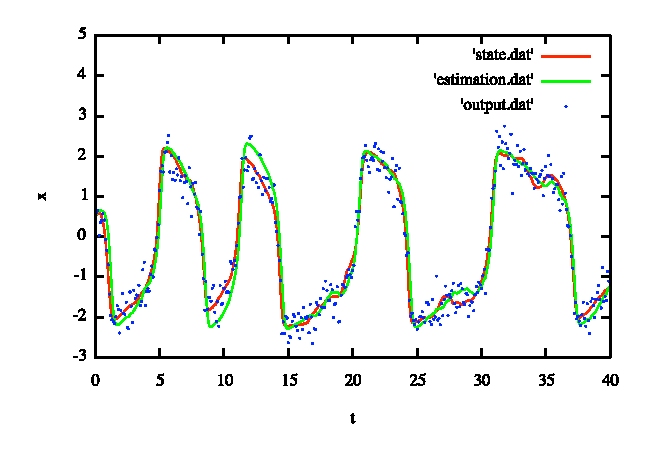
\includegraphics{van_der_pol}}
\end{ImageNoCaption}
 \end{Desc}

\chapter{Terrain navigation}
\label{page_4}
\hypertarget{page_4}{}
This example illustrate performances of particle filter to highly non-linear filter. The promblem here involves a plane whose the trajectory is a brownian motion. This aircraft measure the elevation. The measure of this elevation and an elevation map are then used to estimate the position of the plane.  \begin{ImageNoCaption}\mbox{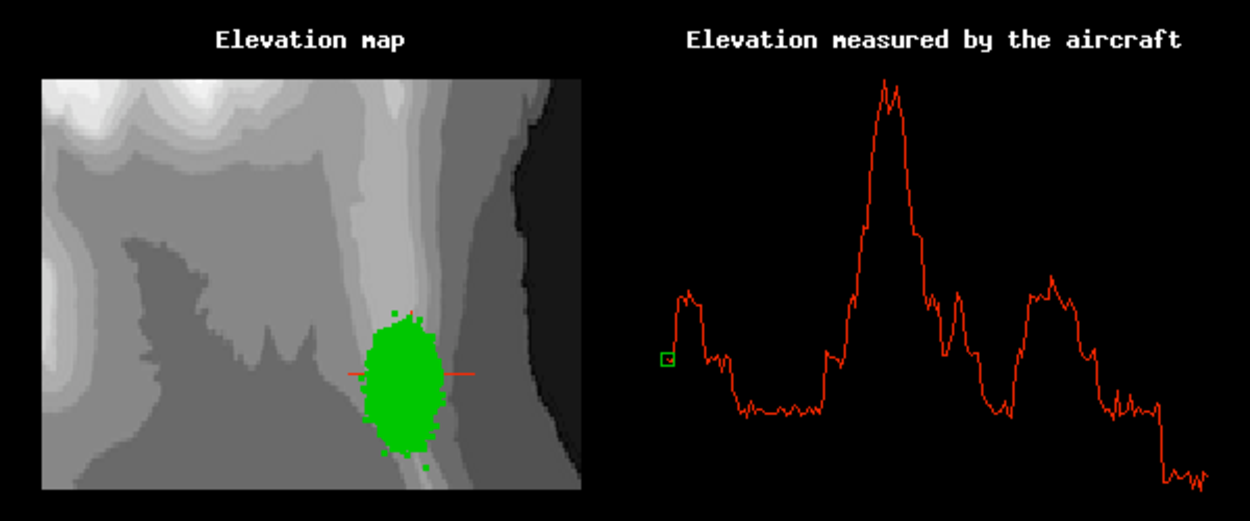
\includegraphics{plane}}
\end{ImageNoCaption}


plane.h 

\begin{DocInclude}\begin{verbatim}#ifndef __PLANE
#define __PLANE

#include <bfilt/gaussian_model.h>

class Plane : public Gaussian_Nonlinear_Model
{
      vector<double> Map;
      double xmin;
      double xmax;
      double ymin;
      double ymax;

      double sigv;
      double sigc;
public :
      Plane(const char *filename);

      dcovector State_Function(const dcovector &X, const dcovector &W);
      dcovector Observation_Function(const dcovector & X);
};


#endif
\end{verbatim}
\end{DocInclude}
 plane.cpp 

\begin{DocInclude}\begin{verbatim}#include "plane.h"

Plane::Plane(const char * filename)
{
      int x,y,z;
      ifstream file(filename);

      if(file)
            {
                              file>>xmax;
                              file>>ymin;
                              file>>z;
                              Map.push_back(z);

                  while(!file.eof())
                        {
                              file>>x;
                              file>>y;
                              file>>z;
                              Map.push_back(z);

                              if(x>xmax)
                                    xmax=x;
                              if(x<xmin)
                                    xmin=x;
                              if(y>ymax)
                                    ymax=y;
                              if(y<ymin)
                                    ymin=y;
                              
                        }
                  file.close();
            }
      else 
            {
                  cout<<"Plane :: error file"<<endl;
            }

      Qw.resize(2);
      Qw.identity();
      Qv.resize(1);
      Qv.identity();
      Qv*=5.;
      R0.resize(4);
      R0.zero();
      R0(0,0)=10.;
      R0(1,1)=10.;
      R0(2,2) = .001;
      R0(3,3) = 0.0001;
      X0.resize(4);
      X0(0)=120.;
      X0(1)=20.;
      X0(2)=1.5;
      X0(3)=2.35;


      sigv = .001;
      sigc = 0.03;
            
}

dcovector Plane::State_Function(const dcovector &X, const dcovector &W)
{
      dcovector U(4);

      U(0) = X(0) + X(2) * cos(X(3));
      U(1) = X(1) + X(2) * sin(X(3));
      U(2) = X(2) + sigv * W(0);
      U(3) = X(3) + sigc * W(1);
      if (U(0)>xmax)
            {
                  U(0)=xmax;
                  U(3)=3.14-U(3);
            }
      if (U(1)>ymax)
            {
                  U(1)=ymax;
                  U(3)=-U(3);
            }
      if (U(0)<xmin)
            {
                  U(0)=xmin;
                  U(3)=3.14-U(3);
            }
      if (U(1)<ymin)
            {
                  U(1)=ymin;
                  U(3)=-U(3);
            }

      return U;
}
dcovector Plane::Observation_Function(const dcovector & X)
{
      int x = (int)(X(0));
      int y = (int)(X(1));
      int j= (xmax+1)*y + x;
      dcovector Y(1);
      Y(0)=Map[j];
      return Y;
}

\end{verbatim}
\end{DocInclude}
 The main program : 

\begin{DocInclude}\begin{verbatim}#include <bfilt/simulator.h>
#include <bfilt/sisr_filter.h>
#include "plane.h"

// This example illustrate performances of particle filter to highly non-linear 
// filter. The promblem here involves a plane whose the trajectory is a brownian
// motion. This aircraft measure the elevation. The measure of this elevation and 
// an elevation map are then used to estimate the position of the plane.
int main(int argc, char **argv)
{
      int k;
      int i;
      int j;
      vector<Weighted_Sample> cloud;

      ofstream file_c("../data/cloud.dat"); // To save the cloud
      ofstream file_s("../data/state.dat"); // To save the state

      Plane       plane("../data/map_2.dat");       // The plane model
      G_Simulator sim(&plane);                    // To simulate a this model
      
      Bootstrap_Filter filter(100000,&plane);       // A bootstrap filter to estimate the position

      sim.Simulate(150);                     // simulation of 250 samples

      sim.Save_Y("../data/output.dat");     // save the output

      // Here Init() and Update methods are used
      // for filtering because we want to get the cloud 
      // at each step and save it in cloud.dat

      filter.Init();                      // Initialization of the boostrap filter
      
      for (k=0; k<sim.Y.size(); k++)
            {

                  cloud=filter.CloudGet();              // The current cloud is return

                  for(i=0; i<cloud.size(); i++)         // and here it is saved
                        {
                              for(j=0; j<cloud[i].Value.l; j++)
                                    file_c<<cloud[i].Value(j)<<" ";
                              file_c<<endl;
                        }

                  for (j=0; j<sim.X[k].l; j++)       // The state is also saved
                        file_s<<sim.X[k](j)<<" ";
                  file_s<<endl<<endl<<endl;
                  file_c<<endl<<endl;

                  if( filter.Update(sim.Y[k]))              // The filter is then update with a new observation
                        filter.Init();
            }
      file_c.close();
      file_s.close();

      return 0;
}
\end{verbatim}
\end{DocInclude}
 
\chapter{Class Index}
\section{Class Hierarchy}
This inheritance list is sorted roughly, but not completely, alphabetically:\begin{CompactList}
\item \contentsline{section}{Filter}{\pageref{class_filter}}{}
\begin{CompactList}
\item \contentsline{section}{CD\_\-Filter}{\pageref{class_c_d___filter}}{}
\begin{CompactList}
\item \contentsline{section}{CD\_\-Extended\_\-Kalman\_\-Filter}{\pageref{class_c_d___extended___kalman___filter}}{}
\item \contentsline{section}{CD\_\-Kalman}{\pageref{class_c_d___kalman}}{}
\item \contentsline{section}{LL\_\-Filter}{\pageref{class_l_l___filter}}{}
\item \contentsline{section}{THGL\_\-Filter}{\pageref{class_t_h_g_l___filter}}{}
\end{CompactList}
\item \contentsline{section}{GA\_\-Filter}{\pageref{class_g_a___filter}}{}
\begin{CompactList}
\item \contentsline{section}{DD\_\-Kalman}{\pageref{class_d_d___kalman}}{}
\item \contentsline{section}{Extended\_\-Kalman\_\-Filter}{\pageref{class_extended___kalman___filter}}{}
\item \contentsline{section}{Unscented\_\-Kalman\_\-Filter}{\pageref{class_unscented___kalman___filter}}{}
\end{CompactList}
\item \contentsline{section}{SISR\_\-Filter}{\pageref{class_s_i_s_r___filter}}{}
\begin{CompactList}
\item \contentsline{section}{Bootstrap\_\-Filter}{\pageref{class_bootstrap___filter}}{}
\item \contentsline{section}{CD\_\-Bootstrap\_\-Filter}{\pageref{class_c_d___bootstrap___filter}}{}
\item \contentsline{section}{OptSISR\_\-Filter}{\pageref{class_opt_s_i_s_r___filter}}{}
\end{CompactList}
\end{CompactList}
\item \contentsline{section}{Model}{\pageref{class_model}}{}
\begin{CompactList}
\item \contentsline{section}{Discrete\_\-Observed\_\-Model}{\pageref{class_discrete___observed___model}}{}
\begin{CompactList}
\item \contentsline{section}{Continuous\_\-Discrete\_\-Model}{\pageref{class_continuous___discrete___model}}{}
\begin{CompactList}
\item \contentsline{section}{Linear\_\-CD\_\-Model}{\pageref{class_linear___c_d___model}}{}
\end{CompactList}
\item \contentsline{section}{Gaussian\_\-Nonlinear\_\-Model}{\pageref{class_gaussian___nonlinear___model}}{}
\begin{CompactList}
\item \contentsline{section}{Discrete\_\-Approximation\_\-CD\_\-Model}{\pageref{class_discrete___approximation___c_d___model}}{}
\begin{CompactList}
\item \contentsline{section}{Euler\_\-CD\_\-Model}{\pageref{class_euler___c_d___model}}{}
\item \contentsline{section}{Heun\_\-CD\_\-Model}{\pageref{class_heun___c_d___model}}{}
\item \contentsline{section}{Ozaki\_\-CD\_\-Model}{\pageref{class_ozaki___c_d___model}}{}
\item \contentsline{section}{SRK4\_\-CD\_\-Model}{\pageref{class_s_r_k4___c_d___model}}{}
\end{CompactList}
\item \contentsline{section}{Gaussian\_\-Linear\_\-Model}{\pageref{class_gaussian___linear___model}}{}
\end{CompactList}
\end{CompactList}
\end{CompactList}
\item \contentsline{section}{SI\_\-Sampler}{\pageref{class_s_i___sampler}}{}
\begin{CompactList}
\item \contentsline{section}{Bootstrap\_\-Sampler}{\pageref{class_bootstrap___sampler}}{}
\item \contentsline{section}{Optimal\_\-Sampler}{\pageref{class_optimal___sampler}}{}
\end{CompactList}
\item \contentsline{section}{Simulator}{\pageref{class_simulator}}{}
\begin{CompactList}
\item \contentsline{section}{CD\_\-Simulator}{\pageref{class_c_d___simulator}}{}
\begin{CompactList}
\item \contentsline{section}{CD\_\-Simulator\_\-WT}{\pageref{class_c_d___simulator___w_t}}{}
\item \contentsline{section}{LTI\_\-CD\_\-Simulator}{\pageref{class_l_t_i___c_d___simulator}}{}
\begin{CompactList}
\item \contentsline{section}{LTI\_\-CD\_\-Simulator\_\-WT}{\pageref{class_l_t_i___c_d___simulator___w_t}}{}
\end{CompactList}
\end{CompactList}
\item \contentsline{section}{Opt\_\-Simulator}{\pageref{class_opt___simulator}}{}
\begin{CompactList}
\item \contentsline{section}{G\_\-Simulator}{\pageref{class_g___simulator}}{}
\begin{CompactList}
\item \contentsline{section}{G\_\-Simulator\_\-WT}{\pageref{class_g___simulator___w_t}}{}
\end{CompactList}
\end{CompactList}
\end{CompactList}
\item \contentsline{section}{Weighted\_\-Sample}{\pageref{class_weighted___sample}}{}
\end{CompactList}

\chapter{Class Index}
\section{Class List}
Here are the classes, structs, unions and interfaces with brief descriptions:\begin{CompactList}
\item\contentsline{section}{\hyperlink{class_bootstrap___filter}{Bootstrap\_\-Filter} }{\pageref{class_bootstrap___filter}}{}
\item\contentsline{section}{\hyperlink{class_bootstrap___sampler}{Bootstrap\_\-Sampler} (This sampler use the transition as importance density )}{\pageref{class_bootstrap___sampler}}{}
\item\contentsline{section}{\hyperlink{class_c_d___bootstrap___filter}{CD\_\-Bootstrap\_\-Filter} }{\pageref{class_c_d___bootstrap___filter}}{}
\item\contentsline{section}{\hyperlink{class_c_d___extended___kalman___filter}{CD\_\-Extended\_\-Kalman\_\-Filter} }{\pageref{class_c_d___extended___kalman___filter}}{}
\item\contentsline{section}{\hyperlink{class_c_d___filter}{CD\_\-Filter} (Abstract class of continuous-discrete filters )}{\pageref{class_c_d___filter}}{}
\item\contentsline{section}{\hyperlink{class_c_d___kalman}{CD\_\-Kalman} (The continuous-discrete kalman filter )}{\pageref{class_c_d___kalman}}{}
\item\contentsline{section}{\hyperlink{class_c_d___simulator}{CD\_\-Simulator} }{\pageref{class_c_d___simulator}}{}
\item\contentsline{section}{\hyperlink{class_c_d___simulator___w_t}{CD\_\-Simulator\_\-WT} }{\pageref{class_c_d___simulator___w_t}}{}
\item\contentsline{section}{\hyperlink{class_continuous___discrete___model}{Continuous\_\-Discrete\_\-Model} (Continuous Discrete \hyperlink{class_model}{Model}: The continuous state : $ dX(t) = F(X)dt + G()*d\beta $ The discrete Observation $ Yk = H (X(tk)) + Vk $ )}{\pageref{class_continuous___discrete___model}}{}
\item\contentsline{section}{\hyperlink{class_d_d___kalman}{DD\_\-Kalman} (The discrete-discrete kalman filter )}{\pageref{class_d_d___kalman}}{}
\item\contentsline{section}{\hyperlink{class_discrete___approximation___c_d___model}{Discrete\_\-Approximation\_\-CD\_\-Model} (Continuous state equation is discretly approximate by X(tk) = f'(X(tk-1),Wk) )}{\pageref{class_discrete___approximation___c_d___model}}{}
\item\contentsline{section}{\hyperlink{class_discrete___observed___model}{Discrete\_\-Observed\_\-Model} (Class of discretely observed model )}{\pageref{class_discrete___observed___model}}{}
\item\contentsline{section}{\hyperlink{class_euler___c_d___model}{Euler\_\-CD\_\-Model} (Continuous discret model: the state SDE is discretly approximate by an Euler method )}{\pageref{class_euler___c_d___model}}{}
\item\contentsline{section}{\hyperlink{class_extended___kalman___filter}{Extended\_\-Kalman\_\-Filter} }{\pageref{class_extended___kalman___filter}}{}
\item\contentsline{section}{\hyperlink{class_filter}{Filter} (Abstract class of all filters )}{\pageref{class_filter}}{}
\item\contentsline{section}{\hyperlink{class_g___simulator}{G\_\-Simulator} }{\pageref{class_g___simulator}}{}
\item\contentsline{section}{\hyperlink{class_g___simulator___w_t}{G\_\-Simulator\_\-WT} }{\pageref{class_g___simulator___w_t}}{}
\item\contentsline{section}{\hyperlink{class_g_a___filter}{GA\_\-Filter} (Abstract class of Gaussian Approximation filters )}{\pageref{class_g_a___filter}}{}
\item\contentsline{section}{\hyperlink{class_gaussian___linear___model}{Gaussian\_\-Linear\_\-Model} (Gaussian Linear \hyperlink{class_model}{Model} : )}{\pageref{class_gaussian___linear___model}}{}
\item\contentsline{section}{\hyperlink{class_gaussian___nonlinear___model}{Gaussian\_\-Nonlinear\_\-Model} (Gaussian Nonlinear \hyperlink{class_model}{Model} The state : X(k) = F (Xk-1, Wk) The Observation Y(k) = H (X(k)) + V )}{\pageref{class_gaussian___nonlinear___model}}{}
\item\contentsline{section}{\hyperlink{class_heun___c_d___model}{Heun\_\-CD\_\-Model} (Continuous discret model: the state SDE is discretly approximate by an Sstochastic Heun method )}{\pageref{class_heun___c_d___model}}{}
\item\contentsline{section}{\hyperlink{class_linear___c_d___model}{Linear\_\-CD\_\-Model} (Linear continuous discrete model class of the form dx = AX dt + Bdt + CdW Y\_\-k = HX(t\_\-k) + h + V\_\-k )}{\pageref{class_linear___c_d___model}}{}
\item\contentsline{section}{\hyperlink{class_l_l___filter}{LL\_\-Filter} }{\pageref{class_l_l___filter}}{}
\item\contentsline{section}{\hyperlink{class_l_t_i___c_d___simulator}{LTI\_\-CD\_\-Simulator} }{\pageref{class_l_t_i___c_d___simulator}}{}
\item\contentsline{section}{\hyperlink{class_l_t_i___c_d___simulator___w_t}{LTI\_\-CD\_\-Simulator\_\-WT} }{\pageref{class_l_t_i___c_d___simulator___w_t}}{}
\item\contentsline{section}{\hyperlink{class_model}{Model} (The class of time varying-models )}{\pageref{class_model}}{}
\item\contentsline{section}{\hyperlink{class_opt___simulator}{Opt\_\-Simulator} }{\pageref{class_opt___simulator}}{}
\item\contentsline{section}{\hyperlink{class_optimal___sampler}{Optimal\_\-Sampler} (This sampler use the optimal importance density )}{\pageref{class_optimal___sampler}}{}
\item\contentsline{section}{\hyperlink{class_opt_s_i_s_r___filter}{OptSISR\_\-Filter} }{\pageref{class_opt_s_i_s_r___filter}}{}
\item\contentsline{section}{\hyperlink{class_ozaki___c_d___model}{Ozaki\_\-CD\_\-Model} (Continuous discret model: the state SDE is discretly approximate by Ozaki method )}{\pageref{class_ozaki___c_d___model}}{}
\item\contentsline{section}{\hyperlink{class_s_i___sampler}{SI\_\-Sampler} (Sequential importance sampler used for sisr filter (bootstrap,optimal ...) )}{\pageref{class_s_i___sampler}}{}
\item\contentsline{section}{\hyperlink{class_simulator}{Simulator} }{\pageref{class_simulator}}{}
\item\contentsline{section}{\hyperlink{class_s_i_s_r___filter}{SISR\_\-Filter} }{\pageref{class_s_i_s_r___filter}}{}
\item\contentsline{section}{\hyperlink{class_s_r_k4___c_d___model}{SRK4\_\-CD\_\-Model} (Continuous discret model: the state SDE is discretly approximate by an Sstochastic runge kutta method )}{\pageref{class_s_r_k4___c_d___model}}{}
\item\contentsline{section}{\hyperlink{class_t_h_g_l___filter}{THGL\_\-Filter} }{\pageref{class_t_h_g_l___filter}}{}
\item\contentsline{section}{\hyperlink{class_unscented___kalman___filter}{Unscented\_\-Kalman\_\-Filter} (The Discrete Unscented Kalman \hyperlink{class_filter}{Filter} (UKF) )}{\pageref{class_unscented___kalman___filter}}{}
\item\contentsline{section}{\hyperlink{class_weighted___sample}{Weighted\_\-Sample} }{\pageref{class_weighted___sample}}{}
\end{CompactList}

\chapter{Class Documentation}
\hypertarget{class_bootstrap___filter}{
\section{Bootstrap\_\-Filter Class Reference}
\label{class_bootstrap___filter}\index{Bootstrap\_\-Filter@{Bootstrap\_\-Filter}}
}
{\tt \#include $<$sisr\_\-filter.h$>$}

Inheritance diagram for Bootstrap\_\-Filter:\nopagebreak
\begin{figure}[H]
\begin{center}
\leavevmode
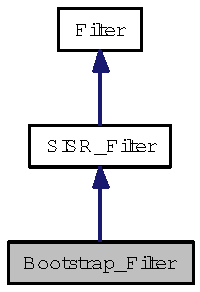
\includegraphics[width=66pt]{class_bootstrap___filter__inherit__graph}
\end{center}
\end{figure}
\subsection*{Public Member Functions}
\begin{CompactItemize}
\item 
\hyperlink{class_bootstrap___filter_bdebb4e715920561261919a08c0adbe6}{Bootstrap\_\-Filter} (void)
\item 
\hyperlink{class_bootstrap___filter_95cab25094e2488a9c417a40fc7d4afc}{$\sim$Bootstrap\_\-Filter} (void)
\item 
\hyperlink{class_bootstrap___filter_616427f3269bb6b4e0b23e66e4b748b7}{Bootstrap\_\-Filter} (const int \&Ns, \hyperlink{class_simulator}{Simulator} $\ast$s)
\item 
\hyperlink{class_bootstrap___filter_b6cd1f6d02e6fb00ba41a7b10b03228a}{Bootstrap\_\-Filter} (const int \&Ns, \hyperlink{class_gaussian___nonlinear___model}{Gaussian\_\-Nonlinear\_\-Model} $\ast$m)
\end{CompactItemize}
\subsection*{Private Attributes}
\begin{CompactItemize}
\item 
\hyperlink{class_simulator}{Simulator} $\ast$ \hyperlink{class_bootstrap___filter_5b4cfb2f584027060dff43bc967cb77c}{sim}
\end{CompactItemize}


\subsection{Constructor \& Destructor Documentation}
\hypertarget{class_bootstrap___filter_bdebb4e715920561261919a08c0adbe6}{
\index{Bootstrap\_\-Filter@{Bootstrap\_\-Filter}!Bootstrap\_\-Filter@{Bootstrap\_\-Filter}}
\index{Bootstrap\_\-Filter@{Bootstrap\_\-Filter}!Bootstrap_Filter@{Bootstrap\_\-Filter}}
\subsubsection[{Bootstrap\_\-Filter}]{\setlength{\rightskip}{0pt plus 5cm}Bootstrap\_\-Filter::Bootstrap\_\-Filter (void)}}
\label{class_bootstrap___filter_bdebb4e715920561261919a08c0adbe6}


\hypertarget{class_bootstrap___filter_95cab25094e2488a9c417a40fc7d4afc}{
\index{Bootstrap\_\-Filter@{Bootstrap\_\-Filter}!$\sim$Bootstrap\_\-Filter@{$\sim$Bootstrap\_\-Filter}}
\index{$\sim$Bootstrap\_\-Filter@{$\sim$Bootstrap\_\-Filter}!Bootstrap_Filter@{Bootstrap\_\-Filter}}
\subsubsection[{$\sim$Bootstrap\_\-Filter}]{\setlength{\rightskip}{0pt plus 5cm}Bootstrap\_\-Filter::$\sim$Bootstrap\_\-Filter (void)}}
\label{class_bootstrap___filter_95cab25094e2488a9c417a40fc7d4afc}


\hypertarget{class_bootstrap___filter_616427f3269bb6b4e0b23e66e4b748b7}{
\index{Bootstrap\_\-Filter@{Bootstrap\_\-Filter}!Bootstrap\_\-Filter@{Bootstrap\_\-Filter}}
\index{Bootstrap\_\-Filter@{Bootstrap\_\-Filter}!Bootstrap_Filter@{Bootstrap\_\-Filter}}
\subsubsection[{Bootstrap\_\-Filter}]{\setlength{\rightskip}{0pt plus 5cm}Bootstrap\_\-Filter::Bootstrap\_\-Filter (const int \& {\em Ns}, \/  {\bf Simulator} $\ast$ {\em s})}}
\label{class_bootstrap___filter_616427f3269bb6b4e0b23e66e4b748b7}


\hypertarget{class_bootstrap___filter_b6cd1f6d02e6fb00ba41a7b10b03228a}{
\index{Bootstrap\_\-Filter@{Bootstrap\_\-Filter}!Bootstrap\_\-Filter@{Bootstrap\_\-Filter}}
\index{Bootstrap\_\-Filter@{Bootstrap\_\-Filter}!Bootstrap_Filter@{Bootstrap\_\-Filter}}
\subsubsection[{Bootstrap\_\-Filter}]{\setlength{\rightskip}{0pt plus 5cm}Bootstrap\_\-Filter::Bootstrap\_\-Filter (const int \& {\em Ns}, \/  {\bf Gaussian\_\-Nonlinear\_\-Model} $\ast$ {\em m})}}
\label{class_bootstrap___filter_b6cd1f6d02e6fb00ba41a7b10b03228a}




\subsection{Member Data Documentation}
\hypertarget{class_bootstrap___filter_5b4cfb2f584027060dff43bc967cb77c}{
\index{Bootstrap\_\-Filter@{Bootstrap\_\-Filter}!sim@{sim}}
\index{sim@{sim}!Bootstrap_Filter@{Bootstrap\_\-Filter}}
\subsubsection[{sim}]{\setlength{\rightskip}{0pt plus 5cm}{\bf Simulator}$\ast$ {\bf Bootstrap\_\-Filter::sim}\hspace{0.3cm}{\tt  \mbox{[}private\mbox{]}}}}
\label{class_bootstrap___filter_5b4cfb2f584027060dff43bc967cb77c}



\hypertarget{class_bootstrap___sampler}{
\section{Bootstrap\_\-Sampler Class Reference}
\label{class_bootstrap___sampler}\index{Bootstrap\_\-Sampler@{Bootstrap\_\-Sampler}}
}
This sampler use the transition as importance density.  


{\tt \#include $<$sisr\_\-filter.h$>$}

Inheritance diagram for Bootstrap\_\-Sampler:\nopagebreak
\begin{figure}[H]
\begin{center}
\leavevmode
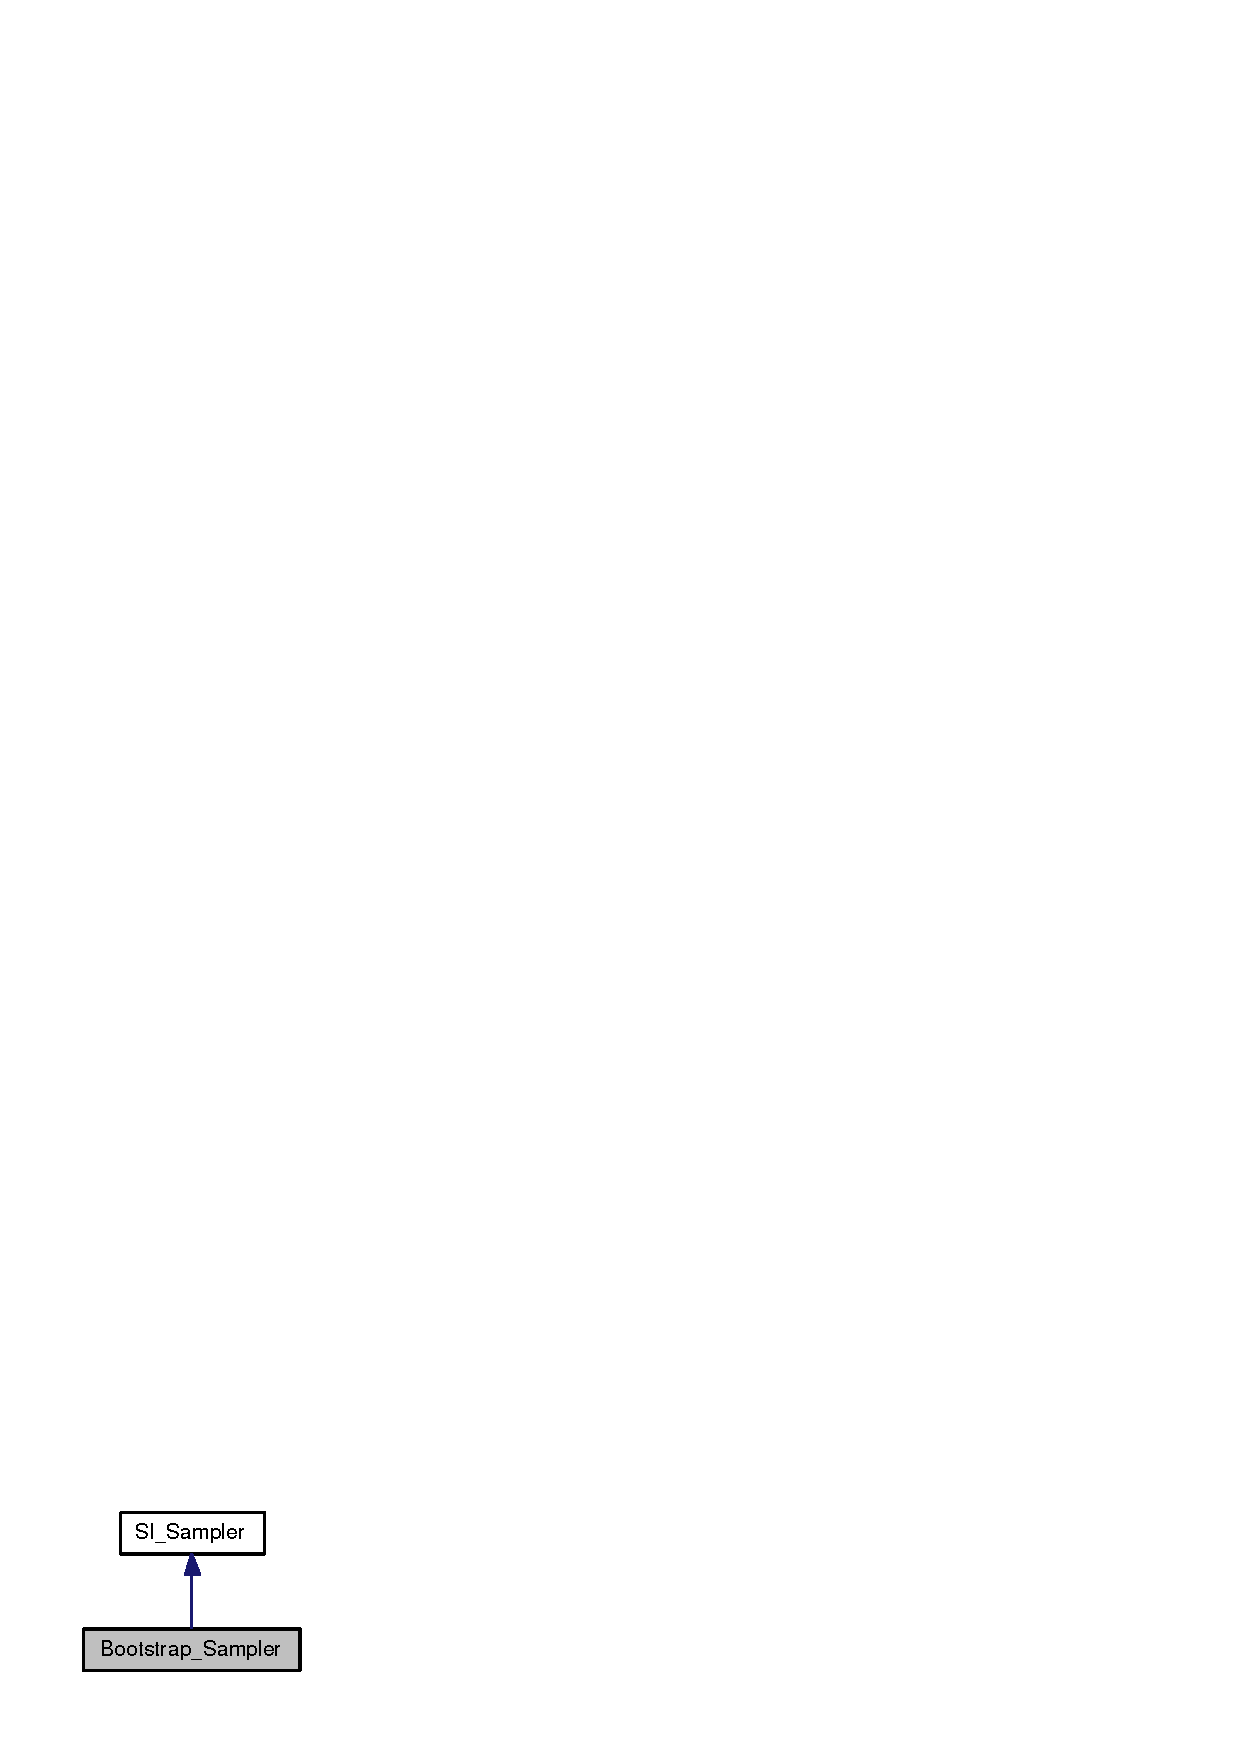
\includegraphics[width=74pt]{class_bootstrap___sampler__inherit__graph}
\end{center}
\end{figure}
\subsection*{Public Member Functions}
\begin{CompactItemize}
\item 
\hyperlink{class_bootstrap___sampler_bf03144ecc96fdc63267d050ed91e71b}{Bootstrap\_\-Sampler} (void)
\item 
\hyperlink{class_bootstrap___sampler_484a287a562f6f3801d5547cfff0b757}{Bootstrap\_\-Sampler} (\hyperlink{class_simulator}{Simulator} $\ast$m)
\item 
vector$<$ \hyperlink{class_weighted___sample}{Weighted\_\-Sample} $>$ \hyperlink{class_bootstrap___sampler_e36eb9258b052c41e075b350960d21a3}{DrawInitCloud} (const int \&NbSample)
\begin{CompactList}\small\item\em draw a set of possible init state \item\end{CompactList}\item 
vector$<$ \hyperlink{class_weighted___sample}{Weighted\_\-Sample} $>$ \hyperlink{class_bootstrap___sampler_a826164a46c257f5a95ba0b4eba7ee83}{Draw} (const dcovector \&Y\_\-k, const vector$<$ \hyperlink{class_weighted___sample}{Weighted\_\-Sample} $>$ \&X\_\-km1)
\begin{CompactList}\small\item\em Draw a set of samples from the importance density Xk given Y0:k X0:k-1. \item\end{CompactList}\item 
long double \hyperlink{class_bootstrap___sampler_22ca201b958c0c873cfdbd1d545140dc}{Weight} (vector$<$ \hyperlink{class_weighted___sample}{Weighted\_\-Sample} $>$ \&cloud, const dcovector \&Y\_\-k, const vector$<$ \hyperlink{class_weighted___sample}{Weighted\_\-Sample} $>$ \&X\_\-k)
\begin{CompactList}\small\item\em Modify the weights of cloud for the weighting step in the sisr. \item\end{CompactList}\end{CompactItemize}


\subsection{Detailed Description}
This sampler use the transition as importance density. 



\subsection{Constructor \& Destructor Documentation}
\hypertarget{class_bootstrap___sampler_bf03144ecc96fdc63267d050ed91e71b}{
\index{Bootstrap\_\-Sampler@{Bootstrap\_\-Sampler}!Bootstrap\_\-Sampler@{Bootstrap\_\-Sampler}}
\index{Bootstrap\_\-Sampler@{Bootstrap\_\-Sampler}!Bootstrap_Sampler@{Bootstrap\_\-Sampler}}
\subsubsection[{Bootstrap\_\-Sampler}]{\setlength{\rightskip}{0pt plus 5cm}Bootstrap\_\-Sampler::Bootstrap\_\-Sampler (void)}}
\label{class_bootstrap___sampler_bf03144ecc96fdc63267d050ed91e71b}


\hypertarget{class_bootstrap___sampler_484a287a562f6f3801d5547cfff0b757}{
\index{Bootstrap\_\-Sampler@{Bootstrap\_\-Sampler}!Bootstrap\_\-Sampler@{Bootstrap\_\-Sampler}}
\index{Bootstrap\_\-Sampler@{Bootstrap\_\-Sampler}!Bootstrap_Sampler@{Bootstrap\_\-Sampler}}
\subsubsection[{Bootstrap\_\-Sampler}]{\setlength{\rightskip}{0pt plus 5cm}Bootstrap\_\-Sampler::Bootstrap\_\-Sampler ({\bf Simulator} $\ast$ {\em m})}}
\label{class_bootstrap___sampler_484a287a562f6f3801d5547cfff0b757}




\subsection{Member Function Documentation}
\hypertarget{class_bootstrap___sampler_a826164a46c257f5a95ba0b4eba7ee83}{
\index{Bootstrap\_\-Sampler@{Bootstrap\_\-Sampler}!Draw@{Draw}}
\index{Draw@{Draw}!Bootstrap_Sampler@{Bootstrap\_\-Sampler}}
\subsubsection[{Draw}]{\setlength{\rightskip}{0pt plus 5cm}vector$<${\bf Weighted\_\-Sample} $>$ Bootstrap\_\-Sampler::Draw (const dcovector \& {\em Y\_\-k}, \/  const vector$<$ {\bf Weighted\_\-Sample} $>$ \& {\em X\_\-km1})\hspace{0.3cm}{\tt  \mbox{[}virtual\mbox{]}}}}
\label{class_bootstrap___sampler_a826164a46c257f5a95ba0b4eba7ee83}


Draw a set of samples from the importance density Xk given Y0:k X0:k-1. 

\begin{Desc}
\item[Parameters:]
\begin{description}
\item[{\em Y\_\-k}]The observation from 0 to k \item[{\em X\_\-km1}]The cloud from 0 to km1\end{description}
\end{Desc}
\begin{Desc}
\item[Returns:]A cloud representing the importance density q(Xk$|$Y0:k,X0:k-1) \end{Desc}


Implements \hyperlink{class_s_i___sampler_62bf57181aeb5981426a71a7bf01c3e9}{SI\_\-Sampler}.\hypertarget{class_bootstrap___sampler_e36eb9258b052c41e075b350960d21a3}{
\index{Bootstrap\_\-Sampler@{Bootstrap\_\-Sampler}!DrawInitCloud@{DrawInitCloud}}
\index{DrawInitCloud@{DrawInitCloud}!Bootstrap_Sampler@{Bootstrap\_\-Sampler}}
\subsubsection[{DrawInitCloud}]{\setlength{\rightskip}{0pt plus 5cm}vector$<${\bf Weighted\_\-Sample} $>$ Bootstrap\_\-Sampler::DrawInitCloud (const int \& {\em NbSample})\hspace{0.3cm}{\tt  \mbox{[}virtual\mbox{]}}}}
\label{class_bootstrap___sampler_e36eb9258b052c41e075b350960d21a3}


draw a set of possible init state 

\begin{Desc}
\item[Parameters:]
\begin{description}
\item[{\em NbSample}]Number of sample\end{description}
\end{Desc}
\begin{Desc}
\item[Returns:]A set of weighted samples \end{Desc}


Implements \hyperlink{class_s_i___sampler_3fbedf1ce189168da5608861d5a3289e}{SI\_\-Sampler}.\hypertarget{class_bootstrap___sampler_22ca201b958c0c873cfdbd1d545140dc}{
\index{Bootstrap\_\-Sampler@{Bootstrap\_\-Sampler}!Weight@{Weight}}
\index{Weight@{Weight}!Bootstrap_Sampler@{Bootstrap\_\-Sampler}}
\subsubsection[{Weight}]{\setlength{\rightskip}{0pt plus 5cm}long double Bootstrap\_\-Sampler::Weight (vector$<$ {\bf Weighted\_\-Sample} $>$ \& {\em cloud}, \/  const dcovector \& {\em Y\_\-k}, \/  const vector$<$ {\bf Weighted\_\-Sample} $>$ \& {\em X\_\-km1})\hspace{0.3cm}{\tt  \mbox{[}virtual\mbox{]}}}}
\label{class_bootstrap___sampler_22ca201b958c0c873cfdbd1d545140dc}


Modify the weights of cloud for the weighting step in the sisr. 

\begin{Desc}
\item[Parameters:]
\begin{description}
\item[{\em cloud}]The curent coud at k \item[{\em Y\_\-k}]The observation at k \item[{\em X\_\-km1}]the cloud from at km1\end{description}
\end{Desc}
\begin{Desc}
\item[Returns:]The sum of the weights \end{Desc}


Implements \hyperlink{class_s_i___sampler_5c3a3547060d91febd3ef61969756ab6}{SI\_\-Sampler}.
\hypertarget{class_c_d___bootstrap___filter}{
\section{CD\_\-Bootstrap\_\-Filter Class Reference}
\label{class_c_d___bootstrap___filter}\index{CD\_\-Bootstrap\_\-Filter@{CD\_\-Bootstrap\_\-Filter}}
}
{\tt \#include $<$sisr\_\-filter.h$>$}

Inheritance diagram for CD\_\-Bootstrap\_\-Filter:\nopagebreak
\begin{figure}[H]
\begin{center}
\leavevmode
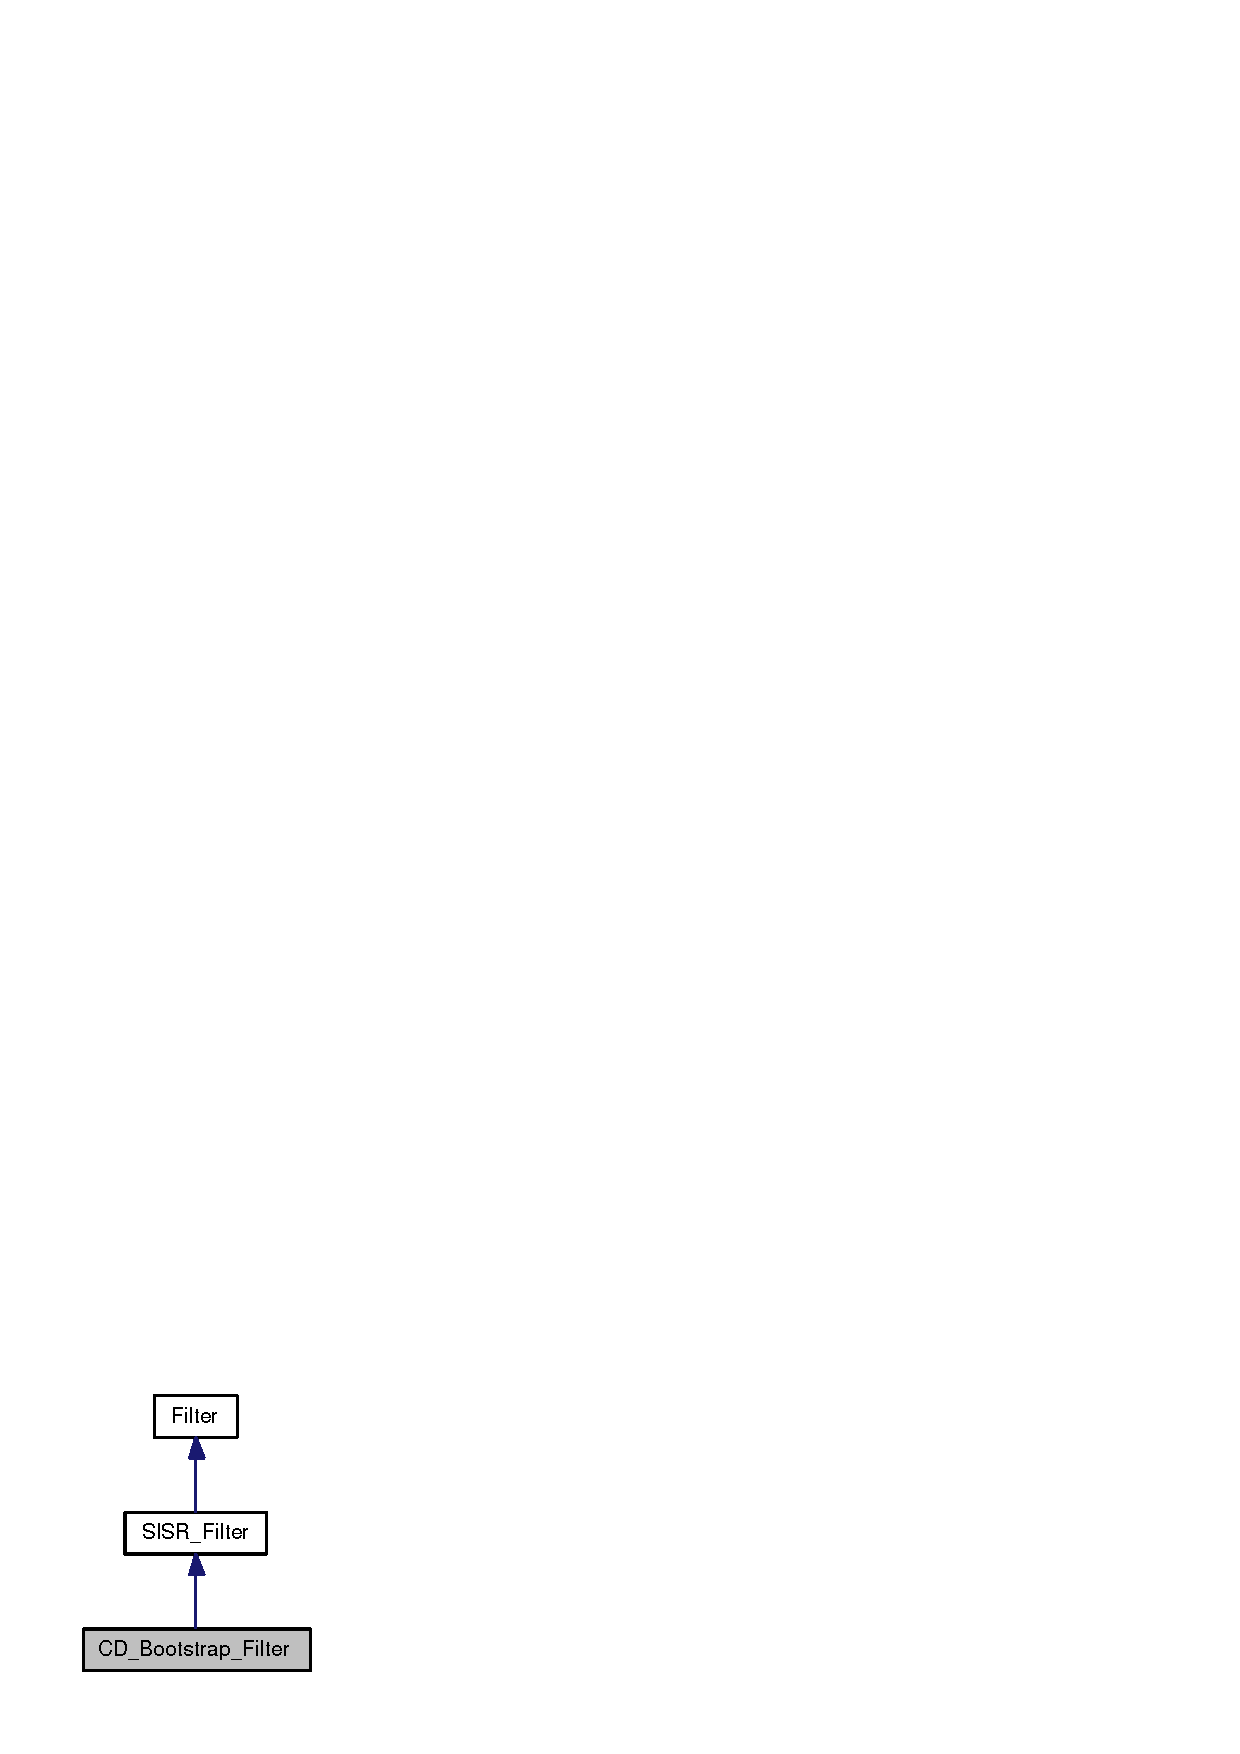
\includegraphics[width=76pt]{class_c_d___bootstrap___filter__inherit__graph}
\end{center}
\end{figure}
\subsection*{Public Member Functions}
\begin{CompactItemize}
\item 
\hyperlink{class_c_d___bootstrap___filter_5a6857c370a2573d8e3bcb4eab10eef2}{CD\_\-Bootstrap\_\-Filter} (void)
\item 
\hyperlink{class_c_d___bootstrap___filter_13d757890e69283429b4a17893b639bc}{$\sim$CD\_\-Bootstrap\_\-Filter} (void)
\item 
\hyperlink{class_c_d___bootstrap___filter_b57c5fe3037188132aadb91d883da2dd}{CD\_\-Bootstrap\_\-Filter} (const int \&Ns, \hyperlink{class_c_d___simulator}{CD\_\-Simulator} $\ast$s)
\item 
\hyperlink{class_c_d___bootstrap___filter_bff15b578b01eb0b7cb4d71f044123a2}{CD\_\-Bootstrap\_\-Filter} (const int \&Ns, \hyperlink{class_continuous___discrete___model}{Continuous\_\-Discrete\_\-Model} $\ast$m)
\item 
\hyperlink{class_c_d___bootstrap___filter_2b404414afe25a0a62abf45d22e34a8c}{CD\_\-Bootstrap\_\-Filter} (const int \&Ns, \hyperlink{class_linear___c_d___model}{Linear\_\-CD\_\-Model} $\ast$m)
\item 
virtual int \hyperlink{class_c_d___bootstrap___filter_eb203b8cdeb51133a232dce5763ed153}{Save\_\-X} (const char $\ast$filename)
\end{CompactItemize}
\subsection*{Private Attributes}
\begin{CompactItemize}
\item 
\hyperlink{class_c_d___simulator}{CD\_\-Simulator} $\ast$ \hyperlink{class_c_d___bootstrap___filter_ac76dfed8e2d0d994558b50a4fe242f7}{sim}
\end{CompactItemize}


\subsection{Constructor \& Destructor Documentation}
\hypertarget{class_c_d___bootstrap___filter_5a6857c370a2573d8e3bcb4eab10eef2}{
\index{CD\_\-Bootstrap\_\-Filter@{CD\_\-Bootstrap\_\-Filter}!CD\_\-Bootstrap\_\-Filter@{CD\_\-Bootstrap\_\-Filter}}
\index{CD\_\-Bootstrap\_\-Filter@{CD\_\-Bootstrap\_\-Filter}!CD_Bootstrap_Filter@{CD\_\-Bootstrap\_\-Filter}}
\subsubsection[{CD\_\-Bootstrap\_\-Filter}]{\setlength{\rightskip}{0pt plus 5cm}CD\_\-Bootstrap\_\-Filter::CD\_\-Bootstrap\_\-Filter (void)}}
\label{class_c_d___bootstrap___filter_5a6857c370a2573d8e3bcb4eab10eef2}


\hypertarget{class_c_d___bootstrap___filter_13d757890e69283429b4a17893b639bc}{
\index{CD\_\-Bootstrap\_\-Filter@{CD\_\-Bootstrap\_\-Filter}!$\sim$CD\_\-Bootstrap\_\-Filter@{$\sim$CD\_\-Bootstrap\_\-Filter}}
\index{$\sim$CD\_\-Bootstrap\_\-Filter@{$\sim$CD\_\-Bootstrap\_\-Filter}!CD_Bootstrap_Filter@{CD\_\-Bootstrap\_\-Filter}}
\subsubsection[{$\sim$CD\_\-Bootstrap\_\-Filter}]{\setlength{\rightskip}{0pt plus 5cm}CD\_\-Bootstrap\_\-Filter::$\sim$CD\_\-Bootstrap\_\-Filter (void)}}
\label{class_c_d___bootstrap___filter_13d757890e69283429b4a17893b639bc}


\hypertarget{class_c_d___bootstrap___filter_b57c5fe3037188132aadb91d883da2dd}{
\index{CD\_\-Bootstrap\_\-Filter@{CD\_\-Bootstrap\_\-Filter}!CD\_\-Bootstrap\_\-Filter@{CD\_\-Bootstrap\_\-Filter}}
\index{CD\_\-Bootstrap\_\-Filter@{CD\_\-Bootstrap\_\-Filter}!CD_Bootstrap_Filter@{CD\_\-Bootstrap\_\-Filter}}
\subsubsection[{CD\_\-Bootstrap\_\-Filter}]{\setlength{\rightskip}{0pt plus 5cm}CD\_\-Bootstrap\_\-Filter::CD\_\-Bootstrap\_\-Filter (const int \& {\em Ns}, \/  {\bf CD\_\-Simulator} $\ast$ {\em s})}}
\label{class_c_d___bootstrap___filter_b57c5fe3037188132aadb91d883da2dd}


\hypertarget{class_c_d___bootstrap___filter_bff15b578b01eb0b7cb4d71f044123a2}{
\index{CD\_\-Bootstrap\_\-Filter@{CD\_\-Bootstrap\_\-Filter}!CD\_\-Bootstrap\_\-Filter@{CD\_\-Bootstrap\_\-Filter}}
\index{CD\_\-Bootstrap\_\-Filter@{CD\_\-Bootstrap\_\-Filter}!CD_Bootstrap_Filter@{CD\_\-Bootstrap\_\-Filter}}
\subsubsection[{CD\_\-Bootstrap\_\-Filter}]{\setlength{\rightskip}{0pt plus 5cm}CD\_\-Bootstrap\_\-Filter::CD\_\-Bootstrap\_\-Filter (const int \& {\em Ns}, \/  {\bf Continuous\_\-Discrete\_\-Model} $\ast$ {\em m})}}
\label{class_c_d___bootstrap___filter_bff15b578b01eb0b7cb4d71f044123a2}


\hypertarget{class_c_d___bootstrap___filter_2b404414afe25a0a62abf45d22e34a8c}{
\index{CD\_\-Bootstrap\_\-Filter@{CD\_\-Bootstrap\_\-Filter}!CD\_\-Bootstrap\_\-Filter@{CD\_\-Bootstrap\_\-Filter}}
\index{CD\_\-Bootstrap\_\-Filter@{CD\_\-Bootstrap\_\-Filter}!CD_Bootstrap_Filter@{CD\_\-Bootstrap\_\-Filter}}
\subsubsection[{CD\_\-Bootstrap\_\-Filter}]{\setlength{\rightskip}{0pt plus 5cm}CD\_\-Bootstrap\_\-Filter::CD\_\-Bootstrap\_\-Filter (const int \& {\em Ns}, \/  {\bf Linear\_\-CD\_\-Model} $\ast$ {\em m})}}
\label{class_c_d___bootstrap___filter_2b404414afe25a0a62abf45d22e34a8c}




\subsection{Member Function Documentation}
\hypertarget{class_c_d___bootstrap___filter_eb203b8cdeb51133a232dce5763ed153}{
\index{CD\_\-Bootstrap\_\-Filter@{CD\_\-Bootstrap\_\-Filter}!Save\_\-X@{Save\_\-X}}
\index{Save\_\-X@{Save\_\-X}!CD_Bootstrap_Filter@{CD\_\-Bootstrap\_\-Filter}}
\subsubsection[{Save\_\-X}]{\setlength{\rightskip}{0pt plus 5cm}virtual int CD\_\-Bootstrap\_\-Filter::Save\_\-X (const char $\ast$ {\em filename})\hspace{0.3cm}{\tt  \mbox{[}virtual\mbox{]}}}}
\label{class_c_d___bootstrap___filter_eb203b8cdeb51133a232dce5763ed153}


Save the estimation $ \{ \hat{X}_{k|k} ,k=0,...N \} $

\begin{Desc}
\item[Parameters:]
\begin{description}
\item[{\em filename}]\end{description}
\end{Desc}
\begin{Desc}
\item[Returns:]0 if everything is ok \end{Desc}


Reimplemented from \hyperlink{class_filter_0b7aad4b130b176f423b7f1c0c30a887}{Filter}.

\subsection{Member Data Documentation}
\hypertarget{class_c_d___bootstrap___filter_ac76dfed8e2d0d994558b50a4fe242f7}{
\index{CD\_\-Bootstrap\_\-Filter@{CD\_\-Bootstrap\_\-Filter}!sim@{sim}}
\index{sim@{sim}!CD_Bootstrap_Filter@{CD\_\-Bootstrap\_\-Filter}}
\subsubsection[{sim}]{\setlength{\rightskip}{0pt plus 5cm}{\bf CD\_\-Simulator}$\ast$ {\bf CD\_\-Bootstrap\_\-Filter::sim}\hspace{0.3cm}{\tt  \mbox{[}private\mbox{]}}}}
\label{class_c_d___bootstrap___filter_ac76dfed8e2d0d994558b50a4fe242f7}



\hypertarget{class_c_d___extended___kalman___filter}{
\section{CD\_\-Extended\_\-Kalman\_\-Filter Class Reference}
\label{class_c_d___extended___kalman___filter}\index{CD\_\-Extended\_\-Kalman\_\-Filter@{CD\_\-Extended\_\-Kalman\_\-Filter}}
}
{\tt \#include $<$extended\_\-kalman\_\-filter.h$>$}

Inheritance diagram for CD\_\-Extended\_\-Kalman\_\-Filter:\nopagebreak
\begin{figure}[H]
\begin{center}
\leavevmode
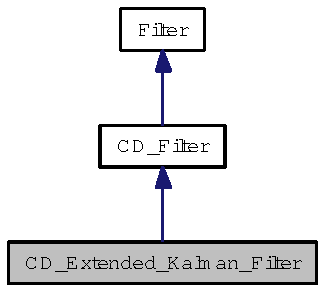
\includegraphics[width=96pt]{class_c_d___extended___kalman___filter__inherit__graph}
\end{center}
\end{figure}
\subsection*{Public Member Functions}
\begin{CompactItemize}
\item 
\hyperlink{class_c_d___extended___kalman___filter_a513c87055e01494c950391047fe8e78}{CD\_\-Extended\_\-Kalman\_\-Filter} (void)
\item 
\hyperlink{class_c_d___extended___kalman___filter_01743a0e2ac32830a65da4dc7885cc20}{CD\_\-Extended\_\-Kalman\_\-Filter} (\hyperlink{class_continuous___discrete___model}{Continuous\_\-Discrete\_\-Model} $\ast$m, const int \&sh=RK4)
\end{CompactItemize}
\subsection*{Public Attributes}
\begin{CompactItemize}
\item 
int \hyperlink{class_c_d___extended___kalman___filter_20c7448afdc652603781e4da3385e2b3}{Scheme}
\end{CompactItemize}
\subsection*{Protected Member Functions}
\begin{CompactItemize}
\item 
int \hyperlink{class_c_d___extended___kalman___filter_7cfd2bf966970f44f4e1480ed3852b69}{\_\-update} (const dcovector \&Y)
\item 
void \hyperlink{class_c_d___extended___kalman___filter_e11771d2cea027b53e17091e817e59bd}{\_\-thgl\_\-\_\-prediction} (dcovector \&\hyperlink{class_c_d___filter_1388124f777df49de87fa59058535cde}{M}, dgematrix \&P)
\item 
void \hyperlink{class_c_d___extended___kalman___filter_64fda06630749c6d5936fd7257690c68}{\_\-euler\_\-prediction} (dcovector \&\hyperlink{class_c_d___filter_1388124f777df49de87fa59058535cde}{M}, dgematrix \&P)
\item 
void \hyperlink{class_c_d___extended___kalman___filter_79f174e2ff2bb51ada2d1cee3240fbb1}{\_\-rk4\_\-\_\-\_\-prediction} (dcovector \&\hyperlink{class_c_d___filter_1388124f777df49de87fa59058535cde}{M}, dgematrix \&P)
\item 
void \hyperlink{class_c_d___extended___kalman___filter_f67b43de36333a88e233bb6c51d15ab7}{\_\-heun\_\-\_\-prediction} (dcovector \&\hyperlink{class_c_d___filter_1388124f777df49de87fa59058535cde}{M}, dgematrix \&P)
\item 
void \hyperlink{class_c_d___extended___kalman___filter_aff3514a20d714c817780fa1871f4a9d}{\_\-rk4\_\-\_\-\_\-prediction\_\-FM} (dcovector \&\hyperlink{class_c_d___filter_1388124f777df49de87fa59058535cde}{M}, dgematrix \&P)
\end{CompactItemize}


\subsection{Constructor \& Destructor Documentation}
\hypertarget{class_c_d___extended___kalman___filter_a513c87055e01494c950391047fe8e78}{
\index{CD\_\-Extended\_\-Kalman\_\-Filter@{CD\_\-Extended\_\-Kalman\_\-Filter}!CD\_\-Extended\_\-Kalman\_\-Filter@{CD\_\-Extended\_\-Kalman\_\-Filter}}
\index{CD\_\-Extended\_\-Kalman\_\-Filter@{CD\_\-Extended\_\-Kalman\_\-Filter}!CD_Extended_Kalman_Filter@{CD\_\-Extended\_\-Kalman\_\-Filter}}
\subsubsection[{CD\_\-Extended\_\-Kalman\_\-Filter}]{\setlength{\rightskip}{0pt plus 5cm}CD\_\-Extended\_\-Kalman\_\-Filter::CD\_\-Extended\_\-Kalman\_\-Filter (void)}}
\label{class_c_d___extended___kalman___filter_a513c87055e01494c950391047fe8e78}


\hypertarget{class_c_d___extended___kalman___filter_01743a0e2ac32830a65da4dc7885cc20}{
\index{CD\_\-Extended\_\-Kalman\_\-Filter@{CD\_\-Extended\_\-Kalman\_\-Filter}!CD\_\-Extended\_\-Kalman\_\-Filter@{CD\_\-Extended\_\-Kalman\_\-Filter}}
\index{CD\_\-Extended\_\-Kalman\_\-Filter@{CD\_\-Extended\_\-Kalman\_\-Filter}!CD_Extended_Kalman_Filter@{CD\_\-Extended\_\-Kalman\_\-Filter}}
\subsubsection[{CD\_\-Extended\_\-Kalman\_\-Filter}]{\setlength{\rightskip}{0pt plus 5cm}CD\_\-Extended\_\-Kalman\_\-Filter::CD\_\-Extended\_\-Kalman\_\-Filter ({\bf Continuous\_\-Discrete\_\-Model} $\ast$ {\em m}, \/  const int \& {\em sh} = {\tt RK4})}}
\label{class_c_d___extended___kalman___filter_01743a0e2ac32830a65da4dc7885cc20}




\subsection{Member Function Documentation}
\hypertarget{class_c_d___extended___kalman___filter_64fda06630749c6d5936fd7257690c68}{
\index{CD\_\-Extended\_\-Kalman\_\-Filter@{CD\_\-Extended\_\-Kalman\_\-Filter}!\_\-euler\_\-prediction@{\_\-euler\_\-prediction}}
\index{\_\-euler\_\-prediction@{\_\-euler\_\-prediction}!CD_Extended_Kalman_Filter@{CD\_\-Extended\_\-Kalman\_\-Filter}}
\subsubsection[{\_\-euler\_\-prediction}]{\setlength{\rightskip}{0pt plus 5cm}void CD\_\-Extended\_\-Kalman\_\-Filter::\_\-euler\_\-prediction (dcovector \& {\em M}, \/  dgematrix \& {\em P})\hspace{0.3cm}{\tt  \mbox{[}protected\mbox{]}}}}
\label{class_c_d___extended___kalman___filter_64fda06630749c6d5936fd7257690c68}


\hypertarget{class_c_d___extended___kalman___filter_f67b43de36333a88e233bb6c51d15ab7}{
\index{CD\_\-Extended\_\-Kalman\_\-Filter@{CD\_\-Extended\_\-Kalman\_\-Filter}!\_\-heun\_\-\_\-prediction@{\_\-heun\_\-\_\-prediction}}
\index{\_\-heun\_\-\_\-prediction@{\_\-heun\_\-\_\-prediction}!CD_Extended_Kalman_Filter@{CD\_\-Extended\_\-Kalman\_\-Filter}}
\subsubsection[{\_\-heun\_\-\_\-prediction}]{\setlength{\rightskip}{0pt plus 5cm}void CD\_\-Extended\_\-Kalman\_\-Filter::\_\-heun\_\-\_\-prediction (dcovector \& {\em M}, \/  dgematrix \& {\em P})\hspace{0.3cm}{\tt  \mbox{[}protected\mbox{]}}}}
\label{class_c_d___extended___kalman___filter_f67b43de36333a88e233bb6c51d15ab7}


\hypertarget{class_c_d___extended___kalman___filter_79f174e2ff2bb51ada2d1cee3240fbb1}{
\index{CD\_\-Extended\_\-Kalman\_\-Filter@{CD\_\-Extended\_\-Kalman\_\-Filter}!\_\-rk4\_\-\_\-\_\-prediction@{\_\-rk4\_\-\_\-\_\-prediction}}
\index{\_\-rk4\_\-\_\-\_\-prediction@{\_\-rk4\_\-\_\-\_\-prediction}!CD_Extended_Kalman_Filter@{CD\_\-Extended\_\-Kalman\_\-Filter}}
\subsubsection[{\_\-rk4\_\-\_\-\_\-prediction}]{\setlength{\rightskip}{0pt plus 5cm}void CD\_\-Extended\_\-Kalman\_\-Filter::\_\-rk4\_\-\_\-\_\-prediction (dcovector \& {\em M}, \/  dgematrix \& {\em P})\hspace{0.3cm}{\tt  \mbox{[}protected\mbox{]}}}}
\label{class_c_d___extended___kalman___filter_79f174e2ff2bb51ada2d1cee3240fbb1}


\hypertarget{class_c_d___extended___kalman___filter_aff3514a20d714c817780fa1871f4a9d}{
\index{CD\_\-Extended\_\-Kalman\_\-Filter@{CD\_\-Extended\_\-Kalman\_\-Filter}!\_\-rk4\_\-\_\-\_\-prediction\_\-FM@{\_\-rk4\_\-\_\-\_\-prediction\_\-FM}}
\index{\_\-rk4\_\-\_\-\_\-prediction\_\-FM@{\_\-rk4\_\-\_\-\_\-prediction\_\-FM}!CD_Extended_Kalman_Filter@{CD\_\-Extended\_\-Kalman\_\-Filter}}
\subsubsection[{\_\-rk4\_\-\_\-\_\-prediction\_\-FM}]{\setlength{\rightskip}{0pt plus 5cm}void CD\_\-Extended\_\-Kalman\_\-Filter::\_\-rk4\_\-\_\-\_\-prediction\_\-FM (dcovector \& {\em M}, \/  dgematrix \& {\em P})\hspace{0.3cm}{\tt  \mbox{[}protected\mbox{]}}}}
\label{class_c_d___extended___kalman___filter_aff3514a20d714c817780fa1871f4a9d}


\hypertarget{class_c_d___extended___kalman___filter_e11771d2cea027b53e17091e817e59bd}{
\index{CD\_\-Extended\_\-Kalman\_\-Filter@{CD\_\-Extended\_\-Kalman\_\-Filter}!\_\-thgl\_\-\_\-prediction@{\_\-thgl\_\-\_\-prediction}}
\index{\_\-thgl\_\-\_\-prediction@{\_\-thgl\_\-\_\-prediction}!CD_Extended_Kalman_Filter@{CD\_\-Extended\_\-Kalman\_\-Filter}}
\subsubsection[{\_\-thgl\_\-\_\-prediction}]{\setlength{\rightskip}{0pt plus 5cm}void CD\_\-Extended\_\-Kalman\_\-Filter::\_\-thgl\_\-\_\-prediction (dcovector \& {\em M}, \/  dgematrix \& {\em P})\hspace{0.3cm}{\tt  \mbox{[}protected\mbox{]}}}}
\label{class_c_d___extended___kalman___filter_e11771d2cea027b53e17091e817e59bd}


\hypertarget{class_c_d___extended___kalman___filter_7cfd2bf966970f44f4e1480ed3852b69}{
\index{CD\_\-Extended\_\-Kalman\_\-Filter@{CD\_\-Extended\_\-Kalman\_\-Filter}!\_\-update@{\_\-update}}
\index{\_\-update@{\_\-update}!CD_Extended_Kalman_Filter@{CD\_\-Extended\_\-Kalman\_\-Filter}}
\subsubsection[{\_\-update}]{\setlength{\rightskip}{0pt plus 5cm}int CD\_\-Extended\_\-Kalman\_\-Filter::\_\-update (const dcovector \& {\em Y})\hspace{0.3cm}{\tt  \mbox{[}protected, virtual\mbox{]}}}}
\label{class_c_d___extended___kalman___filter_7cfd2bf966970f44f4e1480ed3852b69}


Specific update for each filter

\begin{Desc}
\item[Parameters:]
\begin{description}
\item[{\em Y}]The observed sample\end{description}
\end{Desc}
\begin{Desc}
\item[Returns:]0 if no problem \end{Desc}


Implements \hyperlink{class_filter_20ecd17fed3b8f11a76c960fe5e7144b}{Filter}.

\subsection{Member Data Documentation}
\hypertarget{class_c_d___extended___kalman___filter_20c7448afdc652603781e4da3385e2b3}{
\index{CD\_\-Extended\_\-Kalman\_\-Filter@{CD\_\-Extended\_\-Kalman\_\-Filter}!Scheme@{Scheme}}
\index{Scheme@{Scheme}!CD_Extended_Kalman_Filter@{CD\_\-Extended\_\-Kalman\_\-Filter}}
\subsubsection[{Scheme}]{\setlength{\rightskip}{0pt plus 5cm}int {\bf CD\_\-Extended\_\-Kalman\_\-Filter::Scheme}}}
\label{class_c_d___extended___kalman___filter_20c7448afdc652603781e4da3385e2b3}



\hypertarget{class_c_d___filter}{
\section{CD\_\-Filter Class Reference}
\label{class_c_d___filter}\index{CD\_\-Filter@{CD\_\-Filter}}
}
Abstract class of continuous-discrete filters.  


{\tt \#include $<$filter.h$>$}

Inheritance diagram for CD\_\-Filter:\nopagebreak
\begin{figure}[H]
\begin{center}
\leavevmode
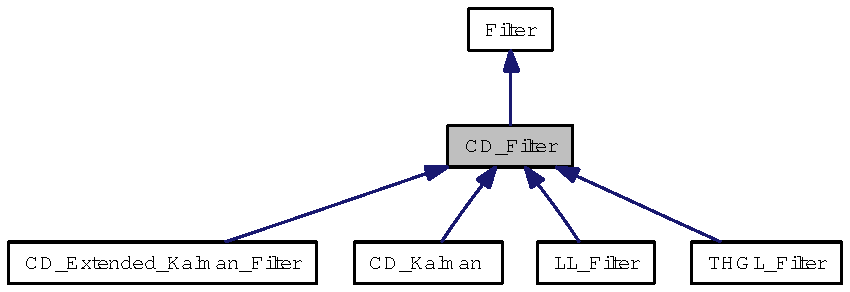
\includegraphics[width=400pt]{class_c_d___filter__inherit__graph}
\end{center}
\end{figure}
\subsection*{Public Member Functions}
\begin{CompactItemize}
\item 
\hyperlink{class_c_d___filter_b73ba4ee4ba0e1aaec09c8e88b8a4995}{CD\_\-Filter} (void)
\begin{CompactList}\small\item\em A constructor. \item\end{CompactList}\item 
\hyperlink{class_c_d___filter_b567ec6efd08a2f8bb33f3288c730346}{CD\_\-Filter} (\hyperlink{class_continuous___discrete___model}{Continuous\_\-Discrete\_\-Model} $\ast$m)
\item 
int \hyperlink{class_c_d___filter_b304de0cc156193c9e938188c1092188}{Save\_\-X} (const char $\ast$filename)
\item 
dcovector \hyperlink{class_c_d___filter_f5c2b82877e5cdad1e0cc782374809b0}{Expected\_\-Get} (void)
\end{CompactItemize}
\subsection*{Public Attributes}
\begin{CompactItemize}
\item 
dcovector \hyperlink{class_c_d___filter_1388124f777df49de87fa59058535cde}{M}
\begin{CompactList}\small\item\em The current mean $ \hat{X}_{k|k}=E[X_k |Y_{0:k}] $. \item\end{CompactList}\item 
dgematrix \hyperlink{class_c_d___filter_7a359404418fc49bf7a038ac27cc579b}{R}
\begin{CompactList}\small\item\em The current covariance $ \hat{P}_{k|k}=E[(X_k-\hat{X}_{k|k})(X_k-\hat{X}_{k|k})] $. \item\end{CompactList}\item 
dcovector \hyperlink{class_c_d___filter_a72ca0f05fe1359cf61ec5db0e1a3282}{Xp}
\begin{CompactList}\small\item\em The prediction $ \hat{X}_{k-1|k}=E[X_{k-1} |Y_{0:k}] $. \item\end{CompactList}\item 
dgematrix \hyperlink{class_c_d___filter_76bc9c00c330ffaa2815f073158353f3}{Rp}
\begin{CompactList}\small\item\em The prediction covariance $ \hat{P}_{k-1|k}=E[(X_k-\hat{X}_{k-1|k})(X_k-\hat{X}_{k-1|k}) ] $. \item\end{CompactList}\end{CompactItemize}
\subsection*{Protected Member Functions}
\begin{CompactItemize}
\item 
int \hyperlink{class_c_d___filter_789c745e24ee5534d22455dff70a93b3}{\_\-init} (void)
\end{CompactItemize}


\subsection{Detailed Description}
Abstract class of continuous-discrete filters. 

For continusous-discrete models (\hyperlink{class_continuous___discrete___model}{Continuous\_\-Discrete\_\-Model}), these filters approximate the probability density of the state transition $ p_{X(t_k)|X(t_{k-1})} $ and the probability of the observation $ p_{Y_k|X(t_k)} $ by gaussian densities. The approximation is exact in the case of linear continous-discrete models (\hyperlink{class_linear___c_d___model}{Linear\_\-CD\_\-Model}) and lead to the continuous-discrete Kalman \hyperlink{class_filter}{Filter} (\hyperlink{class_c_d___kalman}{CD\_\-Kalman}). For other non-linear models (\hyperlink{class_continuous___discrete___model}{Continuous\_\-Discrete\_\-Model}) Local linearization filter (\hyperlink{class_l_l___filter}{LL\_\-Filter}) or continous-discrete \hyperlink{class_filter}{Filter} EKF (\hyperlink{class_c_d___extended___kalman___filter}{CD\_\-Extended\_\-Kalman\_\-Filter}) can be used. 

\subsection{Constructor \& Destructor Documentation}
\hypertarget{class_c_d___filter_b73ba4ee4ba0e1aaec09c8e88b8a4995}{
\index{CD\_\-Filter@{CD\_\-Filter}!CD\_\-Filter@{CD\_\-Filter}}
\index{CD\_\-Filter@{CD\_\-Filter}!CD_Filter@{CD\_\-Filter}}
\subsubsection[{CD\_\-Filter}]{\setlength{\rightskip}{0pt plus 5cm}CD\_\-Filter::CD\_\-Filter (void)}}
\label{class_c_d___filter_b73ba4ee4ba0e1aaec09c8e88b8a4995}


A constructor. 

\hypertarget{class_c_d___filter_b567ec6efd08a2f8bb33f3288c730346}{
\index{CD\_\-Filter@{CD\_\-Filter}!CD\_\-Filter@{CD\_\-Filter}}
\index{CD\_\-Filter@{CD\_\-Filter}!CD_Filter@{CD\_\-Filter}}
\subsubsection[{CD\_\-Filter}]{\setlength{\rightskip}{0pt plus 5cm}CD\_\-Filter::CD\_\-Filter ({\bf Continuous\_\-Discrete\_\-Model} $\ast$ {\em m})}}
\label{class_c_d___filter_b567ec6efd08a2f8bb33f3288c730346}


A constructor

\begin{Desc}
\item[Parameters:]
\begin{description}
\item[{\em m}]A discrete-discrete gaussian non-linear model \end{description}
\end{Desc}


\subsection{Member Function Documentation}
\hypertarget{class_c_d___filter_789c745e24ee5534d22455dff70a93b3}{
\index{CD\_\-Filter@{CD\_\-Filter}!\_\-init@{\_\-init}}
\index{\_\-init@{\_\-init}!CD_Filter@{CD\_\-Filter}}
\subsubsection[{\_\-init}]{\setlength{\rightskip}{0pt plus 5cm}int CD\_\-Filter::\_\-init (void)\hspace{0.3cm}{\tt  \mbox{[}protected, virtual\mbox{]}}}}
\label{class_c_d___filter_789c745e24ee5534d22455dff70a93b3}


Specific init for each filter

\begin{Desc}
\item[Parameters:]
\begin{description}
\item[{\em Y}]The observed sample\end{description}
\end{Desc}
\begin{Desc}
\item[Returns:]0 if no problem \end{Desc}


Implements \hyperlink{class_filter_f46a456184971270ca36733d937f14fb}{Filter}.\hypertarget{class_c_d___filter_f5c2b82877e5cdad1e0cc782374809b0}{
\index{CD\_\-Filter@{CD\_\-Filter}!Expected\_\-Get@{Expected\_\-Get}}
\index{Expected\_\-Get@{Expected\_\-Get}!CD_Filter@{CD\_\-Filter}}
\subsubsection[{Expected\_\-Get}]{\setlength{\rightskip}{0pt plus 5cm}dcovector CD\_\-Filter::Expected\_\-Get (void)\hspace{0.3cm}{\tt  \mbox{[}virtual\mbox{]}}}}
\label{class_c_d___filter_f5c2b82877e5cdad1e0cc782374809b0}


Get the current estimation $ \hat{X}_{k|k} $

\begin{Desc}
\item[Returns:]$ \hat{X}_{k|k} $ \end{Desc}


Implements \hyperlink{class_filter_f6e41ec8ada47571291b31a259858cdc}{Filter}.\hypertarget{class_c_d___filter_b304de0cc156193c9e938188c1092188}{
\index{CD\_\-Filter@{CD\_\-Filter}!Save\_\-X@{Save\_\-X}}
\index{Save\_\-X@{Save\_\-X}!CD_Filter@{CD\_\-Filter}}
\subsubsection[{Save\_\-X}]{\setlength{\rightskip}{0pt plus 5cm}int CD\_\-Filter::Save\_\-X (const char $\ast$ {\em filename})\hspace{0.3cm}{\tt  \mbox{[}virtual\mbox{]}}}}
\label{class_c_d___filter_b304de0cc156193c9e938188c1092188}


Save the estimation $ \{ \hat{X}_{k|k} ,k=0,...N \} $

\begin{Desc}
\item[Parameters:]
\begin{description}
\item[{\em filename}]\end{description}
\end{Desc}
\begin{Desc}
\item[Returns:]0 if everything is ok \end{Desc}


Reimplemented from \hyperlink{class_filter_0b7aad4b130b176f423b7f1c0c30a887}{Filter}.

\subsection{Member Data Documentation}
\hypertarget{class_c_d___filter_1388124f777df49de87fa59058535cde}{
\index{CD\_\-Filter@{CD\_\-Filter}!M@{M}}
\index{M@{M}!CD_Filter@{CD\_\-Filter}}
\subsubsection[{M}]{\setlength{\rightskip}{0pt plus 5cm}dcovector {\bf CD\_\-Filter::M}}}
\label{class_c_d___filter_1388124f777df49de87fa59058535cde}


The current mean $ \hat{X}_{k|k}=E[X_k |Y_{0:k}] $. 

\hypertarget{class_c_d___filter_7a359404418fc49bf7a038ac27cc579b}{
\index{CD\_\-Filter@{CD\_\-Filter}!R@{R}}
\index{R@{R}!CD_Filter@{CD\_\-Filter}}
\subsubsection[{R}]{\setlength{\rightskip}{0pt plus 5cm}dgematrix {\bf CD\_\-Filter::R}}}
\label{class_c_d___filter_7a359404418fc49bf7a038ac27cc579b}


The current covariance $ \hat{P}_{k|k}=E[(X_k-\hat{X}_{k|k})(X_k-\hat{X}_{k|k})] $. 

\hypertarget{class_c_d___filter_76bc9c00c330ffaa2815f073158353f3}{
\index{CD\_\-Filter@{CD\_\-Filter}!Rp@{Rp}}
\index{Rp@{Rp}!CD_Filter@{CD\_\-Filter}}
\subsubsection[{Rp}]{\setlength{\rightskip}{0pt plus 5cm}dgematrix {\bf CD\_\-Filter::Rp}}}
\label{class_c_d___filter_76bc9c00c330ffaa2815f073158353f3}


The prediction covariance $ \hat{P}_{k-1|k}=E[(X_k-\hat{X}_{k-1|k})(X_k-\hat{X}_{k-1|k}) ] $. 

\hypertarget{class_c_d___filter_a72ca0f05fe1359cf61ec5db0e1a3282}{
\index{CD\_\-Filter@{CD\_\-Filter}!Xp@{Xp}}
\index{Xp@{Xp}!CD_Filter@{CD\_\-Filter}}
\subsubsection[{Xp}]{\setlength{\rightskip}{0pt plus 5cm}dcovector {\bf CD\_\-Filter::Xp}}}
\label{class_c_d___filter_a72ca0f05fe1359cf61ec5db0e1a3282}


The prediction $ \hat{X}_{k-1|k}=E[X_{k-1} |Y_{0:k}] $. 


\hypertarget{class_c_d___kalman}{
\section{CD\_\-Kalman Class Reference}
\label{class_c_d___kalman}\index{CD\_\-Kalman@{CD\_\-Kalman}}
}
The continuous-discrete kalman filter.  


{\tt \#include $<$filter.h$>$}

Inheritance diagram for CD\_\-Kalman:\nopagebreak
\begin{figure}[H]
\begin{center}
\leavevmode
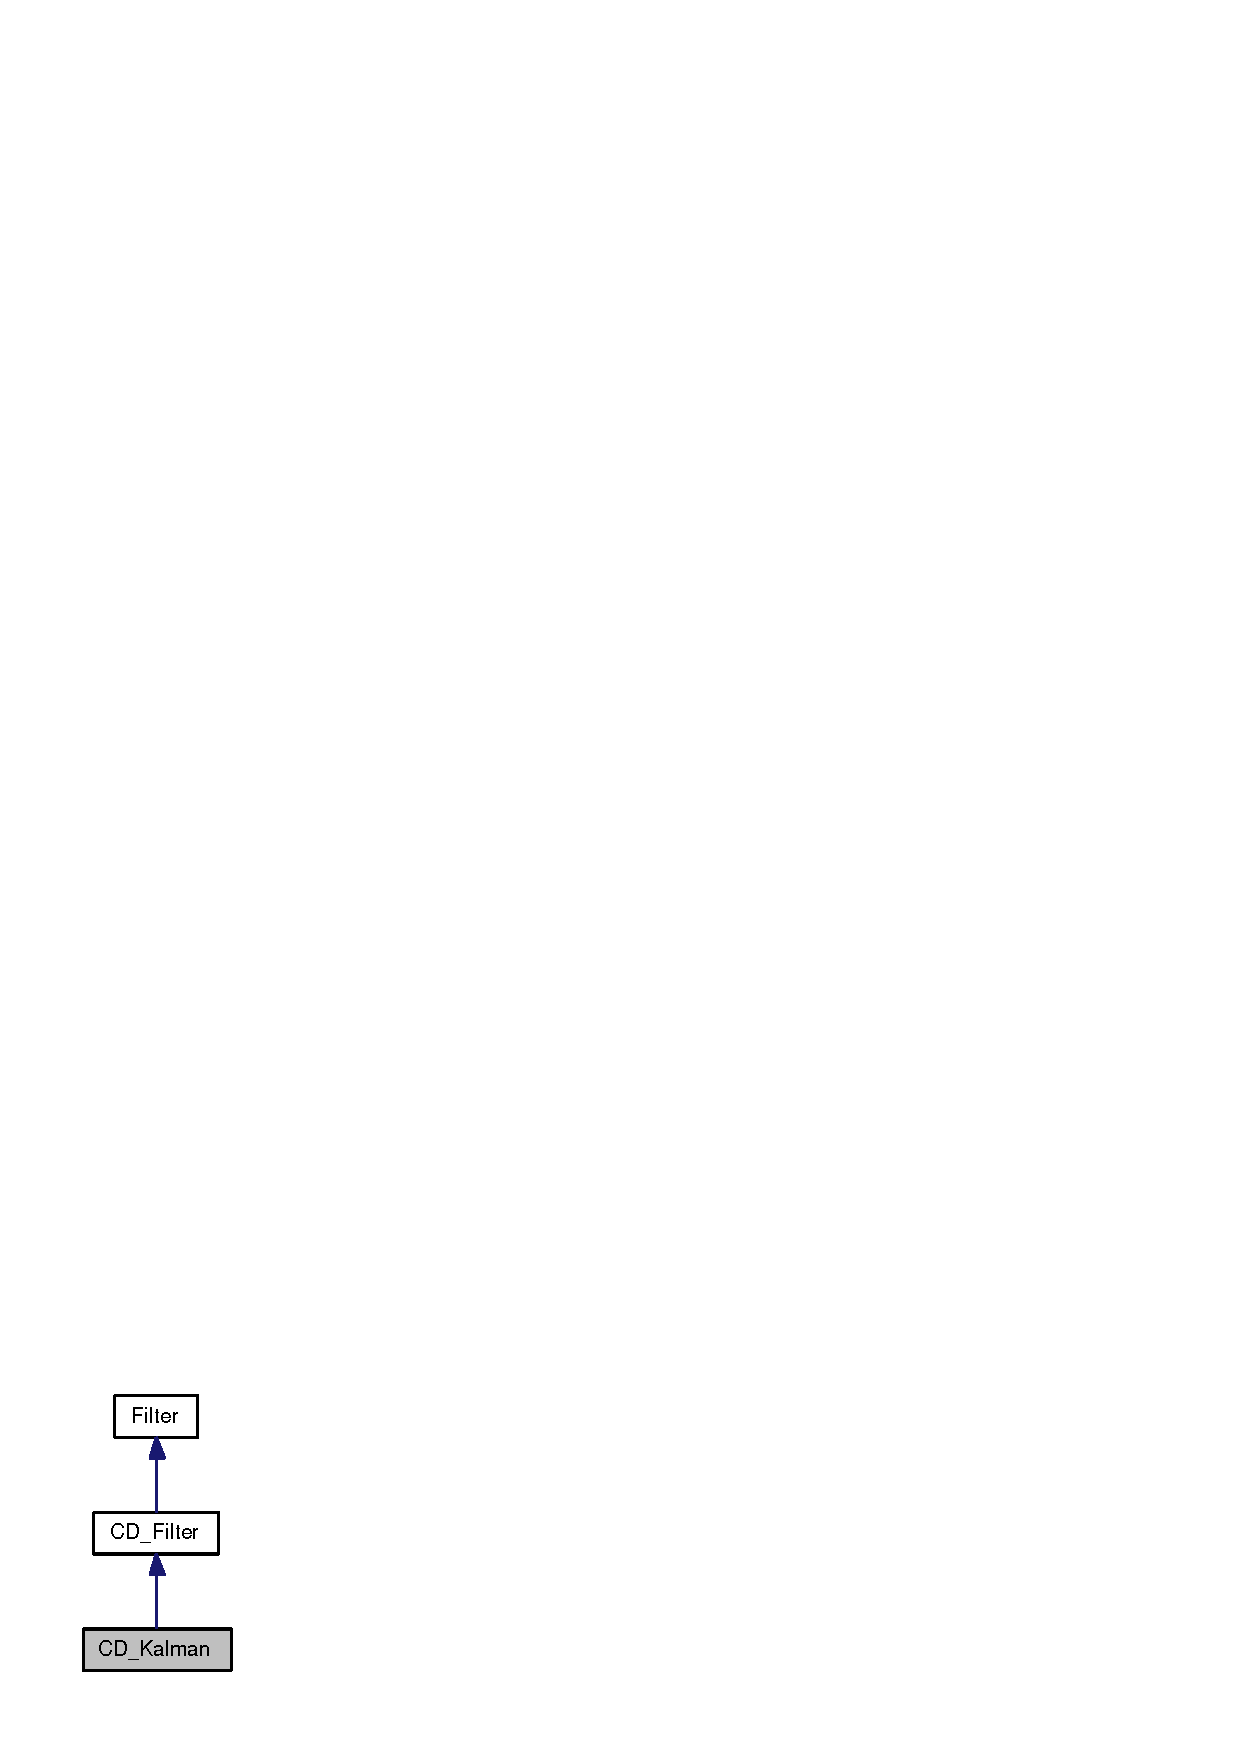
\includegraphics[width=57pt]{class_c_d___kalman__inherit__graph}
\end{center}
\end{figure}
\subsection*{Public Member Functions}
\begin{CompactItemize}
\item 
\hyperlink{class_c_d___kalman_d5d85ce755d9353740f4b9ffdf63455f}{CD\_\-Kalman} (void)
\item 
\hyperlink{class_c_d___kalman_0fd0cf5d85f0b5a820d2269bea6de350}{CD\_\-Kalman} (\hyperlink{class_linear___c_d___model}{Linear\_\-CD\_\-Model} $\ast$m)
\end{CompactItemize}
\subsection*{Protected Member Functions}
\begin{CompactItemize}
\item 
int \hyperlink{class_c_d___kalman_ecef658eac67b1005d9e86ec30708300}{\_\-update} (const dcovector \&Y)
\end{CompactItemize}


\subsection{Detailed Description}
The continuous-discrete kalman filter. 

Give an exact solution of $ \hat{X}_{k|k}$ and $ \hat{P}_{k|k} $ for continuous-discrete linear models (\hyperlink{class_linear___c_d___model}{Linear\_\-CD\_\-Model}). 

\subsection{Constructor \& Destructor Documentation}
\hypertarget{class_c_d___kalman_d5d85ce755d9353740f4b9ffdf63455f}{
\index{CD\_\-Kalman@{CD\_\-Kalman}!CD\_\-Kalman@{CD\_\-Kalman}}
\index{CD\_\-Kalman@{CD\_\-Kalman}!CD_Kalman@{CD\_\-Kalman}}
\subsubsection[{CD\_\-Kalman}]{\setlength{\rightskip}{0pt plus 5cm}CD\_\-Kalman::CD\_\-Kalman (void)}}
\label{class_c_d___kalman_d5d85ce755d9353740f4b9ffdf63455f}


\hypertarget{class_c_d___kalman_0fd0cf5d85f0b5a820d2269bea6de350}{
\index{CD\_\-Kalman@{CD\_\-Kalman}!CD\_\-Kalman@{CD\_\-Kalman}}
\index{CD\_\-Kalman@{CD\_\-Kalman}!CD_Kalman@{CD\_\-Kalman}}
\subsubsection[{CD\_\-Kalman}]{\setlength{\rightskip}{0pt plus 5cm}CD\_\-Kalman::CD\_\-Kalman ({\bf Linear\_\-CD\_\-Model} $\ast$ {\em m})}}
\label{class_c_d___kalman_0fd0cf5d85f0b5a820d2269bea6de350}


A constructor

\begin{Desc}
\item[Parameters:]
\begin{description}
\item[{\em m}]The continuous discrete model \end{description}
\end{Desc}


\subsection{Member Function Documentation}
\hypertarget{class_c_d___kalman_ecef658eac67b1005d9e86ec30708300}{
\index{CD\_\-Kalman@{CD\_\-Kalman}!\_\-update@{\_\-update}}
\index{\_\-update@{\_\-update}!CD_Kalman@{CD\_\-Kalman}}
\subsubsection[{\_\-update}]{\setlength{\rightskip}{0pt plus 5cm}int CD\_\-Kalman::\_\-update (const dcovector \& {\em Y})\hspace{0.3cm}{\tt  \mbox{[}protected, virtual\mbox{]}}}}
\label{class_c_d___kalman_ecef658eac67b1005d9e86ec30708300}


Specific update for each filter

\begin{Desc}
\item[Parameters:]
\begin{description}
\item[{\em Y}]The observed sample\end{description}
\end{Desc}
\begin{Desc}
\item[Returns:]0 if no problem \end{Desc}


Implements \hyperlink{class_filter_20ecd17fed3b8f11a76c960fe5e7144b}{Filter}.
\hypertarget{class_c_d___simulator}{
\section{CD\_\-Simulator Class Reference}
\label{class_c_d___simulator}\index{CD\_\-Simulator@{CD\_\-Simulator}}
}
{\tt \#include $<$simulator.h$>$}

Inheritance diagram for CD\_\-Simulator:\nopagebreak
\begin{figure}[H]
\begin{center}
\leavevmode
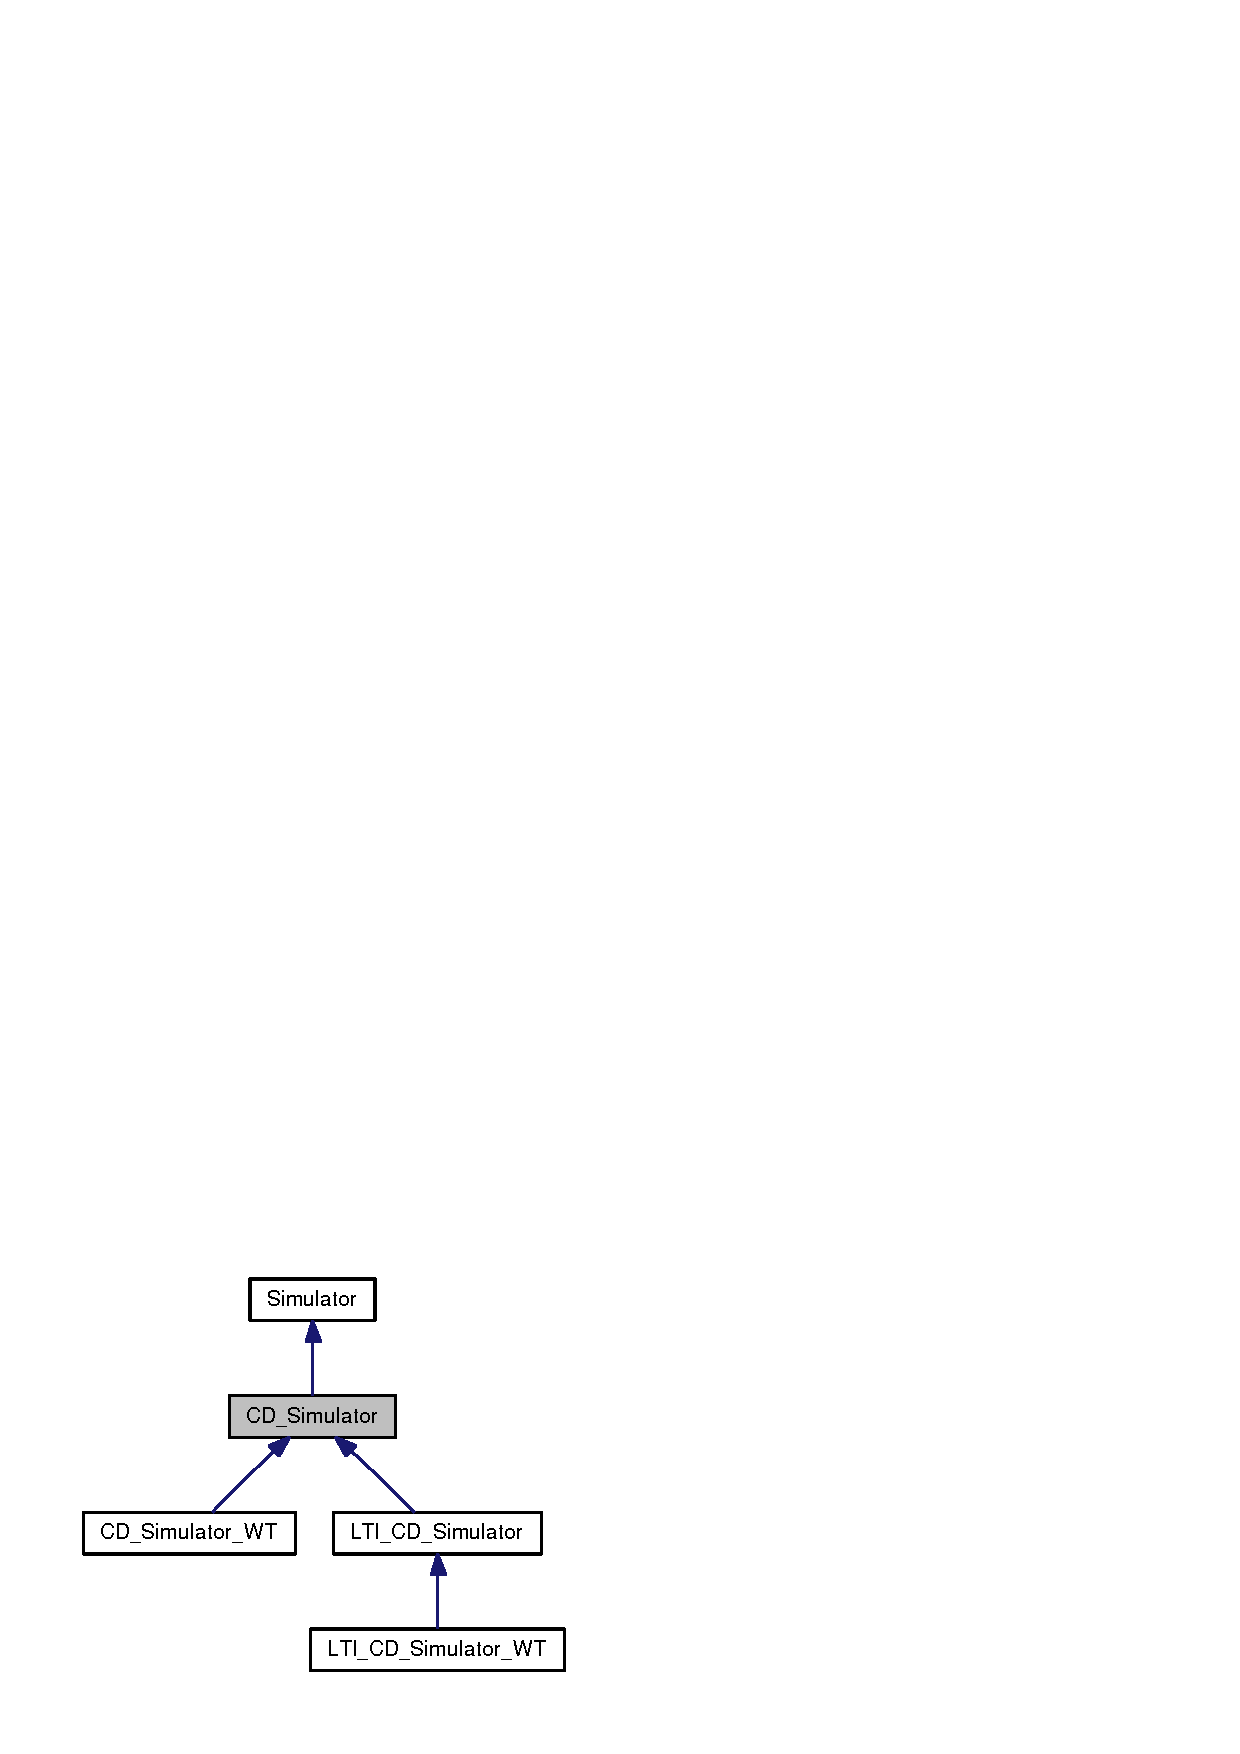
\includegraphics[width=137pt]{class_c_d___simulator__inherit__graph}
\end{center}
\end{figure}
\subsection*{Public Member Functions}
\begin{CompactItemize}
\item 
\hyperlink{class_c_d___simulator_c606f9720c399f258cbe89f24eecf83e}{CD\_\-Simulator} (void)
\item 
\hyperlink{class_c_d___simulator_e0a636e36d9c7821b34271d451b3b5a4}{CD\_\-Simulator} (\hyperlink{class_continuous___discrete___model}{Continuous\_\-Discrete\_\-Model} $\ast$cd\_\-m, const int \&\hyperlink{class_c_d___simulator_a19045bbd5c743d900780338ab355035}{scheme}=SRK4, const int \&apha=10)
\item 
virtual dcovector \hyperlink{class_c_d___simulator_cbdbea3e487026be0c032d2218d27b2b}{Draw\_\-Init} (void)
\begin{CompactList}\small\item\em Draw a sample from p(X0). \item\end{CompactList}\item 
dcovector \hyperlink{class_c_d___simulator_58019a5001ec77da3233b072f6328b30}{Draw\_\-Transition} (const dcovector \&Xkm1)
\begin{CompactList}\small\item\em Draw a sample from the transition densisty p(Xk$|$Xk-1). \item\end{CompactList}\item 
dcovector \hyperlink{class_c_d___simulator_3770eddf939898b6dccc39a556eaf8c9}{Draw\_\-Observation} (const dcovector \&Xk)
\begin{CompactList}\small\item\em Calculate the value of the density of probability of Y given X : p(Y$|$X). \item\end{CompactList}\item 
long double \hyperlink{class_c_d___simulator_905fb2ac4a72f5d7e44957fa8103cab8}{Observation\_\-Density} (const dcovector \&\hyperlink{class_simulator_403a127c909abf3e4c6d48a287315987}{Y}, const dcovector \&\hyperlink{class_simulator_a2db8ace19099d996be516022d230bc0}{X})
\begin{CompactList}\small\item\em calculate the value of the density of probability of Y given X : p(Y$|$X) \item\end{CompactList}\item 
int \hyperlink{class_c_d___simulator_7d9d7bb805654ee7ee1f2235364bc19e}{Save\_\-X} (const char $\ast$filename)
\begin{CompactList}\small\item\em Save the simulated state trajectory in filename. \item\end{CompactList}\item 
int \hyperlink{class_c_d___simulator_f9d3fb4fbc4b77afd81fb8b67e003cee}{Save\_\-Y} (const char $\ast$filename)
\begin{CompactList}\small\item\em Save the simulated observation trajectory in filename. \item\end{CompactList}\item 
int \hyperlink{class_c_d___simulator_fde7cba27399a95337431770b42b3772}{Simulate} (const double \&T)
\item 
void \hyperlink{class_c_d___simulator_6f78aafc96ae191c7b9815055ce4e956}{Set\_\-Alpha} (const int \&al)
\end{CompactItemize}
\subsection*{Public Attributes}
\begin{CompactItemize}
\item 
double \hyperlink{class_c_d___simulator_8c84fdf15866c0ea1cb79977f77639d2}{Dy}
\item 
double \hyperlink{class_c_d___simulator_adb3b1b1b8bd6deabea8a62fcec33138}{Dx}
\end{CompactItemize}
\subsection*{Protected Member Functions}
\begin{CompactItemize}
\item 
virtual dcovector \hyperlink{class_c_d___simulator_11c411df9b1e0d6f8576edefd723dd47}{draw\_\-state} (const dcovector \&\hyperlink{class_simulator_a2db8ace19099d996be516022d230bc0}{X})
\item 
void \hyperlink{class_c_d___simulator_efc4b4521a9d4cd6658c16feb9233e14}{\_\-update} (void)
\end{CompactItemize}
\subsection*{Protected Attributes}
\begin{CompactItemize}
\item 
int \hyperlink{class_c_d___simulator_a19045bbd5c743d900780338ab355035}{scheme}
\item 
int \hyperlink{class_c_d___simulator_f9d59b82e56e035230af9cf7d7767a9c}{\_\-a}
\end{CompactItemize}


\subsection{Constructor \& Destructor Documentation}
\hypertarget{class_c_d___simulator_c606f9720c399f258cbe89f24eecf83e}{
\index{CD\_\-Simulator@{CD\_\-Simulator}!CD\_\-Simulator@{CD\_\-Simulator}}
\index{CD\_\-Simulator@{CD\_\-Simulator}!CD_Simulator@{CD\_\-Simulator}}
\subsubsection[{CD\_\-Simulator}]{\setlength{\rightskip}{0pt plus 5cm}CD\_\-Simulator::CD\_\-Simulator (void)}}
\label{class_c_d___simulator_c606f9720c399f258cbe89f24eecf83e}


\hypertarget{class_c_d___simulator_e0a636e36d9c7821b34271d451b3b5a4}{
\index{CD\_\-Simulator@{CD\_\-Simulator}!CD\_\-Simulator@{CD\_\-Simulator}}
\index{CD\_\-Simulator@{CD\_\-Simulator}!CD_Simulator@{CD\_\-Simulator}}
\subsubsection[{CD\_\-Simulator}]{\setlength{\rightskip}{0pt plus 5cm}CD\_\-Simulator::CD\_\-Simulator ({\bf Continuous\_\-Discrete\_\-Model} $\ast$ {\em cd\_\-m}, \/  const int \& {\em scheme} = {\tt SRK4}, \/  const int \& {\em apha} = {\tt 10})}}
\label{class_c_d___simulator_e0a636e36d9c7821b34271d451b3b5a4}




\subsection{Member Function Documentation}
\hypertarget{class_c_d___simulator_efc4b4521a9d4cd6658c16feb9233e14}{
\index{CD\_\-Simulator@{CD\_\-Simulator}!\_\-update@{\_\-update}}
\index{\_\-update@{\_\-update}!CD_Simulator@{CD\_\-Simulator}}
\subsubsection[{\_\-update}]{\setlength{\rightskip}{0pt plus 5cm}void CD\_\-Simulator::\_\-update (void)\hspace{0.3cm}{\tt  \mbox{[}protected, virtual\mbox{]}}}}
\label{class_c_d___simulator_efc4b4521a9d4cd6658c16feb9233e14}




Reimplemented from \hyperlink{class_simulator_d4aa197c02a87ff2653b54c0b9207a33}{Simulator}.\hypertarget{class_c_d___simulator_cbdbea3e487026be0c032d2218d27b2b}{
\index{CD\_\-Simulator@{CD\_\-Simulator}!Draw\_\-Init@{Draw\_\-Init}}
\index{Draw\_\-Init@{Draw\_\-Init}!CD_Simulator@{CD\_\-Simulator}}
\subsubsection[{Draw\_\-Init}]{\setlength{\rightskip}{0pt plus 5cm}virtual dcovector CD\_\-Simulator::Draw\_\-Init (void)\hspace{0.3cm}{\tt  \mbox{[}virtual\mbox{]}}}}
\label{class_c_d___simulator_cbdbea3e487026be0c032d2218d27b2b}


Draw a sample from p(X0). 

\begin{Desc}
\item[Returns:]A sample from p(X0) \end{Desc}


Implements \hyperlink{class_simulator_29b9603eb2be9139972816329e8663dc}{Simulator}.

Reimplemented in \hyperlink{class_c_d___simulator___w_t_c05069bbef8e4ff83247f77476b2afe1}{CD\_\-Simulator\_\-WT}, and \hyperlink{class_l_t_i___c_d___simulator___w_t_a63eaac608a5f214468dc13d34f8f20f}{LTI\_\-CD\_\-Simulator\_\-WT}.\hypertarget{class_c_d___simulator_3770eddf939898b6dccc39a556eaf8c9}{
\index{CD\_\-Simulator@{CD\_\-Simulator}!Draw\_\-Observation@{Draw\_\-Observation}}
\index{Draw\_\-Observation@{Draw\_\-Observation}!CD_Simulator@{CD\_\-Simulator}}
\subsubsection[{Draw\_\-Observation}]{\setlength{\rightskip}{0pt plus 5cm}dcovector CD\_\-Simulator::Draw\_\-Observation (const dcovector \& {\em Xk})\hspace{0.3cm}{\tt  \mbox{[}virtual\mbox{]}}}}
\label{class_c_d___simulator_3770eddf939898b6dccc39a556eaf8c9}


Calculate the value of the density of probability of Y given X : p(Y$|$X). 

\begin{Desc}
\item[Parameters:]
\begin{description}
\item[{\em Xk}]The state at k\end{description}
\end{Desc}
\begin{Desc}
\item[Returns:]The simulated observation \end{Desc}


Implements \hyperlink{class_simulator_2fb966c2c2a4c93bb6788e15563c9006}{Simulator}.\hypertarget{class_c_d___simulator_11c411df9b1e0d6f8576edefd723dd47}{
\index{CD\_\-Simulator@{CD\_\-Simulator}!draw\_\-state@{draw\_\-state}}
\index{draw\_\-state@{draw\_\-state}!CD_Simulator@{CD\_\-Simulator}}
\subsubsection[{draw\_\-state}]{\setlength{\rightskip}{0pt plus 5cm}virtual dcovector CD\_\-Simulator::draw\_\-state (const dcovector \& {\em X})\hspace{0.3cm}{\tt  \mbox{[}protected, virtual\mbox{]}}}}
\label{class_c_d___simulator_11c411df9b1e0d6f8576edefd723dd47}




Reimplemented in \hyperlink{class_l_t_i___c_d___simulator_1497e233ff1a0d71c2b660fe270c9ff8}{LTI\_\-CD\_\-Simulator}.\hypertarget{class_c_d___simulator_58019a5001ec77da3233b072f6328b30}{
\index{CD\_\-Simulator@{CD\_\-Simulator}!Draw\_\-Transition@{Draw\_\-Transition}}
\index{Draw\_\-Transition@{Draw\_\-Transition}!CD_Simulator@{CD\_\-Simulator}}
\subsubsection[{Draw\_\-Transition}]{\setlength{\rightskip}{0pt plus 5cm}dcovector CD\_\-Simulator::Draw\_\-Transition (const dcovector \& {\em Xkm1})\hspace{0.3cm}{\tt  \mbox{[}virtual\mbox{]}}}}
\label{class_c_d___simulator_58019a5001ec77da3233b072f6328b30}


Draw a sample from the transition densisty p(Xk$|$Xk-1). 

\begin{Desc}
\item[Parameters:]
\begin{description}
\item[{\em Xkm1}]X(k-1) the preceding state\end{description}
\end{Desc}
\begin{Desc}
\item[Returns:]\end{Desc}


Implements \hyperlink{class_simulator_45790421a1c2f597739d3e972ad28292}{Simulator}.\hypertarget{class_c_d___simulator_905fb2ac4a72f5d7e44957fa8103cab8}{
\index{CD\_\-Simulator@{CD\_\-Simulator}!Observation\_\-Density@{Observation\_\-Density}}
\index{Observation\_\-Density@{Observation\_\-Density}!CD_Simulator@{CD\_\-Simulator}}
\subsubsection[{Observation\_\-Density}]{\setlength{\rightskip}{0pt plus 5cm}long double CD\_\-Simulator::Observation\_\-Density (const dcovector \& {\em Y}, \/  const dcovector \& {\em X})\hspace{0.3cm}{\tt  \mbox{[}virtual\mbox{]}}}}
\label{class_c_d___simulator_905fb2ac4a72f5d7e44957fa8103cab8}


calculate the value of the density of probability of Y given X : p(Y$|$X) 

\begin{Desc}
\item[Parameters:]
\begin{description}
\item[{\em Y}]The osbervation \item[{\em X}]The state\end{description}
\end{Desc}
\begin{Desc}
\item[Returns:]The value of the density \end{Desc}


Implements \hyperlink{class_simulator_75b0dfb5b0b88346ecb9f7da4fbd91f1}{Simulator}.\hypertarget{class_c_d___simulator_7d9d7bb805654ee7ee1f2235364bc19e}{
\index{CD\_\-Simulator@{CD\_\-Simulator}!Save\_\-X@{Save\_\-X}}
\index{Save\_\-X@{Save\_\-X}!CD_Simulator@{CD\_\-Simulator}}
\subsubsection[{Save\_\-X}]{\setlength{\rightskip}{0pt plus 5cm}int CD\_\-Simulator::Save\_\-X (const char $\ast$ {\em filename})\hspace{0.3cm}{\tt  \mbox{[}virtual\mbox{]}}}}
\label{class_c_d___simulator_7d9d7bb805654ee7ee1f2235364bc19e}


Save the simulated state trajectory in filename. 

\begin{Desc}
\item[Parameters:]
\begin{description}
\item[{\em filename}]The file\end{description}
\end{Desc}
\begin{Desc}
\item[Returns:]0 if it's ok \end{Desc}


Reimplemented from \hyperlink{class_simulator_47da05750f6f78051dcdecb5da666653}{Simulator}.\hypertarget{class_c_d___simulator_f9d3fb4fbc4b77afd81fb8b67e003cee}{
\index{CD\_\-Simulator@{CD\_\-Simulator}!Save\_\-Y@{Save\_\-Y}}
\index{Save\_\-Y@{Save\_\-Y}!CD_Simulator@{CD\_\-Simulator}}
\subsubsection[{Save\_\-Y}]{\setlength{\rightskip}{0pt plus 5cm}int CD\_\-Simulator::Save\_\-Y (const char $\ast$ {\em filename})\hspace{0.3cm}{\tt  \mbox{[}virtual\mbox{]}}}}
\label{class_c_d___simulator_f9d3fb4fbc4b77afd81fb8b67e003cee}


Save the simulated observation trajectory in filename. 

\begin{Desc}
\item[Parameters:]
\begin{description}
\item[{\em filename}]The file\end{description}
\end{Desc}
\begin{Desc}
\item[Returns:]0 if it's ok \end{Desc}


Reimplemented from \hyperlink{class_simulator_2cc53f33162bf08a6ae187ad4d34fe6e}{Simulator}.\hypertarget{class_c_d___simulator_6f78aafc96ae191c7b9815055ce4e956}{
\index{CD\_\-Simulator@{CD\_\-Simulator}!Set\_\-Alpha@{Set\_\-Alpha}}
\index{Set\_\-Alpha@{Set\_\-Alpha}!CD_Simulator@{CD\_\-Simulator}}
\subsubsection[{Set\_\-Alpha}]{\setlength{\rightskip}{0pt plus 5cm}void CD\_\-Simulator::Set\_\-Alpha (const int \& {\em al})}}
\label{class_c_d___simulator_6f78aafc96ae191c7b9815055ce4e956}


\hypertarget{class_c_d___simulator_fde7cba27399a95337431770b42b3772}{
\index{CD\_\-Simulator@{CD\_\-Simulator}!Simulate@{Simulate}}
\index{Simulate@{Simulate}!CD_Simulator@{CD\_\-Simulator}}
\subsubsection[{Simulate}]{\setlength{\rightskip}{0pt plus 5cm}int CD\_\-Simulator::Simulate (const double \& {\em T})}}
\label{class_c_d___simulator_fde7cba27399a95337431770b42b3772}




\subsection{Member Data Documentation}
\hypertarget{class_c_d___simulator_f9d59b82e56e035230af9cf7d7767a9c}{
\index{CD\_\-Simulator@{CD\_\-Simulator}!\_\-a@{\_\-a}}
\index{\_\-a@{\_\-a}!CD_Simulator@{CD\_\-Simulator}}
\subsubsection[{\_\-a}]{\setlength{\rightskip}{0pt plus 5cm}int {\bf CD\_\-Simulator::\_\-a}\hspace{0.3cm}{\tt  \mbox{[}protected\mbox{]}}}}
\label{class_c_d___simulator_f9d59b82e56e035230af9cf7d7767a9c}


\hypertarget{class_c_d___simulator_adb3b1b1b8bd6deabea8a62fcec33138}{
\index{CD\_\-Simulator@{CD\_\-Simulator}!Dx@{Dx}}
\index{Dx@{Dx}!CD_Simulator@{CD\_\-Simulator}}
\subsubsection[{Dx}]{\setlength{\rightskip}{0pt plus 5cm}double {\bf CD\_\-Simulator::Dx}}}
\label{class_c_d___simulator_adb3b1b1b8bd6deabea8a62fcec33138}


\hypertarget{class_c_d___simulator_8c84fdf15866c0ea1cb79977f77639d2}{
\index{CD\_\-Simulator@{CD\_\-Simulator}!Dy@{Dy}}
\index{Dy@{Dy}!CD_Simulator@{CD\_\-Simulator}}
\subsubsection[{Dy}]{\setlength{\rightskip}{0pt plus 5cm}double {\bf CD\_\-Simulator::Dy}}}
\label{class_c_d___simulator_8c84fdf15866c0ea1cb79977f77639d2}


\hypertarget{class_c_d___simulator_a19045bbd5c743d900780338ab355035}{
\index{CD\_\-Simulator@{CD\_\-Simulator}!scheme@{scheme}}
\index{scheme@{scheme}!CD_Simulator@{CD\_\-Simulator}}
\subsubsection[{scheme}]{\setlength{\rightskip}{0pt plus 5cm}int {\bf CD\_\-Simulator::scheme}\hspace{0.3cm}{\tt  \mbox{[}protected\mbox{]}}}}
\label{class_c_d___simulator_a19045bbd5c743d900780338ab355035}



\hypertarget{class_c_d___simulator___w_t}{
\section{CD\_\-Simulator\_\-WT Class Reference}
\label{class_c_d___simulator___w_t}\index{CD\_\-Simulator\_\-WT@{CD\_\-Simulator\_\-WT}}
}
{\tt \#include $<$simulator.h$>$}

Inheritance diagram for CD\_\-Simulator\_\-WT:\nopagebreak
\begin{figure}[H]
\begin{center}
\leavevmode
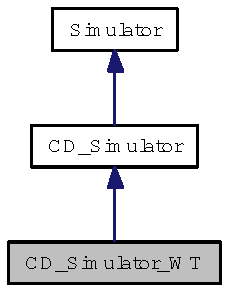
\includegraphics[width=73pt]{class_c_d___simulator___w_t__inherit__graph}
\end{center}
\end{figure}
\subsection*{Public Member Functions}
\begin{CompactItemize}
\item 
\hyperlink{class_c_d___simulator___w_t_83cf1b0723ca06211116b0478fa078b2}{CD\_\-Simulator\_\-WT} (void)
\item 
\hyperlink{class_c_d___simulator___w_t_173ec7213417756a63b91f9a7f3d18fd}{CD\_\-Simulator\_\-WT} (\hyperlink{class_continuous___discrete___model}{Continuous\_\-Discrete\_\-Model} $\ast$cd\_\-m, const int \&\hyperlink{class_c_d___simulator_a19045bbd5c743d900780338ab355035}{scheme}, const int \&apha, const double \&tb, const double \&t)
\item 
dcovector \hyperlink{class_c_d___simulator___w_t_c05069bbef8e4ff83247f77476b2afe1}{Draw\_\-Init} (void)
\begin{CompactList}\small\item\em Draw a sample from p(X0). \item\end{CompactList}\end{CompactItemize}
\subsection*{Private Attributes}
\begin{CompactItemize}
\item 
vector$<$ dcovector $>$ \hyperlink{class_c_d___simulator___w_t_eec47eb023c17590e9d1d89af874f1bc}{Xt}
\item 
double \hyperlink{class_c_d___simulator___w_t_5683b0d07bcb3f4f990ae261bb372487}{TB}
\item 
double \hyperlink{class_c_d___simulator___w_t_f6bede78aad1b7d023d5b139172a4103}{T}
\end{CompactItemize}


\subsection{Constructor \& Destructor Documentation}
\hypertarget{class_c_d___simulator___w_t_83cf1b0723ca06211116b0478fa078b2}{
\index{CD\_\-Simulator\_\-WT@{CD\_\-Simulator\_\-WT}!CD\_\-Simulator\_\-WT@{CD\_\-Simulator\_\-WT}}
\index{CD\_\-Simulator\_\-WT@{CD\_\-Simulator\_\-WT}!CD_Simulator_WT@{CD\_\-Simulator\_\-WT}}
\subsubsection[{CD\_\-Simulator\_\-WT}]{\setlength{\rightskip}{0pt plus 5cm}CD\_\-Simulator\_\-WT::CD\_\-Simulator\_\-WT (void)}}
\label{class_c_d___simulator___w_t_83cf1b0723ca06211116b0478fa078b2}


\hypertarget{class_c_d___simulator___w_t_173ec7213417756a63b91f9a7f3d18fd}{
\index{CD\_\-Simulator\_\-WT@{CD\_\-Simulator\_\-WT}!CD\_\-Simulator\_\-WT@{CD\_\-Simulator\_\-WT}}
\index{CD\_\-Simulator\_\-WT@{CD\_\-Simulator\_\-WT}!CD_Simulator_WT@{CD\_\-Simulator\_\-WT}}
\subsubsection[{CD\_\-Simulator\_\-WT}]{\setlength{\rightskip}{0pt plus 5cm}CD\_\-Simulator\_\-WT::CD\_\-Simulator\_\-WT ({\bf Continuous\_\-Discrete\_\-Model} $\ast$ {\em cd\_\-m}, \/  const int \& {\em scheme}, \/  const int \& {\em apha}, \/  const double \& {\em tb}, \/  const double \& {\em t})}}
\label{class_c_d___simulator___w_t_173ec7213417756a63b91f9a7f3d18fd}




\subsection{Member Function Documentation}
\hypertarget{class_c_d___simulator___w_t_c05069bbef8e4ff83247f77476b2afe1}{
\index{CD\_\-Simulator\_\-WT@{CD\_\-Simulator\_\-WT}!Draw\_\-Init@{Draw\_\-Init}}
\index{Draw\_\-Init@{Draw\_\-Init}!CD_Simulator_WT@{CD\_\-Simulator\_\-WT}}
\subsubsection[{Draw\_\-Init}]{\setlength{\rightskip}{0pt plus 5cm}dcovector CD\_\-Simulator\_\-WT::Draw\_\-Init (void)\hspace{0.3cm}{\tt  \mbox{[}virtual\mbox{]}}}}
\label{class_c_d___simulator___w_t_c05069bbef8e4ff83247f77476b2afe1}


Draw a sample from p(X0). 

\begin{Desc}
\item[Returns:]A sample from p(X0) \end{Desc}


Reimplemented from \hyperlink{class_c_d___simulator_cbdbea3e487026be0c032d2218d27b2b}{CD\_\-Simulator}.

\subsection{Member Data Documentation}
\hypertarget{class_c_d___simulator___w_t_f6bede78aad1b7d023d5b139172a4103}{
\index{CD\_\-Simulator\_\-WT@{CD\_\-Simulator\_\-WT}!T@{T}}
\index{T@{T}!CD_Simulator_WT@{CD\_\-Simulator\_\-WT}}
\subsubsection[{T}]{\setlength{\rightskip}{0pt plus 5cm}double {\bf CD\_\-Simulator\_\-WT::T}\hspace{0.3cm}{\tt  \mbox{[}private\mbox{]}}}}
\label{class_c_d___simulator___w_t_f6bede78aad1b7d023d5b139172a4103}


\hypertarget{class_c_d___simulator___w_t_5683b0d07bcb3f4f990ae261bb372487}{
\index{CD\_\-Simulator\_\-WT@{CD\_\-Simulator\_\-WT}!TB@{TB}}
\index{TB@{TB}!CD_Simulator_WT@{CD\_\-Simulator\_\-WT}}
\subsubsection[{TB}]{\setlength{\rightskip}{0pt plus 5cm}double {\bf CD\_\-Simulator\_\-WT::TB}\hspace{0.3cm}{\tt  \mbox{[}private\mbox{]}}}}
\label{class_c_d___simulator___w_t_5683b0d07bcb3f4f990ae261bb372487}


\hypertarget{class_c_d___simulator___w_t_eec47eb023c17590e9d1d89af874f1bc}{
\index{CD\_\-Simulator\_\-WT@{CD\_\-Simulator\_\-WT}!Xt@{Xt}}
\index{Xt@{Xt}!CD_Simulator_WT@{CD\_\-Simulator\_\-WT}}
\subsubsection[{Xt}]{\setlength{\rightskip}{0pt plus 5cm}vector$<$dcovector$>$ {\bf CD\_\-Simulator\_\-WT::Xt}\hspace{0.3cm}{\tt  \mbox{[}private\mbox{]}}}}
\label{class_c_d___simulator___w_t_eec47eb023c17590e9d1d89af874f1bc}



\hypertarget{class_continuous___discrete___model}{
\section{Continuous\_\-Discrete\_\-Model Class Reference}
\label{class_continuous___discrete___model}\index{Continuous\_\-Discrete\_\-Model@{Continuous\_\-Discrete\_\-Model}}
}
Continuous Discrete \hyperlink{class_model}{Model}: The continuous state : $ dX(t) = F(X)dt + G()*d\beta $ The discrete Observation $ Yk = H (X(tk)) + Vk $.  


{\tt \#include $<$gaussian\_\-model.h$>$}

Inheritance diagram for Continuous\_\-Discrete\_\-Model:\nopagebreak
\begin{figure}[H]
\begin{center}
\leavevmode
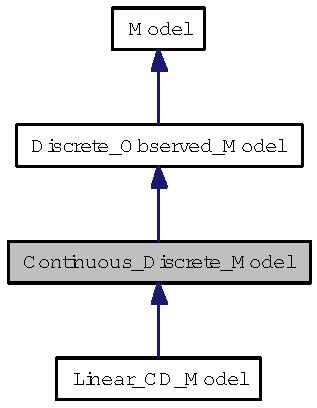
\includegraphics[width=94pt]{class_continuous___discrete___model__inherit__graph}
\end{center}
\end{figure}
\subsection*{Public Member Functions}
\begin{CompactItemize}
\item 
\hyperlink{class_continuous___discrete___model_fb738151cc4eb952d278d5531d10f97d}{Continuous\_\-Discrete\_\-Model} (void)
\item 
virtual \hyperlink{class_continuous___discrete___model_7c1ca102575a59207c3662181be1bdea}{$\sim$Continuous\_\-Discrete\_\-Model} (void)
\item 
virtual dcovector \hyperlink{class_continuous___discrete___model_fb901d0d92470ee3e2f5a06f74336b7d}{Drift\_\-Function} (const dcovector \&X)=0
\begin{CompactList}\small\item\em the drift function of dX(t) = F(X)dt + G(X)$\ast$dW \item\end{CompactList}\item 
virtual dgematrix \hyperlink{class_continuous___discrete___model_634d515a19cc782505935c8f23b00fff}{J\_\-Drift\_\-Function} (const dcovector \&X)
\begin{CompactList}\small\item\em the jacobian of the drift function evaluate at X \item\end{CompactList}\item 
virtual dgematrix \hyperlink{class_continuous___discrete___model_e305ba43f31be1275ede8d3d48d1d779}{Diffusion\_\-Function} (void)=0
\begin{CompactList}\small\item\em the diffusion function \item\end{CompactList}\item 
virtual void \hyperlink{class_continuous___discrete___model_fb787d768352c5a38048c35e51e7735d}{Init} (void)
\end{CompactItemize}
\subsection*{Public Attributes}
\begin{CompactItemize}
\item 
double \hyperlink{class_continuous___discrete___model_060335cf774016bc41c12a1c8421628c}{Ts}
\begin{CompactList}\small\item\em The sampling periode Ts=tk - tk-1. \item\end{CompactList}\end{CompactItemize}


\subsection{Detailed Description}
Continuous Discrete \hyperlink{class_model}{Model}: The continuous state : $ dX(t) = F(X)dt + G()*d\beta $ The discrete Observation $ Yk = H (X(tk)) + Vk $. 

\subsection{Constructor \& Destructor Documentation}
\hypertarget{class_continuous___discrete___model_fb738151cc4eb952d278d5531d10f97d}{
\index{Continuous\_\-Discrete\_\-Model@{Continuous\_\-Discrete\_\-Model}!Continuous\_\-Discrete\_\-Model@{Continuous\_\-Discrete\_\-Model}}
\index{Continuous\_\-Discrete\_\-Model@{Continuous\_\-Discrete\_\-Model}!Continuous_Discrete_Model@{Continuous\_\-Discrete\_\-Model}}
\subsubsection[{Continuous\_\-Discrete\_\-Model}]{\setlength{\rightskip}{0pt plus 5cm}Continuous\_\-Discrete\_\-Model::Continuous\_\-Discrete\_\-Model (void)}}
\label{class_continuous___discrete___model_fb738151cc4eb952d278d5531d10f97d}


The constructor \hypertarget{class_continuous___discrete___model_7c1ca102575a59207c3662181be1bdea}{
\index{Continuous\_\-Discrete\_\-Model@{Continuous\_\-Discrete\_\-Model}!$\sim$Continuous\_\-Discrete\_\-Model@{$\sim$Continuous\_\-Discrete\_\-Model}}
\index{$\sim$Continuous\_\-Discrete\_\-Model@{$\sim$Continuous\_\-Discrete\_\-Model}!Continuous_Discrete_Model@{Continuous\_\-Discrete\_\-Model}}
\subsubsection[{$\sim$Continuous\_\-Discrete\_\-Model}]{\setlength{\rightskip}{0pt plus 5cm}virtual Continuous\_\-Discrete\_\-Model::$\sim$Continuous\_\-Discrete\_\-Model (void)\hspace{0.3cm}{\tt  \mbox{[}virtual\mbox{]}}}}
\label{class_continuous___discrete___model_7c1ca102575a59207c3662181be1bdea}


The destructor 

\subsection{Member Function Documentation}
\hypertarget{class_continuous___discrete___model_e305ba43f31be1275ede8d3d48d1d779}{
\index{Continuous\_\-Discrete\_\-Model@{Continuous\_\-Discrete\_\-Model}!Diffusion\_\-Function@{Diffusion\_\-Function}}
\index{Diffusion\_\-Function@{Diffusion\_\-Function}!Continuous_Discrete_Model@{Continuous\_\-Discrete\_\-Model}}
\subsubsection[{Diffusion\_\-Function}]{\setlength{\rightskip}{0pt plus 5cm}virtual dgematrix Continuous\_\-Discrete\_\-Model::Diffusion\_\-Function (void)\hspace{0.3cm}{\tt  \mbox{[}pure virtual\mbox{]}}}}
\label{class_continuous___discrete___model_e305ba43f31be1275ede8d3d48d1d779}


the diffusion function 

\begin{Desc}
\item[Parameters:]
\begin{description}
\item[{\em X}]the state\end{description}
\end{Desc}
\begin{Desc}
\item[Returns:]G(X). \end{Desc}


Implemented in \hyperlink{class_linear___c_d___model_f6959eff1f30ff1772b05a45c5756054}{Linear\_\-CD\_\-Model}.\hypertarget{class_continuous___discrete___model_fb901d0d92470ee3e2f5a06f74336b7d}{
\index{Continuous\_\-Discrete\_\-Model@{Continuous\_\-Discrete\_\-Model}!Drift\_\-Function@{Drift\_\-Function}}
\index{Drift\_\-Function@{Drift\_\-Function}!Continuous_Discrete_Model@{Continuous\_\-Discrete\_\-Model}}
\subsubsection[{Drift\_\-Function}]{\setlength{\rightskip}{0pt plus 5cm}virtual dcovector Continuous\_\-Discrete\_\-Model::Drift\_\-Function (const dcovector \& {\em X})\hspace{0.3cm}{\tt  \mbox{[}pure virtual\mbox{]}}}}
\label{class_continuous___discrete___model_fb901d0d92470ee3e2f5a06f74336b7d}


the drift function of dX(t) = F(X)dt + G(X)$\ast$dW 

\begin{Desc}
\item[Parameters:]
\begin{description}
\item[{\em X}]the state.\end{description}
\end{Desc}
\begin{Desc}
\item[Returns:]f(X) \end{Desc}


Implemented in \hyperlink{class_linear___c_d___model_4a35ab32a6ff01885368d1b3690f4925}{Linear\_\-CD\_\-Model}.\hypertarget{class_continuous___discrete___model_fb787d768352c5a38048c35e51e7735d}{
\index{Continuous\_\-Discrete\_\-Model@{Continuous\_\-Discrete\_\-Model}!Init@{Init}}
\index{Init@{Init}!Continuous_Discrete_Model@{Continuous\_\-Discrete\_\-Model}}
\subsubsection[{Init}]{\setlength{\rightskip}{0pt plus 5cm}virtual void Continuous\_\-Discrete\_\-Model::Init (void)\hspace{0.3cm}{\tt  \mbox{[}inline, virtual\mbox{]}}}}
\label{class_continuous___discrete___model_fb787d768352c5a38048c35e51e7735d}


Initialized CD model 

Reimplemented in \hyperlink{class_linear___c_d___model_c115137cf3ae0d1670880d5a8b0a8bd4}{Linear\_\-CD\_\-Model}.\hypertarget{class_continuous___discrete___model_634d515a19cc782505935c8f23b00fff}{
\index{Continuous\_\-Discrete\_\-Model@{Continuous\_\-Discrete\_\-Model}!J\_\-Drift\_\-Function@{J\_\-Drift\_\-Function}}
\index{J\_\-Drift\_\-Function@{J\_\-Drift\_\-Function}!Continuous_Discrete_Model@{Continuous\_\-Discrete\_\-Model}}
\subsubsection[{J\_\-Drift\_\-Function}]{\setlength{\rightskip}{0pt plus 5cm}virtual dgematrix Continuous\_\-Discrete\_\-Model::J\_\-Drift\_\-Function (const dcovector \& {\em X})\hspace{0.3cm}{\tt  \mbox{[}virtual\mbox{]}}}}
\label{class_continuous___discrete___model_634d515a19cc782505935c8f23b00fff}


the jacobian of the drift function evaluate at X 

\begin{Desc}
\item[Parameters:]
\begin{description}
\item[{\em X}]\end{description}
\end{Desc}
\begin{Desc}
\item[Returns:]the jacobian matrix \end{Desc}


Reimplemented in \hyperlink{class_linear___c_d___model_6d063fdeaeba656c8449e1539f422e1a}{Linear\_\-CD\_\-Model}.

\subsection{Member Data Documentation}
\hypertarget{class_continuous___discrete___model_060335cf774016bc41c12a1c8421628c}{
\index{Continuous\_\-Discrete\_\-Model@{Continuous\_\-Discrete\_\-Model}!Ts@{Ts}}
\index{Ts@{Ts}!Continuous_Discrete_Model@{Continuous\_\-Discrete\_\-Model}}
\subsubsection[{Ts}]{\setlength{\rightskip}{0pt plus 5cm}double {\bf Continuous\_\-Discrete\_\-Model::Ts}}}
\label{class_continuous___discrete___model_060335cf774016bc41c12a1c8421628c}


The sampling periode Ts=tk - tk-1. 


\hypertarget{class_d_d___kalman}{
\section{DD\_\-Kalman Class Reference}
\label{class_d_d___kalman}\index{DD\_\-Kalman@{DD\_\-Kalman}}
}
The discrete-discrete kalman filter.  


{\tt \#include $<$filter.h$>$}

Inheritance diagram for DD\_\-Kalman:\nopagebreak
\begin{figure}[H]
\begin{center}
\leavevmode
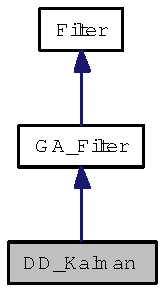
\includegraphics[width=57pt]{class_d_d___kalman__inherit__graph}
\end{center}
\end{figure}
\subsection*{Public Member Functions}
\begin{CompactItemize}
\item 
\hyperlink{class_d_d___kalman_6609717ac09c6a85dfbd1417b736a54c}{DD\_\-Kalman} (void)
\item 
\hyperlink{class_d_d___kalman_dfc3b894cf701465b05ed9b49a53f49e}{DD\_\-Kalman} (\hyperlink{class_gaussian___linear___model}{Gaussian\_\-Linear\_\-Model} $\ast$m)
\end{CompactItemize}
\subsection*{Protected Member Functions}
\begin{CompactItemize}
\item 
int \hyperlink{class_d_d___kalman_a04e9be77c495296673227860833c9fc}{\_\-update} (const dcovector \&Y)
\end{CompactItemize}


\subsection{Detailed Description}
The discrete-discrete kalman filter. 

Give an exact solution of $ \hat{X}_{k|k}$ and $ \hat{P}_{k|k} $ for discrete-discrete linear models (\hyperlink{class_gaussian___linear___model}{Gaussian\_\-Linear\_\-Model}). 

\subsection{Constructor \& Destructor Documentation}
\hypertarget{class_d_d___kalman_6609717ac09c6a85dfbd1417b736a54c}{
\index{DD\_\-Kalman@{DD\_\-Kalman}!DD\_\-Kalman@{DD\_\-Kalman}}
\index{DD\_\-Kalman@{DD\_\-Kalman}!DD_Kalman@{DD\_\-Kalman}}
\subsubsection[{DD\_\-Kalman}]{\setlength{\rightskip}{0pt plus 5cm}DD\_\-Kalman::DD\_\-Kalman (void)}}
\label{class_d_d___kalman_6609717ac09c6a85dfbd1417b736a54c}


\hypertarget{class_d_d___kalman_dfc3b894cf701465b05ed9b49a53f49e}{
\index{DD\_\-Kalman@{DD\_\-Kalman}!DD\_\-Kalman@{DD\_\-Kalman}}
\index{DD\_\-Kalman@{DD\_\-Kalman}!DD_Kalman@{DD\_\-Kalman}}
\subsubsection[{DD\_\-Kalman}]{\setlength{\rightskip}{0pt plus 5cm}DD\_\-Kalman::DD\_\-Kalman ({\bf Gaussian\_\-Linear\_\-Model} $\ast$ {\em m})}}
\label{class_d_d___kalman_dfc3b894cf701465b05ed9b49a53f49e}


A constructor

\begin{Desc}
\item[Parameters:]
\begin{description}
\item[{\em m}]The discrete-discrete model \end{description}
\end{Desc}


\subsection{Member Function Documentation}
\hypertarget{class_d_d___kalman_a04e9be77c495296673227860833c9fc}{
\index{DD\_\-Kalman@{DD\_\-Kalman}!\_\-update@{\_\-update}}
\index{\_\-update@{\_\-update}!DD_Kalman@{DD\_\-Kalman}}
\subsubsection[{\_\-update}]{\setlength{\rightskip}{0pt plus 5cm}int DD\_\-Kalman::\_\-update (const dcovector \& {\em Y})\hspace{0.3cm}{\tt  \mbox{[}protected, virtual\mbox{]}}}}
\label{class_d_d___kalman_a04e9be77c495296673227860833c9fc}


Specific update for each filter

\begin{Desc}
\item[Parameters:]
\begin{description}
\item[{\em Y}]The observed sample\end{description}
\end{Desc}
\begin{Desc}
\item[Returns:]0 if no problem \end{Desc}


Implements \hyperlink{class_filter_20ecd17fed3b8f11a76c960fe5e7144b}{Filter}.
\hypertarget{class_discrete___approximation___c_d___model}{
\section{Discrete\_\-Approximation\_\-CD\_\-Model Class Reference}
\label{class_discrete___approximation___c_d___model}\index{Discrete\_\-Approximation\_\-CD\_\-Model@{Discrete\_\-Approximation\_\-CD\_\-Model}}
}
the continuous state equation is discretly approximate by X(tk) = f'(X(tk-1),Wk)  


{\tt \#include $<$gaussian\_\-model.h$>$}

Inheritance diagram for Discrete\_\-Approximation\_\-CD\_\-Model:\nopagebreak
\begin{figure}[H]
\begin{center}
\leavevmode
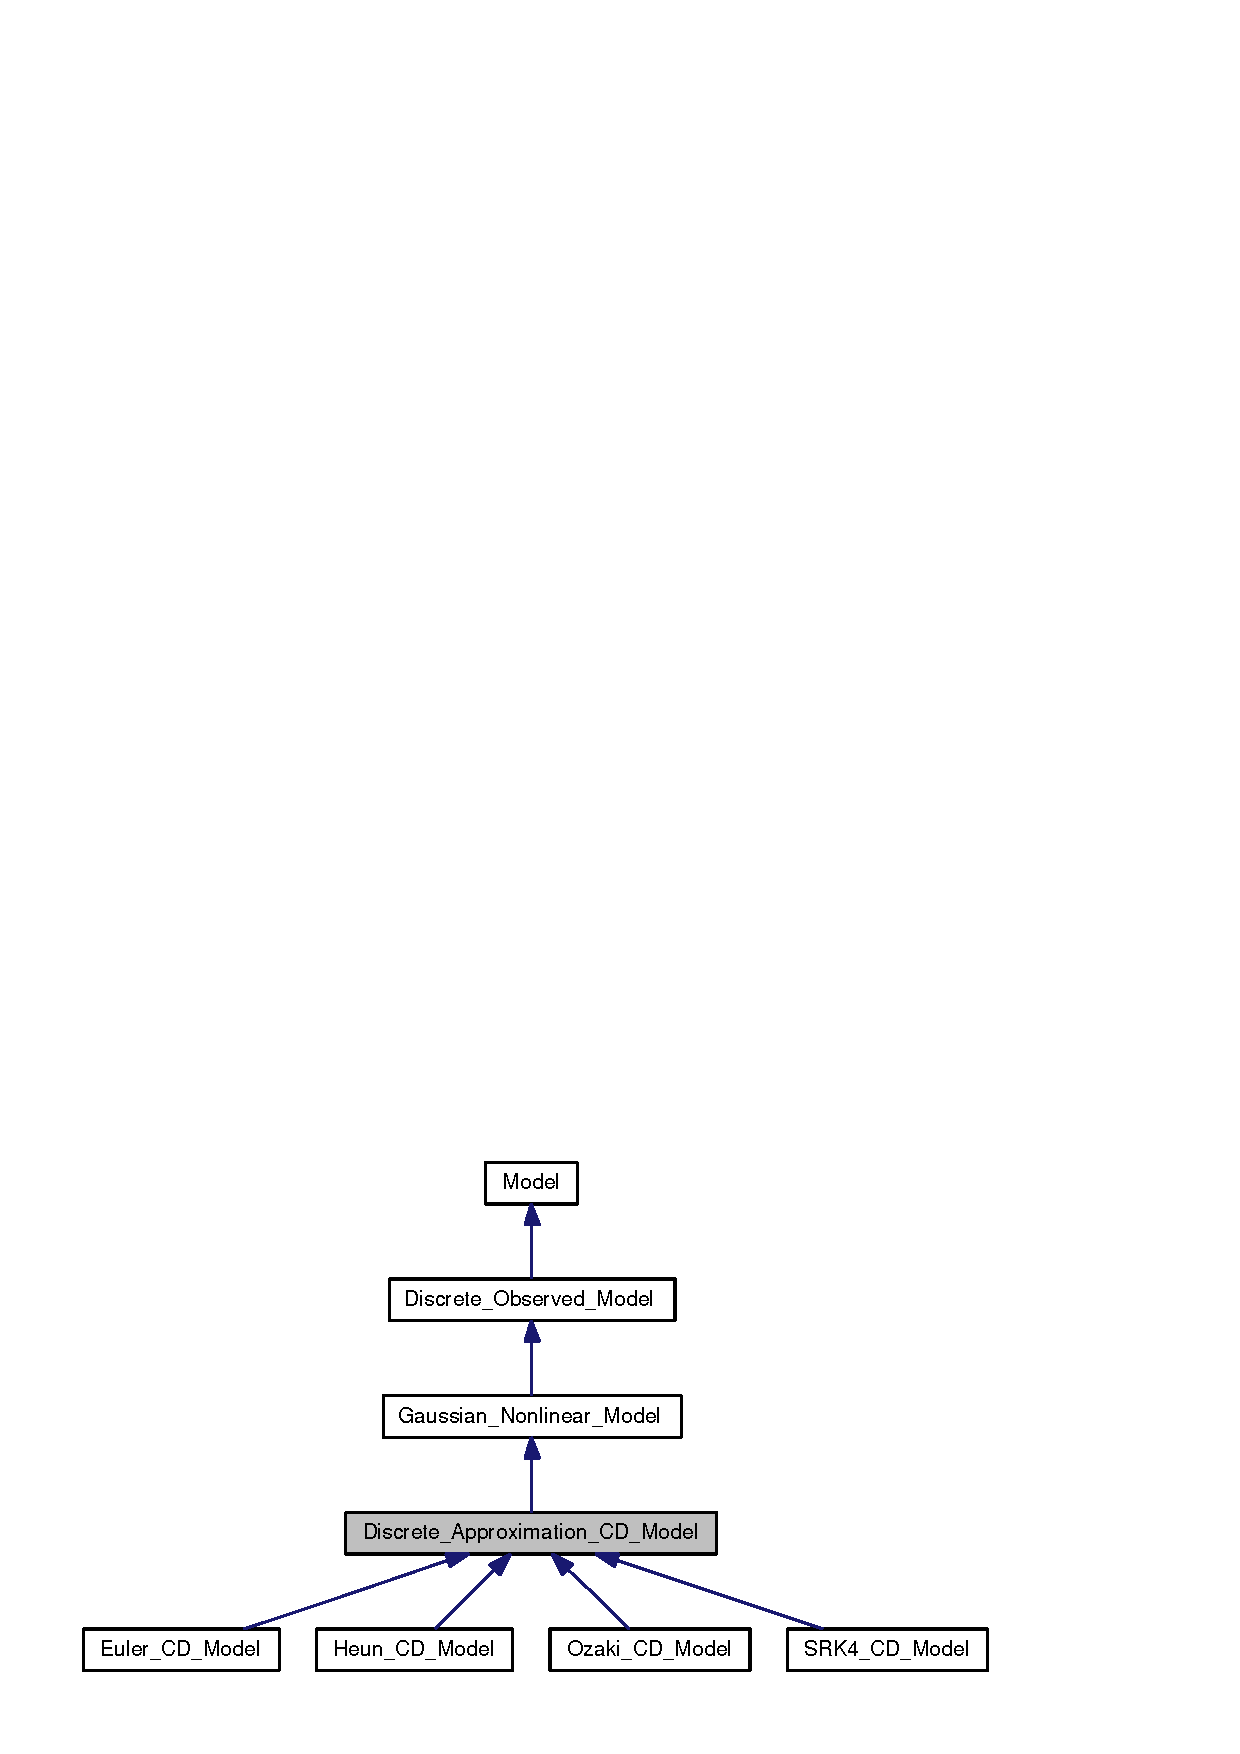
\includegraphics[width=400pt]{class_discrete___approximation___c_d___model__inherit__graph}
\end{center}
\end{figure}
\subsection*{Public Member Functions}
\begin{CompactItemize}
\item 
\hyperlink{class_discrete___approximation___c_d___model_89b9e3ef2887e000f1129eeef7038e6e}{Discrete\_\-Approximation\_\-CD\_\-Model} (void)
\item 
virtual \hyperlink{class_discrete___approximation___c_d___model_a9d8092144619d8a6a425662da7b29f8}{$\sim$Discrete\_\-Approximation\_\-CD\_\-Model} (void)
\item 
\hyperlink{class_discrete___approximation___c_d___model_36d4695074dc346ac6cba512a436012d}{Discrete\_\-Approximation\_\-CD\_\-Model} (\hyperlink{class_continuous___discrete___model}{Continuous\_\-Discrete\_\-Model} $\ast$m)
\item 
\hyperlink{class_discrete___approximation___c_d___model_564a37759c294b73299bbcb9f29897d1}{Discrete\_\-Approximation\_\-CD\_\-Model} (\hyperlink{class_continuous___discrete___model}{Continuous\_\-Discrete\_\-Model} $\ast$m, const int \&a)
\begin{CompactList}\small\item\em the constructor \item\end{CompactList}\item 
dcovector \hyperlink{class_discrete___approximation___c_d___model_83ef21b9993bfbef655874ca38777131}{State\_\-Function} (const dcovector \&X, const dcovector \&W)
\begin{CompactList}\small\item\em The state Xk=F(Xk-1,Wk). \item\end{CompactList}\item 
dgematrix \hyperlink{class_discrete___approximation___c_d___model_b0ba3cda373913f6a1df4a417200218a}{Jx\_\-State\_\-Function} (const dcovector \&X, const dcovector \&W)
\begin{CompactList}\small\item\em the X jacobian of the State function evaluate at X,W \item\end{CompactList}\item 
void \hyperlink{class_discrete___approximation___c_d___model_445e1215275e1f77f6260a186e9f842a}{Get\_\-Linear\_\-Parameters} (const dcovector \&X, const dcovector \&W, dgematrix \&F, dgematrix \&G, dcovector \&Xp)
\begin{CompactList}\small\item\em computed linearized parameter for EKF in X,W \item\end{CompactList}\item 
virtual void \hyperlink{class_discrete___approximation___c_d___model_0a486fada10e6f5569d186edc7b32110}{Get\_\-Linear\_\-Scheme} (const dcovector \&X, const dcovector \&W, dgematrix \&F, dgematrix \&J, dcovector \&Xp)=0
\begin{CompactList}\small\item\em Get the Linearized parameters Scheme in X,W. \item\end{CompactList}\item 
dgematrix \hyperlink{class_discrete___approximation___c_d___model_a5021c3ba6bd2cce5558a783843461ab}{Jw\_\-State\_\-Function} (const dcovector \&X, const dcovector \&W)
\begin{CompactList}\small\item\em the W jacobian of the State function evaluate at X,W \item\end{CompactList}\item 
dcovector \hyperlink{class_discrete___approximation___c_d___model_fe110c215bf843377888ad5ba823088e}{Observation\_\-Function} (const dcovector \&X)
\begin{CompactList}\small\item\em The observation Yk=H(Xk) + Vk. \item\end{CompactList}\item 
virtual dgematrix \hyperlink{class_discrete___approximation___c_d___model_be25ebdd3667dff8f8f43b72dc4e59ef}{J\_\-Observation\_\-Function} (const dcovector \&X)
\begin{CompactList}\small\item\em the jacobian of the observation function evaluate at X \item\end{CompactList}\item 
virtual dcovector \hyperlink{class_discrete___approximation___c_d___model_1ea9a1d618890fc51db6fa98eeb7af7f}{Scheme} (const dcovector \&X, const dcovector \&W)=0
\item 
virtual dgematrix \hyperlink{class_discrete___approximation___c_d___model_7a3dcae055d90be0b8a231eff961e2a2}{Jx\_\-Scheme} (const dcovector \&X, const dcovector \&W)=0
\item 
virtual dgematrix \hyperlink{class_discrete___approximation___c_d___model_c7496999409a3f05125ceb7fe85e85ab}{Jw\_\-Scheme} (const dcovector \&X, const dcovector \&W)=0
\item 
virtual void \hyperlink{class_discrete___approximation___c_d___model_0c4caaf9a2874a8e5219e72401caf908}{Init} (void)
\begin{CompactList}\small\item\em Init The model if needed. \item\end{CompactList}\item 
void \hyperlink{class_discrete___approximation___c_d___model_b6ebdd0ec42a24390d9446f10f7fa736}{Set\_\-Alpha} (const int \&a)
\item 
int \hyperlink{class_discrete___approximation___c_d___model_37b248fa0e24d9c70145ca546ee2a597}{Get\_\-Alpha} (void)
\end{CompactItemize}
\subsection*{Protected Attributes}
\begin{CompactItemize}
\item 
\hyperlink{class_continuous___discrete___model}{Continuous\_\-Discrete\_\-Model} $\ast$ \hyperlink{class_discrete___approximation___c_d___model_874071f4daae1dce9b15aaf5fc133846}{cd\_\-model}
\begin{CompactList}\small\item\em the continuous discrete model \item\end{CompactList}\item 
int \hyperlink{class_discrete___approximation___c_d___model_8200bfe0f27222f170057ca6d0ca123c}{alpha}
\begin{CompactList}\small\item\em the resolution of the discrete step Td = Ts $\ast$ a (Ts = sample duration of discrete observation) \item\end{CompactList}\end{CompactItemize}


\subsection{Detailed Description}
the continuous state equation is discretly approximate by X(tk) = f'(X(tk-1),Wk) 



\subsection{Constructor \& Destructor Documentation}
\hypertarget{class_discrete___approximation___c_d___model_89b9e3ef2887e000f1129eeef7038e6e}{
\index{Discrete\_\-Approximation\_\-CD\_\-Model@{Discrete\_\-Approximation\_\-CD\_\-Model}!Discrete\_\-Approximation\_\-CD\_\-Model@{Discrete\_\-Approximation\_\-CD\_\-Model}}
\index{Discrete\_\-Approximation\_\-CD\_\-Model@{Discrete\_\-Approximation\_\-CD\_\-Model}!Discrete_Approximation_CD_Model@{Discrete\_\-Approximation\_\-CD\_\-Model}}
\subsubsection[{Discrete\_\-Approximation\_\-CD\_\-Model}]{\setlength{\rightskip}{0pt plus 5cm}Discrete\_\-Approximation\_\-CD\_\-Model::Discrete\_\-Approximation\_\-CD\_\-Model (void)}}
\label{class_discrete___approximation___c_d___model_89b9e3ef2887e000f1129eeef7038e6e}


\hypertarget{class_discrete___approximation___c_d___model_a9d8092144619d8a6a425662da7b29f8}{
\index{Discrete\_\-Approximation\_\-CD\_\-Model@{Discrete\_\-Approximation\_\-CD\_\-Model}!$\sim$Discrete\_\-Approximation\_\-CD\_\-Model@{$\sim$Discrete\_\-Approximation\_\-CD\_\-Model}}
\index{$\sim$Discrete\_\-Approximation\_\-CD\_\-Model@{$\sim$Discrete\_\-Approximation\_\-CD\_\-Model}!Discrete_Approximation_CD_Model@{Discrete\_\-Approximation\_\-CD\_\-Model}}
\subsubsection[{$\sim$Discrete\_\-Approximation\_\-CD\_\-Model}]{\setlength{\rightskip}{0pt plus 5cm}virtual Discrete\_\-Approximation\_\-CD\_\-Model::$\sim$Discrete\_\-Approximation\_\-CD\_\-Model (void)\hspace{0.3cm}{\tt  \mbox{[}virtual\mbox{]}}}}
\label{class_discrete___approximation___c_d___model_a9d8092144619d8a6a425662da7b29f8}


\hypertarget{class_discrete___approximation___c_d___model_36d4695074dc346ac6cba512a436012d}{
\index{Discrete\_\-Approximation\_\-CD\_\-Model@{Discrete\_\-Approximation\_\-CD\_\-Model}!Discrete\_\-Approximation\_\-CD\_\-Model@{Discrete\_\-Approximation\_\-CD\_\-Model}}
\index{Discrete\_\-Approximation\_\-CD\_\-Model@{Discrete\_\-Approximation\_\-CD\_\-Model}!Discrete_Approximation_CD_Model@{Discrete\_\-Approximation\_\-CD\_\-Model}}
\subsubsection[{Discrete\_\-Approximation\_\-CD\_\-Model}]{\setlength{\rightskip}{0pt plus 5cm}Discrete\_\-Approximation\_\-CD\_\-Model::Discrete\_\-Approximation\_\-CD\_\-Model ({\bf Continuous\_\-Discrete\_\-Model} $\ast$ {\em m})}}
\label{class_discrete___approximation___c_d___model_36d4695074dc346ac6cba512a436012d}


\hypertarget{class_discrete___approximation___c_d___model_564a37759c294b73299bbcb9f29897d1}{
\index{Discrete\_\-Approximation\_\-CD\_\-Model@{Discrete\_\-Approximation\_\-CD\_\-Model}!Discrete\_\-Approximation\_\-CD\_\-Model@{Discrete\_\-Approximation\_\-CD\_\-Model}}
\index{Discrete\_\-Approximation\_\-CD\_\-Model@{Discrete\_\-Approximation\_\-CD\_\-Model}!Discrete_Approximation_CD_Model@{Discrete\_\-Approximation\_\-CD\_\-Model}}
\subsubsection[{Discrete\_\-Approximation\_\-CD\_\-Model}]{\setlength{\rightskip}{0pt plus 5cm}Discrete\_\-Approximation\_\-CD\_\-Model::Discrete\_\-Approximation\_\-CD\_\-Model ({\bf Continuous\_\-Discrete\_\-Model} $\ast$ {\em m}, \/  const int \& {\em a})}}
\label{class_discrete___approximation___c_d___model_564a37759c294b73299bbcb9f29897d1}


the constructor 

\begin{Desc}
\item[Parameters:]
\begin{description}
\item[{\em m}]the CD model \item[{\em a}]the resolution of the discrete step Td = Ts $\ast$ a (Ts = sample duration of discrete observation) \end{description}
\end{Desc}


\subsection{Member Function Documentation}
\hypertarget{class_discrete___approximation___c_d___model_37b248fa0e24d9c70145ca546ee2a597}{
\index{Discrete\_\-Approximation\_\-CD\_\-Model@{Discrete\_\-Approximation\_\-CD\_\-Model}!Get\_\-Alpha@{Get\_\-Alpha}}
\index{Get\_\-Alpha@{Get\_\-Alpha}!Discrete_Approximation_CD_Model@{Discrete\_\-Approximation\_\-CD\_\-Model}}
\subsubsection[{Get\_\-Alpha}]{\setlength{\rightskip}{0pt plus 5cm}int Discrete\_\-Approximation\_\-CD\_\-Model::Get\_\-Alpha (void)}}
\label{class_discrete___approximation___c_d___model_37b248fa0e24d9c70145ca546ee2a597}


\hypertarget{class_discrete___approximation___c_d___model_445e1215275e1f77f6260a186e9f842a}{
\index{Discrete\_\-Approximation\_\-CD\_\-Model@{Discrete\_\-Approximation\_\-CD\_\-Model}!Get\_\-Linear\_\-Parameters@{Get\_\-Linear\_\-Parameters}}
\index{Get\_\-Linear\_\-Parameters@{Get\_\-Linear\_\-Parameters}!Discrete_Approximation_CD_Model@{Discrete\_\-Approximation\_\-CD\_\-Model}}
\subsubsection[{Get\_\-Linear\_\-Parameters}]{\setlength{\rightskip}{0pt plus 5cm}void Discrete\_\-Approximation\_\-CD\_\-Model::Get\_\-Linear\_\-Parameters (const dcovector \& {\em X}, \/  const dcovector \& {\em W}, \/  dgematrix \& {\em F}, \/  dgematrix \& {\em G}, \/  dcovector \& {\em Xp})\hspace{0.3cm}{\tt  \mbox{[}virtual\mbox{]}}}}
\label{class_discrete___approximation___c_d___model_445e1215275e1f77f6260a186e9f842a}


computed linearized parameter for EKF in X,W 

\begin{Desc}
\item[Parameters:]
\begin{description}
\item[{\em X}]The state value \item[{\em W}]The noise value \item[{\em F}]The jacobian of f(X,W) in X \item[{\em G}]The jacobian in f(X,W) in W \item[{\em Xp}]The prediction Xp = f(X,W) \end{description}
\end{Desc}


Reimplemented from \hyperlink{class_gaussian___nonlinear___model_c850a678b4672e4358d3f29d7b998549}{Gaussian\_\-Nonlinear\_\-Model}.\hypertarget{class_discrete___approximation___c_d___model_0a486fada10e6f5569d186edc7b32110}{
\index{Discrete\_\-Approximation\_\-CD\_\-Model@{Discrete\_\-Approximation\_\-CD\_\-Model}!Get\_\-Linear\_\-Scheme@{Get\_\-Linear\_\-Scheme}}
\index{Get\_\-Linear\_\-Scheme@{Get\_\-Linear\_\-Scheme}!Discrete_Approximation_CD_Model@{Discrete\_\-Approximation\_\-CD\_\-Model}}
\subsubsection[{Get\_\-Linear\_\-Scheme}]{\setlength{\rightskip}{0pt plus 5cm}virtual void Discrete\_\-Approximation\_\-CD\_\-Model::Get\_\-Linear\_\-Scheme (const dcovector \& {\em X}, \/  const dcovector \& {\em W}, \/  dgematrix \& {\em F}, \/  dgematrix \& {\em J}, \/  dcovector \& {\em Xp})\hspace{0.3cm}{\tt  \mbox{[}pure virtual\mbox{]}}}}
\label{class_discrete___approximation___c_d___model_0a486fada10e6f5569d186edc7b32110}


Get the Linearized parameters Scheme in X,W. 

\begin{Desc}
\item[Parameters:]
\begin{description}
\item[{\em X}]The state value \item[{\em W}]The noise value \item[{\em F}]The jacobian of f(X,W) in X \item[{\em G}]The jacobian in f(X,W) in W \item[{\em Xp}]The prediction Xp = f(X,W) \end{description}
\end{Desc}


Implemented in \hyperlink{class_euler___c_d___model_e67b3130695db99e6057811914994aed}{Euler\_\-CD\_\-Model}, \hyperlink{class_s_r_k4___c_d___model_c348e8a59d0880ac366190004f4df36b}{SRK4\_\-CD\_\-Model}, \hyperlink{class_heun___c_d___model_38c51141d41b3c92509ab2c6040fd2cd}{Heun\_\-CD\_\-Model}, and \hyperlink{class_ozaki___c_d___model_c0878d9dda14cd1294e2ce7e5ab9c281}{Ozaki\_\-CD\_\-Model}.\hypertarget{class_discrete___approximation___c_d___model_0c4caaf9a2874a8e5219e72401caf908}{
\index{Discrete\_\-Approximation\_\-CD\_\-Model@{Discrete\_\-Approximation\_\-CD\_\-Model}!Init@{Init}}
\index{Init@{Init}!Discrete_Approximation_CD_Model@{Discrete\_\-Approximation\_\-CD\_\-Model}}
\subsubsection[{Init}]{\setlength{\rightskip}{0pt plus 5cm}virtual void Discrete\_\-Approximation\_\-CD\_\-Model::Init (void)\hspace{0.3cm}{\tt  \mbox{[}virtual\mbox{]}}}}
\label{class_discrete___approximation___c_d___model_0c4caaf9a2874a8e5219e72401caf908}


Init The model if needed. 



Reimplemented from \hyperlink{class_gaussian___nonlinear___model_146f819d0aeea0dc59b86e9af200e0bd}{Gaussian\_\-Nonlinear\_\-Model}.\hypertarget{class_discrete___approximation___c_d___model_be25ebdd3667dff8f8f43b72dc4e59ef}{
\index{Discrete\_\-Approximation\_\-CD\_\-Model@{Discrete\_\-Approximation\_\-CD\_\-Model}!J\_\-Observation\_\-Function@{J\_\-Observation\_\-Function}}
\index{J\_\-Observation\_\-Function@{J\_\-Observation\_\-Function}!Discrete_Approximation_CD_Model@{Discrete\_\-Approximation\_\-CD\_\-Model}}
\subsubsection[{J\_\-Observation\_\-Function}]{\setlength{\rightskip}{0pt plus 5cm}virtual dgematrix Discrete\_\-Approximation\_\-CD\_\-Model::J\_\-Observation\_\-Function (const dcovector \& {\em X})\hspace{0.3cm}{\tt  \mbox{[}virtual\mbox{]}}}}
\label{class_discrete___approximation___c_d___model_be25ebdd3667dff8f8f43b72dc4e59ef}


the jacobian of the observation function evaluate at X 

\begin{Desc}
\item[Parameters:]
\begin{description}
\item[{\em X}]\end{description}
\end{Desc}
\begin{Desc}
\item[Returns:]The jacobian matrix \end{Desc}


Reimplemented from \hyperlink{class_discrete___observed___model_83cd1f2f54544d8977dbce844031f85e}{Discrete\_\-Observed\_\-Model}.\hypertarget{class_discrete___approximation___c_d___model_c7496999409a3f05125ceb7fe85e85ab}{
\index{Discrete\_\-Approximation\_\-CD\_\-Model@{Discrete\_\-Approximation\_\-CD\_\-Model}!Jw\_\-Scheme@{Jw\_\-Scheme}}
\index{Jw\_\-Scheme@{Jw\_\-Scheme}!Discrete_Approximation_CD_Model@{Discrete\_\-Approximation\_\-CD\_\-Model}}
\subsubsection[{Jw\_\-Scheme}]{\setlength{\rightskip}{0pt plus 5cm}virtual dgematrix Discrete\_\-Approximation\_\-CD\_\-Model::Jw\_\-Scheme (const dcovector \& {\em X}, \/  const dcovector \& {\em W})\hspace{0.3cm}{\tt  \mbox{[}pure virtual\mbox{]}}}}
\label{class_discrete___approximation___c_d___model_c7496999409a3f05125ceb7fe85e85ab}




Implemented in \hyperlink{class_euler___c_d___model_d4b9cef601904d1e86c2f3a5f9e01b06}{Euler\_\-CD\_\-Model}, \hyperlink{class_s_r_k4___c_d___model_37045148c197b6143df008855179dfa3}{SRK4\_\-CD\_\-Model}, \hyperlink{class_heun___c_d___model_000fb9b8dbfb8171b8f330d7fc6d0dce}{Heun\_\-CD\_\-Model}, and \hyperlink{class_ozaki___c_d___model_66009069506580d175c869cea3df3cd6}{Ozaki\_\-CD\_\-Model}.\hypertarget{class_discrete___approximation___c_d___model_a5021c3ba6bd2cce5558a783843461ab}{
\index{Discrete\_\-Approximation\_\-CD\_\-Model@{Discrete\_\-Approximation\_\-CD\_\-Model}!Jw\_\-State\_\-Function@{Jw\_\-State\_\-Function}}
\index{Jw\_\-State\_\-Function@{Jw\_\-State\_\-Function}!Discrete_Approximation_CD_Model@{Discrete\_\-Approximation\_\-CD\_\-Model}}
\subsubsection[{Jw\_\-State\_\-Function}]{\setlength{\rightskip}{0pt plus 5cm}dgematrix Discrete\_\-Approximation\_\-CD\_\-Model::Jw\_\-State\_\-Function (const dcovector \& {\em X}, \/  const dcovector \& {\em W})\hspace{0.3cm}{\tt  \mbox{[}virtual\mbox{]}}}}
\label{class_discrete___approximation___c_d___model_a5021c3ba6bd2cce5558a783843461ab}


the W jacobian of the State function evaluate at X,W 

\begin{Desc}
\item[Parameters:]
\begin{description}
\item[{\em X}]evaluate at X \item[{\em W}]evalate at W\end{description}
\end{Desc}
\begin{Desc}
\item[Returns:]The jacobian matrix \end{Desc}


Reimplemented from \hyperlink{class_gaussian___nonlinear___model_1c6710cedf6317e07b7b2a48f41f5442}{Gaussian\_\-Nonlinear\_\-Model}.\hypertarget{class_discrete___approximation___c_d___model_7a3dcae055d90be0b8a231eff961e2a2}{
\index{Discrete\_\-Approximation\_\-CD\_\-Model@{Discrete\_\-Approximation\_\-CD\_\-Model}!Jx\_\-Scheme@{Jx\_\-Scheme}}
\index{Jx\_\-Scheme@{Jx\_\-Scheme}!Discrete_Approximation_CD_Model@{Discrete\_\-Approximation\_\-CD\_\-Model}}
\subsubsection[{Jx\_\-Scheme}]{\setlength{\rightskip}{0pt plus 5cm}virtual dgematrix Discrete\_\-Approximation\_\-CD\_\-Model::Jx\_\-Scheme (const dcovector \& {\em X}, \/  const dcovector \& {\em W})\hspace{0.3cm}{\tt  \mbox{[}pure virtual\mbox{]}}}}
\label{class_discrete___approximation___c_d___model_7a3dcae055d90be0b8a231eff961e2a2}




Implemented in \hyperlink{class_euler___c_d___model_31ea181a55cb1b348bd483f5fe077c50}{Euler\_\-CD\_\-Model}, \hyperlink{class_s_r_k4___c_d___model_2e0543a20a7ba52958606bda265413bd}{SRK4\_\-CD\_\-Model}, \hyperlink{class_heun___c_d___model_322cd83c0b81c2ed81483f42123f08e6}{Heun\_\-CD\_\-Model}, and \hyperlink{class_ozaki___c_d___model_6c4415b26674d1fc7b5e4f7499f35dd9}{Ozaki\_\-CD\_\-Model}.\hypertarget{class_discrete___approximation___c_d___model_b0ba3cda373913f6a1df4a417200218a}{
\index{Discrete\_\-Approximation\_\-CD\_\-Model@{Discrete\_\-Approximation\_\-CD\_\-Model}!Jx\_\-State\_\-Function@{Jx\_\-State\_\-Function}}
\index{Jx\_\-State\_\-Function@{Jx\_\-State\_\-Function}!Discrete_Approximation_CD_Model@{Discrete\_\-Approximation\_\-CD\_\-Model}}
\subsubsection[{Jx\_\-State\_\-Function}]{\setlength{\rightskip}{0pt plus 5cm}dgematrix Discrete\_\-Approximation\_\-CD\_\-Model::Jx\_\-State\_\-Function (const dcovector \& {\em X}, \/  const dcovector \& {\em W})\hspace{0.3cm}{\tt  \mbox{[}virtual\mbox{]}}}}
\label{class_discrete___approximation___c_d___model_b0ba3cda373913f6a1df4a417200218a}


the X jacobian of the State function evaluate at X,W 

\begin{Desc}
\item[Parameters:]
\begin{description}
\item[{\em X}]evaluate at X \item[{\em W}]evalate at W\end{description}
\end{Desc}
\begin{Desc}
\item[Returns:]The jacobian matrix \end{Desc}


Reimplemented from \hyperlink{class_gaussian___nonlinear___model_ad4a587fcaab06d2d9e44d61cee814cf}{Gaussian\_\-Nonlinear\_\-Model}.\hypertarget{class_discrete___approximation___c_d___model_fe110c215bf843377888ad5ba823088e}{
\index{Discrete\_\-Approximation\_\-CD\_\-Model@{Discrete\_\-Approximation\_\-CD\_\-Model}!Observation\_\-Function@{Observation\_\-Function}}
\index{Observation\_\-Function@{Observation\_\-Function}!Discrete_Approximation_CD_Model@{Discrete\_\-Approximation\_\-CD\_\-Model}}
\subsubsection[{Observation\_\-Function}]{\setlength{\rightskip}{0pt plus 5cm}dcovector Discrete\_\-Approximation\_\-CD\_\-Model::Observation\_\-Function (const dcovector \& {\em X})\hspace{0.3cm}{\tt  \mbox{[}virtual\mbox{]}}}}
\label{class_discrete___approximation___c_d___model_fe110c215bf843377888ad5ba823088e}


The observation Yk=H(Xk) + Vk. 

\begin{Desc}
\item[Parameters:]
\begin{description}
\item[{\em X}]The state at k\end{description}
\end{Desc}
\begin{Desc}
\item[Returns:]The observation at k \end{Desc}


Implements \hyperlink{class_discrete___observed___model_8d56d86ea6b204672c8ebd720f1e11a6}{Discrete\_\-Observed\_\-Model}.\hypertarget{class_discrete___approximation___c_d___model_1ea9a1d618890fc51db6fa98eeb7af7f}{
\index{Discrete\_\-Approximation\_\-CD\_\-Model@{Discrete\_\-Approximation\_\-CD\_\-Model}!Scheme@{Scheme}}
\index{Scheme@{Scheme}!Discrete_Approximation_CD_Model@{Discrete\_\-Approximation\_\-CD\_\-Model}}
\subsubsection[{Scheme}]{\setlength{\rightskip}{0pt plus 5cm}virtual dcovector Discrete\_\-Approximation\_\-CD\_\-Model::Scheme (const dcovector \& {\em X}, \/  const dcovector \& {\em W})\hspace{0.3cm}{\tt  \mbox{[}pure virtual\mbox{]}}}}
\label{class_discrete___approximation___c_d___model_1ea9a1d618890fc51db6fa98eeb7af7f}




Implemented in \hyperlink{class_euler___c_d___model_c113d0fdd6ba262f11ddfc0446827469}{Euler\_\-CD\_\-Model}, \hyperlink{class_s_r_k4___c_d___model_553c1dc82fe1e497ff73a919e6bd98e6}{SRK4\_\-CD\_\-Model}, \hyperlink{class_heun___c_d___model_98a85a23296e6c9f422f12063ece307b}{Heun\_\-CD\_\-Model}, and \hyperlink{class_ozaki___c_d___model_394a9716158c403c06c4416f01e661a9}{Ozaki\_\-CD\_\-Model}.\hypertarget{class_discrete___approximation___c_d___model_b6ebdd0ec42a24390d9446f10f7fa736}{
\index{Discrete\_\-Approximation\_\-CD\_\-Model@{Discrete\_\-Approximation\_\-CD\_\-Model}!Set\_\-Alpha@{Set\_\-Alpha}}
\index{Set\_\-Alpha@{Set\_\-Alpha}!Discrete_Approximation_CD_Model@{Discrete\_\-Approximation\_\-CD\_\-Model}}
\subsubsection[{Set\_\-Alpha}]{\setlength{\rightskip}{0pt plus 5cm}void Discrete\_\-Approximation\_\-CD\_\-Model::Set\_\-Alpha (const int \& {\em a})}}
\label{class_discrete___approximation___c_d___model_b6ebdd0ec42a24390d9446f10f7fa736}


\hypertarget{class_discrete___approximation___c_d___model_83ef21b9993bfbef655874ca38777131}{
\index{Discrete\_\-Approximation\_\-CD\_\-Model@{Discrete\_\-Approximation\_\-CD\_\-Model}!State\_\-Function@{State\_\-Function}}
\index{State\_\-Function@{State\_\-Function}!Discrete_Approximation_CD_Model@{Discrete\_\-Approximation\_\-CD\_\-Model}}
\subsubsection[{State\_\-Function}]{\setlength{\rightskip}{0pt plus 5cm}dcovector Discrete\_\-Approximation\_\-CD\_\-Model::State\_\-Function (const dcovector \& {\em X}, \/  const dcovector \& {\em W})\hspace{0.3cm}{\tt  \mbox{[}virtual\mbox{]}}}}
\label{class_discrete___approximation___c_d___model_83ef21b9993bfbef655874ca38777131}


The state Xk=F(Xk-1,Wk). 

\begin{Desc}
\item[Parameters:]
\begin{description}
\item[{\em X}]The state at k-1 \item[{\em W}]The Noise\end{description}
\end{Desc}
\begin{Desc}
\item[Returns:]The state at k \end{Desc}


Implements \hyperlink{class_gaussian___nonlinear___model_df0e6cf50a8d5fdb6decd05046867cd8}{Gaussian\_\-Nonlinear\_\-Model}.

\subsection{Member Data Documentation}
\hypertarget{class_discrete___approximation___c_d___model_8200bfe0f27222f170057ca6d0ca123c}{
\index{Discrete\_\-Approximation\_\-CD\_\-Model@{Discrete\_\-Approximation\_\-CD\_\-Model}!alpha@{alpha}}
\index{alpha@{alpha}!Discrete_Approximation_CD_Model@{Discrete\_\-Approximation\_\-CD\_\-Model}}
\subsubsection[{alpha}]{\setlength{\rightskip}{0pt plus 5cm}int {\bf Discrete\_\-Approximation\_\-CD\_\-Model::alpha}\hspace{0.3cm}{\tt  \mbox{[}protected\mbox{]}}}}
\label{class_discrete___approximation___c_d___model_8200bfe0f27222f170057ca6d0ca123c}


the resolution of the discrete step Td = Ts $\ast$ a (Ts = sample duration of discrete observation) 

\hypertarget{class_discrete___approximation___c_d___model_874071f4daae1dce9b15aaf5fc133846}{
\index{Discrete\_\-Approximation\_\-CD\_\-Model@{Discrete\_\-Approximation\_\-CD\_\-Model}!cd\_\-model@{cd\_\-model}}
\index{cd\_\-model@{cd\_\-model}!Discrete_Approximation_CD_Model@{Discrete\_\-Approximation\_\-CD\_\-Model}}
\subsubsection[{cd\_\-model}]{\setlength{\rightskip}{0pt plus 5cm}{\bf Continuous\_\-Discrete\_\-Model}$\ast$ {\bf Discrete\_\-Approximation\_\-CD\_\-Model::cd\_\-model}\hspace{0.3cm}{\tt  \mbox{[}protected\mbox{]}}}}
\label{class_discrete___approximation___c_d___model_874071f4daae1dce9b15aaf5fc133846}


the continuous discrete model 


\hypertarget{class_discrete___observed___model}{
\section{Discrete\_\-Observed\_\-Model Class Reference}
\label{class_discrete___observed___model}\index{Discrete\_\-Observed\_\-Model@{Discrete\_\-Observed\_\-Model}}
}
Class of discretely observed model.  


{\tt \#include $<$gaussian\_\-model.h$>$}

Inheritance diagram for Discrete\_\-Observed\_\-Model:\nopagebreak
\begin{figure}[H]
\begin{center}
\leavevmode
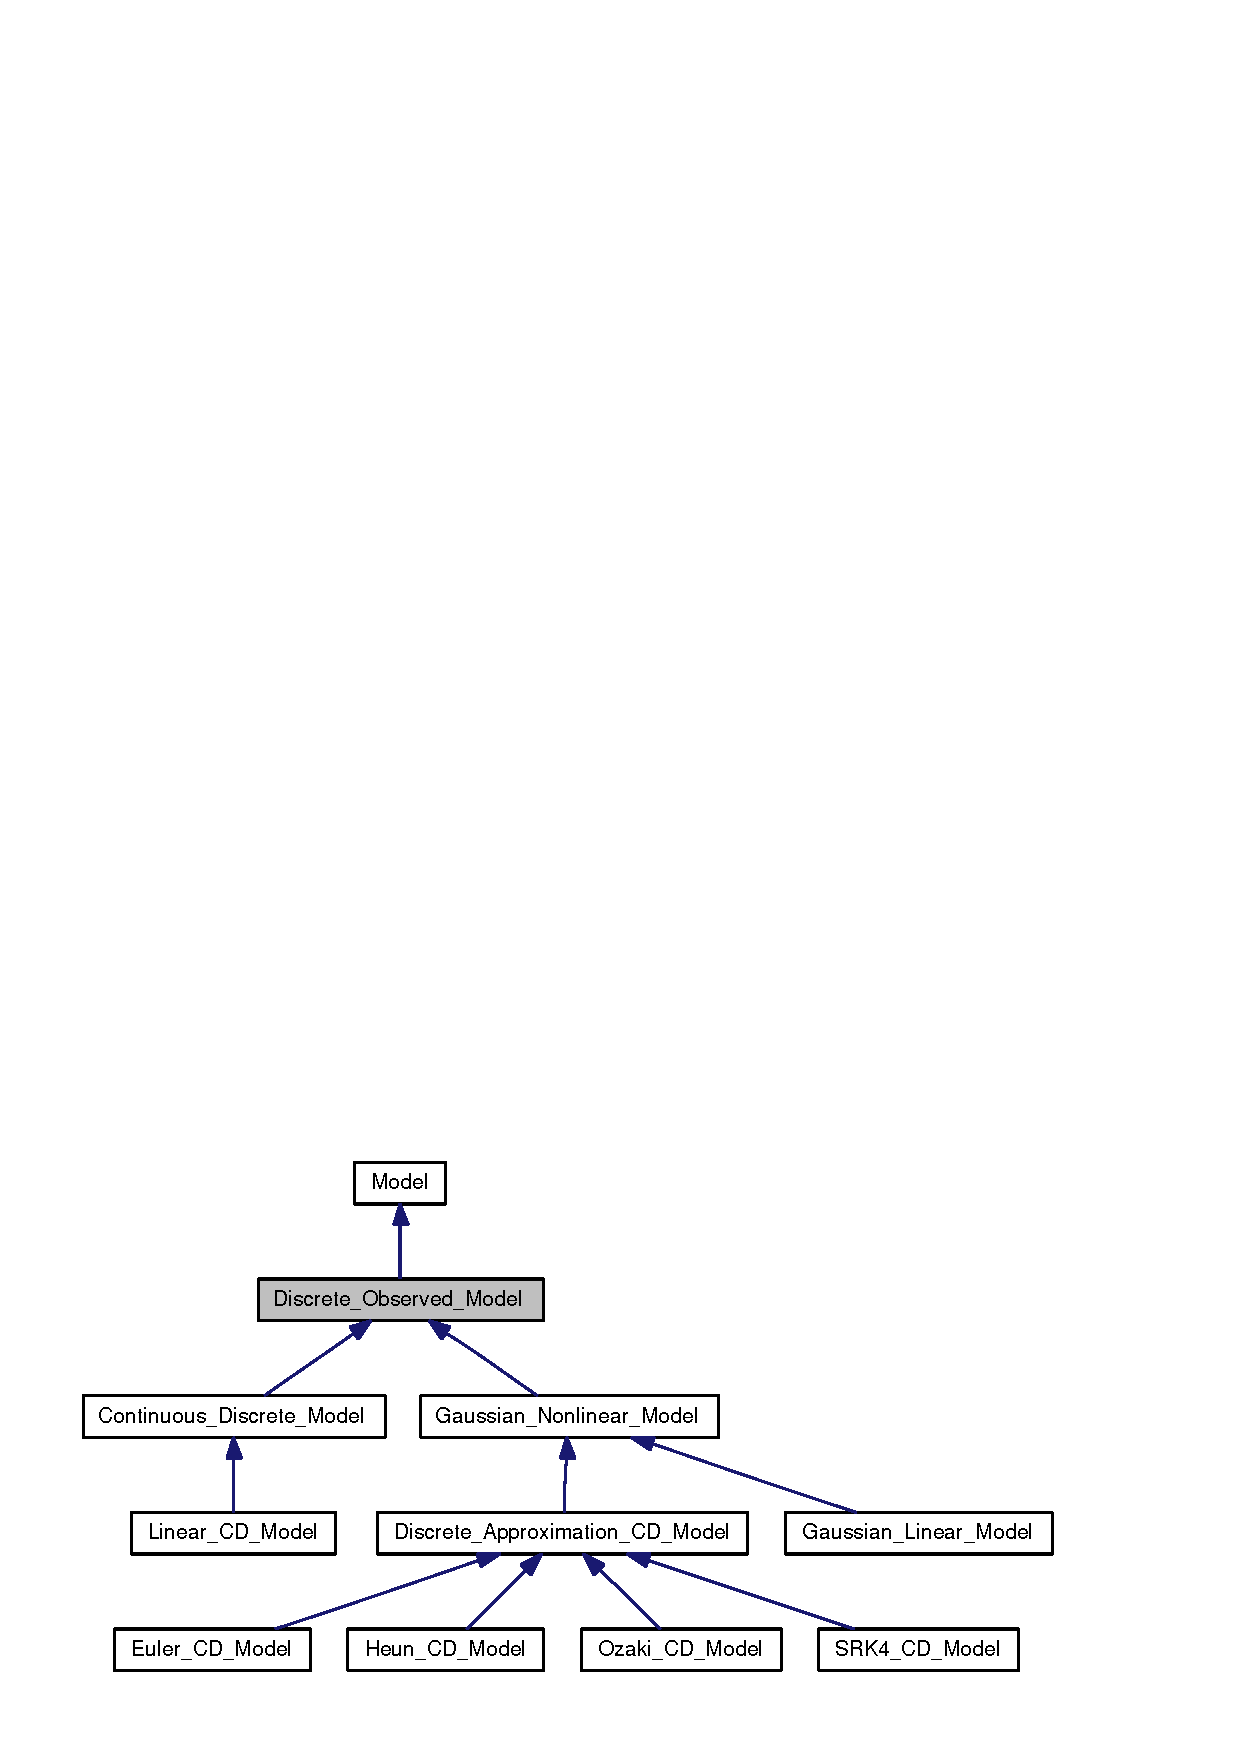
\includegraphics[width=400pt]{class_discrete___observed___model__inherit__graph}
\end{center}
\end{figure}
\subsection*{Public Member Functions}
\begin{CompactItemize}
\item 
\hyperlink{class_discrete___observed___model_919fa5f92fc705c4b2b3b7c94c0517ef}{Discrete\_\-Observed\_\-Model} (void)
\begin{CompactList}\small\item\em The Constructor. \item\end{CompactList}\item 
virtual \hyperlink{class_discrete___observed___model_8439d77622a8479eded60eeb51fcb5c6}{$\sim$Discrete\_\-Observed\_\-Model} (void)
\begin{CompactList}\small\item\em The Destructor. \item\end{CompactList}\item 
virtual dcovector \hyperlink{class_discrete___observed___model_8d56d86ea6b204672c8ebd720f1e11a6}{Observation\_\-Function} (const dcovector \&X)=0
\begin{CompactList}\small\item\em The observation Yk=H(Xk) + Vk. \item\end{CompactList}\item 
virtual dgematrix \hyperlink{class_discrete___observed___model_83cd1f2f54544d8977dbce844031f85e}{J\_\-Observation\_\-Function} (const dcovector \&X)
\begin{CompactList}\small\item\em the jacobian of the observation function evaluate at X \item\end{CompactList}\item 
virtual void \hyperlink{class_discrete___observed___model_e10c283d482bdb9257ad87a9cf5e6898}{Get\_\-Init\_\-Parameters} (dcovector \&mean, dsymatrix \&Cov)
\begin{CompactList}\small\item\em Return the first an second moment of the initial law p(X0). \item\end{CompactList}\end{CompactItemize}
\subsection*{Public Attributes}
\begin{CompactItemize}
\item 
dsymatrix \hyperlink{class_discrete___observed___model_970cc92956a6f09a0e65d0f572aa7588}{Qw}
\begin{CompactList}\small\item\em The covariance matrix of state noise. \item\end{CompactList}\item 
dsymatrix \hyperlink{class_discrete___observed___model_19b3aea69446339de9b2ae23bd8012c5}{Qv}
\begin{CompactList}\small\item\em The covariance matrix of observation noise. \item\end{CompactList}\end{CompactItemize}
\subsection*{Protected Attributes}
\begin{CompactItemize}
\item 
dsymatrix \hyperlink{class_discrete___observed___model_38c08725ba4da3181ca6efe7ccf77875}{R0}
\begin{CompactList}\small\item\em The covariance matrix of p(X0). \item\end{CompactList}\item 
dcovector \hyperlink{class_discrete___observed___model_ad95b6c00770d99943f579ab4511095c}{X0}
\begin{CompactList}\small\item\em The mean of p(X0). \item\end{CompactList}\end{CompactItemize}


\subsection{Detailed Description}
Class of discretely observed model. 

The output $Y_k$ is a discrete form of the hidden state. The init state is gaussian $ \sim \mathcal{N}(X0,R0)$. The state and observation noises $ Wk, V_k $ are zero-mean gaussians processes. Their respective covariances are $ Q_w $ and $ Q_v$ . 

\subsection{Constructor \& Destructor Documentation}
\hypertarget{class_discrete___observed___model_919fa5f92fc705c4b2b3b7c94c0517ef}{
\index{Discrete\_\-Observed\_\-Model@{Discrete\_\-Observed\_\-Model}!Discrete\_\-Observed\_\-Model@{Discrete\_\-Observed\_\-Model}}
\index{Discrete\_\-Observed\_\-Model@{Discrete\_\-Observed\_\-Model}!Discrete_Observed_Model@{Discrete\_\-Observed\_\-Model}}
\subsubsection[{Discrete\_\-Observed\_\-Model}]{\setlength{\rightskip}{0pt plus 5cm}Discrete\_\-Observed\_\-Model::Discrete\_\-Observed\_\-Model (void)}}
\label{class_discrete___observed___model_919fa5f92fc705c4b2b3b7c94c0517ef}


The Constructor. 

\hypertarget{class_discrete___observed___model_8439d77622a8479eded60eeb51fcb5c6}{
\index{Discrete\_\-Observed\_\-Model@{Discrete\_\-Observed\_\-Model}!$\sim$Discrete\_\-Observed\_\-Model@{$\sim$Discrete\_\-Observed\_\-Model}}
\index{$\sim$Discrete\_\-Observed\_\-Model@{$\sim$Discrete\_\-Observed\_\-Model}!Discrete_Observed_Model@{Discrete\_\-Observed\_\-Model}}
\subsubsection[{$\sim$Discrete\_\-Observed\_\-Model}]{\setlength{\rightskip}{0pt plus 5cm}virtual Discrete\_\-Observed\_\-Model::$\sim$Discrete\_\-Observed\_\-Model (void)\hspace{0.3cm}{\tt  \mbox{[}virtual\mbox{]}}}}
\label{class_discrete___observed___model_8439d77622a8479eded60eeb51fcb5c6}


The Destructor. 

\begin{Desc}
\item[Returns:]\end{Desc}


\subsection{Member Function Documentation}
\hypertarget{class_discrete___observed___model_e10c283d482bdb9257ad87a9cf5e6898}{
\index{Discrete\_\-Observed\_\-Model@{Discrete\_\-Observed\_\-Model}!Get\_\-Init\_\-Parameters@{Get\_\-Init\_\-Parameters}}
\index{Get\_\-Init\_\-Parameters@{Get\_\-Init\_\-Parameters}!Discrete_Observed_Model@{Discrete\_\-Observed\_\-Model}}
\subsubsection[{Get\_\-Init\_\-Parameters}]{\setlength{\rightskip}{0pt plus 5cm}virtual void Discrete\_\-Observed\_\-Model::Get\_\-Init\_\-Parameters (dcovector \& {\em mean}, \/  dsymatrix \& {\em Cov})\hspace{0.3cm}{\tt  \mbox{[}virtual\mbox{]}}}}
\label{class_discrete___observed___model_e10c283d482bdb9257ad87a9cf5e6898}


Return the first an second moment of the initial law p(X0). 

\begin{Desc}
\item[Parameters:]
\begin{description}
\item[{\em mean}]The mean X0 \item[{\em Cov}]The Covariance R0 \end{description}
\end{Desc}
\hypertarget{class_discrete___observed___model_83cd1f2f54544d8977dbce844031f85e}{
\index{Discrete\_\-Observed\_\-Model@{Discrete\_\-Observed\_\-Model}!J\_\-Observation\_\-Function@{J\_\-Observation\_\-Function}}
\index{J\_\-Observation\_\-Function@{J\_\-Observation\_\-Function}!Discrete_Observed_Model@{Discrete\_\-Observed\_\-Model}}
\subsubsection[{J\_\-Observation\_\-Function}]{\setlength{\rightskip}{0pt plus 5cm}virtual dgematrix Discrete\_\-Observed\_\-Model::J\_\-Observation\_\-Function (const dcovector \& {\em X})\hspace{0.3cm}{\tt  \mbox{[}virtual\mbox{]}}}}
\label{class_discrete___observed___model_83cd1f2f54544d8977dbce844031f85e}


the jacobian of the observation function evaluate at X 

\begin{Desc}
\item[Parameters:]
\begin{description}
\item[{\em X}]\end{description}
\end{Desc}
\begin{Desc}
\item[Returns:]The jacobian matrix \end{Desc}


Reimplemented in \hyperlink{class_gaussian___linear___model_ea76d88935c900fdc3e39775380446dc}{Gaussian\_\-Linear\_\-Model}, \hyperlink{class_linear___c_d___model_6188317af5df5b7d495f84256bb1c75a}{Linear\_\-CD\_\-Model}, and \hyperlink{class_discrete___approximation___c_d___model_be25ebdd3667dff8f8f43b72dc4e59ef}{Discrete\_\-Approximation\_\-CD\_\-Model}.\hypertarget{class_discrete___observed___model_8d56d86ea6b204672c8ebd720f1e11a6}{
\index{Discrete\_\-Observed\_\-Model@{Discrete\_\-Observed\_\-Model}!Observation\_\-Function@{Observation\_\-Function}}
\index{Observation\_\-Function@{Observation\_\-Function}!Discrete_Observed_Model@{Discrete\_\-Observed\_\-Model}}
\subsubsection[{Observation\_\-Function}]{\setlength{\rightskip}{0pt plus 5cm}virtual dcovector Discrete\_\-Observed\_\-Model::Observation\_\-Function (const dcovector \& {\em X})\hspace{0.3cm}{\tt  \mbox{[}pure virtual\mbox{]}}}}
\label{class_discrete___observed___model_8d56d86ea6b204672c8ebd720f1e11a6}


The observation Yk=H(Xk) + Vk. 

\begin{Desc}
\item[Parameters:]
\begin{description}
\item[{\em X}]The state at k\end{description}
\end{Desc}
\begin{Desc}
\item[Returns:]The observation at k \end{Desc}


Implemented in \hyperlink{class_gaussian___linear___model_a6ac01291543509b33bad1160ad7e498}{Gaussian\_\-Linear\_\-Model}, \hyperlink{class_linear___c_d___model_79ddecd171ea3725ed37ea689e53bf96}{Linear\_\-CD\_\-Model}, and \hyperlink{class_discrete___approximation___c_d___model_fe110c215bf843377888ad5ba823088e}{Discrete\_\-Approximation\_\-CD\_\-Model}.

\subsection{Member Data Documentation}
\hypertarget{class_discrete___observed___model_19b3aea69446339de9b2ae23bd8012c5}{
\index{Discrete\_\-Observed\_\-Model@{Discrete\_\-Observed\_\-Model}!Qv@{Qv}}
\index{Qv@{Qv}!Discrete_Observed_Model@{Discrete\_\-Observed\_\-Model}}
\subsubsection[{Qv}]{\setlength{\rightskip}{0pt plus 5cm}dsymatrix {\bf Discrete\_\-Observed\_\-Model::Qv}}}
\label{class_discrete___observed___model_19b3aea69446339de9b2ae23bd8012c5}


The covariance matrix of observation noise. 

\hypertarget{class_discrete___observed___model_970cc92956a6f09a0e65d0f572aa7588}{
\index{Discrete\_\-Observed\_\-Model@{Discrete\_\-Observed\_\-Model}!Qw@{Qw}}
\index{Qw@{Qw}!Discrete_Observed_Model@{Discrete\_\-Observed\_\-Model}}
\subsubsection[{Qw}]{\setlength{\rightskip}{0pt plus 5cm}dsymatrix {\bf Discrete\_\-Observed\_\-Model::Qw}}}
\label{class_discrete___observed___model_970cc92956a6f09a0e65d0f572aa7588}


The covariance matrix of state noise. 

\hypertarget{class_discrete___observed___model_38c08725ba4da3181ca6efe7ccf77875}{
\index{Discrete\_\-Observed\_\-Model@{Discrete\_\-Observed\_\-Model}!R0@{R0}}
\index{R0@{R0}!Discrete_Observed_Model@{Discrete\_\-Observed\_\-Model}}
\subsubsection[{R0}]{\setlength{\rightskip}{0pt plus 5cm}dsymatrix {\bf Discrete\_\-Observed\_\-Model::R0}\hspace{0.3cm}{\tt  \mbox{[}protected\mbox{]}}}}
\label{class_discrete___observed___model_38c08725ba4da3181ca6efe7ccf77875}


The covariance matrix of p(X0). 

\hypertarget{class_discrete___observed___model_ad95b6c00770d99943f579ab4511095c}{
\index{Discrete\_\-Observed\_\-Model@{Discrete\_\-Observed\_\-Model}!X0@{X0}}
\index{X0@{X0}!Discrete_Observed_Model@{Discrete\_\-Observed\_\-Model}}
\subsubsection[{X0}]{\setlength{\rightskip}{0pt plus 5cm}dcovector {\bf Discrete\_\-Observed\_\-Model::X0}\hspace{0.3cm}{\tt  \mbox{[}protected\mbox{]}}}}
\label{class_discrete___observed___model_ad95b6c00770d99943f579ab4511095c}


The mean of p(X0). 


\hypertarget{class_euler___c_d___model}{
\section{Euler\_\-CD\_\-Model Class Reference}
\label{class_euler___c_d___model}\index{Euler\_\-CD\_\-Model@{Euler\_\-CD\_\-Model}}
}
continuous discret model: the state SDE is discretly approximate by an Euler method  


{\tt \#include $<$gaussian\_\-model.h$>$}

Inheritance diagram for Euler\_\-CD\_\-Model:\nopagebreak
\begin{figure}[H]
\begin{center}
\leavevmode
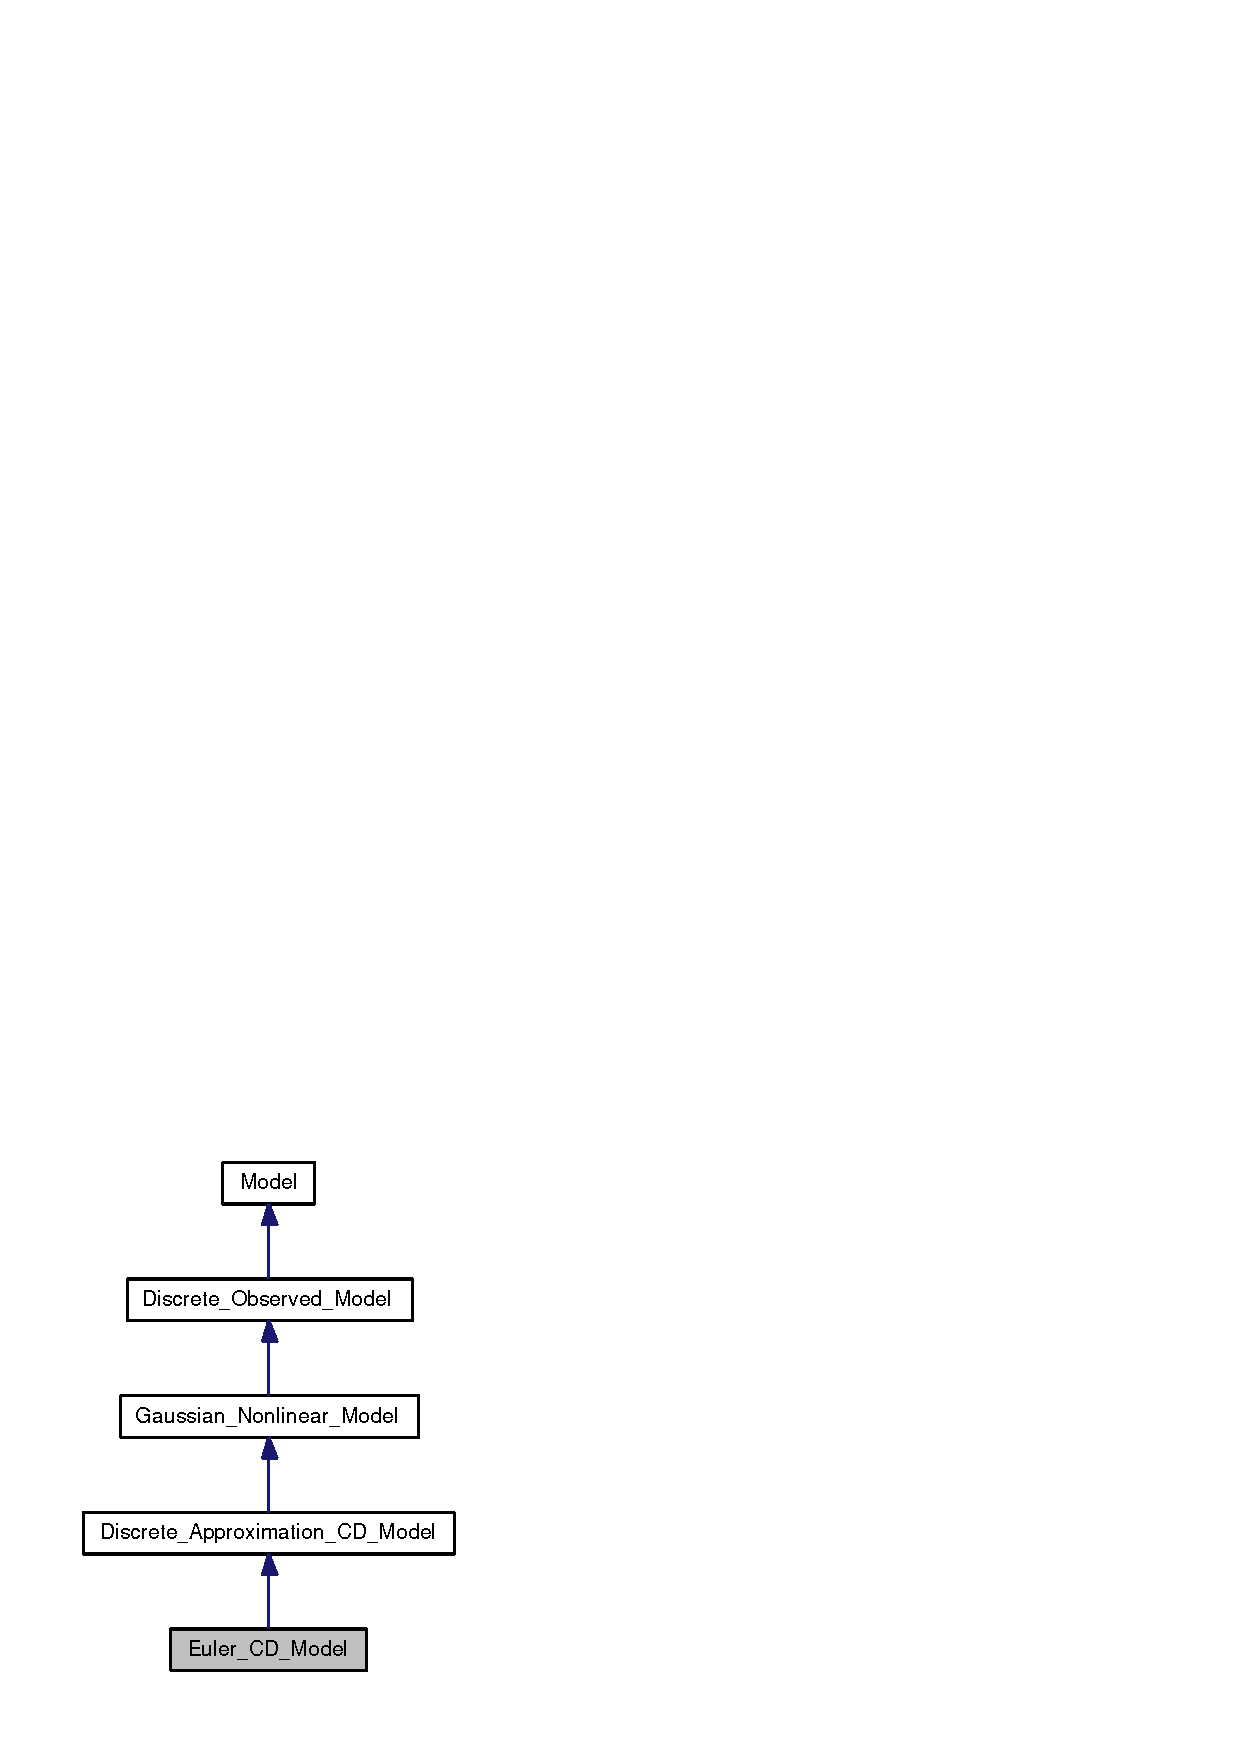
\includegraphics[width=111pt]{class_euler___c_d___model__inherit__graph}
\end{center}
\end{figure}
\subsection*{Public Member Functions}
\begin{CompactItemize}
\item 
\hyperlink{class_euler___c_d___model_10ce5994cf0e94c995e39984ca7d5839}{Euler\_\-CD\_\-Model} (void)
\item 
\hyperlink{class_euler___c_d___model_ca92bef525ab4e38db0cdd66f1ad34fd}{Euler\_\-CD\_\-Model} (\hyperlink{class_continuous___discrete___model}{Continuous\_\-Discrete\_\-Model} $\ast$m, const int \&a)
\item 
dcovector \hyperlink{class_euler___c_d___model_c113d0fdd6ba262f11ddfc0446827469}{Scheme} (const dcovector \&X, const dcovector \&W)
\item 
void \hyperlink{class_euler___c_d___model_e67b3130695db99e6057811914994aed}{Get\_\-Linear\_\-Scheme} (const dcovector \&X, const dcovector \&W, dgematrix \&F, dgematrix \&J, dcovector \&Xp)
\begin{CompactList}\small\item\em Get the Linearized parameters Scheme in X,W. \item\end{CompactList}\item 
dgematrix \hyperlink{class_euler___c_d___model_31ea181a55cb1b348bd483f5fe077c50}{Jx\_\-Scheme} (const dcovector \&X, const dcovector \&W)
\item 
dgematrix \hyperlink{class_euler___c_d___model_d4b9cef601904d1e86c2f3a5f9e01b06}{Jw\_\-Scheme} (const dcovector \&X, const dcovector \&W)
\end{CompactItemize}


\subsection{Detailed Description}
continuous discret model: the state SDE is discretly approximate by an Euler method 

\subsection{Constructor \& Destructor Documentation}
\hypertarget{class_euler___c_d___model_10ce5994cf0e94c995e39984ca7d5839}{
\index{Euler\_\-CD\_\-Model@{Euler\_\-CD\_\-Model}!Euler\_\-CD\_\-Model@{Euler\_\-CD\_\-Model}}
\index{Euler\_\-CD\_\-Model@{Euler\_\-CD\_\-Model}!Euler_CD_Model@{Euler\_\-CD\_\-Model}}
\subsubsection[{Euler\_\-CD\_\-Model}]{\setlength{\rightskip}{0pt plus 5cm}Euler\_\-CD\_\-Model::Euler\_\-CD\_\-Model (void)}}
\label{class_euler___c_d___model_10ce5994cf0e94c995e39984ca7d5839}


\hypertarget{class_euler___c_d___model_ca92bef525ab4e38db0cdd66f1ad34fd}{
\index{Euler\_\-CD\_\-Model@{Euler\_\-CD\_\-Model}!Euler\_\-CD\_\-Model@{Euler\_\-CD\_\-Model}}
\index{Euler\_\-CD\_\-Model@{Euler\_\-CD\_\-Model}!Euler_CD_Model@{Euler\_\-CD\_\-Model}}
\subsubsection[{Euler\_\-CD\_\-Model}]{\setlength{\rightskip}{0pt plus 5cm}Euler\_\-CD\_\-Model::Euler\_\-CD\_\-Model ({\bf Continuous\_\-Discrete\_\-Model} $\ast$ {\em m}, \/  const int \& {\em a})}}
\label{class_euler___c_d___model_ca92bef525ab4e38db0cdd66f1ad34fd}




\subsection{Member Function Documentation}
\hypertarget{class_euler___c_d___model_e67b3130695db99e6057811914994aed}{
\index{Euler\_\-CD\_\-Model@{Euler\_\-CD\_\-Model}!Get\_\-Linear\_\-Scheme@{Get\_\-Linear\_\-Scheme}}
\index{Get\_\-Linear\_\-Scheme@{Get\_\-Linear\_\-Scheme}!Euler_CD_Model@{Euler\_\-CD\_\-Model}}
\subsubsection[{Get\_\-Linear\_\-Scheme}]{\setlength{\rightskip}{0pt plus 5cm}void Euler\_\-CD\_\-Model::Get\_\-Linear\_\-Scheme (const dcovector \& {\em X}, \/  const dcovector \& {\em W}, \/  dgematrix \& {\em F}, \/  dgematrix \& {\em J}, \/  dcovector \& {\em Xp})\hspace{0.3cm}{\tt  \mbox{[}virtual\mbox{]}}}}
\label{class_euler___c_d___model_e67b3130695db99e6057811914994aed}


Get the Linearized parameters Scheme in X,W. 

\begin{Desc}
\item[Parameters:]
\begin{description}
\item[{\em X}]The state value \item[{\em W}]The noise value \item[{\em F}]The jacobian of f(X,W) in X \item[{\em G}]The jacobian in f(X,W) in W \item[{\em Xp}]The prediction Xp = f(X,W) \end{description}
\end{Desc}


Implements \hyperlink{class_discrete___approximation___c_d___model_0a486fada10e6f5569d186edc7b32110}{Discrete\_\-Approximation\_\-CD\_\-Model}.\hypertarget{class_euler___c_d___model_d4b9cef601904d1e86c2f3a5f9e01b06}{
\index{Euler\_\-CD\_\-Model@{Euler\_\-CD\_\-Model}!Jw\_\-Scheme@{Jw\_\-Scheme}}
\index{Jw\_\-Scheme@{Jw\_\-Scheme}!Euler_CD_Model@{Euler\_\-CD\_\-Model}}
\subsubsection[{Jw\_\-Scheme}]{\setlength{\rightskip}{0pt plus 5cm}dgematrix Euler\_\-CD\_\-Model::Jw\_\-Scheme (const dcovector \& {\em X}, \/  const dcovector \& {\em W})\hspace{0.3cm}{\tt  \mbox{[}virtual\mbox{]}}}}
\label{class_euler___c_d___model_d4b9cef601904d1e86c2f3a5f9e01b06}




Implements \hyperlink{class_discrete___approximation___c_d___model_c7496999409a3f05125ceb7fe85e85ab}{Discrete\_\-Approximation\_\-CD\_\-Model}.\hypertarget{class_euler___c_d___model_31ea181a55cb1b348bd483f5fe077c50}{
\index{Euler\_\-CD\_\-Model@{Euler\_\-CD\_\-Model}!Jx\_\-Scheme@{Jx\_\-Scheme}}
\index{Jx\_\-Scheme@{Jx\_\-Scheme}!Euler_CD_Model@{Euler\_\-CD\_\-Model}}
\subsubsection[{Jx\_\-Scheme}]{\setlength{\rightskip}{0pt plus 5cm}dgematrix Euler\_\-CD\_\-Model::Jx\_\-Scheme (const dcovector \& {\em X}, \/  const dcovector \& {\em W})\hspace{0.3cm}{\tt  \mbox{[}virtual\mbox{]}}}}
\label{class_euler___c_d___model_31ea181a55cb1b348bd483f5fe077c50}




Implements \hyperlink{class_discrete___approximation___c_d___model_7a3dcae055d90be0b8a231eff961e2a2}{Discrete\_\-Approximation\_\-CD\_\-Model}.\hypertarget{class_euler___c_d___model_c113d0fdd6ba262f11ddfc0446827469}{
\index{Euler\_\-CD\_\-Model@{Euler\_\-CD\_\-Model}!Scheme@{Scheme}}
\index{Scheme@{Scheme}!Euler_CD_Model@{Euler\_\-CD\_\-Model}}
\subsubsection[{Scheme}]{\setlength{\rightskip}{0pt plus 5cm}dcovector Euler\_\-CD\_\-Model::Scheme (const dcovector \& {\em X}, \/  const dcovector \& {\em W})\hspace{0.3cm}{\tt  \mbox{[}virtual\mbox{]}}}}
\label{class_euler___c_d___model_c113d0fdd6ba262f11ddfc0446827469}




Implements \hyperlink{class_discrete___approximation___c_d___model_1ea9a1d618890fc51db6fa98eeb7af7f}{Discrete\_\-Approximation\_\-CD\_\-Model}.
\hypertarget{class_extended___kalman___filter}{
\section{Extended\_\-Kalman\_\-Filter Class Reference}
\label{class_extended___kalman___filter}\index{Extended\_\-Kalman\_\-Filter@{Extended\_\-Kalman\_\-Filter}}
}
{\tt \#include $<$extended\_\-kalman\_\-filter.h$>$}

Inheritance diagram for Extended\_\-Kalman\_\-Filter:\nopagebreak
\begin{figure}[H]
\begin{center}
\leavevmode
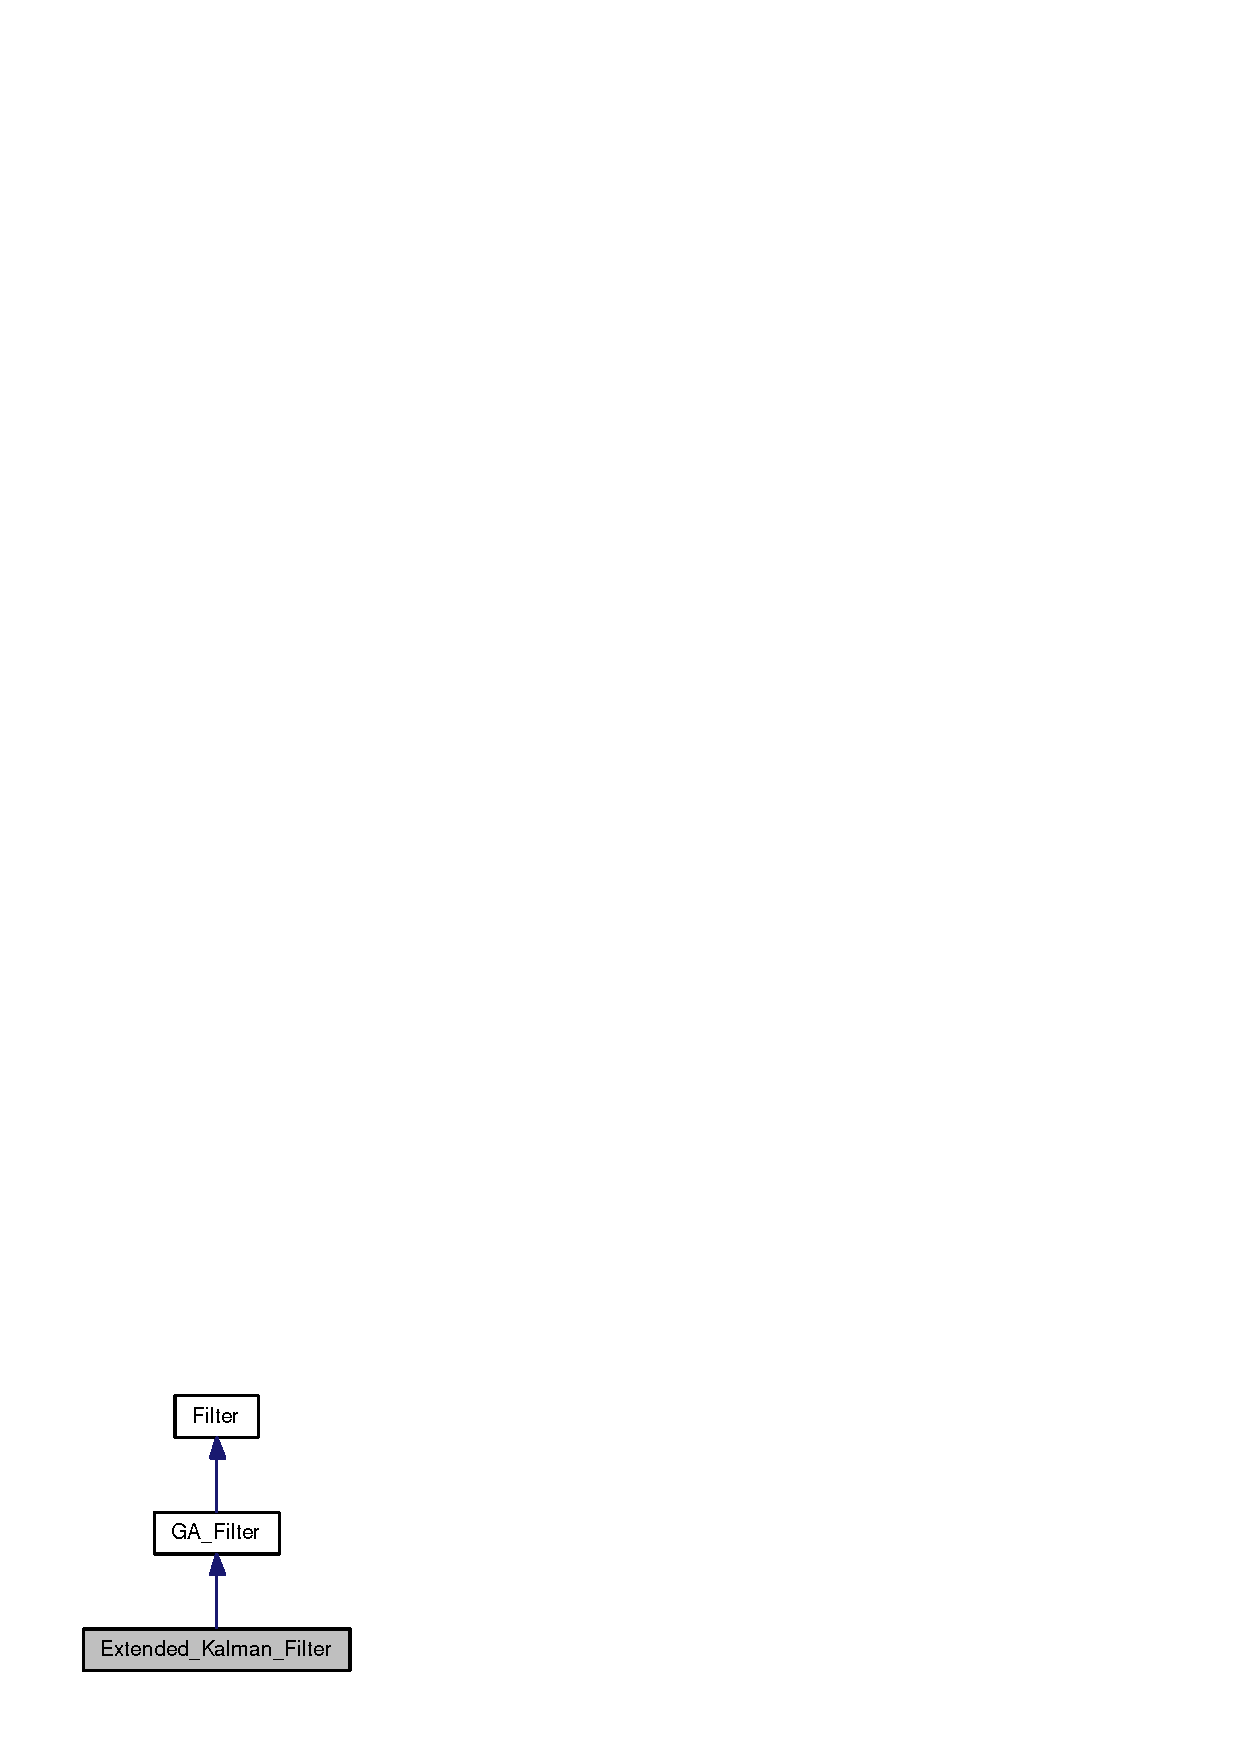
\includegraphics[width=86pt]{class_extended___kalman___filter__inherit__graph}
\end{center}
\end{figure}
\subsection*{Public Member Functions}
\begin{CompactItemize}
\item 
\hyperlink{class_extended___kalman___filter_faec3e417aa36543328924021abd2bd1}{Extended\_\-Kalman\_\-Filter} (void)
\item 
\hyperlink{class_extended___kalman___filter_e236e49f87357c4e2958c885fd667092}{Extended\_\-Kalman\_\-Filter} (\hyperlink{class_gaussian___nonlinear___model}{Gaussian\_\-Nonlinear\_\-Model} $\ast$m)
\end{CompactItemize}
\subsection*{Protected Member Functions}
\begin{CompactItemize}
\item 
int \hyperlink{class_extended___kalman___filter_5cfabc6d2256b22baca0a908d29c9c7e}{\_\-update} (const dcovector \&Y)
\end{CompactItemize}


\subsection{Constructor \& Destructor Documentation}
\hypertarget{class_extended___kalman___filter_faec3e417aa36543328924021abd2bd1}{
\index{Extended\_\-Kalman\_\-Filter@{Extended\_\-Kalman\_\-Filter}!Extended\_\-Kalman\_\-Filter@{Extended\_\-Kalman\_\-Filter}}
\index{Extended\_\-Kalman\_\-Filter@{Extended\_\-Kalman\_\-Filter}!Extended_Kalman_Filter@{Extended\_\-Kalman\_\-Filter}}
\subsubsection[{Extended\_\-Kalman\_\-Filter}]{\setlength{\rightskip}{0pt plus 5cm}Extended\_\-Kalman\_\-Filter::Extended\_\-Kalman\_\-Filter (void)}}
\label{class_extended___kalman___filter_faec3e417aa36543328924021abd2bd1}


\hypertarget{class_extended___kalman___filter_e236e49f87357c4e2958c885fd667092}{
\index{Extended\_\-Kalman\_\-Filter@{Extended\_\-Kalman\_\-Filter}!Extended\_\-Kalman\_\-Filter@{Extended\_\-Kalman\_\-Filter}}
\index{Extended\_\-Kalman\_\-Filter@{Extended\_\-Kalman\_\-Filter}!Extended_Kalman_Filter@{Extended\_\-Kalman\_\-Filter}}
\subsubsection[{Extended\_\-Kalman\_\-Filter}]{\setlength{\rightskip}{0pt plus 5cm}Extended\_\-Kalman\_\-Filter::Extended\_\-Kalman\_\-Filter ({\bf Gaussian\_\-Nonlinear\_\-Model} $\ast$ {\em m})}}
\label{class_extended___kalman___filter_e236e49f87357c4e2958c885fd667092}




\subsection{Member Function Documentation}
\hypertarget{class_extended___kalman___filter_5cfabc6d2256b22baca0a908d29c9c7e}{
\index{Extended\_\-Kalman\_\-Filter@{Extended\_\-Kalman\_\-Filter}!\_\-update@{\_\-update}}
\index{\_\-update@{\_\-update}!Extended_Kalman_Filter@{Extended\_\-Kalman\_\-Filter}}
\subsubsection[{\_\-update}]{\setlength{\rightskip}{0pt plus 5cm}int Extended\_\-Kalman\_\-Filter::\_\-update (const dcovector \& {\em Y})\hspace{0.3cm}{\tt  \mbox{[}protected, virtual\mbox{]}}}}
\label{class_extended___kalman___filter_5cfabc6d2256b22baca0a908d29c9c7e}


Specific update for each filter

\begin{Desc}
\item[Parameters:]
\begin{description}
\item[{\em Y}]The observed sample\end{description}
\end{Desc}
\begin{Desc}
\item[Returns:]0 if no problem \end{Desc}


Implements \hyperlink{class_filter_20ecd17fed3b8f11a76c960fe5e7144b}{Filter}.
\hypertarget{class_filter}{
\section{Filter Class Reference}
\label{class_filter}\index{Filter@{Filter}}
}
Abstract class of all filters.  


{\tt \#include $<$filter.h$>$}

Inheritance diagram for Filter:\nopagebreak
\begin{figure}[H]
\begin{center}
\leavevmode
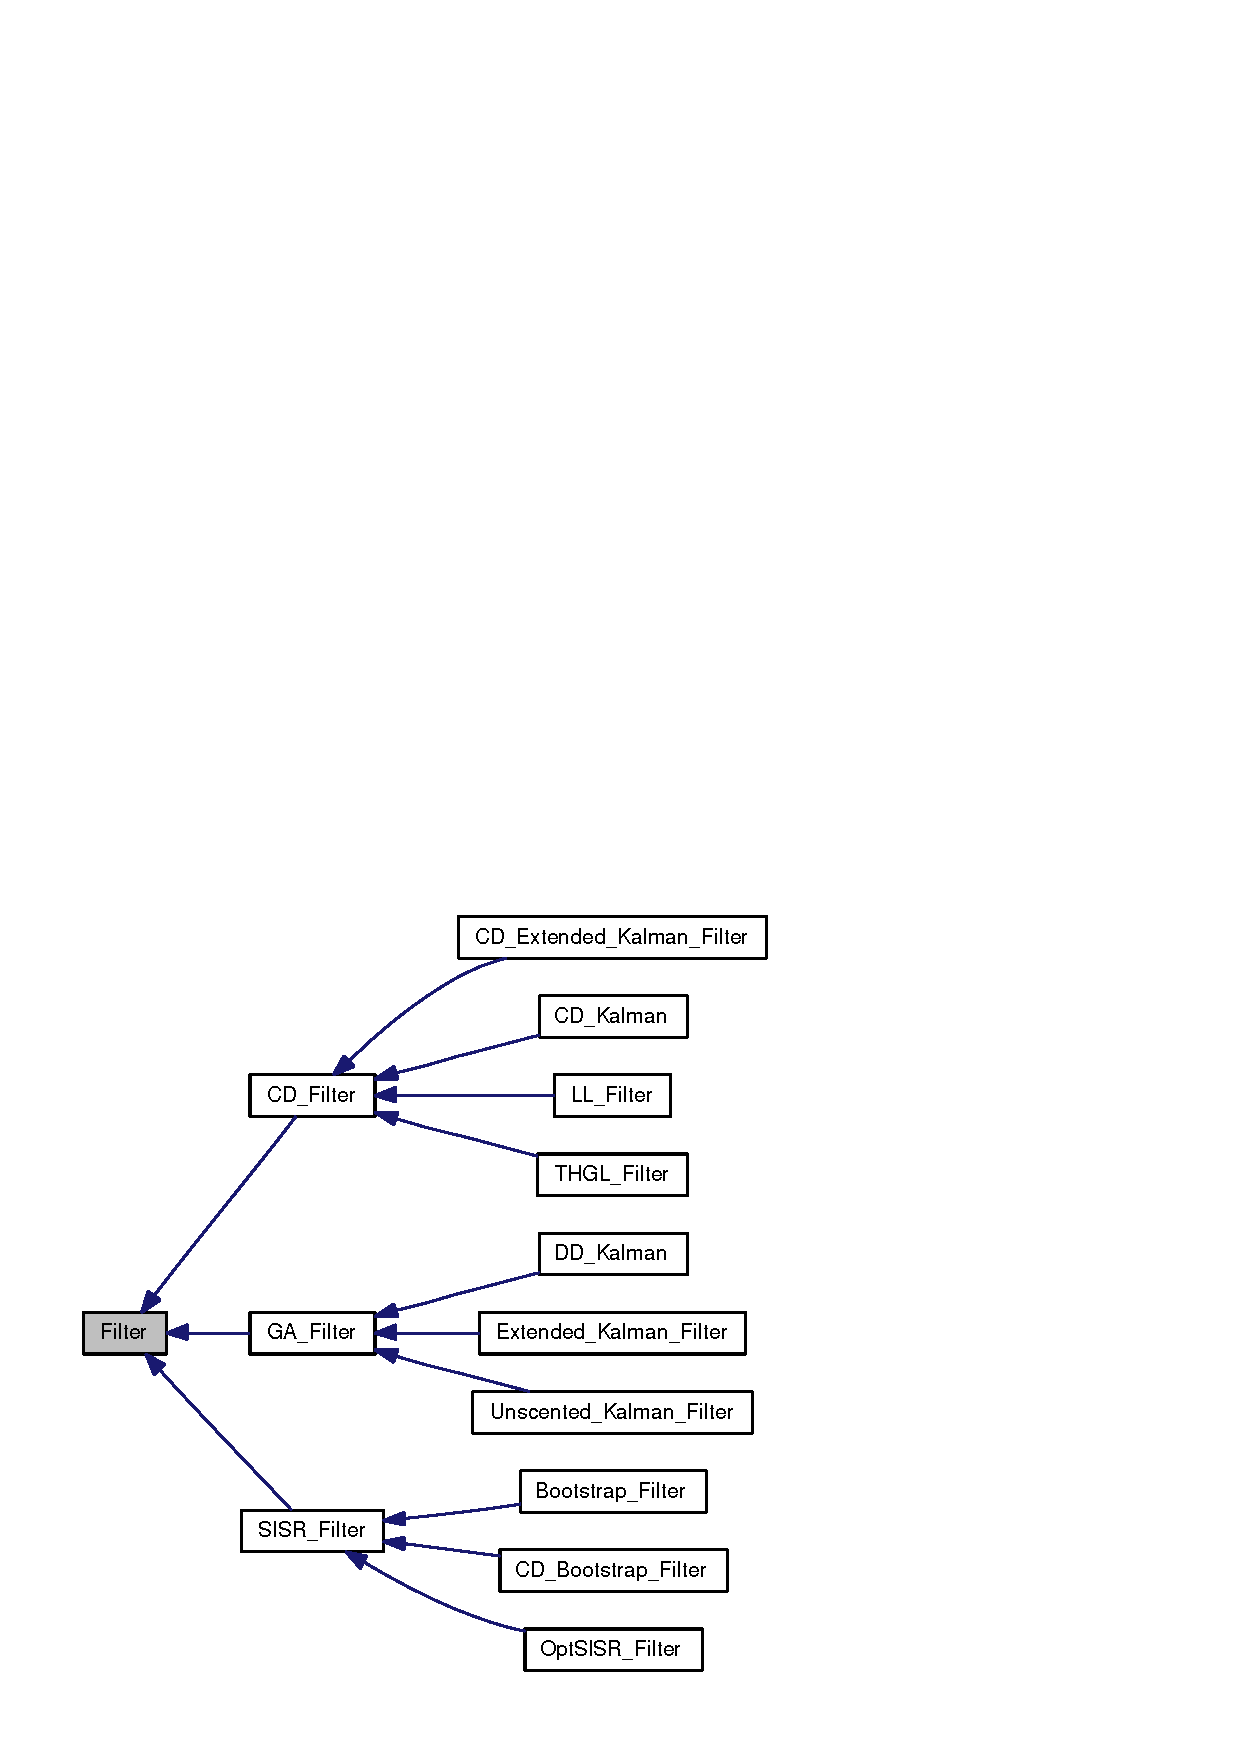
\includegraphics[height=400pt]{class_filter__inherit__graph}
\end{center}
\end{figure}
\subsection*{Public Member Functions}
\begin{CompactItemize}
\item 
\hyperlink{class_filter_b86c90163e27f662edd126f5ae0d0334}{Filter} (void)
\item 
virtual \hyperlink{class_filter_f8a7766f99dd11bc8d02033e7be95c38}{$\sim$Filter} (void)
\item 
int \hyperlink{class_filter_75ba779211698e81a2334a568dcba76e}{Update} (const dcovector \&Y)
\item 
int \hyperlink{class_filter_d7944eca3250087246371a2f77e50f87}{Filtering} (const vector$<$ dcovector $>$ \&Y)
\item 
virtual dcovector \hyperlink{class_filter_f6e41ec8ada47571291b31a259858cdc}{Expected\_\-Get} (void)=0
\item 
int \hyperlink{class_filter_fbfb19e91e31f29cdcef04b9fa48c466}{Init} (void)
\item 
double \hyperlink{class_filter_0dd24e89e97c71dd06766483734c1f2a}{Likelihood\_\-Get} (void)
\item 
virtual int \hyperlink{class_filter_0b7aad4b130b176f423b7f1c0c30a887}{Save\_\-X} (const char $\ast$filename)
\end{CompactItemize}
\subsection*{Public Attributes}
\begin{CompactItemize}
\item 
\hyperlink{class_model}{Model} $\ast$ \hyperlink{class_filter_2173d25727b871e9b9d0b6f588ba3cd2}{model}
\begin{CompactList}\small\item\em The hidden markov model. \item\end{CompactList}\item 
vector$<$ dcovector $>$ \hyperlink{class_filter_fc564c7effa729f11710d78ae0111ec1}{X}
\begin{CompactList}\small\item\em $ \{ \hat{X}_{k|k} ,k=0,...N \} $ \item\end{CompactList}\end{CompactItemize}
\subsection*{Protected Member Functions}
\begin{CompactItemize}
\item 
virtual int \hyperlink{class_filter_20ecd17fed3b8f11a76c960fe5e7144b}{\_\-update} (const dcovector \&Y)=0
\item 
virtual int \hyperlink{class_filter_f46a456184971270ca36733d937f14fb}{\_\-init} (void)=0
\end{CompactItemize}
\subsection*{Protected Attributes}
\begin{CompactItemize}
\item 
double \hyperlink{class_filter_5d4fd0aac4fddb732fc42e680fab5a1f}{Likelihood}
\begin{CompactList}\small\item\em The likelihood $ p_{Y_{0:N}}(y_{0:N}) $. \item\end{CompactList}\end{CompactItemize}


\subsection{Detailed Description}
Abstract class of all filters. 

Filters calculate recursively an estimation $ \hat{X}_{k|k} $ of the STATE $ X_{k} $ of a hidden markov model (\hyperlink{class_model}{Model}) given observations $ Y_{0:k} $. \begin{Desc}
\item[]\end{Desc}
They compute also recursively the likelihood $ p_{Y_{0:N}}(y_{0:N}) $. 

\subsection{Constructor \& Destructor Documentation}
\hypertarget{class_filter_b86c90163e27f662edd126f5ae0d0334}{
\index{Filter@{Filter}!Filter@{Filter}}
\index{Filter@{Filter}!Filter@{Filter}}
\subsubsection[{Filter}]{\setlength{\rightskip}{0pt plus 5cm}Filter::Filter (void)}}
\label{class_filter_b86c90163e27f662edd126f5ae0d0334}


A constructor \hypertarget{class_filter_f8a7766f99dd11bc8d02033e7be95c38}{
\index{Filter@{Filter}!$\sim$Filter@{$\sim$Filter}}
\index{$\sim$Filter@{$\sim$Filter}!Filter@{Filter}}
\subsubsection[{$\sim$Filter}]{\setlength{\rightskip}{0pt plus 5cm}virtual Filter::$\sim$Filter (void)\hspace{0.3cm}{\tt  \mbox{[}virtual\mbox{]}}}}
\label{class_filter_f8a7766f99dd11bc8d02033e7be95c38}


The destructor 

\subsection{Member Function Documentation}
\hypertarget{class_filter_f46a456184971270ca36733d937f14fb}{
\index{Filter@{Filter}!\_\-init@{\_\-init}}
\index{\_\-init@{\_\-init}!Filter@{Filter}}
\subsubsection[{\_\-init}]{\setlength{\rightskip}{0pt plus 5cm}virtual int Filter::\_\-init (void)\hspace{0.3cm}{\tt  \mbox{[}protected, pure virtual\mbox{]}}}}
\label{class_filter_f46a456184971270ca36733d937f14fb}


Specific init for each filter

\begin{Desc}
\item[Parameters:]
\begin{description}
\item[{\em Y}]The observed sample\end{description}
\end{Desc}
\begin{Desc}
\item[Returns:]0 if no problem \end{Desc}


Implemented in \hyperlink{class_g_a___filter_7b5cb872bcedd752a4309f114625a4b8}{GA\_\-Filter}, \hyperlink{class_c_d___filter_789c745e24ee5534d22455dff70a93b3}{CD\_\-Filter}, \hyperlink{class_s_i_s_r___filter_307c7a9012848bb6d441020443191725}{SISR\_\-Filter}, and \hyperlink{class_unscented___kalman___filter_a6ca6d9f8b5a4a40c18b6cdfdc2029fa}{Unscented\_\-Kalman\_\-Filter}.\hypertarget{class_filter_20ecd17fed3b8f11a76c960fe5e7144b}{
\index{Filter@{Filter}!\_\-update@{\_\-update}}
\index{\_\-update@{\_\-update}!Filter@{Filter}}
\subsubsection[{\_\-update}]{\setlength{\rightskip}{0pt plus 5cm}virtual int Filter::\_\-update (const dcovector \& {\em Y})\hspace{0.3cm}{\tt  \mbox{[}protected, pure virtual\mbox{]}}}}
\label{class_filter_20ecd17fed3b8f11a76c960fe5e7144b}


Specific update for each filter

\begin{Desc}
\item[Parameters:]
\begin{description}
\item[{\em Y}]The observed sample\end{description}
\end{Desc}
\begin{Desc}
\item[Returns:]0 if no problem \end{Desc}


Implemented in \hyperlink{class_extended___kalman___filter_5cfabc6d2256b22baca0a908d29c9c7e}{Extended\_\-Kalman\_\-Filter}, \hyperlink{class_c_d___extended___kalman___filter_7cfd2bf966970f44f4e1480ed3852b69}{CD\_\-Extended\_\-Kalman\_\-Filter}, \hyperlink{class_c_d___kalman_ecef658eac67b1005d9e86ec30708300}{CD\_\-Kalman}, \hyperlink{class_d_d___kalman_a04e9be77c495296673227860833c9fc}{DD\_\-Kalman}, \hyperlink{class_l_l___filter_ab2b4b545d401d54c66f63a41fa1a99d}{LL\_\-Filter}, \hyperlink{class_s_i_s_r___filter_e6aac1c96b9c6803425fd712cbf730d1}{SISR\_\-Filter}, \hyperlink{class_t_h_g_l___filter_2139ff41dc0eaa613847429c266ba7a5}{THGL\_\-Filter}, and \hyperlink{class_unscented___kalman___filter_ee1e0a8035111d7695b6958c644f97cc}{Unscented\_\-Kalman\_\-Filter}.\hypertarget{class_filter_f6e41ec8ada47571291b31a259858cdc}{
\index{Filter@{Filter}!Expected\_\-Get@{Expected\_\-Get}}
\index{Expected\_\-Get@{Expected\_\-Get}!Filter@{Filter}}
\subsubsection[{Expected\_\-Get}]{\setlength{\rightskip}{0pt plus 5cm}virtual dcovector Filter::Expected\_\-Get (void)\hspace{0.3cm}{\tt  \mbox{[}pure virtual\mbox{]}}}}
\label{class_filter_f6e41ec8ada47571291b31a259858cdc}


Evaluate the current estimation of the state

\begin{Desc}
\item[Returns:]$ \hat{X}_{k|k} $ \end{Desc}


Implemented in \hyperlink{class_g_a___filter_e92898cc15e34358cb9ecabd57067a39}{GA\_\-Filter}, \hyperlink{class_c_d___filter_f5c2b82877e5cdad1e0cc782374809b0}{CD\_\-Filter}, and \hyperlink{class_s_i_s_r___filter_2d1eb0ceb62531ed48af9a424bc62210}{SISR\_\-Filter}.\hypertarget{class_filter_d7944eca3250087246371a2f77e50f87}{
\index{Filter@{Filter}!Filtering@{Filtering}}
\index{Filtering@{Filtering}!Filter@{Filter}}
\subsubsection[{Filtering}]{\setlength{\rightskip}{0pt plus 5cm}int Filter::Filtering (const vector$<$ dcovector $>$ \& {\em Y})}}
\label{class_filter_d7944eca3250087246371a2f77e50f87}


Perform a trajectory state estimation given a sequence $ y_{0:N}$

\begin{Desc}
\item[Parameters:]
\begin{description}
\item[{\em Y}]The sequence\end{description}
\end{Desc}
\begin{Desc}
\item[Returns:]0 if everything is ok \end{Desc}
\hypertarget{class_filter_fbfb19e91e31f29cdcef04b9fa48c466}{
\index{Filter@{Filter}!Init@{Init}}
\index{Init@{Init}!Filter@{Filter}}
\subsubsection[{Init}]{\setlength{\rightskip}{0pt plus 5cm}int Filter::Init (void)}}
\label{class_filter_fbfb19e91e31f29cdcef04b9fa48c466}


To init the filter at k=0 \hypertarget{class_filter_0dd24e89e97c71dd06766483734c1f2a}{
\index{Filter@{Filter}!Likelihood\_\-Get@{Likelihood\_\-Get}}
\index{Likelihood\_\-Get@{Likelihood\_\-Get}!Filter@{Filter}}
\subsubsection[{Likelihood\_\-Get}]{\setlength{\rightskip}{0pt plus 5cm}double Filter::Likelihood\_\-Get (void)}}
\label{class_filter_0dd24e89e97c71dd06766483734c1f2a}


Return the current likelihood $ p_{Y_{0:k}}(y_{0:k}) $

\begin{Desc}
\item[Returns:]$ p_{Y_{0:N}}(y_{0:N}) $ \end{Desc}
\hypertarget{class_filter_0b7aad4b130b176f423b7f1c0c30a887}{
\index{Filter@{Filter}!Save\_\-X@{Save\_\-X}}
\index{Save\_\-X@{Save\_\-X}!Filter@{Filter}}
\subsubsection[{Save\_\-X}]{\setlength{\rightskip}{0pt plus 5cm}virtual int Filter::Save\_\-X (const char $\ast$ {\em filename})\hspace{0.3cm}{\tt  \mbox{[}virtual\mbox{]}}}}
\label{class_filter_0b7aad4b130b176f423b7f1c0c30a887}


Save the estimation $ \{ \hat{X}_{k|k} ,k=0,...N \} $

\begin{Desc}
\item[Parameters:]
\begin{description}
\item[{\em filename}]\end{description}
\end{Desc}
\begin{Desc}
\item[Returns:]0 if everything is ok \end{Desc}


Reimplemented in \hyperlink{class_c_d___filter_b304de0cc156193c9e938188c1092188}{CD\_\-Filter}, and \hyperlink{class_c_d___bootstrap___filter_eb203b8cdeb51133a232dce5763ed153}{CD\_\-Bootstrap\_\-Filter}.\hypertarget{class_filter_75ba779211698e81a2334a568dcba76e}{
\index{Filter@{Filter}!Update@{Update}}
\index{Update@{Update}!Filter@{Filter}}
\subsubsection[{Update}]{\setlength{\rightskip}{0pt plus 5cm}int Filter::Update (const dcovector \& {\em Y})}}
\label{class_filter_75ba779211698e81a2334a568dcba76e}


Perform an estimation step with a new observation

\begin{Desc}
\item[Parameters:]
\begin{description}
\item[{\em Y}]The new observed sample\end{description}
\end{Desc}
\begin{Desc}
\item[Returns:]0 if everything is ok \end{Desc}


\subsection{Member Data Documentation}
\hypertarget{class_filter_5d4fd0aac4fddb732fc42e680fab5a1f}{
\index{Filter@{Filter}!Likelihood@{Likelihood}}
\index{Likelihood@{Likelihood}!Filter@{Filter}}
\subsubsection[{Likelihood}]{\setlength{\rightskip}{0pt plus 5cm}double {\bf Filter::Likelihood}\hspace{0.3cm}{\tt  \mbox{[}protected\mbox{]}}}}
\label{class_filter_5d4fd0aac4fddb732fc42e680fab5a1f}


The likelihood $ p_{Y_{0:N}}(y_{0:N}) $. 

\hypertarget{class_filter_2173d25727b871e9b9d0b6f588ba3cd2}{
\index{Filter@{Filter}!model@{model}}
\index{model@{model}!Filter@{Filter}}
\subsubsection[{model}]{\setlength{\rightskip}{0pt plus 5cm}{\bf Model}$\ast$ {\bf Filter::model}}}
\label{class_filter_2173d25727b871e9b9d0b6f588ba3cd2}


The hidden markov model. 

\hypertarget{class_filter_fc564c7effa729f11710d78ae0111ec1}{
\index{Filter@{Filter}!X@{X}}
\index{X@{X}!Filter@{Filter}}
\subsubsection[{X}]{\setlength{\rightskip}{0pt plus 5cm}vector$<$dcovector$>$ {\bf Filter::X}}}
\label{class_filter_fc564c7effa729f11710d78ae0111ec1}


$ \{ \hat{X}_{k|k} ,k=0,...N \} $ 

The estimated trajectory of the state 
\hypertarget{class_g___simulator}{
\section{G\_\-Simulator Class Reference}
\label{class_g___simulator}\index{G\_\-Simulator@{G\_\-Simulator}}
}
{\tt \#include $<$simulator.h$>$}

Inheritance diagram for G\_\-Simulator:\nopagebreak
\begin{figure}[H]
\begin{center}
\leavevmode
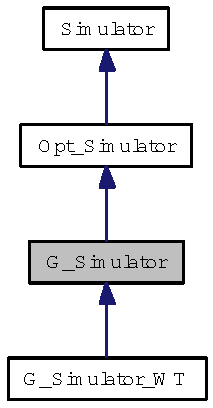
\includegraphics[width=69pt]{class_g___simulator__inherit__graph}
\end{center}
\end{figure}
\subsection*{Public Member Functions}
\begin{CompactItemize}
\item 
\hyperlink{class_g___simulator_f73fe624aee09a345b153b9c2fe7a8a5}{G\_\-Simulator} (void)
\item 
\hyperlink{class_g___simulator_a42df6b23b83676a63e0afb6e765ea5e}{G\_\-Simulator} (\hyperlink{class_gaussian___nonlinear___model}{Gaussian\_\-Nonlinear\_\-Model} $\ast$m)
\item 
dcovector \hyperlink{class_g___simulator_0e9a1d220c5457cc07c6bcdb70e1638c}{Draw\_\-Init} (void)
\begin{CompactList}\small\item\em Draw a sample from p(X0). \item\end{CompactList}\item 
dcovector \hyperlink{class_g___simulator_54563826e17b08d4cf66090731797888}{Draw\_\-Transition} (const dcovector \&Xkm1)
\begin{CompactList}\small\item\em Draw a sample from the transition densisty p(Xk$|$Xk-1). \item\end{CompactList}\item 
dcovector \hyperlink{class_g___simulator_b53bc573683cef16a5117dcc71a1f0a7}{Draw\_\-Observation} (const dcovector \&Xk)
\begin{CompactList}\small\item\em Calculate the value of the density of probability of Y given X : p(Y$|$X). \item\end{CompactList}\item 
long double \hyperlink{class_g___simulator_6f42783322c20a0b91fab9f1e6d54363}{Observation\_\-Density} (const dcovector \&\hyperlink{class_simulator_403a127c909abf3e4c6d48a287315987}{Y}, const dcovector \&\hyperlink{class_simulator_a2db8ace19099d996be516022d230bc0}{X})
\begin{CompactList}\small\item\em calculate the value of the density of probability of Y given X : p(Y$|$X) \item\end{CompactList}\item 
dcovector \hyperlink{class_g___simulator_b6c78e1dfa62c8c684b860ea1918f045}{Draw\_\-Optimal} (const dcovector \&Yk, const dcovector \&Xkm1)
\begin{CompactList}\small\item\em Draw a sample from the optimal densisty p(Xk$|$Yk,Xk-1). \item\end{CompactList}\item 
long double \hyperlink{class_g___simulator_192df25d6edac87bf4aeb2d2f55d1c5c}{Obs\_\-Optimal\_\-Density} (const dcovector \&Yk, const dcovector \&Xkm1)
\begin{CompactList}\small\item\em calculate the value of the density of probability of Yk given Xk-1 : p(Yk$|$Xk-1) \item\end{CompactList}\end{CompactItemize}


\subsection{Constructor \& Destructor Documentation}
\hypertarget{class_g___simulator_f73fe624aee09a345b153b9c2fe7a8a5}{
\index{G\_\-Simulator@{G\_\-Simulator}!G\_\-Simulator@{G\_\-Simulator}}
\index{G\_\-Simulator@{G\_\-Simulator}!G_Simulator@{G\_\-Simulator}}
\subsubsection[{G\_\-Simulator}]{\setlength{\rightskip}{0pt plus 5cm}G\_\-Simulator::G\_\-Simulator (void)}}
\label{class_g___simulator_f73fe624aee09a345b153b9c2fe7a8a5}


\hypertarget{class_g___simulator_a42df6b23b83676a63e0afb6e765ea5e}{
\index{G\_\-Simulator@{G\_\-Simulator}!G\_\-Simulator@{G\_\-Simulator}}
\index{G\_\-Simulator@{G\_\-Simulator}!G_Simulator@{G\_\-Simulator}}
\subsubsection[{G\_\-Simulator}]{\setlength{\rightskip}{0pt plus 5cm}G\_\-Simulator::G\_\-Simulator ({\bf Gaussian\_\-Nonlinear\_\-Model} $\ast$ {\em m})}}
\label{class_g___simulator_a42df6b23b83676a63e0afb6e765ea5e}




\subsection{Member Function Documentation}
\hypertarget{class_g___simulator_0e9a1d220c5457cc07c6bcdb70e1638c}{
\index{G\_\-Simulator@{G\_\-Simulator}!Draw\_\-Init@{Draw\_\-Init}}
\index{Draw\_\-Init@{Draw\_\-Init}!G_Simulator@{G\_\-Simulator}}
\subsubsection[{Draw\_\-Init}]{\setlength{\rightskip}{0pt plus 5cm}dcovector G\_\-Simulator::Draw\_\-Init (void)\hspace{0.3cm}{\tt  \mbox{[}virtual\mbox{]}}}}
\label{class_g___simulator_0e9a1d220c5457cc07c6bcdb70e1638c}


Draw a sample from p(X0). 

\begin{Desc}
\item[Returns:]A sample from p(X0) \end{Desc}


Implements \hyperlink{class_simulator_29b9603eb2be9139972816329e8663dc}{Simulator}.

Reimplemented in \hyperlink{class_g___simulator___w_t_4dab061e25ad9b7b6c279d65ea3038d2}{G\_\-Simulator\_\-WT}.\hypertarget{class_g___simulator_b53bc573683cef16a5117dcc71a1f0a7}{
\index{G\_\-Simulator@{G\_\-Simulator}!Draw\_\-Observation@{Draw\_\-Observation}}
\index{Draw\_\-Observation@{Draw\_\-Observation}!G_Simulator@{G\_\-Simulator}}
\subsubsection[{Draw\_\-Observation}]{\setlength{\rightskip}{0pt plus 5cm}dcovector G\_\-Simulator::Draw\_\-Observation (const dcovector \& {\em Xk})\hspace{0.3cm}{\tt  \mbox{[}virtual\mbox{]}}}}
\label{class_g___simulator_b53bc573683cef16a5117dcc71a1f0a7}


Calculate the value of the density of probability of Y given X : p(Y$|$X). 

\begin{Desc}
\item[Parameters:]
\begin{description}
\item[{\em Xk}]The state at k\end{description}
\end{Desc}
\begin{Desc}
\item[Returns:]The simulated observation \end{Desc}


Implements \hyperlink{class_simulator_2fb966c2c2a4c93bb6788e15563c9006}{Simulator}.\hypertarget{class_g___simulator_b6c78e1dfa62c8c684b860ea1918f045}{
\index{G\_\-Simulator@{G\_\-Simulator}!Draw\_\-Optimal@{Draw\_\-Optimal}}
\index{Draw\_\-Optimal@{Draw\_\-Optimal}!G_Simulator@{G\_\-Simulator}}
\subsubsection[{Draw\_\-Optimal}]{\setlength{\rightskip}{0pt plus 5cm}dcovector G\_\-Simulator::Draw\_\-Optimal (const dcovector \& {\em Yk}, \/  const dcovector \& {\em Xkm1})\hspace{0.3cm}{\tt  \mbox{[}virtual\mbox{]}}}}
\label{class_g___simulator_b6c78e1dfa62c8c684b860ea1918f045}


Draw a sample from the optimal densisty p(Xk$|$Yk,Xk-1). 

\begin{Desc}
\item[Parameters:]
\begin{description}
\item[{\em Yk}]The obseration at k \item[{\em Xkm1}]X(k-1) the state value at k-1\end{description}
\end{Desc}
\begin{Desc}
\item[Returns:]A sample from the optimal importance density \end{Desc}


Implements \hyperlink{class_opt___simulator_75490247df4dfa14eb7b2d8d394675dd}{Opt\_\-Simulator}.\hypertarget{class_g___simulator_54563826e17b08d4cf66090731797888}{
\index{G\_\-Simulator@{G\_\-Simulator}!Draw\_\-Transition@{Draw\_\-Transition}}
\index{Draw\_\-Transition@{Draw\_\-Transition}!G_Simulator@{G\_\-Simulator}}
\subsubsection[{Draw\_\-Transition}]{\setlength{\rightskip}{0pt plus 5cm}dcovector G\_\-Simulator::Draw\_\-Transition (const dcovector \& {\em Xkm1})\hspace{0.3cm}{\tt  \mbox{[}virtual\mbox{]}}}}
\label{class_g___simulator_54563826e17b08d4cf66090731797888}


Draw a sample from the transition densisty p(Xk$|$Xk-1). 

\begin{Desc}
\item[Parameters:]
\begin{description}
\item[{\em Xkm1}]X(k-1) the preceding state\end{description}
\end{Desc}
\begin{Desc}
\item[Returns:]\end{Desc}


Implements \hyperlink{class_simulator_45790421a1c2f597739d3e972ad28292}{Simulator}.\hypertarget{class_g___simulator_192df25d6edac87bf4aeb2d2f55d1c5c}{
\index{G\_\-Simulator@{G\_\-Simulator}!Obs\_\-Optimal\_\-Density@{Obs\_\-Optimal\_\-Density}}
\index{Obs\_\-Optimal\_\-Density@{Obs\_\-Optimal\_\-Density}!G_Simulator@{G\_\-Simulator}}
\subsubsection[{Obs\_\-Optimal\_\-Density}]{\setlength{\rightskip}{0pt plus 5cm}long double G\_\-Simulator::Obs\_\-Optimal\_\-Density (const dcovector \& {\em Yk}, \/  const dcovector \& {\em Xkm1})\hspace{0.3cm}{\tt  \mbox{[}virtual\mbox{]}}}}
\label{class_g___simulator_192df25d6edac87bf4aeb2d2f55d1c5c}


calculate the value of the density of probability of Yk given Xk-1 : p(Yk$|$Xk-1) 

\begin{Desc}
\item[Parameters:]
\begin{description}
\item[{\em Yk}]the osbervation at k \item[{\em Xkm1}]The state at k-1\end{description}
\end{Desc}
\begin{Desc}
\item[Returns:]The value of the density p(Yk$|$Xk-1) \end{Desc}


Implements \hyperlink{class_opt___simulator_e72d4709998087317635a94c709d71ba}{Opt\_\-Simulator}.\hypertarget{class_g___simulator_6f42783322c20a0b91fab9f1e6d54363}{
\index{G\_\-Simulator@{G\_\-Simulator}!Observation\_\-Density@{Observation\_\-Density}}
\index{Observation\_\-Density@{Observation\_\-Density}!G_Simulator@{G\_\-Simulator}}
\subsubsection[{Observation\_\-Density}]{\setlength{\rightskip}{0pt plus 5cm}long double G\_\-Simulator::Observation\_\-Density (const dcovector \& {\em Y}, \/  const dcovector \& {\em X})\hspace{0.3cm}{\tt  \mbox{[}virtual\mbox{]}}}}
\label{class_g___simulator_6f42783322c20a0b91fab9f1e6d54363}


calculate the value of the density of probability of Y given X : p(Y$|$X) 

\begin{Desc}
\item[Parameters:]
\begin{description}
\item[{\em Y}]The osbervation \item[{\em X}]The state\end{description}
\end{Desc}
\begin{Desc}
\item[Returns:]The value of the density \end{Desc}


Implements \hyperlink{class_simulator_75b0dfb5b0b88346ecb9f7da4fbd91f1}{Simulator}.
\hypertarget{class_g___simulator___w_t}{
\section{G\_\-Simulator\_\-WT Class Reference}
\label{class_g___simulator___w_t}\index{G\_\-Simulator\_\-WT@{G\_\-Simulator\_\-WT}}
}
{\tt \#include $<$simulator.h$>$}

Inheritance diagram for G\_\-Simulator\_\-WT:\nopagebreak
\begin{figure}[H]
\begin{center}
\leavevmode
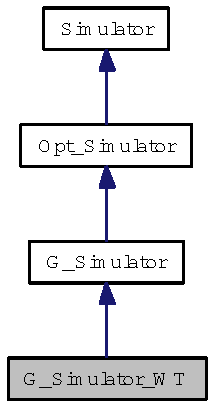
\includegraphics[width=69pt]{class_g___simulator___w_t__inherit__graph}
\end{center}
\end{figure}
\subsection*{Public Member Functions}
\begin{CompactItemize}
\item 
\hyperlink{class_g___simulator___w_t_1d369912b29be6b65bdd0b8ef0769e71}{G\_\-Simulator\_\-WT} (void)
\item 
\hyperlink{class_g___simulator___w_t_307f1d93fda73646944844843d4b53ac}{G\_\-Simulator\_\-WT} (\hyperlink{class_gaussian___nonlinear___model}{Gaussian\_\-Nonlinear\_\-Model} $\ast$m, const int \&\hyperlink{class_g___simulator___w_t_646b6b5a2328052988746ea2e85ec2f5}{NB}, const int \&\hyperlink{class_g___simulator___w_t_8036e2d318c76440f0ed2e23dd5f5523}{N})
\item 
dcovector \hyperlink{class_g___simulator___w_t_4dab061e25ad9b7b6c279d65ea3038d2}{Draw\_\-Init} (void)
\begin{CompactList}\small\item\em Draw a sample from p(X0). \item\end{CompactList}\end{CompactItemize}
\subsection*{Private Attributes}
\begin{CompactItemize}
\item 
vector$<$ dcovector $>$ \hyperlink{class_g___simulator___w_t_74786ef68257c2af89893c9c12a0e7f2}{Xt}
\item 
int \hyperlink{class_g___simulator___w_t_646b6b5a2328052988746ea2e85ec2f5}{NB}
\item 
int \hyperlink{class_g___simulator___w_t_8036e2d318c76440f0ed2e23dd5f5523}{N}
\end{CompactItemize}


\subsection{Constructor \& Destructor Documentation}
\hypertarget{class_g___simulator___w_t_1d369912b29be6b65bdd0b8ef0769e71}{
\index{G\_\-Simulator\_\-WT@{G\_\-Simulator\_\-WT}!G\_\-Simulator\_\-WT@{G\_\-Simulator\_\-WT}}
\index{G\_\-Simulator\_\-WT@{G\_\-Simulator\_\-WT}!G_Simulator_WT@{G\_\-Simulator\_\-WT}}
\subsubsection[{G\_\-Simulator\_\-WT}]{\setlength{\rightskip}{0pt plus 5cm}G\_\-Simulator\_\-WT::G\_\-Simulator\_\-WT (void)}}
\label{class_g___simulator___w_t_1d369912b29be6b65bdd0b8ef0769e71}


\hypertarget{class_g___simulator___w_t_307f1d93fda73646944844843d4b53ac}{
\index{G\_\-Simulator\_\-WT@{G\_\-Simulator\_\-WT}!G\_\-Simulator\_\-WT@{G\_\-Simulator\_\-WT}}
\index{G\_\-Simulator\_\-WT@{G\_\-Simulator\_\-WT}!G_Simulator_WT@{G\_\-Simulator\_\-WT}}
\subsubsection[{G\_\-Simulator\_\-WT}]{\setlength{\rightskip}{0pt plus 5cm}G\_\-Simulator\_\-WT::G\_\-Simulator\_\-WT ({\bf Gaussian\_\-Nonlinear\_\-Model} $\ast$ {\em m}, \/  const int \& {\em NB}, \/  const int \& {\em N})}}
\label{class_g___simulator___w_t_307f1d93fda73646944844843d4b53ac}




\subsection{Member Function Documentation}
\hypertarget{class_g___simulator___w_t_4dab061e25ad9b7b6c279d65ea3038d2}{
\index{G\_\-Simulator\_\-WT@{G\_\-Simulator\_\-WT}!Draw\_\-Init@{Draw\_\-Init}}
\index{Draw\_\-Init@{Draw\_\-Init}!G_Simulator_WT@{G\_\-Simulator\_\-WT}}
\subsubsection[{Draw\_\-Init}]{\setlength{\rightskip}{0pt plus 5cm}dcovector G\_\-Simulator\_\-WT::Draw\_\-Init (void)\hspace{0.3cm}{\tt  \mbox{[}virtual\mbox{]}}}}
\label{class_g___simulator___w_t_4dab061e25ad9b7b6c279d65ea3038d2}


Draw a sample from p(X0). 

\begin{Desc}
\item[Returns:]A sample from p(X0) \end{Desc}


Reimplemented from \hyperlink{class_g___simulator_0e9a1d220c5457cc07c6bcdb70e1638c}{G\_\-Simulator}.

\subsection{Member Data Documentation}
\hypertarget{class_g___simulator___w_t_8036e2d318c76440f0ed2e23dd5f5523}{
\index{G\_\-Simulator\_\-WT@{G\_\-Simulator\_\-WT}!N@{N}}
\index{N@{N}!G_Simulator_WT@{G\_\-Simulator\_\-WT}}
\subsubsection[{N}]{\setlength{\rightskip}{0pt plus 5cm}int {\bf G\_\-Simulator\_\-WT::N}\hspace{0.3cm}{\tt  \mbox{[}private\mbox{]}}}}
\label{class_g___simulator___w_t_8036e2d318c76440f0ed2e23dd5f5523}


\hypertarget{class_g___simulator___w_t_646b6b5a2328052988746ea2e85ec2f5}{
\index{G\_\-Simulator\_\-WT@{G\_\-Simulator\_\-WT}!NB@{NB}}
\index{NB@{NB}!G_Simulator_WT@{G\_\-Simulator\_\-WT}}
\subsubsection[{NB}]{\setlength{\rightskip}{0pt plus 5cm}int {\bf G\_\-Simulator\_\-WT::NB}\hspace{0.3cm}{\tt  \mbox{[}private\mbox{]}}}}
\label{class_g___simulator___w_t_646b6b5a2328052988746ea2e85ec2f5}


\hypertarget{class_g___simulator___w_t_74786ef68257c2af89893c9c12a0e7f2}{
\index{G\_\-Simulator\_\-WT@{G\_\-Simulator\_\-WT}!Xt@{Xt}}
\index{Xt@{Xt}!G_Simulator_WT@{G\_\-Simulator\_\-WT}}
\subsubsection[{Xt}]{\setlength{\rightskip}{0pt plus 5cm}vector$<$dcovector$>$ {\bf G\_\-Simulator\_\-WT::Xt}\hspace{0.3cm}{\tt  \mbox{[}private\mbox{]}}}}
\label{class_g___simulator___w_t_74786ef68257c2af89893c9c12a0e7f2}



\hypertarget{class_g_a___filter}{
\section{GA\_\-Filter Class Reference}
\label{class_g_a___filter}\index{GA\_\-Filter@{GA\_\-Filter}}
}
Abstract class of Gaussian Approximation filters.  


{\tt \#include $<$filter.h$>$}

Inheritance diagram for GA\_\-Filter:\nopagebreak
\begin{figure}[H]
\begin{center}
\leavevmode
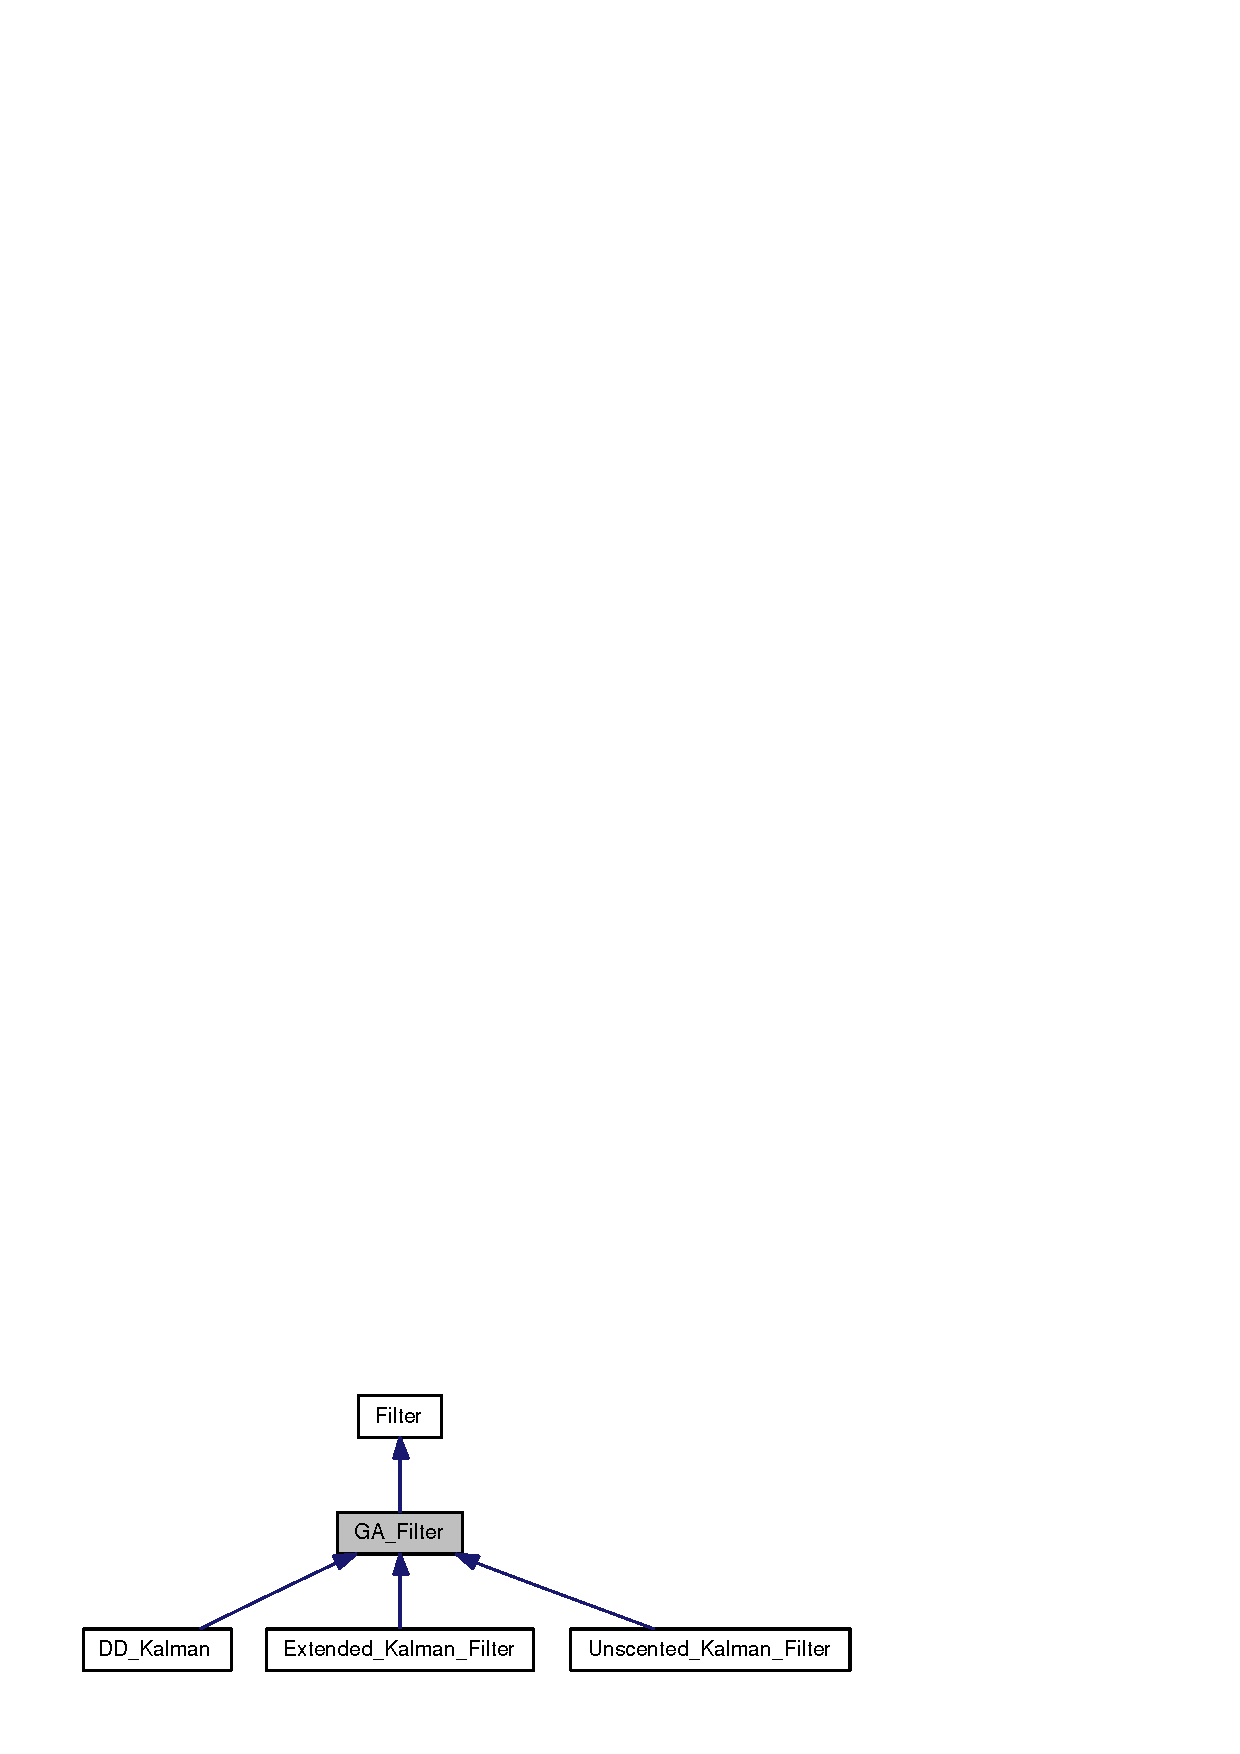
\includegraphics[width=400pt]{class_g_a___filter__inherit__graph}
\end{center}
\end{figure}
\subsection*{Public Member Functions}
\begin{CompactItemize}
\item 
\hyperlink{class_g_a___filter_7115851ae209079a5779026aa72aaaee}{GA\_\-Filter} (void)
\begin{CompactList}\small\item\em A constructor. \item\end{CompactList}\item 
\hyperlink{class_g_a___filter_07865b9b0bbc296fc1b156d4f0c9d4f4}{GA\_\-Filter} (\hyperlink{class_gaussian___nonlinear___model}{Gaussian\_\-Nonlinear\_\-Model} $\ast$m)
\item 
dcovector \hyperlink{class_g_a___filter_e92898cc15e34358cb9ecabd57067a39}{Expected\_\-Get} (void)
\end{CompactItemize}
\subsection*{Public Attributes}
\begin{CompactItemize}
\item 
dcovector \hyperlink{class_g_a___filter_8845e79b2c552edab83a18313bb48427}{M}
\begin{CompactList}\small\item\em The current mean $ \hat{X}_{k|k}=E[X_k |Y_{0:k}] $. \item\end{CompactList}\item 
dgematrix \hyperlink{class_g_a___filter_6a52a9cb2bbe7b568bdea626c951388f}{R}
\begin{CompactList}\small\item\em The current covariance $ \hat{P}_{k|k}=E[(X_k-\hat{X}_{k|k})(X_k-\hat{X}_{k|k})] $. \item\end{CompactList}\item 
dcovector \hyperlink{class_g_a___filter_9490630ecc3f4503003b8640eefe106a}{Xp}
\begin{CompactList}\small\item\em The prediction $ \hat{X}_{k-1|k}=E[X_{k-1} |Y_{0:k}] $. \item\end{CompactList}\item 
dgematrix \hyperlink{class_g_a___filter_7d6e23cf07e5b031d617f33ee25cab06}{Rp}
\begin{CompactList}\small\item\em The prediction covariance $ \hat{P}_{k-1|k}=E[(X_k-\hat{X}_{k-1|k})(X_k-\hat{X}_{k-1|k}) ] $. \item\end{CompactList}\end{CompactItemize}
\subsection*{Protected Member Functions}
\begin{CompactItemize}
\item 
virtual int \hyperlink{class_g_a___filter_7b5cb872bcedd752a4309f114625a4b8}{\_\-init} (void)
\end{CompactItemize}


\subsection{Detailed Description}
Abstract class of Gaussian Approximation filters. 

For discrete-discrete models (\hyperlink{class_gaussian___nonlinear___model}{Gaussian\_\-Nonlinear\_\-Model}), these filters approximate the probability density of the state transition $ p_{X_k|X_{k-1}} $ and the probability of the observation $ p_{Y_k|X_k} $ by gaussian densities. The approximation is exact in the case of linear model (\hyperlink{class_gaussian___linear___model}{Gaussian\_\-Linear\_\-Model}) and lead to the discrete-discrete Kalman \hyperlink{class_filter}{Filter} (\hyperlink{class_d_d___kalman}{DD\_\-Kalman}). For other non-linear models (\hyperlink{class_gaussian___nonlinear___model}{Gaussian\_\-Nonlinear\_\-Model}) UKF (\hyperlink{class_unscented___kalman___filter}{Unscented\_\-Kalman\_\-Filter}) or EKF (\hyperlink{class_extended___kalman___filter}{Extended\_\-Kalman\_\-Filter}) can be used. 

\subsection{Constructor \& Destructor Documentation}
\hypertarget{class_g_a___filter_7115851ae209079a5779026aa72aaaee}{
\index{GA\_\-Filter@{GA\_\-Filter}!GA\_\-Filter@{GA\_\-Filter}}
\index{GA\_\-Filter@{GA\_\-Filter}!GA_Filter@{GA\_\-Filter}}
\subsubsection[{GA\_\-Filter}]{\setlength{\rightskip}{0pt plus 5cm}GA\_\-Filter::GA\_\-Filter (void)}}
\label{class_g_a___filter_7115851ae209079a5779026aa72aaaee}


A constructor. 

\hypertarget{class_g_a___filter_07865b9b0bbc296fc1b156d4f0c9d4f4}{
\index{GA\_\-Filter@{GA\_\-Filter}!GA\_\-Filter@{GA\_\-Filter}}
\index{GA\_\-Filter@{GA\_\-Filter}!GA_Filter@{GA\_\-Filter}}
\subsubsection[{GA\_\-Filter}]{\setlength{\rightskip}{0pt plus 5cm}GA\_\-Filter::GA\_\-Filter ({\bf Gaussian\_\-Nonlinear\_\-Model} $\ast$ {\em m})}}
\label{class_g_a___filter_07865b9b0bbc296fc1b156d4f0c9d4f4}


A constructor

\begin{Desc}
\item[Parameters:]
\begin{description}
\item[{\em m}]A discrete-discrete gaussian non-linear model \end{description}
\end{Desc}


\subsection{Member Function Documentation}
\hypertarget{class_g_a___filter_7b5cb872bcedd752a4309f114625a4b8}{
\index{GA\_\-Filter@{GA\_\-Filter}!\_\-init@{\_\-init}}
\index{\_\-init@{\_\-init}!GA_Filter@{GA\_\-Filter}}
\subsubsection[{\_\-init}]{\setlength{\rightskip}{0pt plus 5cm}virtual int GA\_\-Filter::\_\-init (void)\hspace{0.3cm}{\tt  \mbox{[}protected, virtual\mbox{]}}}}
\label{class_g_a___filter_7b5cb872bcedd752a4309f114625a4b8}


Specific init for each filter

\begin{Desc}
\item[Parameters:]
\begin{description}
\item[{\em Y}]The observed sample\end{description}
\end{Desc}
\begin{Desc}
\item[Returns:]0 if no problem \end{Desc}


Implements \hyperlink{class_filter_f46a456184971270ca36733d937f14fb}{Filter}.

Reimplemented in \hyperlink{class_unscented___kalman___filter_a6ca6d9f8b5a4a40c18b6cdfdc2029fa}{Unscented\_\-Kalman\_\-Filter}.\hypertarget{class_g_a___filter_e92898cc15e34358cb9ecabd57067a39}{
\index{GA\_\-Filter@{GA\_\-Filter}!Expected\_\-Get@{Expected\_\-Get}}
\index{Expected\_\-Get@{Expected\_\-Get}!GA_Filter@{GA\_\-Filter}}
\subsubsection[{Expected\_\-Get}]{\setlength{\rightskip}{0pt plus 5cm}dcovector GA\_\-Filter::Expected\_\-Get (void)\hspace{0.3cm}{\tt  \mbox{[}virtual\mbox{]}}}}
\label{class_g_a___filter_e92898cc15e34358cb9ecabd57067a39}


Get the current estimation $ \hat{X}_{k|k} $

\begin{Desc}
\item[Returns:]$ \hat{X}_{k|k} $ \end{Desc}


Implements \hyperlink{class_filter_f6e41ec8ada47571291b31a259858cdc}{Filter}.

\subsection{Member Data Documentation}
\hypertarget{class_g_a___filter_8845e79b2c552edab83a18313bb48427}{
\index{GA\_\-Filter@{GA\_\-Filter}!M@{M}}
\index{M@{M}!GA_Filter@{GA\_\-Filter}}
\subsubsection[{M}]{\setlength{\rightskip}{0pt plus 5cm}dcovector {\bf GA\_\-Filter::M}}}
\label{class_g_a___filter_8845e79b2c552edab83a18313bb48427}


The current mean $ \hat{X}_{k|k}=E[X_k |Y_{0:k}] $. 

\hypertarget{class_g_a___filter_6a52a9cb2bbe7b568bdea626c951388f}{
\index{GA\_\-Filter@{GA\_\-Filter}!R@{R}}
\index{R@{R}!GA_Filter@{GA\_\-Filter}}
\subsubsection[{R}]{\setlength{\rightskip}{0pt plus 5cm}dgematrix {\bf GA\_\-Filter::R}}}
\label{class_g_a___filter_6a52a9cb2bbe7b568bdea626c951388f}


The current covariance $ \hat{P}_{k|k}=E[(X_k-\hat{X}_{k|k})(X_k-\hat{X}_{k|k})] $. 

\hypertarget{class_g_a___filter_7d6e23cf07e5b031d617f33ee25cab06}{
\index{GA\_\-Filter@{GA\_\-Filter}!Rp@{Rp}}
\index{Rp@{Rp}!GA_Filter@{GA\_\-Filter}}
\subsubsection[{Rp}]{\setlength{\rightskip}{0pt plus 5cm}dgematrix {\bf GA\_\-Filter::Rp}}}
\label{class_g_a___filter_7d6e23cf07e5b031d617f33ee25cab06}


The prediction covariance $ \hat{P}_{k-1|k}=E[(X_k-\hat{X}_{k-1|k})(X_k-\hat{X}_{k-1|k}) ] $. 

\hypertarget{class_g_a___filter_9490630ecc3f4503003b8640eefe106a}{
\index{GA\_\-Filter@{GA\_\-Filter}!Xp@{Xp}}
\index{Xp@{Xp}!GA_Filter@{GA\_\-Filter}}
\subsubsection[{Xp}]{\setlength{\rightskip}{0pt plus 5cm}dcovector {\bf GA\_\-Filter::Xp}}}
\label{class_g_a___filter_9490630ecc3f4503003b8640eefe106a}


The prediction $ \hat{X}_{k-1|k}=E[X_{k-1} |Y_{0:k}] $. 


\hypertarget{class_gaussian___linear___model}{
\section{Gaussian\_\-Linear\_\-Model Class Reference}
\label{class_gaussian___linear___model}\index{Gaussian\_\-Linear\_\-Model@{Gaussian\_\-Linear\_\-Model}}
}
Gaussian Linear \hyperlink{class_model}{Model} :.  


{\tt \#include $<$gaussian\_\-model.h$>$}

Inheritance diagram for Gaussian\_\-Linear\_\-Model:\nopagebreak
\begin{figure}[H]
\begin{center}
\leavevmode
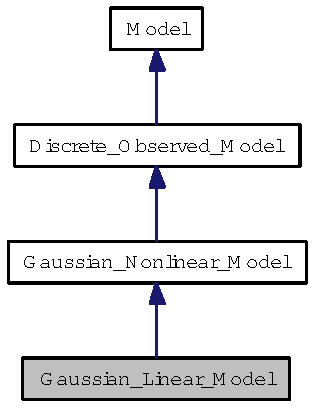
\includegraphics[width=93pt]{class_gaussian___linear___model__inherit__graph}
\end{center}
\end{figure}
\subsection*{Public Member Functions}
\begin{CompactItemize}
\item 
\hyperlink{class_gaussian___linear___model_495bfe0a795c2590a8476aff79613fa0}{Gaussian\_\-Linear\_\-Model} (void)
\item 
dcovector \hyperlink{class_gaussian___linear___model_f0d24016df8709697480126c240a16ba}{State\_\-Function} (const dcovector \&X, const dcovector \&W)
\begin{CompactList}\small\item\em The state Xk=F(Xk-1,Wk). \item\end{CompactList}\item 
dgematrix \hyperlink{class_gaussian___linear___model_3fb2cc6feae8997ad99fce7e2b77a2ce}{Jx\_\-State\_\-Function} (const dcovector \&X, const dcovector \&W)
\begin{CompactList}\small\item\em the X jacobian of the State function evaluate at X,W \item\end{CompactList}\item 
dgematrix \hyperlink{class_gaussian___linear___model_0df35cd7199676b9a03feec376aa49e7}{Jw\_\-State\_\-Function} (const dcovector \&X, const dcovector \&W)
\begin{CompactList}\small\item\em the W jacobian of the State function evaluate at X,W \item\end{CompactList}\item 
dcovector \hyperlink{class_gaussian___linear___model_85a8bede33982e2cd2e8433ae3f19ef5}{Get\_\-Mean\_\-Prediction} (const dcovector \&M)
\item 
dgematrix \hyperlink{class_gaussian___linear___model_93e0443c5a897a731f6f3b76d2fda62c}{Get\_\-Cov\_\-Prediction} (const dgematrix \&P)
\item 
dcovector \hyperlink{class_gaussian___linear___model_a6ac01291543509b33bad1160ad7e498}{Observation\_\-Function} (const dcovector \&X)
\begin{CompactList}\small\item\em The observation Yk=H(Xk) + Vk. \item\end{CompactList}\item 
dgematrix \hyperlink{class_gaussian___linear___model_ea76d88935c900fdc3e39775380446dc}{J\_\-Observation\_\-Function} (const dcovector \&X)
\begin{CompactList}\small\item\em the jacobian of the observation function evaluate at X \item\end{CompactList}\end{CompactItemize}
\subsection*{Public Attributes}
\begin{CompactItemize}
\item 
dgematrix \hyperlink{class_gaussian___linear___model_b0b82054668f84d9144f14023adbe43a}{F}
\item 
dgematrix \hyperlink{class_gaussian___linear___model_4d198f5e8f711cefb5de857b0cf28e6c}{G}
\item 
dcovector \hyperlink{class_gaussian___linear___model_397ff0f1b4258b548fe87b27af41fd64}{f}
\item 
dcovector \hyperlink{class_gaussian___linear___model_aa055db1eaa26e4c9387060a477be7a4}{h}
\item 
dgematrix \hyperlink{class_gaussian___linear___model_fe52ab90d715e5a58c7d64edfc846647}{H}
\end{CompactItemize}


\subsection{Detailed Description}
Gaussian Linear \hyperlink{class_model}{Model} :. 

The state : X(k) = F X(k-1) + f + G $\ast$ Wk The Observation Y(k) = H X(k) + h + V 

\subsection{Constructor \& Destructor Documentation}
\hypertarget{class_gaussian___linear___model_495bfe0a795c2590a8476aff79613fa0}{
\index{Gaussian\_\-Linear\_\-Model@{Gaussian\_\-Linear\_\-Model}!Gaussian\_\-Linear\_\-Model@{Gaussian\_\-Linear\_\-Model}}
\index{Gaussian\_\-Linear\_\-Model@{Gaussian\_\-Linear\_\-Model}!Gaussian_Linear_Model@{Gaussian\_\-Linear\_\-Model}}
\subsubsection[{Gaussian\_\-Linear\_\-Model}]{\setlength{\rightskip}{0pt plus 5cm}Gaussian\_\-Linear\_\-Model::Gaussian\_\-Linear\_\-Model (void)}}
\label{class_gaussian___linear___model_495bfe0a795c2590a8476aff79613fa0}




\subsection{Member Function Documentation}
\hypertarget{class_gaussian___linear___model_93e0443c5a897a731f6f3b76d2fda62c}{
\index{Gaussian\_\-Linear\_\-Model@{Gaussian\_\-Linear\_\-Model}!Get\_\-Cov\_\-Prediction@{Get\_\-Cov\_\-Prediction}}
\index{Get\_\-Cov\_\-Prediction@{Get\_\-Cov\_\-Prediction}!Gaussian_Linear_Model@{Gaussian\_\-Linear\_\-Model}}
\subsubsection[{Get\_\-Cov\_\-Prediction}]{\setlength{\rightskip}{0pt plus 5cm}dgematrix Gaussian\_\-Linear\_\-Model::Get\_\-Cov\_\-Prediction (const dgematrix \& {\em P})}}
\label{class_gaussian___linear___model_93e0443c5a897a731f6f3b76d2fda62c}


\hypertarget{class_gaussian___linear___model_85a8bede33982e2cd2e8433ae3f19ef5}{
\index{Gaussian\_\-Linear\_\-Model@{Gaussian\_\-Linear\_\-Model}!Get\_\-Mean\_\-Prediction@{Get\_\-Mean\_\-Prediction}}
\index{Get\_\-Mean\_\-Prediction@{Get\_\-Mean\_\-Prediction}!Gaussian_Linear_Model@{Gaussian\_\-Linear\_\-Model}}
\subsubsection[{Get\_\-Mean\_\-Prediction}]{\setlength{\rightskip}{0pt plus 5cm}dcovector Gaussian\_\-Linear\_\-Model::Get\_\-Mean\_\-Prediction (const dcovector \& {\em M})}}
\label{class_gaussian___linear___model_85a8bede33982e2cd2e8433ae3f19ef5}


\hypertarget{class_gaussian___linear___model_ea76d88935c900fdc3e39775380446dc}{
\index{Gaussian\_\-Linear\_\-Model@{Gaussian\_\-Linear\_\-Model}!J\_\-Observation\_\-Function@{J\_\-Observation\_\-Function}}
\index{J\_\-Observation\_\-Function@{J\_\-Observation\_\-Function}!Gaussian_Linear_Model@{Gaussian\_\-Linear\_\-Model}}
\subsubsection[{J\_\-Observation\_\-Function}]{\setlength{\rightskip}{0pt plus 5cm}dgematrix Gaussian\_\-Linear\_\-Model::J\_\-Observation\_\-Function (const dcovector \& {\em X})\hspace{0.3cm}{\tt  \mbox{[}virtual\mbox{]}}}}
\label{class_gaussian___linear___model_ea76d88935c900fdc3e39775380446dc}


the jacobian of the observation function evaluate at X 

\begin{Desc}
\item[Parameters:]
\begin{description}
\item[{\em X}]\end{description}
\end{Desc}
\begin{Desc}
\item[Returns:]The jacobian matrix \end{Desc}


Reimplemented from \hyperlink{class_discrete___observed___model_83cd1f2f54544d8977dbce844031f85e}{Discrete\_\-Observed\_\-Model}.\hypertarget{class_gaussian___linear___model_0df35cd7199676b9a03feec376aa49e7}{
\index{Gaussian\_\-Linear\_\-Model@{Gaussian\_\-Linear\_\-Model}!Jw\_\-State\_\-Function@{Jw\_\-State\_\-Function}}
\index{Jw\_\-State\_\-Function@{Jw\_\-State\_\-Function}!Gaussian_Linear_Model@{Gaussian\_\-Linear\_\-Model}}
\subsubsection[{Jw\_\-State\_\-Function}]{\setlength{\rightskip}{0pt plus 5cm}dgematrix Gaussian\_\-Linear\_\-Model::Jw\_\-State\_\-Function (const dcovector \& {\em X}, \/  const dcovector \& {\em W})\hspace{0.3cm}{\tt  \mbox{[}virtual\mbox{]}}}}
\label{class_gaussian___linear___model_0df35cd7199676b9a03feec376aa49e7}


the W jacobian of the State function evaluate at X,W 

\begin{Desc}
\item[Parameters:]
\begin{description}
\item[{\em X}]evaluate at X \item[{\em W}]evalate at W\end{description}
\end{Desc}
\begin{Desc}
\item[Returns:]The jacobian matrix \end{Desc}


Reimplemented from \hyperlink{class_gaussian___nonlinear___model_1c6710cedf6317e07b7b2a48f41f5442}{Gaussian\_\-Nonlinear\_\-Model}.\hypertarget{class_gaussian___linear___model_3fb2cc6feae8997ad99fce7e2b77a2ce}{
\index{Gaussian\_\-Linear\_\-Model@{Gaussian\_\-Linear\_\-Model}!Jx\_\-State\_\-Function@{Jx\_\-State\_\-Function}}
\index{Jx\_\-State\_\-Function@{Jx\_\-State\_\-Function}!Gaussian_Linear_Model@{Gaussian\_\-Linear\_\-Model}}
\subsubsection[{Jx\_\-State\_\-Function}]{\setlength{\rightskip}{0pt plus 5cm}dgematrix Gaussian\_\-Linear\_\-Model::Jx\_\-State\_\-Function (const dcovector \& {\em X}, \/  const dcovector \& {\em W})\hspace{0.3cm}{\tt  \mbox{[}virtual\mbox{]}}}}
\label{class_gaussian___linear___model_3fb2cc6feae8997ad99fce7e2b77a2ce}


the X jacobian of the State function evaluate at X,W 

\begin{Desc}
\item[Parameters:]
\begin{description}
\item[{\em X}]evaluate at X \item[{\em W}]evalate at W\end{description}
\end{Desc}
\begin{Desc}
\item[Returns:]The jacobian matrix \end{Desc}


Reimplemented from \hyperlink{class_gaussian___nonlinear___model_ad4a587fcaab06d2d9e44d61cee814cf}{Gaussian\_\-Nonlinear\_\-Model}.\hypertarget{class_gaussian___linear___model_a6ac01291543509b33bad1160ad7e498}{
\index{Gaussian\_\-Linear\_\-Model@{Gaussian\_\-Linear\_\-Model}!Observation\_\-Function@{Observation\_\-Function}}
\index{Observation\_\-Function@{Observation\_\-Function}!Gaussian_Linear_Model@{Gaussian\_\-Linear\_\-Model}}
\subsubsection[{Observation\_\-Function}]{\setlength{\rightskip}{0pt plus 5cm}dcovector Gaussian\_\-Linear\_\-Model::Observation\_\-Function (const dcovector \& {\em X})\hspace{0.3cm}{\tt  \mbox{[}virtual\mbox{]}}}}
\label{class_gaussian___linear___model_a6ac01291543509b33bad1160ad7e498}


The observation Yk=H(Xk) + Vk. 

\begin{Desc}
\item[Parameters:]
\begin{description}
\item[{\em X}]The state at k\end{description}
\end{Desc}
\begin{Desc}
\item[Returns:]The observation at k \end{Desc}


Implements \hyperlink{class_discrete___observed___model_8d56d86ea6b204672c8ebd720f1e11a6}{Discrete\_\-Observed\_\-Model}.\hypertarget{class_gaussian___linear___model_f0d24016df8709697480126c240a16ba}{
\index{Gaussian\_\-Linear\_\-Model@{Gaussian\_\-Linear\_\-Model}!State\_\-Function@{State\_\-Function}}
\index{State\_\-Function@{State\_\-Function}!Gaussian_Linear_Model@{Gaussian\_\-Linear\_\-Model}}
\subsubsection[{State\_\-Function}]{\setlength{\rightskip}{0pt plus 5cm}dcovector Gaussian\_\-Linear\_\-Model::State\_\-Function (const dcovector \& {\em X}, \/  const dcovector \& {\em W})\hspace{0.3cm}{\tt  \mbox{[}virtual\mbox{]}}}}
\label{class_gaussian___linear___model_f0d24016df8709697480126c240a16ba}


The state Xk=F(Xk-1,Wk). 

\begin{Desc}
\item[Parameters:]
\begin{description}
\item[{\em X}]The state at k-1 \item[{\em W}]The Noise\end{description}
\end{Desc}
\begin{Desc}
\item[Returns:]The state at k \end{Desc}


Implements \hyperlink{class_gaussian___nonlinear___model_df0e6cf50a8d5fdb6decd05046867cd8}{Gaussian\_\-Nonlinear\_\-Model}.

\subsection{Member Data Documentation}
\hypertarget{class_gaussian___linear___model_397ff0f1b4258b548fe87b27af41fd64}{
\index{Gaussian\_\-Linear\_\-Model@{Gaussian\_\-Linear\_\-Model}!f@{f}}
\index{f@{f}!Gaussian_Linear_Model@{Gaussian\_\-Linear\_\-Model}}
\subsubsection[{f}]{\setlength{\rightskip}{0pt plus 5cm}dcovector {\bf Gaussian\_\-Linear\_\-Model::f}}}
\label{class_gaussian___linear___model_397ff0f1b4258b548fe87b27af41fd64}


\hypertarget{class_gaussian___linear___model_b0b82054668f84d9144f14023adbe43a}{
\index{Gaussian\_\-Linear\_\-Model@{Gaussian\_\-Linear\_\-Model}!F@{F}}
\index{F@{F}!Gaussian_Linear_Model@{Gaussian\_\-Linear\_\-Model}}
\subsubsection[{F}]{\setlength{\rightskip}{0pt plus 5cm}dgematrix {\bf Gaussian\_\-Linear\_\-Model::F}}}
\label{class_gaussian___linear___model_b0b82054668f84d9144f14023adbe43a}


\hypertarget{class_gaussian___linear___model_4d198f5e8f711cefb5de857b0cf28e6c}{
\index{Gaussian\_\-Linear\_\-Model@{Gaussian\_\-Linear\_\-Model}!G@{G}}
\index{G@{G}!Gaussian_Linear_Model@{Gaussian\_\-Linear\_\-Model}}
\subsubsection[{G}]{\setlength{\rightskip}{0pt plus 5cm}dgematrix {\bf Gaussian\_\-Linear\_\-Model::G}}}
\label{class_gaussian___linear___model_4d198f5e8f711cefb5de857b0cf28e6c}


\hypertarget{class_gaussian___linear___model_fe52ab90d715e5a58c7d64edfc846647}{
\index{Gaussian\_\-Linear\_\-Model@{Gaussian\_\-Linear\_\-Model}!H@{H}}
\index{H@{H}!Gaussian_Linear_Model@{Gaussian\_\-Linear\_\-Model}}
\subsubsection[{H}]{\setlength{\rightskip}{0pt plus 5cm}dgematrix {\bf Gaussian\_\-Linear\_\-Model::H}}}
\label{class_gaussian___linear___model_fe52ab90d715e5a58c7d64edfc846647}


\hypertarget{class_gaussian___linear___model_aa055db1eaa26e4c9387060a477be7a4}{
\index{Gaussian\_\-Linear\_\-Model@{Gaussian\_\-Linear\_\-Model}!h@{h}}
\index{h@{h}!Gaussian_Linear_Model@{Gaussian\_\-Linear\_\-Model}}
\subsubsection[{h}]{\setlength{\rightskip}{0pt plus 5cm}dcovector {\bf Gaussian\_\-Linear\_\-Model::h}}}
\label{class_gaussian___linear___model_aa055db1eaa26e4c9387060a477be7a4}



\hypertarget{class_gaussian___nonlinear___model}{
\section{Gaussian\_\-Nonlinear\_\-Model Class Reference}
\label{class_gaussian___nonlinear___model}\index{Gaussian\_\-Nonlinear\_\-Model@{Gaussian\_\-Nonlinear\_\-Model}}
}
Gaussian Nonlinear \hyperlink{class_model}{Model} The state : X(k) = F (Xk-1, Wk) The Observation Y(k) = H (X(k)) + V.  


{\tt \#include $<$gaussian\_\-model.h$>$}

Inheritance diagram for Gaussian\_\-Nonlinear\_\-Model:\nopagebreak
\begin{figure}[H]
\begin{center}
\leavevmode
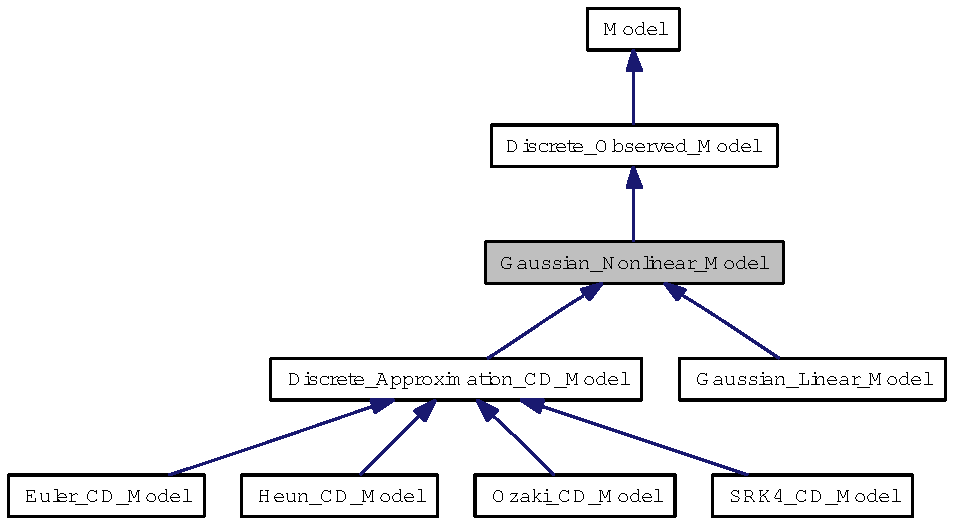
\includegraphics[width=400pt]{class_gaussian___nonlinear___model__inherit__graph}
\end{center}
\end{figure}
\subsection*{Public Member Functions}
\begin{CompactItemize}
\item 
\hyperlink{class_gaussian___nonlinear___model_59d94561c9b95d4b510f244a198c29a0}{Gaussian\_\-Nonlinear\_\-Model} (void)
\item 
virtual \hyperlink{class_gaussian___nonlinear___model_35fe0f1156e0d0e687937df527aea1e0}{$\sim$Gaussian\_\-Nonlinear\_\-Model} (void)
\item 
virtual void \hyperlink{class_gaussian___nonlinear___model_146f819d0aeea0dc59b86e9af200e0bd}{Init} (void)
\begin{CompactList}\small\item\em Init The model if needed. \item\end{CompactList}\item 
virtual dcovector \hyperlink{class_gaussian___nonlinear___model_df0e6cf50a8d5fdb6decd05046867cd8}{State\_\-Function} (const dcovector \&X, const dcovector \&W)=0
\begin{CompactList}\small\item\em The state Xk=F(Xk-1,Wk). \item\end{CompactList}\item 
virtual dgematrix \hyperlink{class_gaussian___nonlinear___model_ad4a587fcaab06d2d9e44d61cee814cf}{Jx\_\-State\_\-Function} (const dcovector \&X, const dcovector \&W)
\begin{CompactList}\small\item\em the X jacobian of the State function evaluate at X,W \item\end{CompactList}\item 
virtual dgematrix \hyperlink{class_gaussian___nonlinear___model_1c6710cedf6317e07b7b2a48f41f5442}{Jw\_\-State\_\-Function} (const dcovector \&X, const dcovector \&W)
\begin{CompactList}\small\item\em the W jacobian of the State function evaluate at X,W \item\end{CompactList}\item 
virtual void \hyperlink{class_gaussian___nonlinear___model_c850a678b4672e4358d3f29d7b998549}{Get\_\-Linear\_\-Parameters} (const dcovector \&X, const dcovector \&W, dgematrix \&F, dgematrix \&G, dcovector \&Xp)
\begin{CompactList}\small\item\em computed linearized parameter for EKF in X,W \item\end{CompactList}\end{CompactItemize}


\subsection{Detailed Description}
Gaussian Nonlinear \hyperlink{class_model}{Model} The state : X(k) = F (Xk-1, Wk) The Observation Y(k) = H (X(k)) + V. 

\subsection{Constructor \& Destructor Documentation}
\hypertarget{class_gaussian___nonlinear___model_59d94561c9b95d4b510f244a198c29a0}{
\index{Gaussian\_\-Nonlinear\_\-Model@{Gaussian\_\-Nonlinear\_\-Model}!Gaussian\_\-Nonlinear\_\-Model@{Gaussian\_\-Nonlinear\_\-Model}}
\index{Gaussian\_\-Nonlinear\_\-Model@{Gaussian\_\-Nonlinear\_\-Model}!Gaussian_Nonlinear_Model@{Gaussian\_\-Nonlinear\_\-Model}}
\subsubsection[{Gaussian\_\-Nonlinear\_\-Model}]{\setlength{\rightskip}{0pt plus 5cm}Gaussian\_\-Nonlinear\_\-Model::Gaussian\_\-Nonlinear\_\-Model (void)}}
\label{class_gaussian___nonlinear___model_59d94561c9b95d4b510f244a198c29a0}


\hypertarget{class_gaussian___nonlinear___model_35fe0f1156e0d0e687937df527aea1e0}{
\index{Gaussian\_\-Nonlinear\_\-Model@{Gaussian\_\-Nonlinear\_\-Model}!$\sim$Gaussian\_\-Nonlinear\_\-Model@{$\sim$Gaussian\_\-Nonlinear\_\-Model}}
\index{$\sim$Gaussian\_\-Nonlinear\_\-Model@{$\sim$Gaussian\_\-Nonlinear\_\-Model}!Gaussian_Nonlinear_Model@{Gaussian\_\-Nonlinear\_\-Model}}
\subsubsection[{$\sim$Gaussian\_\-Nonlinear\_\-Model}]{\setlength{\rightskip}{0pt plus 5cm}virtual Gaussian\_\-Nonlinear\_\-Model::$\sim$Gaussian\_\-Nonlinear\_\-Model (void)\hspace{0.3cm}{\tt  \mbox{[}virtual\mbox{]}}}}
\label{class_gaussian___nonlinear___model_35fe0f1156e0d0e687937df527aea1e0}




\subsection{Member Function Documentation}
\hypertarget{class_gaussian___nonlinear___model_c850a678b4672e4358d3f29d7b998549}{
\index{Gaussian\_\-Nonlinear\_\-Model@{Gaussian\_\-Nonlinear\_\-Model}!Get\_\-Linear\_\-Parameters@{Get\_\-Linear\_\-Parameters}}
\index{Get\_\-Linear\_\-Parameters@{Get\_\-Linear\_\-Parameters}!Gaussian_Nonlinear_Model@{Gaussian\_\-Nonlinear\_\-Model}}
\subsubsection[{Get\_\-Linear\_\-Parameters}]{\setlength{\rightskip}{0pt plus 5cm}virtual void Gaussian\_\-Nonlinear\_\-Model::Get\_\-Linear\_\-Parameters (const dcovector \& {\em X}, \/  const dcovector \& {\em W}, \/  dgematrix \& {\em F}, \/  dgematrix \& {\em G}, \/  dcovector \& {\em Xp})\hspace{0.3cm}{\tt  \mbox{[}virtual\mbox{]}}}}
\label{class_gaussian___nonlinear___model_c850a678b4672e4358d3f29d7b998549}


computed linearized parameter for EKF in X,W 

\begin{Desc}
\item[Parameters:]
\begin{description}
\item[{\em X}]The state value \item[{\em W}]The noise value \item[{\em F}]The jacobian of f(X,W) in X \item[{\em G}]The jacobian in f(X,W) in W \item[{\em Xp}]The prediction Xp = f(X,W) \end{description}
\end{Desc}


Reimplemented in \hyperlink{class_discrete___approximation___c_d___model_445e1215275e1f77f6260a186e9f842a}{Discrete\_\-Approximation\_\-CD\_\-Model}.\hypertarget{class_gaussian___nonlinear___model_146f819d0aeea0dc59b86e9af200e0bd}{
\index{Gaussian\_\-Nonlinear\_\-Model@{Gaussian\_\-Nonlinear\_\-Model}!Init@{Init}}
\index{Init@{Init}!Gaussian_Nonlinear_Model@{Gaussian\_\-Nonlinear\_\-Model}}
\subsubsection[{Init}]{\setlength{\rightskip}{0pt plus 5cm}virtual void Gaussian\_\-Nonlinear\_\-Model::Init (void)\hspace{0.3cm}{\tt  \mbox{[}virtual\mbox{]}}}}
\label{class_gaussian___nonlinear___model_146f819d0aeea0dc59b86e9af200e0bd}


Init The model if needed. 



Reimplemented in \hyperlink{class_discrete___approximation___c_d___model_0c4caaf9a2874a8e5219e72401caf908}{Discrete\_\-Approximation\_\-CD\_\-Model}.\hypertarget{class_gaussian___nonlinear___model_1c6710cedf6317e07b7b2a48f41f5442}{
\index{Gaussian\_\-Nonlinear\_\-Model@{Gaussian\_\-Nonlinear\_\-Model}!Jw\_\-State\_\-Function@{Jw\_\-State\_\-Function}}
\index{Jw\_\-State\_\-Function@{Jw\_\-State\_\-Function}!Gaussian_Nonlinear_Model@{Gaussian\_\-Nonlinear\_\-Model}}
\subsubsection[{Jw\_\-State\_\-Function}]{\setlength{\rightskip}{0pt plus 5cm}virtual dgematrix Gaussian\_\-Nonlinear\_\-Model::Jw\_\-State\_\-Function (const dcovector \& {\em X}, \/  const dcovector \& {\em W})\hspace{0.3cm}{\tt  \mbox{[}virtual\mbox{]}}}}
\label{class_gaussian___nonlinear___model_1c6710cedf6317e07b7b2a48f41f5442}


the W jacobian of the State function evaluate at X,W 

\begin{Desc}
\item[Parameters:]
\begin{description}
\item[{\em X}]evaluate at X \item[{\em W}]evalate at W\end{description}
\end{Desc}
\begin{Desc}
\item[Returns:]The jacobian matrix \end{Desc}


Reimplemented in \hyperlink{class_gaussian___linear___model_0df35cd7199676b9a03feec376aa49e7}{Gaussian\_\-Linear\_\-Model}, and \hyperlink{class_discrete___approximation___c_d___model_a5021c3ba6bd2cce5558a783843461ab}{Discrete\_\-Approximation\_\-CD\_\-Model}.\hypertarget{class_gaussian___nonlinear___model_ad4a587fcaab06d2d9e44d61cee814cf}{
\index{Gaussian\_\-Nonlinear\_\-Model@{Gaussian\_\-Nonlinear\_\-Model}!Jx\_\-State\_\-Function@{Jx\_\-State\_\-Function}}
\index{Jx\_\-State\_\-Function@{Jx\_\-State\_\-Function}!Gaussian_Nonlinear_Model@{Gaussian\_\-Nonlinear\_\-Model}}
\subsubsection[{Jx\_\-State\_\-Function}]{\setlength{\rightskip}{0pt plus 5cm}virtual dgematrix Gaussian\_\-Nonlinear\_\-Model::Jx\_\-State\_\-Function (const dcovector \& {\em X}, \/  const dcovector \& {\em W})\hspace{0.3cm}{\tt  \mbox{[}virtual\mbox{]}}}}
\label{class_gaussian___nonlinear___model_ad4a587fcaab06d2d9e44d61cee814cf}


the X jacobian of the State function evaluate at X,W 

\begin{Desc}
\item[Parameters:]
\begin{description}
\item[{\em X}]evaluate at X \item[{\em W}]evalate at W\end{description}
\end{Desc}
\begin{Desc}
\item[Returns:]The jacobian matrix \end{Desc}


Reimplemented in \hyperlink{class_gaussian___linear___model_3fb2cc6feae8997ad99fce7e2b77a2ce}{Gaussian\_\-Linear\_\-Model}, and \hyperlink{class_discrete___approximation___c_d___model_b0ba3cda373913f6a1df4a417200218a}{Discrete\_\-Approximation\_\-CD\_\-Model}.\hypertarget{class_gaussian___nonlinear___model_df0e6cf50a8d5fdb6decd05046867cd8}{
\index{Gaussian\_\-Nonlinear\_\-Model@{Gaussian\_\-Nonlinear\_\-Model}!State\_\-Function@{State\_\-Function}}
\index{State\_\-Function@{State\_\-Function}!Gaussian_Nonlinear_Model@{Gaussian\_\-Nonlinear\_\-Model}}
\subsubsection[{State\_\-Function}]{\setlength{\rightskip}{0pt plus 5cm}virtual dcovector Gaussian\_\-Nonlinear\_\-Model::State\_\-Function (const dcovector \& {\em X}, \/  const dcovector \& {\em W})\hspace{0.3cm}{\tt  \mbox{[}pure virtual\mbox{]}}}}
\label{class_gaussian___nonlinear___model_df0e6cf50a8d5fdb6decd05046867cd8}


The state Xk=F(Xk-1,Wk). 

\begin{Desc}
\item[Parameters:]
\begin{description}
\item[{\em X}]The state at k-1 \item[{\em W}]The Noise\end{description}
\end{Desc}
\begin{Desc}
\item[Returns:]The state at k \end{Desc}


Implemented in \hyperlink{class_gaussian___linear___model_f0d24016df8709697480126c240a16ba}{Gaussian\_\-Linear\_\-Model}, and \hyperlink{class_discrete___approximation___c_d___model_83ef21b9993bfbef655874ca38777131}{Discrete\_\-Approximation\_\-CD\_\-Model}.
\hypertarget{class_heun___c_d___model}{
\section{Heun\_\-CD\_\-Model Class Reference}
\label{class_heun___c_d___model}\index{Heun\_\-CD\_\-Model@{Heun\_\-CD\_\-Model}}
}
continuous discret model: the state SDE is discretly approximate by an Sstochastic Heun method  


{\tt \#include $<$gaussian\_\-model.h$>$}

Inheritance diagram for Heun\_\-CD\_\-Model:\nopagebreak
\begin{figure}[H]
\begin{center}
\leavevmode
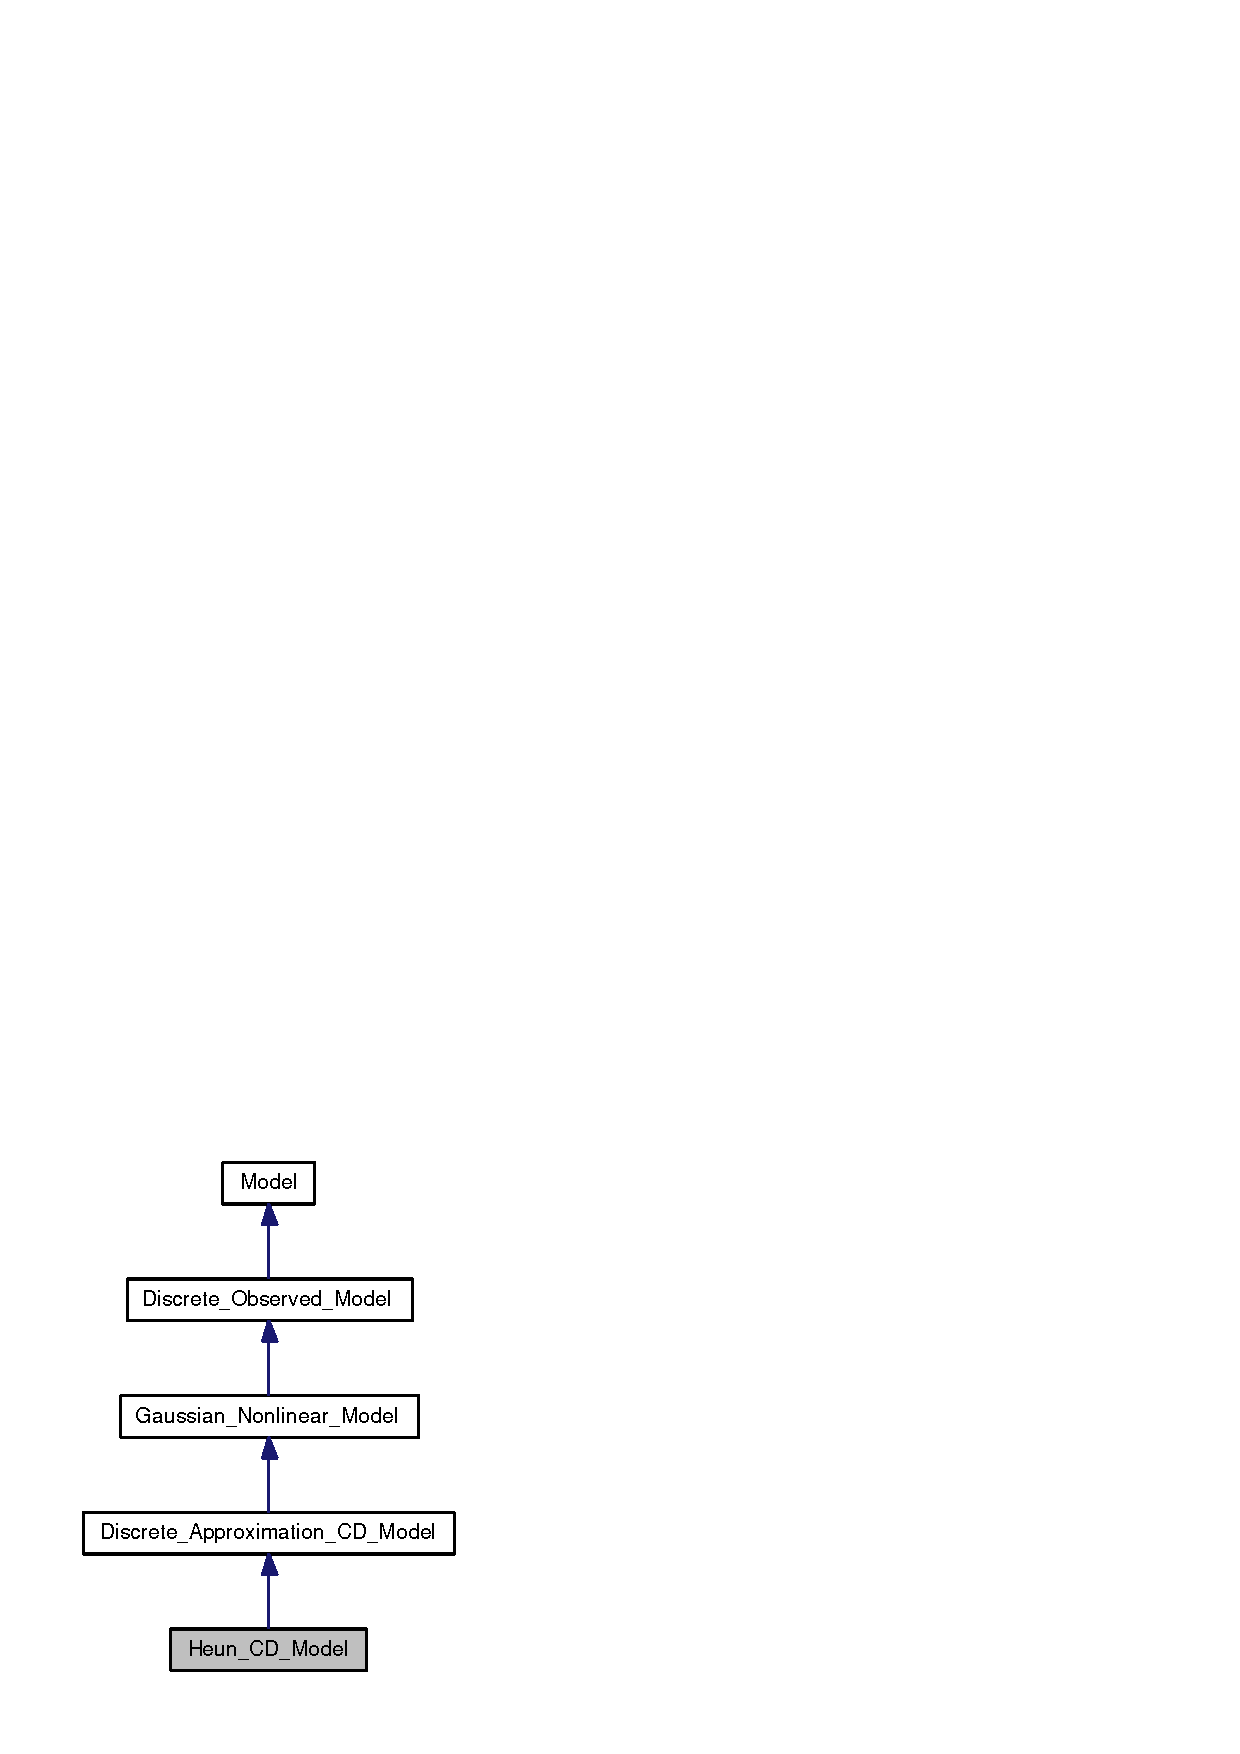
\includegraphics[width=111pt]{class_heun___c_d___model__inherit__graph}
\end{center}
\end{figure}
\subsection*{Public Member Functions}
\begin{CompactItemize}
\item 
\hyperlink{class_heun___c_d___model_1fa492e132304f4dbd1c722c1cd0d9a5}{Heun\_\-CD\_\-Model} (void)
\item 
\hyperlink{class_heun___c_d___model_4a6a03c0d4fd6381c0ba150761cec1cc}{Heun\_\-CD\_\-Model} (\hyperlink{class_continuous___discrete___model}{Continuous\_\-Discrete\_\-Model} $\ast$m, const int \&a)
\item 
dcovector \hyperlink{class_heun___c_d___model_98a85a23296e6c9f422f12063ece307b}{Scheme} (const dcovector \&X, const dcovector \&W)
\item 
dgematrix \hyperlink{class_heun___c_d___model_322cd83c0b81c2ed81483f42123f08e6}{Jx\_\-Scheme} (const dcovector \&X, const dcovector \&W)
\item 
dgematrix \hyperlink{class_heun___c_d___model_000fb9b8dbfb8171b8f330d7fc6d0dce}{Jw\_\-Scheme} (const dcovector \&X, const dcovector \&W)
\item 
void \hyperlink{class_heun___c_d___model_38c51141d41b3c92509ab2c6040fd2cd}{Get\_\-Linear\_\-Scheme} (const dcovector \&X, const dcovector \&W, dgematrix \&F, dgematrix \&J, dcovector \&Xp)
\begin{CompactList}\small\item\em Get the Linearized parameters Scheme in X,W. \item\end{CompactList}\end{CompactItemize}


\subsection{Detailed Description}
continuous discret model: the state SDE is discretly approximate by an Sstochastic Heun method 

\subsection{Constructor \& Destructor Documentation}
\hypertarget{class_heun___c_d___model_1fa492e132304f4dbd1c722c1cd0d9a5}{
\index{Heun\_\-CD\_\-Model@{Heun\_\-CD\_\-Model}!Heun\_\-CD\_\-Model@{Heun\_\-CD\_\-Model}}
\index{Heun\_\-CD\_\-Model@{Heun\_\-CD\_\-Model}!Heun_CD_Model@{Heun\_\-CD\_\-Model}}
\subsubsection[{Heun\_\-CD\_\-Model}]{\setlength{\rightskip}{0pt plus 5cm}Heun\_\-CD\_\-Model::Heun\_\-CD\_\-Model (void)}}
\label{class_heun___c_d___model_1fa492e132304f4dbd1c722c1cd0d9a5}


\hypertarget{class_heun___c_d___model_4a6a03c0d4fd6381c0ba150761cec1cc}{
\index{Heun\_\-CD\_\-Model@{Heun\_\-CD\_\-Model}!Heun\_\-CD\_\-Model@{Heun\_\-CD\_\-Model}}
\index{Heun\_\-CD\_\-Model@{Heun\_\-CD\_\-Model}!Heun_CD_Model@{Heun\_\-CD\_\-Model}}
\subsubsection[{Heun\_\-CD\_\-Model}]{\setlength{\rightskip}{0pt plus 5cm}Heun\_\-CD\_\-Model::Heun\_\-CD\_\-Model ({\bf Continuous\_\-Discrete\_\-Model} $\ast$ {\em m}, \/  const int \& {\em a})}}
\label{class_heun___c_d___model_4a6a03c0d4fd6381c0ba150761cec1cc}




\subsection{Member Function Documentation}
\hypertarget{class_heun___c_d___model_38c51141d41b3c92509ab2c6040fd2cd}{
\index{Heun\_\-CD\_\-Model@{Heun\_\-CD\_\-Model}!Get\_\-Linear\_\-Scheme@{Get\_\-Linear\_\-Scheme}}
\index{Get\_\-Linear\_\-Scheme@{Get\_\-Linear\_\-Scheme}!Heun_CD_Model@{Heun\_\-CD\_\-Model}}
\subsubsection[{Get\_\-Linear\_\-Scheme}]{\setlength{\rightskip}{0pt plus 5cm}void Heun\_\-CD\_\-Model::Get\_\-Linear\_\-Scheme (const dcovector \& {\em X}, \/  const dcovector \& {\em W}, \/  dgematrix \& {\em F}, \/  dgematrix \& {\em J}, \/  dcovector \& {\em Xp})\hspace{0.3cm}{\tt  \mbox{[}virtual\mbox{]}}}}
\label{class_heun___c_d___model_38c51141d41b3c92509ab2c6040fd2cd}


Get the Linearized parameters Scheme in X,W. 

\begin{Desc}
\item[Parameters:]
\begin{description}
\item[{\em X}]The state value \item[{\em W}]The noise value \item[{\em F}]The jacobian of f(X,W) in X \item[{\em G}]The jacobian in f(X,W) in W \item[{\em Xp}]The prediction Xp = f(X,W) \end{description}
\end{Desc}


Implements \hyperlink{class_discrete___approximation___c_d___model_0a486fada10e6f5569d186edc7b32110}{Discrete\_\-Approximation\_\-CD\_\-Model}.\hypertarget{class_heun___c_d___model_000fb9b8dbfb8171b8f330d7fc6d0dce}{
\index{Heun\_\-CD\_\-Model@{Heun\_\-CD\_\-Model}!Jw\_\-Scheme@{Jw\_\-Scheme}}
\index{Jw\_\-Scheme@{Jw\_\-Scheme}!Heun_CD_Model@{Heun\_\-CD\_\-Model}}
\subsubsection[{Jw\_\-Scheme}]{\setlength{\rightskip}{0pt plus 5cm}dgematrix Heun\_\-CD\_\-Model::Jw\_\-Scheme (const dcovector \& {\em X}, \/  const dcovector \& {\em W})\hspace{0.3cm}{\tt  \mbox{[}virtual\mbox{]}}}}
\label{class_heun___c_d___model_000fb9b8dbfb8171b8f330d7fc6d0dce}




Implements \hyperlink{class_discrete___approximation___c_d___model_c7496999409a3f05125ceb7fe85e85ab}{Discrete\_\-Approximation\_\-CD\_\-Model}.\hypertarget{class_heun___c_d___model_322cd83c0b81c2ed81483f42123f08e6}{
\index{Heun\_\-CD\_\-Model@{Heun\_\-CD\_\-Model}!Jx\_\-Scheme@{Jx\_\-Scheme}}
\index{Jx\_\-Scheme@{Jx\_\-Scheme}!Heun_CD_Model@{Heun\_\-CD\_\-Model}}
\subsubsection[{Jx\_\-Scheme}]{\setlength{\rightskip}{0pt plus 5cm}dgematrix Heun\_\-CD\_\-Model::Jx\_\-Scheme (const dcovector \& {\em X}, \/  const dcovector \& {\em W})\hspace{0.3cm}{\tt  \mbox{[}virtual\mbox{]}}}}
\label{class_heun___c_d___model_322cd83c0b81c2ed81483f42123f08e6}




Implements \hyperlink{class_discrete___approximation___c_d___model_7a3dcae055d90be0b8a231eff961e2a2}{Discrete\_\-Approximation\_\-CD\_\-Model}.\hypertarget{class_heun___c_d___model_98a85a23296e6c9f422f12063ece307b}{
\index{Heun\_\-CD\_\-Model@{Heun\_\-CD\_\-Model}!Scheme@{Scheme}}
\index{Scheme@{Scheme}!Heun_CD_Model@{Heun\_\-CD\_\-Model}}
\subsubsection[{Scheme}]{\setlength{\rightskip}{0pt plus 5cm}dcovector Heun\_\-CD\_\-Model::Scheme (const dcovector \& {\em X}, \/  const dcovector \& {\em W})\hspace{0.3cm}{\tt  \mbox{[}virtual\mbox{]}}}}
\label{class_heun___c_d___model_98a85a23296e6c9f422f12063ece307b}




Implements \hyperlink{class_discrete___approximation___c_d___model_1ea9a1d618890fc51db6fa98eeb7af7f}{Discrete\_\-Approximation\_\-CD\_\-Model}.
\hypertarget{class_linear___c_d___model}{
\section{Linear\_\-CD\_\-Model Class Reference}
\label{class_linear___c_d___model}\index{Linear\_\-CD\_\-Model@{Linear\_\-CD\_\-Model}}
}
Linear continuous discrete model class of the form dx = AX dt + Bdt + CdW Y\_\-k = HX(t\_\-k) + h + V\_\-k.  


{\tt \#include $<$gaussian\_\-model.h$>$}

Inheritance diagram for Linear\_\-CD\_\-Model:\nopagebreak
\begin{figure}[H]
\begin{center}
\leavevmode
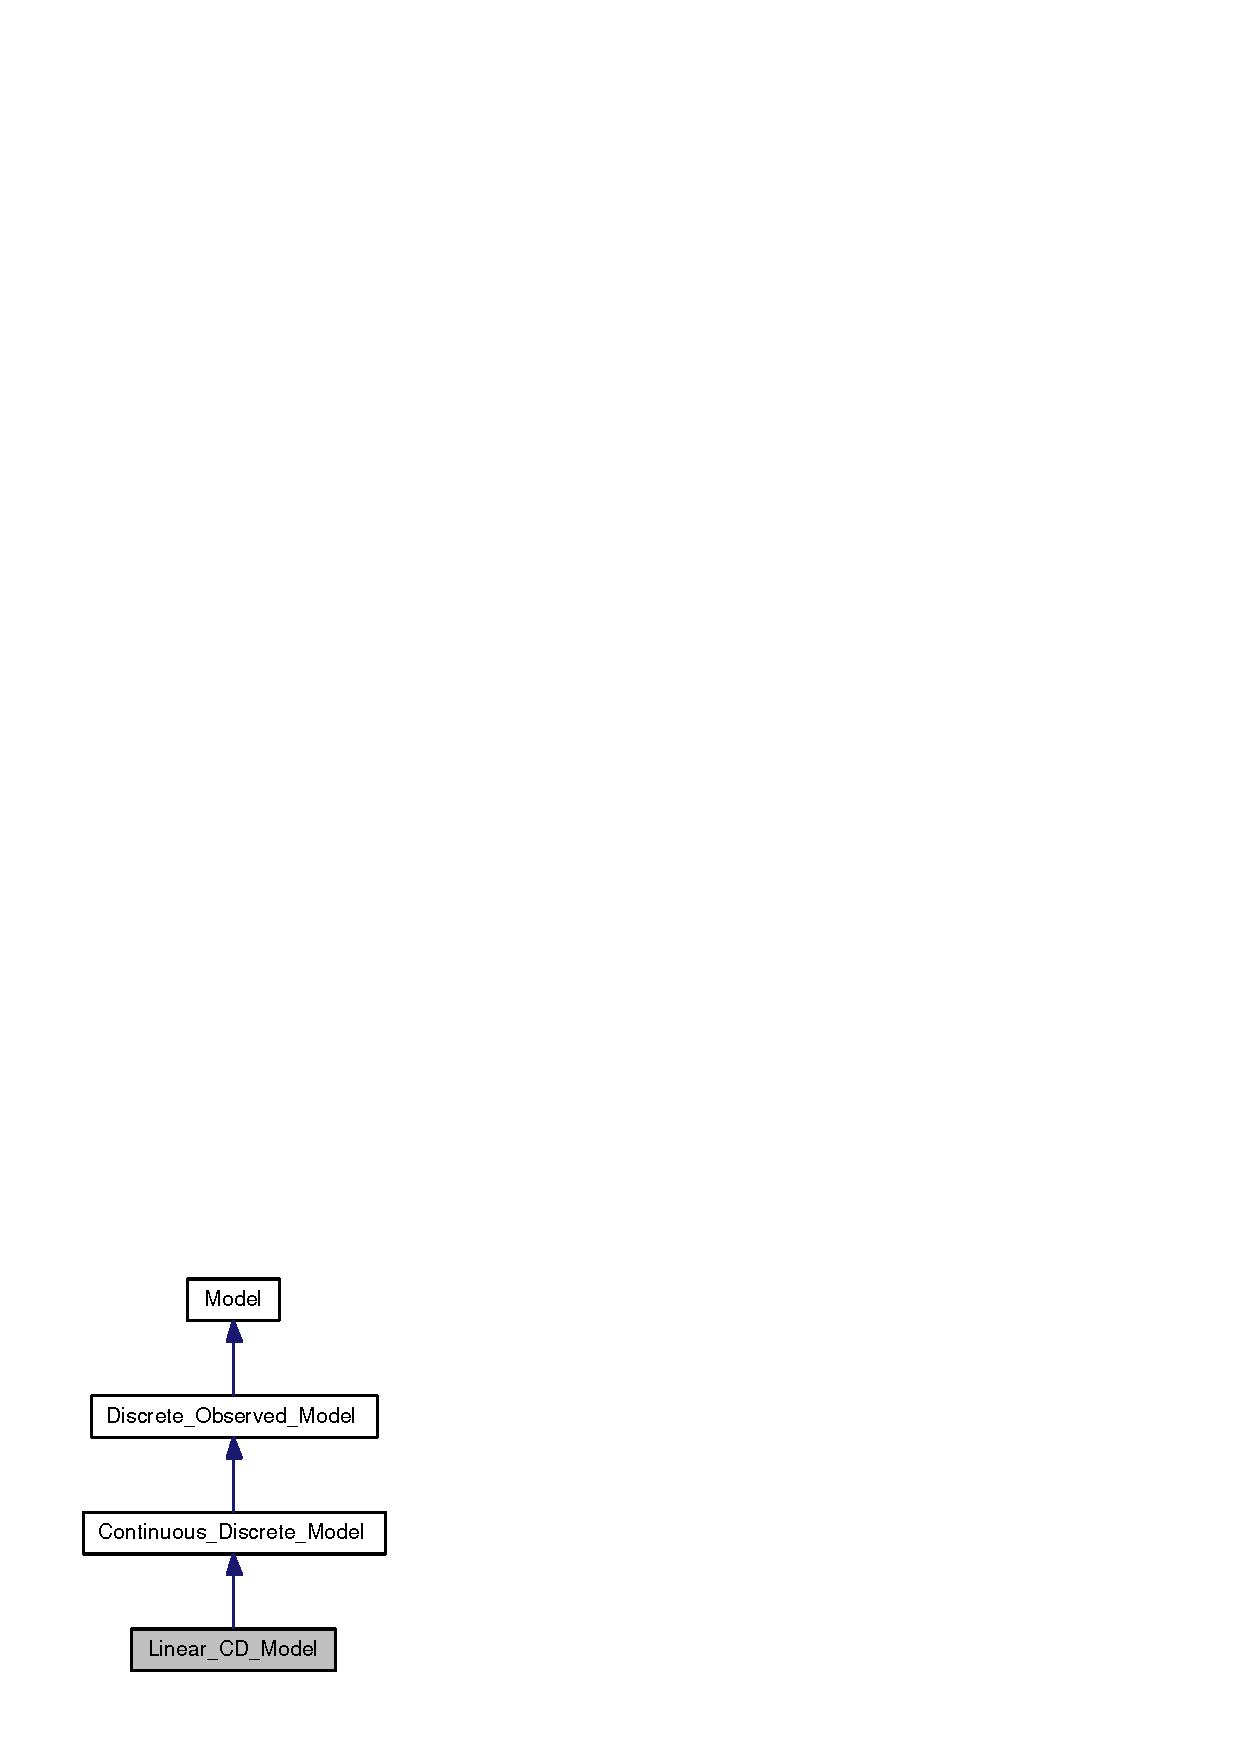
\includegraphics[width=94pt]{class_linear___c_d___model__inherit__graph}
\end{center}
\end{figure}
\subsection*{Public Member Functions}
\begin{CompactItemize}
\item 
\hyperlink{class_linear___c_d___model_aff713973f904c1a509373259ffb2275}{Linear\_\-CD\_\-Model} (void)
\item 
dcovector \hyperlink{class_linear___c_d___model_4a35ab32a6ff01885368d1b3690f4925}{Drift\_\-Function} (const dcovector \&X)
\begin{CompactList}\small\item\em the drift function of dX(t) = F(X)dt + G(X)$\ast$dW \item\end{CompactList}\item 
dgematrix \hyperlink{class_linear___c_d___model_6d063fdeaeba656c8449e1539f422e1a}{J\_\-Drift\_\-Function} (const dcovector \&X)
\begin{CompactList}\small\item\em the jacobian of the drift function evaluate at X \item\end{CompactList}\item 
dgematrix \hyperlink{class_linear___c_d___model_f6959eff1f30ff1772b05a45c5756054}{Diffusion\_\-Function} (void)
\begin{CompactList}\small\item\em the diffusion function \item\end{CompactList}\item 
dcovector \hyperlink{class_linear___c_d___model_79ddecd171ea3725ed37ea689e53bf96}{Observation\_\-Function} (const dcovector \&X)
\begin{CompactList}\small\item\em The observation Yk=H(Xk) + Vk. \item\end{CompactList}\item 
dgematrix \hyperlink{class_linear___c_d___model_6188317af5df5b7d495f84256bb1c75a}{J\_\-Observation\_\-Function} (const dcovector \&X)
\begin{CompactList}\small\item\em the jacobian of the observation function evaluate at X \item\end{CompactList}\item 
dcovector \hyperlink{class_linear___c_d___model_1aa9a1ed9415253e316342e7b24c9966}{Get\_\-Mean\_\-Prediction} (const dcovector \&M)
\item 
dgematrix \hyperlink{class_linear___c_d___model_8dd88775ae8db03490c423bbfb108440}{Get\_\-Cov\_\-Prediction} (const dgematrix \&P)
\item 
virtual void \hyperlink{class_linear___c_d___model_c115137cf3ae0d1670880d5a8b0a8bd4}{Init} (void)
\end{CompactItemize}
\subsection*{Public Attributes}
\begin{CompactItemize}
\item 
dgematrix \hyperlink{class_linear___c_d___model_d64d1305f494961cffd5d66cb3d24402}{A}
\item 
dcovector \hyperlink{class_linear___c_d___model_57d5af4675a8f42aeefa2bd393b4a7a9}{B}
\item 
dgematrix \hyperlink{class_linear___c_d___model_f2f4e6e226be8baf21fc70e83364a133}{C}
\item 
dcovector \hyperlink{class_linear___c_d___model_78bc761f7ba4b7046a16c73bc6397a86}{h}
\item 
dgematrix \hyperlink{class_linear___c_d___model_2627e7fc3df30be48f3836ebca15eb1d}{H}
\end{CompactItemize}


\subsection{Detailed Description}
Linear continuous discrete model class of the form dx = AX dt + Bdt + CdW Y\_\-k = HX(t\_\-k) + h + V\_\-k. 

\subsection{Constructor \& Destructor Documentation}
\hypertarget{class_linear___c_d___model_aff713973f904c1a509373259ffb2275}{
\index{Linear\_\-CD\_\-Model@{Linear\_\-CD\_\-Model}!Linear\_\-CD\_\-Model@{Linear\_\-CD\_\-Model}}
\index{Linear\_\-CD\_\-Model@{Linear\_\-CD\_\-Model}!Linear_CD_Model@{Linear\_\-CD\_\-Model}}
\subsubsection[{Linear\_\-CD\_\-Model}]{\setlength{\rightskip}{0pt plus 5cm}Linear\_\-CD\_\-Model::Linear\_\-CD\_\-Model (void)}}
\label{class_linear___c_d___model_aff713973f904c1a509373259ffb2275}




\subsection{Member Function Documentation}
\hypertarget{class_linear___c_d___model_f6959eff1f30ff1772b05a45c5756054}{
\index{Linear\_\-CD\_\-Model@{Linear\_\-CD\_\-Model}!Diffusion\_\-Function@{Diffusion\_\-Function}}
\index{Diffusion\_\-Function@{Diffusion\_\-Function}!Linear_CD_Model@{Linear\_\-CD\_\-Model}}
\subsubsection[{Diffusion\_\-Function}]{\setlength{\rightskip}{0pt plus 5cm}dgematrix Linear\_\-CD\_\-Model::Diffusion\_\-Function (void)\hspace{0.3cm}{\tt  \mbox{[}virtual\mbox{]}}}}
\label{class_linear___c_d___model_f6959eff1f30ff1772b05a45c5756054}


the diffusion function 

\begin{Desc}
\item[Parameters:]
\begin{description}
\item[{\em X}]the state\end{description}
\end{Desc}
\begin{Desc}
\item[Returns:]G(X). \end{Desc}


Implements \hyperlink{class_continuous___discrete___model_e305ba43f31be1275ede8d3d48d1d779}{Continuous\_\-Discrete\_\-Model}.\hypertarget{class_linear___c_d___model_4a35ab32a6ff01885368d1b3690f4925}{
\index{Linear\_\-CD\_\-Model@{Linear\_\-CD\_\-Model}!Drift\_\-Function@{Drift\_\-Function}}
\index{Drift\_\-Function@{Drift\_\-Function}!Linear_CD_Model@{Linear\_\-CD\_\-Model}}
\subsubsection[{Drift\_\-Function}]{\setlength{\rightskip}{0pt plus 5cm}dcovector Linear\_\-CD\_\-Model::Drift\_\-Function (const dcovector \& {\em X})\hspace{0.3cm}{\tt  \mbox{[}virtual\mbox{]}}}}
\label{class_linear___c_d___model_4a35ab32a6ff01885368d1b3690f4925}


the drift function of dX(t) = F(X)dt + G(X)$\ast$dW 

\begin{Desc}
\item[Parameters:]
\begin{description}
\item[{\em X}]the state.\end{description}
\end{Desc}
\begin{Desc}
\item[Returns:]f(X) \end{Desc}


Implements \hyperlink{class_continuous___discrete___model_fb901d0d92470ee3e2f5a06f74336b7d}{Continuous\_\-Discrete\_\-Model}.\hypertarget{class_linear___c_d___model_8dd88775ae8db03490c423bbfb108440}{
\index{Linear\_\-CD\_\-Model@{Linear\_\-CD\_\-Model}!Get\_\-Cov\_\-Prediction@{Get\_\-Cov\_\-Prediction}}
\index{Get\_\-Cov\_\-Prediction@{Get\_\-Cov\_\-Prediction}!Linear_CD_Model@{Linear\_\-CD\_\-Model}}
\subsubsection[{Get\_\-Cov\_\-Prediction}]{\setlength{\rightskip}{0pt plus 5cm}dgematrix Linear\_\-CD\_\-Model::Get\_\-Cov\_\-Prediction (const dgematrix \& {\em P})}}
\label{class_linear___c_d___model_8dd88775ae8db03490c423bbfb108440}


\hypertarget{class_linear___c_d___model_1aa9a1ed9415253e316342e7b24c9966}{
\index{Linear\_\-CD\_\-Model@{Linear\_\-CD\_\-Model}!Get\_\-Mean\_\-Prediction@{Get\_\-Mean\_\-Prediction}}
\index{Get\_\-Mean\_\-Prediction@{Get\_\-Mean\_\-Prediction}!Linear_CD_Model@{Linear\_\-CD\_\-Model}}
\subsubsection[{Get\_\-Mean\_\-Prediction}]{\setlength{\rightskip}{0pt plus 5cm}dcovector Linear\_\-CD\_\-Model::Get\_\-Mean\_\-Prediction (const dcovector \& {\em M})}}
\label{class_linear___c_d___model_1aa9a1ed9415253e316342e7b24c9966}


\hypertarget{class_linear___c_d___model_c115137cf3ae0d1670880d5a8b0a8bd4}{
\index{Linear\_\-CD\_\-Model@{Linear\_\-CD\_\-Model}!Init@{Init}}
\index{Init@{Init}!Linear_CD_Model@{Linear\_\-CD\_\-Model}}
\subsubsection[{Init}]{\setlength{\rightskip}{0pt plus 5cm}virtual void Linear\_\-CD\_\-Model::Init (void)\hspace{0.3cm}{\tt  \mbox{[}inline, virtual\mbox{]}}}}
\label{class_linear___c_d___model_c115137cf3ae0d1670880d5a8b0a8bd4}


Initialized CD model 

Reimplemented from \hyperlink{class_continuous___discrete___model_fb787d768352c5a38048c35e51e7735d}{Continuous\_\-Discrete\_\-Model}.\hypertarget{class_linear___c_d___model_6d063fdeaeba656c8449e1539f422e1a}{
\index{Linear\_\-CD\_\-Model@{Linear\_\-CD\_\-Model}!J\_\-Drift\_\-Function@{J\_\-Drift\_\-Function}}
\index{J\_\-Drift\_\-Function@{J\_\-Drift\_\-Function}!Linear_CD_Model@{Linear\_\-CD\_\-Model}}
\subsubsection[{J\_\-Drift\_\-Function}]{\setlength{\rightskip}{0pt plus 5cm}dgematrix Linear\_\-CD\_\-Model::J\_\-Drift\_\-Function (const dcovector \& {\em X})\hspace{0.3cm}{\tt  \mbox{[}virtual\mbox{]}}}}
\label{class_linear___c_d___model_6d063fdeaeba656c8449e1539f422e1a}


the jacobian of the drift function evaluate at X 

\begin{Desc}
\item[Parameters:]
\begin{description}
\item[{\em X}]\end{description}
\end{Desc}
\begin{Desc}
\item[Returns:]the jacobian matrix \end{Desc}


Reimplemented from \hyperlink{class_continuous___discrete___model_634d515a19cc782505935c8f23b00fff}{Continuous\_\-Discrete\_\-Model}.\hypertarget{class_linear___c_d___model_6188317af5df5b7d495f84256bb1c75a}{
\index{Linear\_\-CD\_\-Model@{Linear\_\-CD\_\-Model}!J\_\-Observation\_\-Function@{J\_\-Observation\_\-Function}}
\index{J\_\-Observation\_\-Function@{J\_\-Observation\_\-Function}!Linear_CD_Model@{Linear\_\-CD\_\-Model}}
\subsubsection[{J\_\-Observation\_\-Function}]{\setlength{\rightskip}{0pt plus 5cm}dgematrix Linear\_\-CD\_\-Model::J\_\-Observation\_\-Function (const dcovector \& {\em X})\hspace{0.3cm}{\tt  \mbox{[}virtual\mbox{]}}}}
\label{class_linear___c_d___model_6188317af5df5b7d495f84256bb1c75a}


the jacobian of the observation function evaluate at X 

\begin{Desc}
\item[Parameters:]
\begin{description}
\item[{\em X}]\end{description}
\end{Desc}
\begin{Desc}
\item[Returns:]The jacobian matrix \end{Desc}


Reimplemented from \hyperlink{class_discrete___observed___model_83cd1f2f54544d8977dbce844031f85e}{Discrete\_\-Observed\_\-Model}.\hypertarget{class_linear___c_d___model_79ddecd171ea3725ed37ea689e53bf96}{
\index{Linear\_\-CD\_\-Model@{Linear\_\-CD\_\-Model}!Observation\_\-Function@{Observation\_\-Function}}
\index{Observation\_\-Function@{Observation\_\-Function}!Linear_CD_Model@{Linear\_\-CD\_\-Model}}
\subsubsection[{Observation\_\-Function}]{\setlength{\rightskip}{0pt plus 5cm}dcovector Linear\_\-CD\_\-Model::Observation\_\-Function (const dcovector \& {\em X})\hspace{0.3cm}{\tt  \mbox{[}virtual\mbox{]}}}}
\label{class_linear___c_d___model_79ddecd171ea3725ed37ea689e53bf96}


The observation Yk=H(Xk) + Vk. 

\begin{Desc}
\item[Parameters:]
\begin{description}
\item[{\em X}]The state at k\end{description}
\end{Desc}
\begin{Desc}
\item[Returns:]The observation at k \end{Desc}


Implements \hyperlink{class_discrete___observed___model_8d56d86ea6b204672c8ebd720f1e11a6}{Discrete\_\-Observed\_\-Model}.

\subsection{Member Data Documentation}
\hypertarget{class_linear___c_d___model_d64d1305f494961cffd5d66cb3d24402}{
\index{Linear\_\-CD\_\-Model@{Linear\_\-CD\_\-Model}!A@{A}}
\index{A@{A}!Linear_CD_Model@{Linear\_\-CD\_\-Model}}
\subsubsection[{A}]{\setlength{\rightskip}{0pt plus 5cm}dgematrix {\bf Linear\_\-CD\_\-Model::A}}}
\label{class_linear___c_d___model_d64d1305f494961cffd5d66cb3d24402}


\hypertarget{class_linear___c_d___model_57d5af4675a8f42aeefa2bd393b4a7a9}{
\index{Linear\_\-CD\_\-Model@{Linear\_\-CD\_\-Model}!B@{B}}
\index{B@{B}!Linear_CD_Model@{Linear\_\-CD\_\-Model}}
\subsubsection[{B}]{\setlength{\rightskip}{0pt plus 5cm}dcovector {\bf Linear\_\-CD\_\-Model::B}}}
\label{class_linear___c_d___model_57d5af4675a8f42aeefa2bd393b4a7a9}


\hypertarget{class_linear___c_d___model_f2f4e6e226be8baf21fc70e83364a133}{
\index{Linear\_\-CD\_\-Model@{Linear\_\-CD\_\-Model}!C@{C}}
\index{C@{C}!Linear_CD_Model@{Linear\_\-CD\_\-Model}}
\subsubsection[{C}]{\setlength{\rightskip}{0pt plus 5cm}dgematrix {\bf Linear\_\-CD\_\-Model::C}}}
\label{class_linear___c_d___model_f2f4e6e226be8baf21fc70e83364a133}


\hypertarget{class_linear___c_d___model_2627e7fc3df30be48f3836ebca15eb1d}{
\index{Linear\_\-CD\_\-Model@{Linear\_\-CD\_\-Model}!H@{H}}
\index{H@{H}!Linear_CD_Model@{Linear\_\-CD\_\-Model}}
\subsubsection[{H}]{\setlength{\rightskip}{0pt plus 5cm}dgematrix {\bf Linear\_\-CD\_\-Model::H}}}
\label{class_linear___c_d___model_2627e7fc3df30be48f3836ebca15eb1d}


\hypertarget{class_linear___c_d___model_78bc761f7ba4b7046a16c73bc6397a86}{
\index{Linear\_\-CD\_\-Model@{Linear\_\-CD\_\-Model}!h@{h}}
\index{h@{h}!Linear_CD_Model@{Linear\_\-CD\_\-Model}}
\subsubsection[{h}]{\setlength{\rightskip}{0pt plus 5cm}dcovector {\bf Linear\_\-CD\_\-Model::h}}}
\label{class_linear___c_d___model_78bc761f7ba4b7046a16c73bc6397a86}



\hypertarget{class_l_l___filter}{
\section{LL\_\-Filter Class Reference}
\label{class_l_l___filter}\index{LL\_\-Filter@{LL\_\-Filter}}
}
{\tt \#include $<$local\_\-linearization\_\-filter.h$>$}

Inheritance diagram for LL\_\-Filter:\nopagebreak
\begin{figure}[H]
\begin{center}
\leavevmode
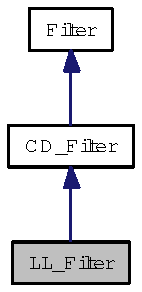
\includegraphics[width=52pt]{class_l_l___filter__inherit__graph}
\end{center}
\end{figure}
\subsection*{Public Member Functions}
\begin{CompactItemize}
\item 
\hyperlink{class_l_l___filter_b8180cc8e1c5e0c1199acced77b3609f}{LL\_\-Filter} (void)
\item 
\hyperlink{class_l_l___filter_a05b72bc41b502dea8abcafc7ff95384}{LL\_\-Filter} (\hyperlink{class_continuous___discrete___model}{Continuous\_\-Discrete\_\-Model} $\ast$m)
\end{CompactItemize}
\subsection*{Protected Member Functions}
\begin{CompactItemize}
\item 
int \hyperlink{class_l_l___filter_ab2b4b545d401d54c66f63a41fa1a99d}{\_\-update} (const dcovector \&Y)
\end{CompactItemize}


\subsection{Constructor \& Destructor Documentation}
\hypertarget{class_l_l___filter_b8180cc8e1c5e0c1199acced77b3609f}{
\index{LL\_\-Filter@{LL\_\-Filter}!LL\_\-Filter@{LL\_\-Filter}}
\index{LL\_\-Filter@{LL\_\-Filter}!LL_Filter@{LL\_\-Filter}}
\subsubsection[{LL\_\-Filter}]{\setlength{\rightskip}{0pt plus 5cm}LL\_\-Filter::LL\_\-Filter (void)}}
\label{class_l_l___filter_b8180cc8e1c5e0c1199acced77b3609f}


\hypertarget{class_l_l___filter_a05b72bc41b502dea8abcafc7ff95384}{
\index{LL\_\-Filter@{LL\_\-Filter}!LL\_\-Filter@{LL\_\-Filter}}
\index{LL\_\-Filter@{LL\_\-Filter}!LL_Filter@{LL\_\-Filter}}
\subsubsection[{LL\_\-Filter}]{\setlength{\rightskip}{0pt plus 5cm}LL\_\-Filter::LL\_\-Filter ({\bf Continuous\_\-Discrete\_\-Model} $\ast$ {\em m})}}
\label{class_l_l___filter_a05b72bc41b502dea8abcafc7ff95384}




\subsection{Member Function Documentation}
\hypertarget{class_l_l___filter_ab2b4b545d401d54c66f63a41fa1a99d}{
\index{LL\_\-Filter@{LL\_\-Filter}!\_\-update@{\_\-update}}
\index{\_\-update@{\_\-update}!LL_Filter@{LL\_\-Filter}}
\subsubsection[{\_\-update}]{\setlength{\rightskip}{0pt plus 5cm}int LL\_\-Filter::\_\-update (const dcovector \& {\em Y})\hspace{0.3cm}{\tt  \mbox{[}protected, virtual\mbox{]}}}}
\label{class_l_l___filter_ab2b4b545d401d54c66f63a41fa1a99d}


Specific update for each filter

\begin{Desc}
\item[Parameters:]
\begin{description}
\item[{\em Y}]The observed sample\end{description}
\end{Desc}
\begin{Desc}
\item[Returns:]0 if no problem \end{Desc}


Implements \hyperlink{class_filter_20ecd17fed3b8f11a76c960fe5e7144b}{Filter}.
\hypertarget{class_l_t_i___c_d___simulator}{
\section{LTI\_\-CD\_\-Simulator Class Reference}
\label{class_l_t_i___c_d___simulator}\index{LTI\_\-CD\_\-Simulator@{LTI\_\-CD\_\-Simulator}}
}
{\tt \#include $<$simulator.h$>$}

Inheritance diagram for LTI\_\-CD\_\-Simulator:\nopagebreak
\begin{figure}[H]
\begin{center}
\leavevmode
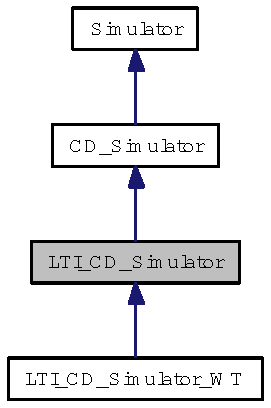
\includegraphics[width=83pt]{class_l_t_i___c_d___simulator__inherit__graph}
\end{center}
\end{figure}
\subsection*{Public Member Functions}
\begin{CompactItemize}
\item 
\hyperlink{class_l_t_i___c_d___simulator_86b38b889838a1efdec15f1f18fd55f3}{LTI\_\-CD\_\-Simulator} (void)
\item 
\hyperlink{class_l_t_i___c_d___simulator_3126a80b8ca7eaec68232e470d0c0595}{LTI\_\-CD\_\-Simulator} (\hyperlink{class_linear___c_d___model}{Linear\_\-CD\_\-Model} $\ast$cd\_\-m, const int \&apha=1)
\end{CompactItemize}
\subsection*{Protected Member Functions}
\begin{CompactItemize}
\item 
dcovector \hyperlink{class_l_t_i___c_d___simulator_1497e233ff1a0d71c2b660fe270c9ff8}{draw\_\-state} (const dcovector \&\hyperlink{class_simulator_a2db8ace19099d996be516022d230bc0}{X})
\end{CompactItemize}


\subsection{Constructor \& Destructor Documentation}
\hypertarget{class_l_t_i___c_d___simulator_86b38b889838a1efdec15f1f18fd55f3}{
\index{LTI\_\-CD\_\-Simulator@{LTI\_\-CD\_\-Simulator}!LTI\_\-CD\_\-Simulator@{LTI\_\-CD\_\-Simulator}}
\index{LTI\_\-CD\_\-Simulator@{LTI\_\-CD\_\-Simulator}!LTI_CD_Simulator@{LTI\_\-CD\_\-Simulator}}
\subsubsection[{LTI\_\-CD\_\-Simulator}]{\setlength{\rightskip}{0pt plus 5cm}LTI\_\-CD\_\-Simulator::LTI\_\-CD\_\-Simulator (void)}}
\label{class_l_t_i___c_d___simulator_86b38b889838a1efdec15f1f18fd55f3}


\hypertarget{class_l_t_i___c_d___simulator_3126a80b8ca7eaec68232e470d0c0595}{
\index{LTI\_\-CD\_\-Simulator@{LTI\_\-CD\_\-Simulator}!LTI\_\-CD\_\-Simulator@{LTI\_\-CD\_\-Simulator}}
\index{LTI\_\-CD\_\-Simulator@{LTI\_\-CD\_\-Simulator}!LTI_CD_Simulator@{LTI\_\-CD\_\-Simulator}}
\subsubsection[{LTI\_\-CD\_\-Simulator}]{\setlength{\rightskip}{0pt plus 5cm}LTI\_\-CD\_\-Simulator::LTI\_\-CD\_\-Simulator ({\bf Linear\_\-CD\_\-Model} $\ast$ {\em cd\_\-m}, \/  const int \& {\em apha} = {\tt 1})}}
\label{class_l_t_i___c_d___simulator_3126a80b8ca7eaec68232e470d0c0595}




\subsection{Member Function Documentation}
\hypertarget{class_l_t_i___c_d___simulator_1497e233ff1a0d71c2b660fe270c9ff8}{
\index{LTI\_\-CD\_\-Simulator@{LTI\_\-CD\_\-Simulator}!draw\_\-state@{draw\_\-state}}
\index{draw\_\-state@{draw\_\-state}!LTI_CD_Simulator@{LTI\_\-CD\_\-Simulator}}
\subsubsection[{draw\_\-state}]{\setlength{\rightskip}{0pt plus 5cm}dcovector LTI\_\-CD\_\-Simulator::draw\_\-state (const dcovector \& {\em X})\hspace{0.3cm}{\tt  \mbox{[}protected, virtual\mbox{]}}}}
\label{class_l_t_i___c_d___simulator_1497e233ff1a0d71c2b660fe270c9ff8}




Reimplemented from \hyperlink{class_c_d___simulator_11c411df9b1e0d6f8576edefd723dd47}{CD\_\-Simulator}.
\hypertarget{class_l_t_i___c_d___simulator___w_t}{
\section{LTI\_\-CD\_\-Simulator\_\-WT Class Reference}
\label{class_l_t_i___c_d___simulator___w_t}\index{LTI\_\-CD\_\-Simulator\_\-WT@{LTI\_\-CD\_\-Simulator\_\-WT}}
}
{\tt \#include $<$simulator.h$>$}

Inheritance diagram for LTI\_\-CD\_\-Simulator\_\-WT:\nopagebreak
\begin{figure}[H]
\begin{center}
\leavevmode
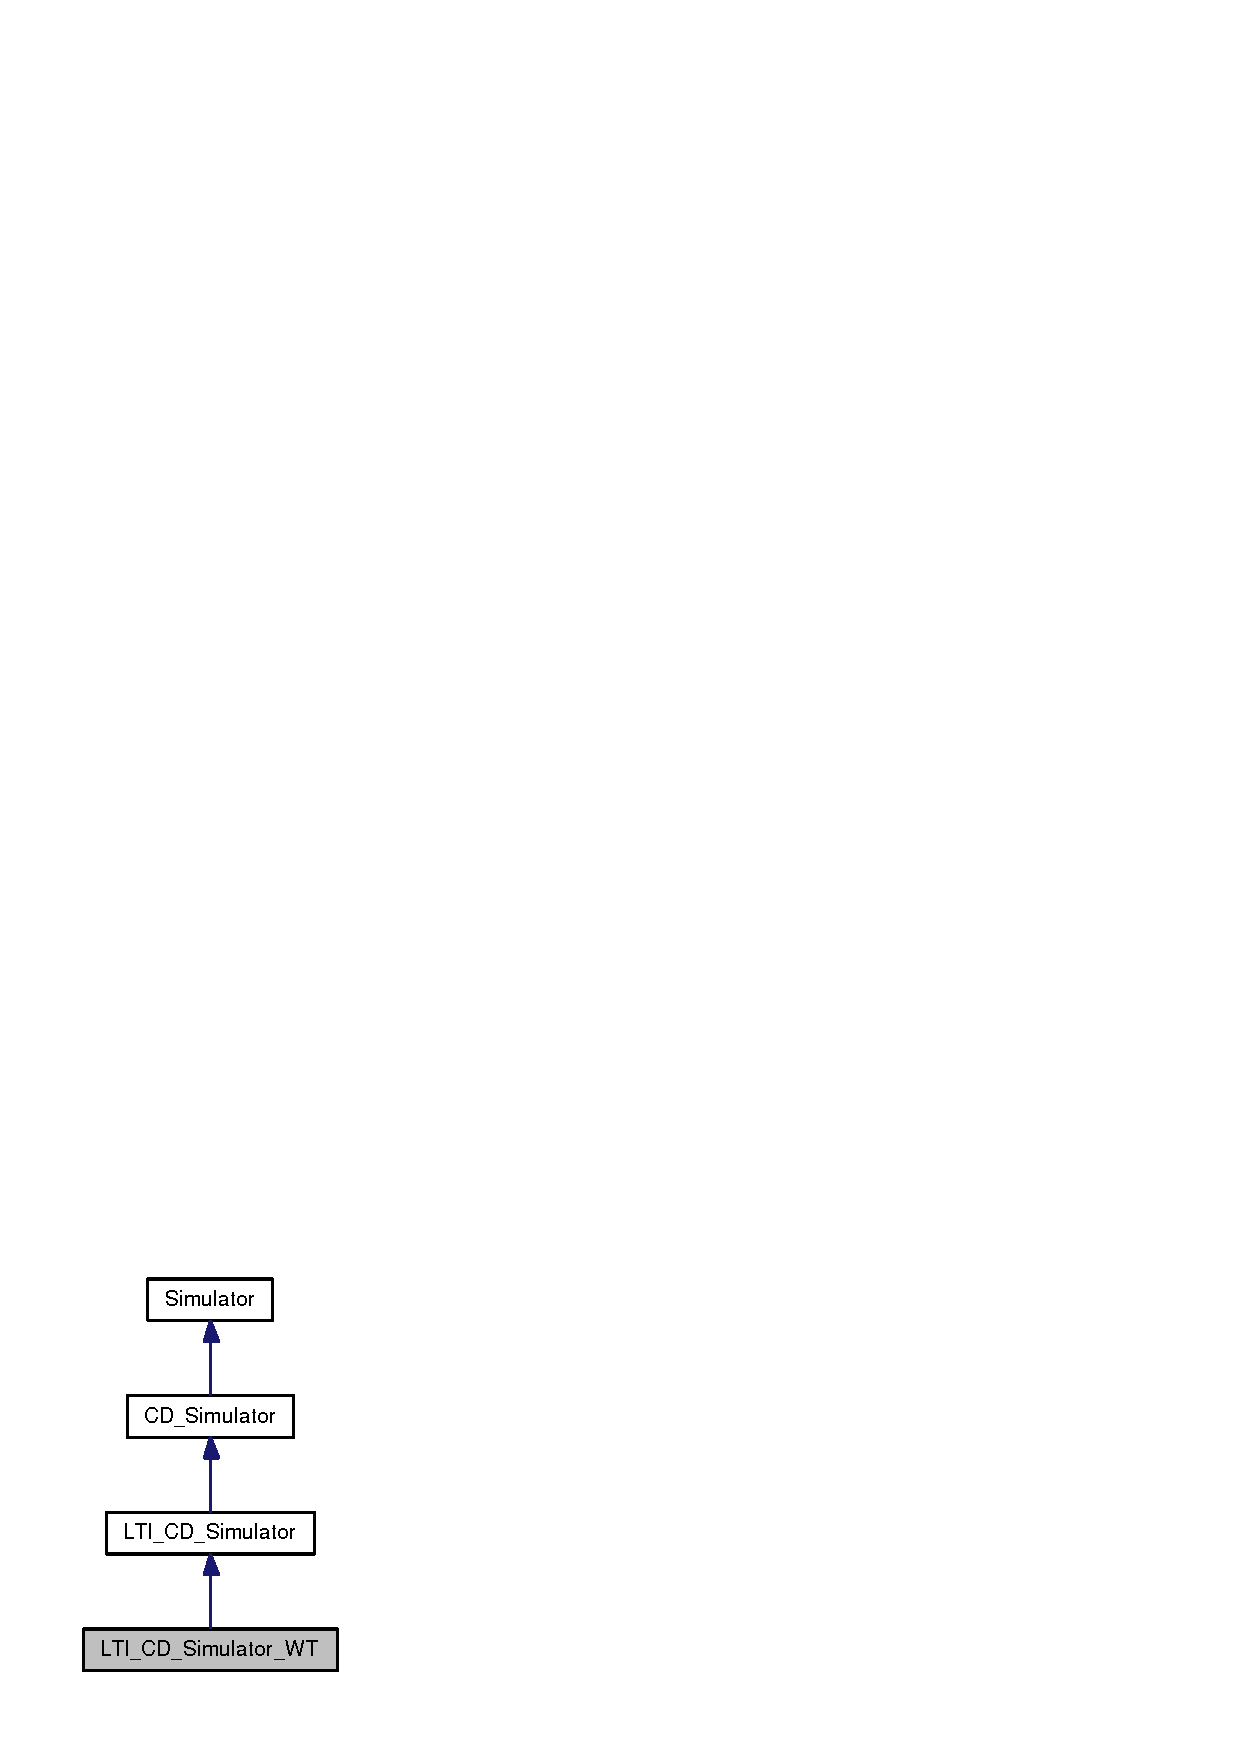
\includegraphics[width=83pt]{class_l_t_i___c_d___simulator___w_t__inherit__graph}
\end{center}
\end{figure}
\subsection*{Public Member Functions}
\begin{CompactItemize}
\item 
\hyperlink{class_l_t_i___c_d___simulator___w_t_b19915f3fc8903845fe748efd495fb5a}{LTI\_\-CD\_\-Simulator\_\-WT} (void)
\item 
\hyperlink{class_l_t_i___c_d___simulator___w_t_2d512981a1e18a2fab3e2ad7b5ea9b43}{LTI\_\-CD\_\-Simulator\_\-WT} (\hyperlink{class_linear___c_d___model}{Linear\_\-CD\_\-Model} $\ast$cd\_\-m, const int \&apha, const double \&tb, const double \&t)
\item 
dcovector \hyperlink{class_l_t_i___c_d___simulator___w_t_a63eaac608a5f214468dc13d34f8f20f}{Draw\_\-Init} (void)
\begin{CompactList}\small\item\em Draw a sample from p(X0). \item\end{CompactList}\end{CompactItemize}
\subsection*{Private Attributes}
\begin{CompactItemize}
\item 
vector$<$ dcovector $>$ \hyperlink{class_l_t_i___c_d___simulator___w_t_97dfbe7f66cefff7b32d3288aece9964}{Xt}
\item 
double \hyperlink{class_l_t_i___c_d___simulator___w_t_f03a9456dc6940c1c3f772336d911c3e}{TB}
\item 
double \hyperlink{class_l_t_i___c_d___simulator___w_t_5ceaf9896225588b2aff938b13e86996}{T}
\end{CompactItemize}


\subsection{Constructor \& Destructor Documentation}
\hypertarget{class_l_t_i___c_d___simulator___w_t_b19915f3fc8903845fe748efd495fb5a}{
\index{LTI\_\-CD\_\-Simulator\_\-WT@{LTI\_\-CD\_\-Simulator\_\-WT}!LTI\_\-CD\_\-Simulator\_\-WT@{LTI\_\-CD\_\-Simulator\_\-WT}}
\index{LTI\_\-CD\_\-Simulator\_\-WT@{LTI\_\-CD\_\-Simulator\_\-WT}!LTI_CD_Simulator_WT@{LTI\_\-CD\_\-Simulator\_\-WT}}
\subsubsection[{LTI\_\-CD\_\-Simulator\_\-WT}]{\setlength{\rightskip}{0pt plus 5cm}LTI\_\-CD\_\-Simulator\_\-WT::LTI\_\-CD\_\-Simulator\_\-WT (void)}}
\label{class_l_t_i___c_d___simulator___w_t_b19915f3fc8903845fe748efd495fb5a}


\hypertarget{class_l_t_i___c_d___simulator___w_t_2d512981a1e18a2fab3e2ad7b5ea9b43}{
\index{LTI\_\-CD\_\-Simulator\_\-WT@{LTI\_\-CD\_\-Simulator\_\-WT}!LTI\_\-CD\_\-Simulator\_\-WT@{LTI\_\-CD\_\-Simulator\_\-WT}}
\index{LTI\_\-CD\_\-Simulator\_\-WT@{LTI\_\-CD\_\-Simulator\_\-WT}!LTI_CD_Simulator_WT@{LTI\_\-CD\_\-Simulator\_\-WT}}
\subsubsection[{LTI\_\-CD\_\-Simulator\_\-WT}]{\setlength{\rightskip}{0pt plus 5cm}LTI\_\-CD\_\-Simulator\_\-WT::LTI\_\-CD\_\-Simulator\_\-WT ({\bf Linear\_\-CD\_\-Model} $\ast$ {\em cd\_\-m}, \/  const int \& {\em apha}, \/  const double \& {\em tb}, \/  const double \& {\em t})}}
\label{class_l_t_i___c_d___simulator___w_t_2d512981a1e18a2fab3e2ad7b5ea9b43}




\subsection{Member Function Documentation}
\hypertarget{class_l_t_i___c_d___simulator___w_t_a63eaac608a5f214468dc13d34f8f20f}{
\index{LTI\_\-CD\_\-Simulator\_\-WT@{LTI\_\-CD\_\-Simulator\_\-WT}!Draw\_\-Init@{Draw\_\-Init}}
\index{Draw\_\-Init@{Draw\_\-Init}!LTI_CD_Simulator_WT@{LTI\_\-CD\_\-Simulator\_\-WT}}
\subsubsection[{Draw\_\-Init}]{\setlength{\rightskip}{0pt plus 5cm}dcovector LTI\_\-CD\_\-Simulator\_\-WT::Draw\_\-Init (void)\hspace{0.3cm}{\tt  \mbox{[}virtual\mbox{]}}}}
\label{class_l_t_i___c_d___simulator___w_t_a63eaac608a5f214468dc13d34f8f20f}


Draw a sample from p(X0). 

\begin{Desc}
\item[Returns:]A sample from p(X0) \end{Desc}


Reimplemented from \hyperlink{class_c_d___simulator_cbdbea3e487026be0c032d2218d27b2b}{CD\_\-Simulator}.

\subsection{Member Data Documentation}
\hypertarget{class_l_t_i___c_d___simulator___w_t_5ceaf9896225588b2aff938b13e86996}{
\index{LTI\_\-CD\_\-Simulator\_\-WT@{LTI\_\-CD\_\-Simulator\_\-WT}!T@{T}}
\index{T@{T}!LTI_CD_Simulator_WT@{LTI\_\-CD\_\-Simulator\_\-WT}}
\subsubsection[{T}]{\setlength{\rightskip}{0pt plus 5cm}double {\bf LTI\_\-CD\_\-Simulator\_\-WT::T}\hspace{0.3cm}{\tt  \mbox{[}private\mbox{]}}}}
\label{class_l_t_i___c_d___simulator___w_t_5ceaf9896225588b2aff938b13e86996}


\hypertarget{class_l_t_i___c_d___simulator___w_t_f03a9456dc6940c1c3f772336d911c3e}{
\index{LTI\_\-CD\_\-Simulator\_\-WT@{LTI\_\-CD\_\-Simulator\_\-WT}!TB@{TB}}
\index{TB@{TB}!LTI_CD_Simulator_WT@{LTI\_\-CD\_\-Simulator\_\-WT}}
\subsubsection[{TB}]{\setlength{\rightskip}{0pt plus 5cm}double {\bf LTI\_\-CD\_\-Simulator\_\-WT::TB}\hspace{0.3cm}{\tt  \mbox{[}private\mbox{]}}}}
\label{class_l_t_i___c_d___simulator___w_t_f03a9456dc6940c1c3f772336d911c3e}


\hypertarget{class_l_t_i___c_d___simulator___w_t_97dfbe7f66cefff7b32d3288aece9964}{
\index{LTI\_\-CD\_\-Simulator\_\-WT@{LTI\_\-CD\_\-Simulator\_\-WT}!Xt@{Xt}}
\index{Xt@{Xt}!LTI_CD_Simulator_WT@{LTI\_\-CD\_\-Simulator\_\-WT}}
\subsubsection[{Xt}]{\setlength{\rightskip}{0pt plus 5cm}vector$<$dcovector$>$ {\bf LTI\_\-CD\_\-Simulator\_\-WT::Xt}\hspace{0.3cm}{\tt  \mbox{[}private\mbox{]}}}}
\label{class_l_t_i___c_d___simulator___w_t_97dfbe7f66cefff7b32d3288aece9964}



\hypertarget{class_model}{
\section{Model Class Reference}
\label{class_model}\index{Model@{Model}}
}
The class of time varying-models.  


{\tt \#include $<$gaussian\_\-model.h$>$}

Inheritance diagram for Model:\nopagebreak
\begin{figure}[H]
\begin{center}
\leavevmode
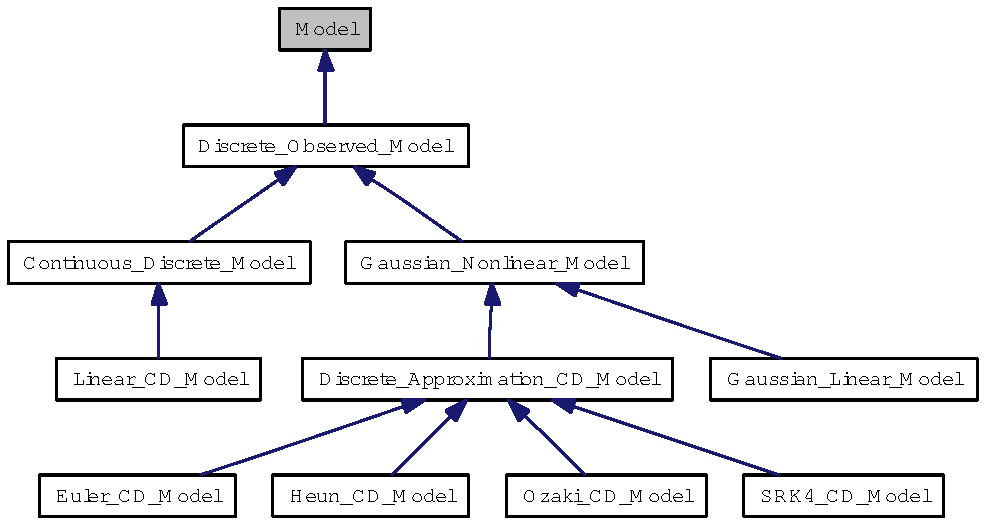
\includegraphics[width=400pt]{class_model__inherit__graph}
\end{center}
\end{figure}
\subsection*{Public Member Functions}
\begin{CompactItemize}
\item 
\hyperlink{class_model_a26cb9f39a3e0356152a57a2d2ecfaef}{Model} (void)
\item 
virtual \hyperlink{class_model_181e1dd7311fe966bf4f52c7feb592e4}{$\sim$Model} (void)
\begin{CompactList}\small\item\em The Destructor. \item\end{CompactList}\item 
int \hyperlink{class_model_e51159f212efa0af4b7c95a3d81e65db}{Update} (void)
\begin{CompactList}\small\item\em Update the time. \item\end{CompactList}\item 
int \hyperlink{class_model_fbf71c4ac9a04974625c7e1307e7d153}{Clear} (void)
\begin{CompactList}\small\item\em Set the time to 0. \item\end{CompactList}\item 
int \hyperlink{class_model_efbca8bb1098349a9c4c3ccfbba02aa2}{Get\_\-Time} (void)
\begin{CompactList}\small\item\em Get The current time. \item\end{CompactList}\end{CompactItemize}
\subsection*{Protected Attributes}
\begin{CompactItemize}
\item 
int \hyperlink{class_model_7bacdb5f50e67614833eacb6df7d68e9}{\_\-k}
\begin{CompactList}\small\item\em The time. \item\end{CompactList}\end{CompactItemize}


\subsection{Detailed Description}
The class of time varying-models. 



\subsection{Constructor \& Destructor Documentation}
\hypertarget{class_model_a26cb9f39a3e0356152a57a2d2ecfaef}{
\index{Model@{Model}!Model@{Model}}
\index{Model@{Model}!Model@{Model}}
\subsubsection[{Model}]{\setlength{\rightskip}{0pt plus 5cm}Model::Model (void)}}
\label{class_model_a26cb9f39a3e0356152a57a2d2ecfaef}


\hypertarget{class_model_181e1dd7311fe966bf4f52c7feb592e4}{
\index{Model@{Model}!$\sim$Model@{$\sim$Model}}
\index{$\sim$Model@{$\sim$Model}!Model@{Model}}
\subsubsection[{$\sim$Model}]{\setlength{\rightskip}{0pt plus 5cm}virtual Model::$\sim$Model (void)\hspace{0.3cm}{\tt  \mbox{[}virtual\mbox{]}}}}
\label{class_model_181e1dd7311fe966bf4f52c7feb592e4}


The Destructor. 

\begin{Desc}
\item[Returns:]\end{Desc}


\subsection{Member Function Documentation}
\hypertarget{class_model_fbf71c4ac9a04974625c7e1307e7d153}{
\index{Model@{Model}!Clear@{Clear}}
\index{Clear@{Clear}!Model@{Model}}
\subsubsection[{Clear}]{\setlength{\rightskip}{0pt plus 5cm}int Model::Clear (void)}}
\label{class_model_fbf71c4ac9a04974625c7e1307e7d153}


Set the time to 0. 

\begin{Desc}
\item[Returns:]0 if it's Ok; \end{Desc}
\hypertarget{class_model_efbca8bb1098349a9c4c3ccfbba02aa2}{
\index{Model@{Model}!Get\_\-Time@{Get\_\-Time}}
\index{Get\_\-Time@{Get\_\-Time}!Model@{Model}}
\subsubsection[{Get\_\-Time}]{\setlength{\rightskip}{0pt plus 5cm}int Model::Get\_\-Time (void)}}
\label{class_model_efbca8bb1098349a9c4c3ccfbba02aa2}


Get The current time. 

\begin{Desc}
\item[Returns:]\end{Desc}
\hypertarget{class_model_e51159f212efa0af4b7c95a3d81e65db}{
\index{Model@{Model}!Update@{Update}}
\index{Update@{Update}!Model@{Model}}
\subsubsection[{Update}]{\setlength{\rightskip}{0pt plus 5cm}int Model::Update (void)}}
\label{class_model_e51159f212efa0af4b7c95a3d81e65db}


Update the time. 

\begin{Desc}
\item[Returns:]0 if it's Ok; \end{Desc}


\subsection{Member Data Documentation}
\hypertarget{class_model_7bacdb5f50e67614833eacb6df7d68e9}{
\index{Model@{Model}!\_\-k@{\_\-k}}
\index{\_\-k@{\_\-k}!Model@{Model}}
\subsubsection[{\_\-k}]{\setlength{\rightskip}{0pt plus 5cm}int {\bf Model::\_\-k}\hspace{0.3cm}{\tt  \mbox{[}protected\mbox{]}}}}
\label{class_model_7bacdb5f50e67614833eacb6df7d68e9}


The time. 


\hypertarget{class_opt___simulator}{
\section{Opt\_\-Simulator Class Reference}
\label{class_opt___simulator}\index{Opt\_\-Simulator@{Opt\_\-Simulator}}
}
{\tt \#include $<$simulator.h$>$}

Inheritance diagram for Opt\_\-Simulator:\nopagebreak
\begin{figure}[H]
\begin{center}
\leavevmode
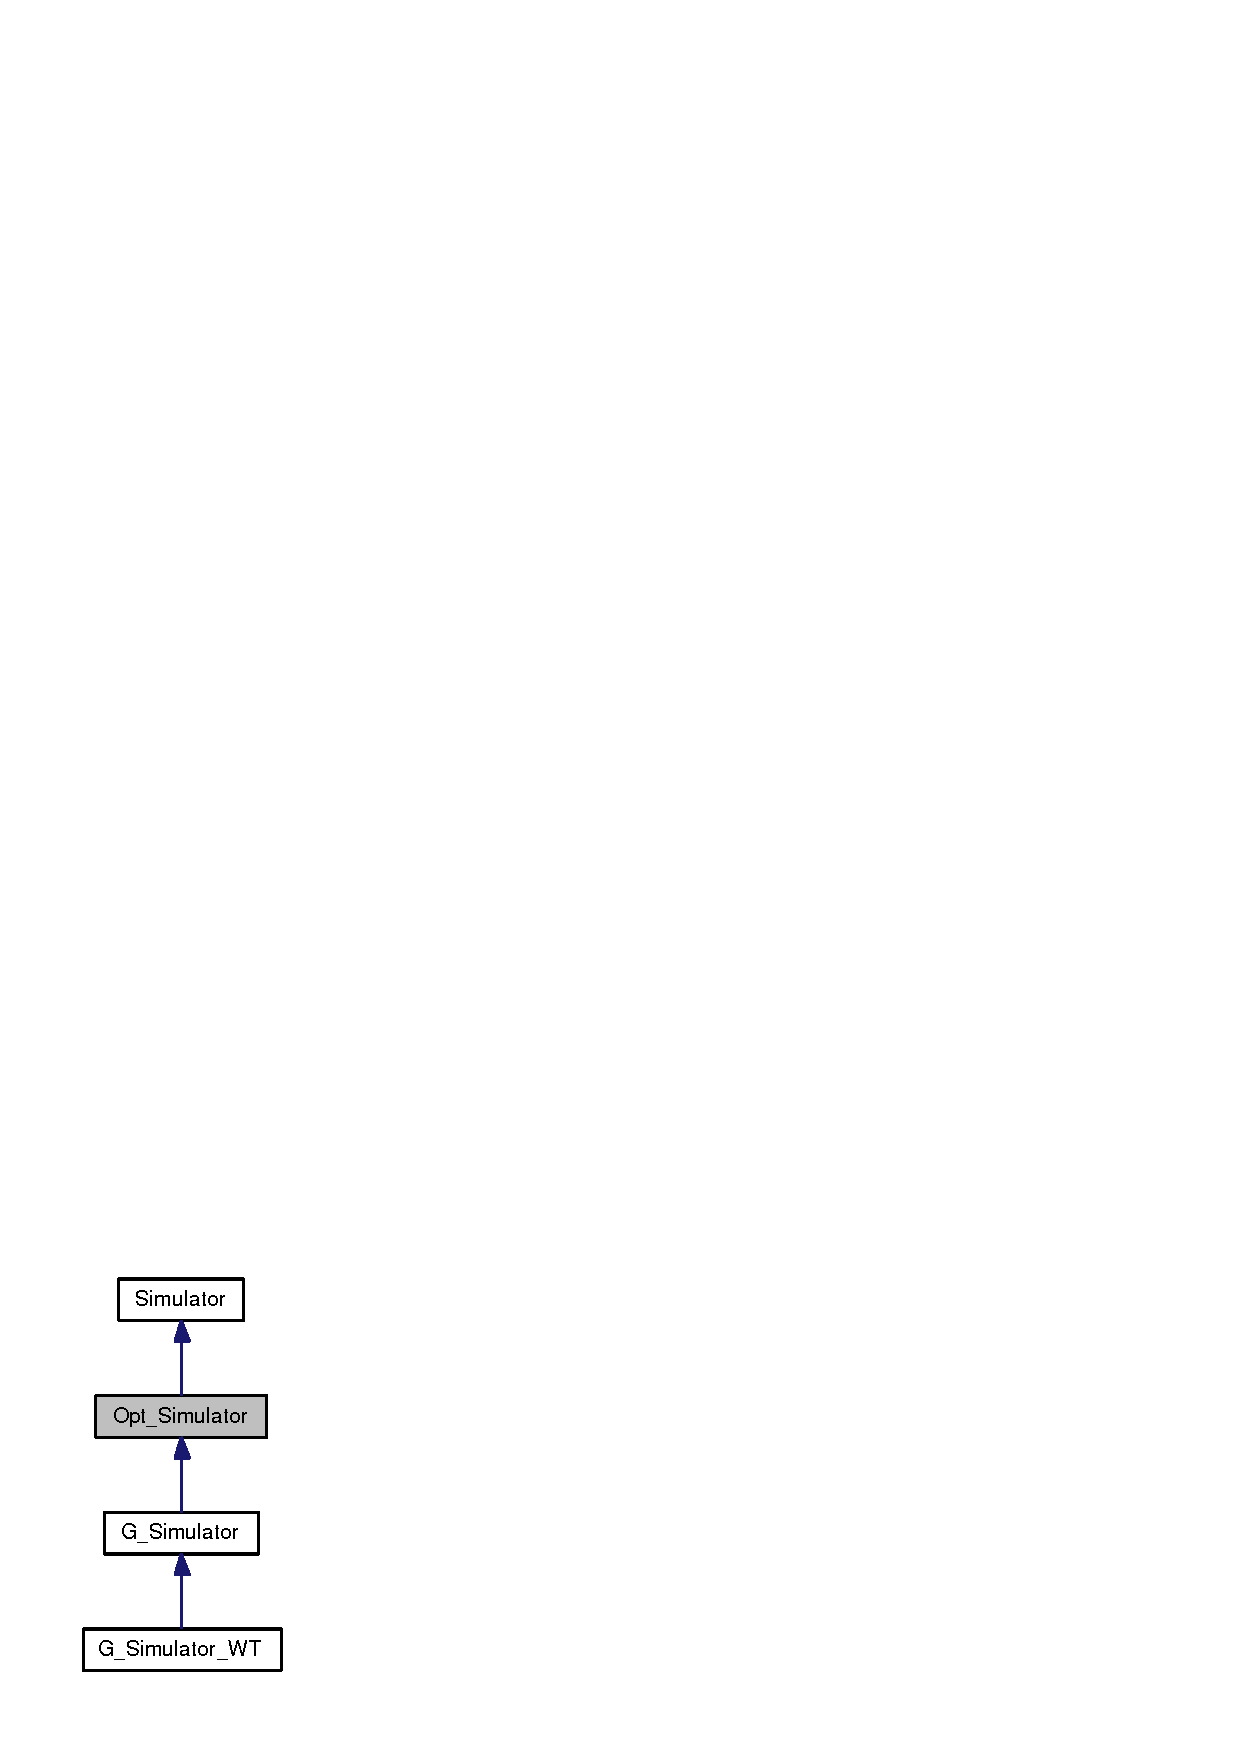
\includegraphics[width=69pt]{class_opt___simulator__inherit__graph}
\end{center}
\end{figure}
\subsection*{Public Member Functions}
\begin{CompactItemize}
\item 
\hyperlink{class_opt___simulator_9c18baf105bd365af92a933e1a068c3e}{Opt\_\-Simulator} (void)
\item 
virtual dcovector \hyperlink{class_opt___simulator_75490247df4dfa14eb7b2d8d394675dd}{Draw\_\-Optimal} (const dcovector \&Yk, const dcovector \&Xkm1)=0
\begin{CompactList}\small\item\em Draw a sample from the optimal densisty p(Xk$|$Yk,Xk-1). \item\end{CompactList}\item 
virtual long double \hyperlink{class_opt___simulator_e72d4709998087317635a94c709d71ba}{Obs\_\-Optimal\_\-Density} (const dcovector \&Yk, const dcovector \&Xkm1)=0
\begin{CompactList}\small\item\em calculate the value of the density of probability of Yk given Xk-1 : p(Yk$|$Xk-1) \item\end{CompactList}\end{CompactItemize}


\subsection{Constructor \& Destructor Documentation}
\hypertarget{class_opt___simulator_9c18baf105bd365af92a933e1a068c3e}{
\index{Opt\_\-Simulator@{Opt\_\-Simulator}!Opt\_\-Simulator@{Opt\_\-Simulator}}
\index{Opt\_\-Simulator@{Opt\_\-Simulator}!Opt_Simulator@{Opt\_\-Simulator}}
\subsubsection[{Opt\_\-Simulator}]{\setlength{\rightskip}{0pt plus 5cm}Opt\_\-Simulator::Opt\_\-Simulator (void)}}
\label{class_opt___simulator_9c18baf105bd365af92a933e1a068c3e}




\subsection{Member Function Documentation}
\hypertarget{class_opt___simulator_75490247df4dfa14eb7b2d8d394675dd}{
\index{Opt\_\-Simulator@{Opt\_\-Simulator}!Draw\_\-Optimal@{Draw\_\-Optimal}}
\index{Draw\_\-Optimal@{Draw\_\-Optimal}!Opt_Simulator@{Opt\_\-Simulator}}
\subsubsection[{Draw\_\-Optimal}]{\setlength{\rightskip}{0pt plus 5cm}virtual dcovector Opt\_\-Simulator::Draw\_\-Optimal (const dcovector \& {\em Yk}, \/  const dcovector \& {\em Xkm1})\hspace{0.3cm}{\tt  \mbox{[}pure virtual\mbox{]}}}}
\label{class_opt___simulator_75490247df4dfa14eb7b2d8d394675dd}


Draw a sample from the optimal densisty p(Xk$|$Yk,Xk-1). 

\begin{Desc}
\item[Parameters:]
\begin{description}
\item[{\em Yk}]The obseration at k \item[{\em Xkm1}]X(k-1) the state value at k-1\end{description}
\end{Desc}
\begin{Desc}
\item[Returns:]A sample from the optimal importance density \end{Desc}


Implemented in \hyperlink{class_g___simulator_b6c78e1dfa62c8c684b860ea1918f045}{G\_\-Simulator}.\hypertarget{class_opt___simulator_e72d4709998087317635a94c709d71ba}{
\index{Opt\_\-Simulator@{Opt\_\-Simulator}!Obs\_\-Optimal\_\-Density@{Obs\_\-Optimal\_\-Density}}
\index{Obs\_\-Optimal\_\-Density@{Obs\_\-Optimal\_\-Density}!Opt_Simulator@{Opt\_\-Simulator}}
\subsubsection[{Obs\_\-Optimal\_\-Density}]{\setlength{\rightskip}{0pt plus 5cm}virtual long double Opt\_\-Simulator::Obs\_\-Optimal\_\-Density (const dcovector \& {\em Yk}, \/  const dcovector \& {\em Xkm1})\hspace{0.3cm}{\tt  \mbox{[}pure virtual\mbox{]}}}}
\label{class_opt___simulator_e72d4709998087317635a94c709d71ba}


calculate the value of the density of probability of Yk given Xk-1 : p(Yk$|$Xk-1) 

\begin{Desc}
\item[Parameters:]
\begin{description}
\item[{\em Yk}]the osbervation at k \item[{\em Xkm1}]The state at k-1\end{description}
\end{Desc}
\begin{Desc}
\item[Returns:]The value of the density p(Yk$|$Xk-1) \end{Desc}


Implemented in \hyperlink{class_g___simulator_192df25d6edac87bf4aeb2d2f55d1c5c}{G\_\-Simulator}.
\hypertarget{class_optimal___sampler}{
\section{Optimal\_\-Sampler Class Reference}
\label{class_optimal___sampler}\index{Optimal\_\-Sampler@{Optimal\_\-Sampler}}
}
This sampler use the optimal importance density.  


{\tt \#include $<$sisr\_\-filter.h$>$}

Inheritance diagram for Optimal\_\-Sampler:\nopagebreak
\begin{figure}[H]
\begin{center}
\leavevmode
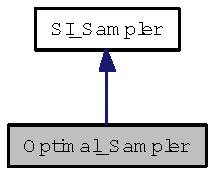
\includegraphics[width=69pt]{class_optimal___sampler__inherit__graph}
\end{center}
\end{figure}
\subsection*{Public Member Functions}
\begin{CompactItemize}
\item 
\hyperlink{class_optimal___sampler_0d07b22c5c1e33ecd586059dd5cf739e}{Optimal\_\-Sampler} (void)
\item 
\hyperlink{class_optimal___sampler_c93d1bd8e4855c1867f51b941060717b}{Optimal\_\-Sampler} (\hyperlink{class_opt___simulator}{Opt\_\-Simulator} $\ast$m)
\item 
vector$<$ \hyperlink{class_weighted___sample}{Weighted\_\-Sample} $>$ \hyperlink{class_optimal___sampler_d1f49e39bf83898c19c044a3874c6930}{DrawInitCloud} (const int \&NbSample)
\begin{CompactList}\small\item\em draw a set of possible init state \item\end{CompactList}\item 
vector$<$ \hyperlink{class_weighted___sample}{Weighted\_\-Sample} $>$ \hyperlink{class_optimal___sampler_1a9288b91deaab91d0c3d3511d6e1892}{Draw} (const dcovector \&Y\_\-k, const vector$<$ \hyperlink{class_weighted___sample}{Weighted\_\-Sample} $>$ \&X\_\-km1)
\begin{CompactList}\small\item\em Draw a set of samples from the importance density Xk given Y0:k X0:k-1. \item\end{CompactList}\item 
long double \hyperlink{class_optimal___sampler_376a6addc54dd14aee7f1367c183e100}{Weight} (vector$<$ \hyperlink{class_weighted___sample}{Weighted\_\-Sample} $>$ \&cloud, const dcovector \&Y\_\-k, const vector$<$ \hyperlink{class_weighted___sample}{Weighted\_\-Sample} $>$ \&X\_\-km1)
\begin{CompactList}\small\item\em Modify the weights of cloud for the weighting step in the sisr. \item\end{CompactList}\end{CompactItemize}


\subsection{Detailed Description}
This sampler use the optimal importance density. 



\subsection{Constructor \& Destructor Documentation}
\hypertarget{class_optimal___sampler_0d07b22c5c1e33ecd586059dd5cf739e}{
\index{Optimal\_\-Sampler@{Optimal\_\-Sampler}!Optimal\_\-Sampler@{Optimal\_\-Sampler}}
\index{Optimal\_\-Sampler@{Optimal\_\-Sampler}!Optimal_Sampler@{Optimal\_\-Sampler}}
\subsubsection[{Optimal\_\-Sampler}]{\setlength{\rightskip}{0pt plus 5cm}Optimal\_\-Sampler::Optimal\_\-Sampler (void)}}
\label{class_optimal___sampler_0d07b22c5c1e33ecd586059dd5cf739e}


\hypertarget{class_optimal___sampler_c93d1bd8e4855c1867f51b941060717b}{
\index{Optimal\_\-Sampler@{Optimal\_\-Sampler}!Optimal\_\-Sampler@{Optimal\_\-Sampler}}
\index{Optimal\_\-Sampler@{Optimal\_\-Sampler}!Optimal_Sampler@{Optimal\_\-Sampler}}
\subsubsection[{Optimal\_\-Sampler}]{\setlength{\rightskip}{0pt plus 5cm}Optimal\_\-Sampler::Optimal\_\-Sampler ({\bf Opt\_\-Simulator} $\ast$ {\em m})}}
\label{class_optimal___sampler_c93d1bd8e4855c1867f51b941060717b}




\subsection{Member Function Documentation}
\hypertarget{class_optimal___sampler_1a9288b91deaab91d0c3d3511d6e1892}{
\index{Optimal\_\-Sampler@{Optimal\_\-Sampler}!Draw@{Draw}}
\index{Draw@{Draw}!Optimal_Sampler@{Optimal\_\-Sampler}}
\subsubsection[{Draw}]{\setlength{\rightskip}{0pt plus 5cm}vector$<${\bf Weighted\_\-Sample} $>$ Optimal\_\-Sampler::Draw (const dcovector \& {\em Y\_\-k}, \/  const vector$<$ {\bf Weighted\_\-Sample} $>$ \& {\em X\_\-km1})\hspace{0.3cm}{\tt  \mbox{[}virtual\mbox{]}}}}
\label{class_optimal___sampler_1a9288b91deaab91d0c3d3511d6e1892}


Draw a set of samples from the importance density Xk given Y0:k X0:k-1. 

\begin{Desc}
\item[Parameters:]
\begin{description}
\item[{\em Y\_\-k}]The observation from 0 to k \item[{\em X\_\-km1}]The cloud from 0 to km1\end{description}
\end{Desc}
\begin{Desc}
\item[Returns:]A cloud representing the importance density q(Xk$|$Y0:k,X0:k-1) \end{Desc}


Implements \hyperlink{class_s_i___sampler_62bf57181aeb5981426a71a7bf01c3e9}{SI\_\-Sampler}.\hypertarget{class_optimal___sampler_d1f49e39bf83898c19c044a3874c6930}{
\index{Optimal\_\-Sampler@{Optimal\_\-Sampler}!DrawInitCloud@{DrawInitCloud}}
\index{DrawInitCloud@{DrawInitCloud}!Optimal_Sampler@{Optimal\_\-Sampler}}
\subsubsection[{DrawInitCloud}]{\setlength{\rightskip}{0pt plus 5cm}vector$<${\bf Weighted\_\-Sample} $>$ Optimal\_\-Sampler::DrawInitCloud (const int \& {\em NbSample})\hspace{0.3cm}{\tt  \mbox{[}virtual\mbox{]}}}}
\label{class_optimal___sampler_d1f49e39bf83898c19c044a3874c6930}


draw a set of possible init state 

\begin{Desc}
\item[Parameters:]
\begin{description}
\item[{\em NbSample}]Number of sample\end{description}
\end{Desc}
\begin{Desc}
\item[Returns:]A set of weighted samples \end{Desc}


Implements \hyperlink{class_s_i___sampler_3fbedf1ce189168da5608861d5a3289e}{SI\_\-Sampler}.\hypertarget{class_optimal___sampler_376a6addc54dd14aee7f1367c183e100}{
\index{Optimal\_\-Sampler@{Optimal\_\-Sampler}!Weight@{Weight}}
\index{Weight@{Weight}!Optimal_Sampler@{Optimal\_\-Sampler}}
\subsubsection[{Weight}]{\setlength{\rightskip}{0pt plus 5cm}long double Optimal\_\-Sampler::Weight (vector$<$ {\bf Weighted\_\-Sample} $>$ \& {\em cloud}, \/  const dcovector \& {\em Y\_\-k}, \/  const vector$<$ {\bf Weighted\_\-Sample} $>$ \& {\em X\_\-km1})\hspace{0.3cm}{\tt  \mbox{[}virtual\mbox{]}}}}
\label{class_optimal___sampler_376a6addc54dd14aee7f1367c183e100}


Modify the weights of cloud for the weighting step in the sisr. 

\begin{Desc}
\item[Parameters:]
\begin{description}
\item[{\em cloud}]The curent coud at k \item[{\em Y\_\-k}]The observation at k \item[{\em X\_\-km1}]the cloud from at km1\end{description}
\end{Desc}
\begin{Desc}
\item[Returns:]The sum of the weights \end{Desc}


Implements \hyperlink{class_s_i___sampler_5c3a3547060d91febd3ef61969756ab6}{SI\_\-Sampler}.
\hypertarget{class_opt_s_i_s_r___filter}{
\section{OptSISR\_\-Filter Class Reference}
\label{class_opt_s_i_s_r___filter}\index{OptSISR\_\-Filter@{OptSISR\_\-Filter}}
}
{\tt \#include $<$sisr\_\-filter.h$>$}

Inheritance diagram for OptSISR\_\-Filter:\nopagebreak
\begin{figure}[H]
\begin{center}
\leavevmode
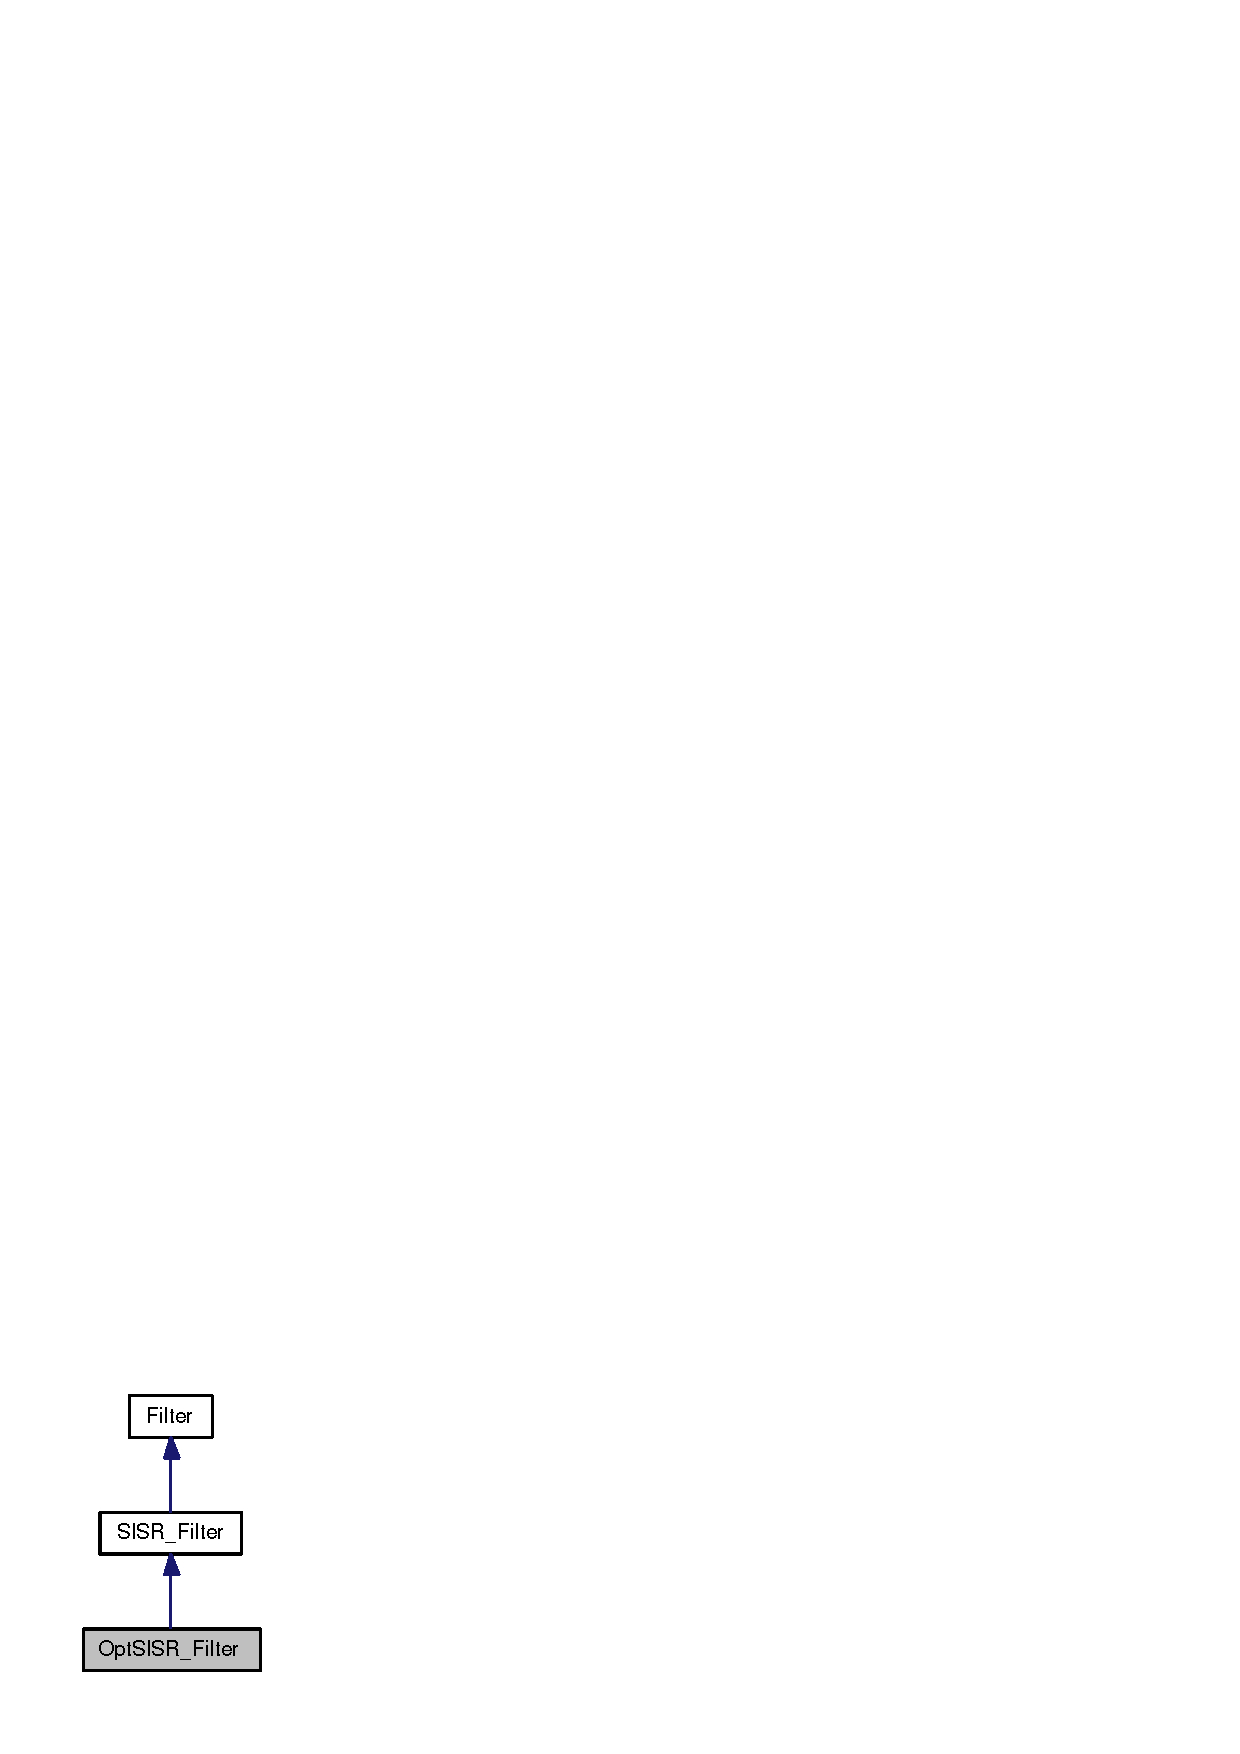
\includegraphics[width=64pt]{class_opt_s_i_s_r___filter__inherit__graph}
\end{center}
\end{figure}
\subsection*{Public Member Functions}
\begin{CompactItemize}
\item 
\hyperlink{class_opt_s_i_s_r___filter_482407cf2c2f3d45c5a6f23dbda74355}{OptSISR\_\-Filter} (void)
\item 
\hyperlink{class_opt_s_i_s_r___filter_55a22ba93049dc37183018a4078feecc}{$\sim$OptSISR\_\-Filter} (void)
\item 
\hyperlink{class_opt_s_i_s_r___filter_a9517303eb49bf062adacbbe4b6a3507}{OptSISR\_\-Filter} (const int \&Ns, \hyperlink{class_opt___simulator}{Opt\_\-Simulator} $\ast$m)
\item 
\hyperlink{class_opt_s_i_s_r___filter_3c6657eab5ca02bbe6aff027b567afa8}{OptSISR\_\-Filter} (const int \&Ns, \hyperlink{class_gaussian___nonlinear___model}{Gaussian\_\-Nonlinear\_\-Model} $\ast$m)
\end{CompactItemize}
\subsection*{Private Attributes}
\begin{CompactItemize}
\item 
\hyperlink{class_opt___simulator}{Opt\_\-Simulator} $\ast$ \hyperlink{class_opt_s_i_s_r___filter_d1eea7d9e7f91df64dd7550bf764c64f}{sim}
\end{CompactItemize}


\subsection{Constructor \& Destructor Documentation}
\hypertarget{class_opt_s_i_s_r___filter_482407cf2c2f3d45c5a6f23dbda74355}{
\index{OptSISR\_\-Filter@{OptSISR\_\-Filter}!OptSISR\_\-Filter@{OptSISR\_\-Filter}}
\index{OptSISR\_\-Filter@{OptSISR\_\-Filter}!OptSISR_Filter@{OptSISR\_\-Filter}}
\subsubsection[{OptSISR\_\-Filter}]{\setlength{\rightskip}{0pt plus 5cm}OptSISR\_\-Filter::OptSISR\_\-Filter (void)}}
\label{class_opt_s_i_s_r___filter_482407cf2c2f3d45c5a6f23dbda74355}


\hypertarget{class_opt_s_i_s_r___filter_55a22ba93049dc37183018a4078feecc}{
\index{OptSISR\_\-Filter@{OptSISR\_\-Filter}!$\sim$OptSISR\_\-Filter@{$\sim$OptSISR\_\-Filter}}
\index{$\sim$OptSISR\_\-Filter@{$\sim$OptSISR\_\-Filter}!OptSISR_Filter@{OptSISR\_\-Filter}}
\subsubsection[{$\sim$OptSISR\_\-Filter}]{\setlength{\rightskip}{0pt plus 5cm}OptSISR\_\-Filter::$\sim$OptSISR\_\-Filter (void)}}
\label{class_opt_s_i_s_r___filter_55a22ba93049dc37183018a4078feecc}


\hypertarget{class_opt_s_i_s_r___filter_a9517303eb49bf062adacbbe4b6a3507}{
\index{OptSISR\_\-Filter@{OptSISR\_\-Filter}!OptSISR\_\-Filter@{OptSISR\_\-Filter}}
\index{OptSISR\_\-Filter@{OptSISR\_\-Filter}!OptSISR_Filter@{OptSISR\_\-Filter}}
\subsubsection[{OptSISR\_\-Filter}]{\setlength{\rightskip}{0pt plus 5cm}OptSISR\_\-Filter::OptSISR\_\-Filter (const int \& {\em Ns}, \/  {\bf Opt\_\-Simulator} $\ast$ {\em m})}}
\label{class_opt_s_i_s_r___filter_a9517303eb49bf062adacbbe4b6a3507}


\hypertarget{class_opt_s_i_s_r___filter_3c6657eab5ca02bbe6aff027b567afa8}{
\index{OptSISR\_\-Filter@{OptSISR\_\-Filter}!OptSISR\_\-Filter@{OptSISR\_\-Filter}}
\index{OptSISR\_\-Filter@{OptSISR\_\-Filter}!OptSISR_Filter@{OptSISR\_\-Filter}}
\subsubsection[{OptSISR\_\-Filter}]{\setlength{\rightskip}{0pt plus 5cm}OptSISR\_\-Filter::OptSISR\_\-Filter (const int \& {\em Ns}, \/  {\bf Gaussian\_\-Nonlinear\_\-Model} $\ast$ {\em m})}}
\label{class_opt_s_i_s_r___filter_3c6657eab5ca02bbe6aff027b567afa8}




\subsection{Member Data Documentation}
\hypertarget{class_opt_s_i_s_r___filter_d1eea7d9e7f91df64dd7550bf764c64f}{
\index{OptSISR\_\-Filter@{OptSISR\_\-Filter}!sim@{sim}}
\index{sim@{sim}!OptSISR_Filter@{OptSISR\_\-Filter}}
\subsubsection[{sim}]{\setlength{\rightskip}{0pt plus 5cm}{\bf Opt\_\-Simulator}$\ast$ {\bf OptSISR\_\-Filter::sim}\hspace{0.3cm}{\tt  \mbox{[}private\mbox{]}}}}
\label{class_opt_s_i_s_r___filter_d1eea7d9e7f91df64dd7550bf764c64f}



\hypertarget{class_ozaki___c_d___model}{
\section{Ozaki\_\-CD\_\-Model Class Reference}
\label{class_ozaki___c_d___model}\index{Ozaki\_\-CD\_\-Model@{Ozaki\_\-CD\_\-Model}}
}
continuous discret model: the state SDE is discretly approximate by Ozaki method  


{\tt \#include $<$gaussian\_\-model.h$>$}

Inheritance diagram for Ozaki\_\-CD\_\-Model:\nopagebreak
\begin{figure}[H]
\begin{center}
\leavevmode
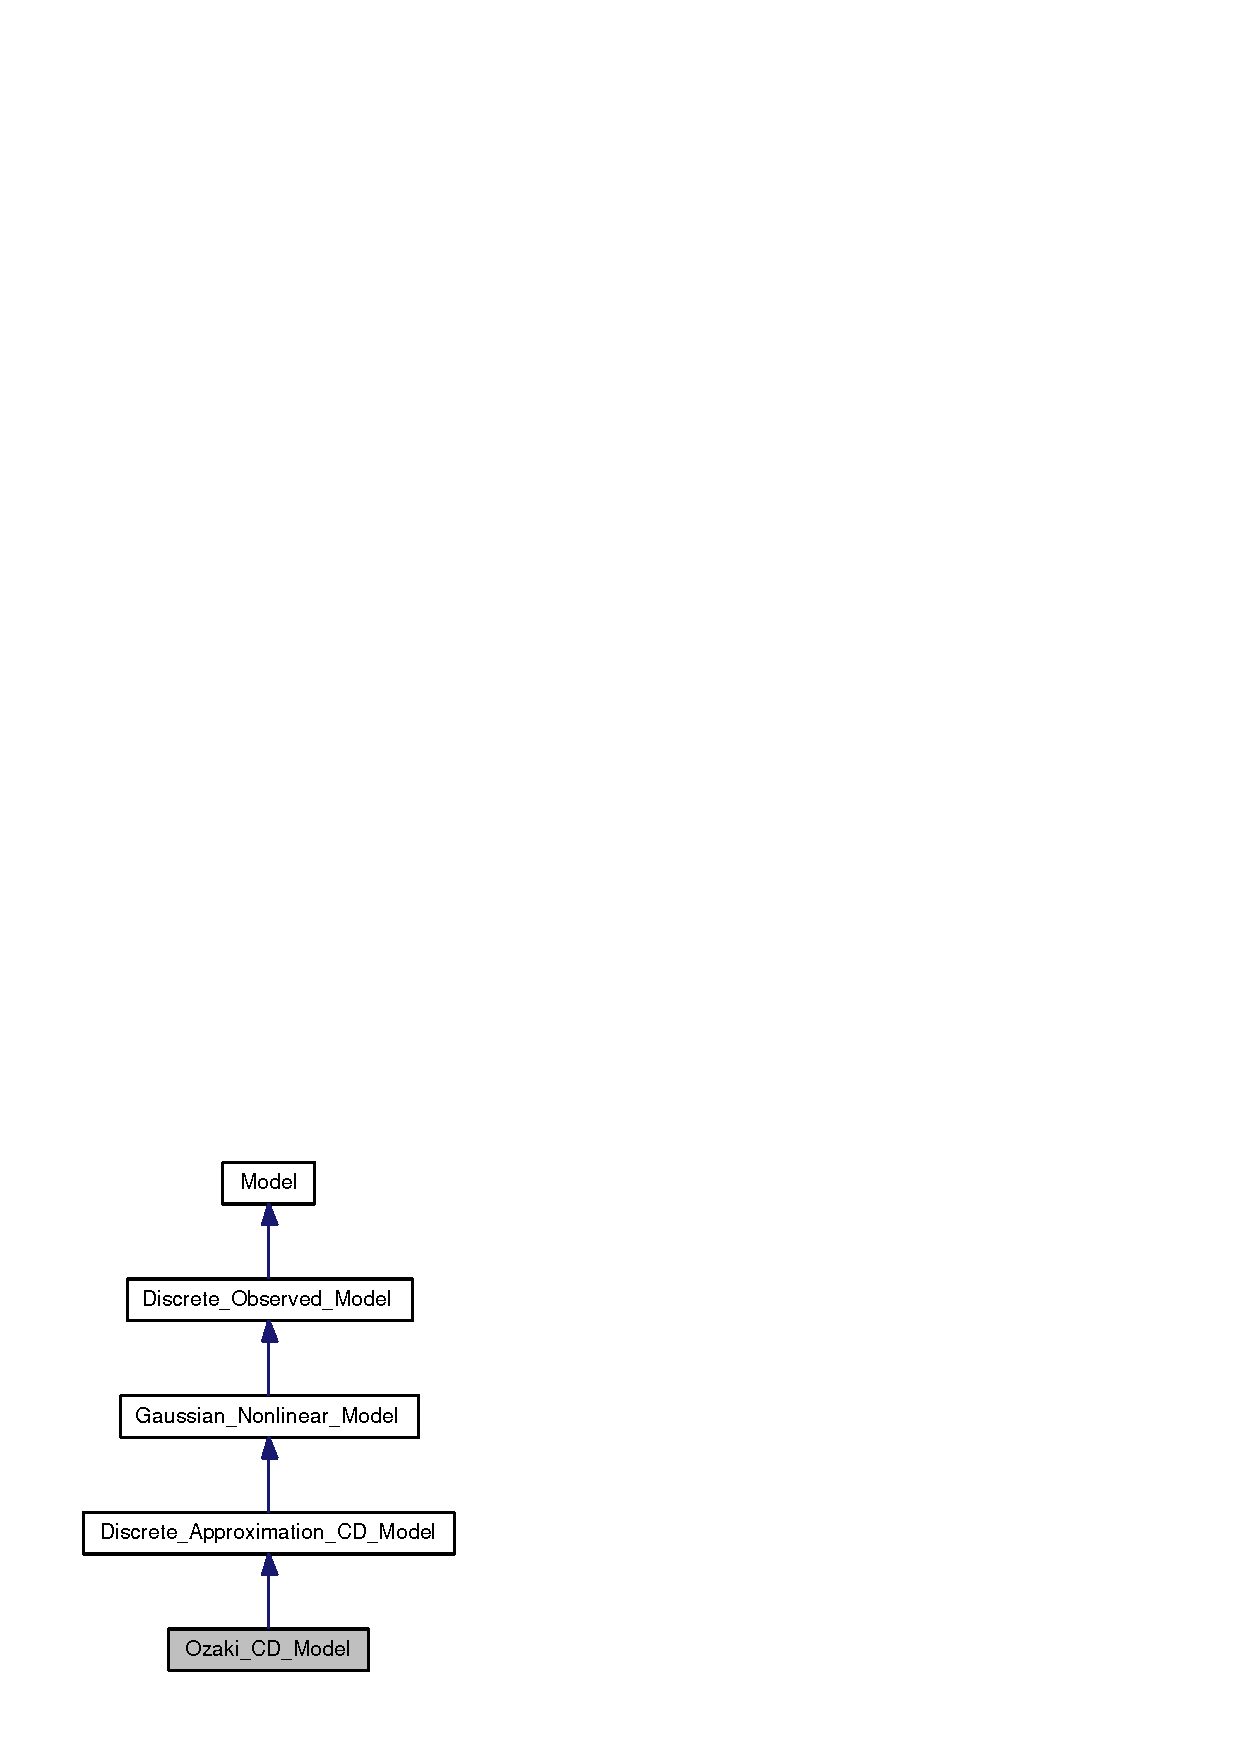
\includegraphics[width=111pt]{class_ozaki___c_d___model__inherit__graph}
\end{center}
\end{figure}
\subsection*{Public Member Functions}
\begin{CompactItemize}
\item 
\hyperlink{class_ozaki___c_d___model_97b6866d8dc6ea653b686ed224d4dc48}{Ozaki\_\-CD\_\-Model} (void)
\item 
\hyperlink{class_ozaki___c_d___model_d3a96828c7830a244327f890f8b90a65}{Ozaki\_\-CD\_\-Model} (\hyperlink{class_continuous___discrete___model}{Continuous\_\-Discrete\_\-Model} $\ast$m, const int \&a)
\item 
dcovector \hyperlink{class_ozaki___c_d___model_394a9716158c403c06c4416f01e661a9}{Scheme} (const dcovector \&X, const dcovector \&W)
\item 
dgematrix \hyperlink{class_ozaki___c_d___model_6c4415b26674d1fc7b5e4f7499f35dd9}{Jx\_\-Scheme} (const dcovector \&X, const dcovector \&W)
\item 
dgematrix \hyperlink{class_ozaki___c_d___model_66009069506580d175c869cea3df3cd6}{Jw\_\-Scheme} (const dcovector \&X, const dcovector \&W)
\item 
void \hyperlink{class_ozaki___c_d___model_c0878d9dda14cd1294e2ce7e5ab9c281}{Get\_\-Linear\_\-Scheme} (const dcovector \&X, const dcovector \&W, dgematrix \&F, dgematrix \&J, dcovector \&Xp)
\begin{CompactList}\small\item\em Get the Linearized parameters Scheme in X,W. \item\end{CompactList}\end{CompactItemize}


\subsection{Detailed Description}
continuous discret model: the state SDE is discretly approximate by Ozaki method 

\subsection{Constructor \& Destructor Documentation}
\hypertarget{class_ozaki___c_d___model_97b6866d8dc6ea653b686ed224d4dc48}{
\index{Ozaki\_\-CD\_\-Model@{Ozaki\_\-CD\_\-Model}!Ozaki\_\-CD\_\-Model@{Ozaki\_\-CD\_\-Model}}
\index{Ozaki\_\-CD\_\-Model@{Ozaki\_\-CD\_\-Model}!Ozaki_CD_Model@{Ozaki\_\-CD\_\-Model}}
\subsubsection[{Ozaki\_\-CD\_\-Model}]{\setlength{\rightskip}{0pt plus 5cm}Ozaki\_\-CD\_\-Model::Ozaki\_\-CD\_\-Model (void)}}
\label{class_ozaki___c_d___model_97b6866d8dc6ea653b686ed224d4dc48}


\hypertarget{class_ozaki___c_d___model_d3a96828c7830a244327f890f8b90a65}{
\index{Ozaki\_\-CD\_\-Model@{Ozaki\_\-CD\_\-Model}!Ozaki\_\-CD\_\-Model@{Ozaki\_\-CD\_\-Model}}
\index{Ozaki\_\-CD\_\-Model@{Ozaki\_\-CD\_\-Model}!Ozaki_CD_Model@{Ozaki\_\-CD\_\-Model}}
\subsubsection[{Ozaki\_\-CD\_\-Model}]{\setlength{\rightskip}{0pt plus 5cm}Ozaki\_\-CD\_\-Model::Ozaki\_\-CD\_\-Model ({\bf Continuous\_\-Discrete\_\-Model} $\ast$ {\em m}, \/  const int \& {\em a})}}
\label{class_ozaki___c_d___model_d3a96828c7830a244327f890f8b90a65}




\subsection{Member Function Documentation}
\hypertarget{class_ozaki___c_d___model_c0878d9dda14cd1294e2ce7e5ab9c281}{
\index{Ozaki\_\-CD\_\-Model@{Ozaki\_\-CD\_\-Model}!Get\_\-Linear\_\-Scheme@{Get\_\-Linear\_\-Scheme}}
\index{Get\_\-Linear\_\-Scheme@{Get\_\-Linear\_\-Scheme}!Ozaki_CD_Model@{Ozaki\_\-CD\_\-Model}}
\subsubsection[{Get\_\-Linear\_\-Scheme}]{\setlength{\rightskip}{0pt plus 5cm}void Ozaki\_\-CD\_\-Model::Get\_\-Linear\_\-Scheme (const dcovector \& {\em X}, \/  const dcovector \& {\em W}, \/  dgematrix \& {\em F}, \/  dgematrix \& {\em J}, \/  dcovector \& {\em Xp})\hspace{0.3cm}{\tt  \mbox{[}virtual\mbox{]}}}}
\label{class_ozaki___c_d___model_c0878d9dda14cd1294e2ce7e5ab9c281}


Get the Linearized parameters Scheme in X,W. 

\begin{Desc}
\item[Parameters:]
\begin{description}
\item[{\em X}]The state value \item[{\em W}]The noise value \item[{\em F}]The jacobian of f(X,W) in X \item[{\em G}]The jacobian in f(X,W) in W \item[{\em Xp}]The prediction Xp = f(X,W) \end{description}
\end{Desc}


Implements \hyperlink{class_discrete___approximation___c_d___model_0a486fada10e6f5569d186edc7b32110}{Discrete\_\-Approximation\_\-CD\_\-Model}.\hypertarget{class_ozaki___c_d___model_66009069506580d175c869cea3df3cd6}{
\index{Ozaki\_\-CD\_\-Model@{Ozaki\_\-CD\_\-Model}!Jw\_\-Scheme@{Jw\_\-Scheme}}
\index{Jw\_\-Scheme@{Jw\_\-Scheme}!Ozaki_CD_Model@{Ozaki\_\-CD\_\-Model}}
\subsubsection[{Jw\_\-Scheme}]{\setlength{\rightskip}{0pt plus 5cm}dgematrix Ozaki\_\-CD\_\-Model::Jw\_\-Scheme (const dcovector \& {\em X}, \/  const dcovector \& {\em W})\hspace{0.3cm}{\tt  \mbox{[}virtual\mbox{]}}}}
\label{class_ozaki___c_d___model_66009069506580d175c869cea3df3cd6}




Implements \hyperlink{class_discrete___approximation___c_d___model_c7496999409a3f05125ceb7fe85e85ab}{Discrete\_\-Approximation\_\-CD\_\-Model}.\hypertarget{class_ozaki___c_d___model_6c4415b26674d1fc7b5e4f7499f35dd9}{
\index{Ozaki\_\-CD\_\-Model@{Ozaki\_\-CD\_\-Model}!Jx\_\-Scheme@{Jx\_\-Scheme}}
\index{Jx\_\-Scheme@{Jx\_\-Scheme}!Ozaki_CD_Model@{Ozaki\_\-CD\_\-Model}}
\subsubsection[{Jx\_\-Scheme}]{\setlength{\rightskip}{0pt plus 5cm}dgematrix Ozaki\_\-CD\_\-Model::Jx\_\-Scheme (const dcovector \& {\em X}, \/  const dcovector \& {\em W})\hspace{0.3cm}{\tt  \mbox{[}virtual\mbox{]}}}}
\label{class_ozaki___c_d___model_6c4415b26674d1fc7b5e4f7499f35dd9}




Implements \hyperlink{class_discrete___approximation___c_d___model_7a3dcae055d90be0b8a231eff961e2a2}{Discrete\_\-Approximation\_\-CD\_\-Model}.\hypertarget{class_ozaki___c_d___model_394a9716158c403c06c4416f01e661a9}{
\index{Ozaki\_\-CD\_\-Model@{Ozaki\_\-CD\_\-Model}!Scheme@{Scheme}}
\index{Scheme@{Scheme}!Ozaki_CD_Model@{Ozaki\_\-CD\_\-Model}}
\subsubsection[{Scheme}]{\setlength{\rightskip}{0pt plus 5cm}dcovector Ozaki\_\-CD\_\-Model::Scheme (const dcovector \& {\em X}, \/  const dcovector \& {\em W})\hspace{0.3cm}{\tt  \mbox{[}virtual\mbox{]}}}}
\label{class_ozaki___c_d___model_394a9716158c403c06c4416f01e661a9}




Implements \hyperlink{class_discrete___approximation___c_d___model_1ea9a1d618890fc51db6fa98eeb7af7f}{Discrete\_\-Approximation\_\-CD\_\-Model}.
\hypertarget{class_s_i___sampler}{
\section{SI\_\-Sampler Class Reference}
\label{class_s_i___sampler}\index{SI\_\-Sampler@{SI\_\-Sampler}}
}
the sequential importance sampler used for sisr filter (bootstrap,optimal ...)  


{\tt \#include $<$sisr\_\-filter.h$>$}

Inheritance diagram for SI\_\-Sampler:\nopagebreak
\begin{figure}[H]
\begin{center}
\leavevmode
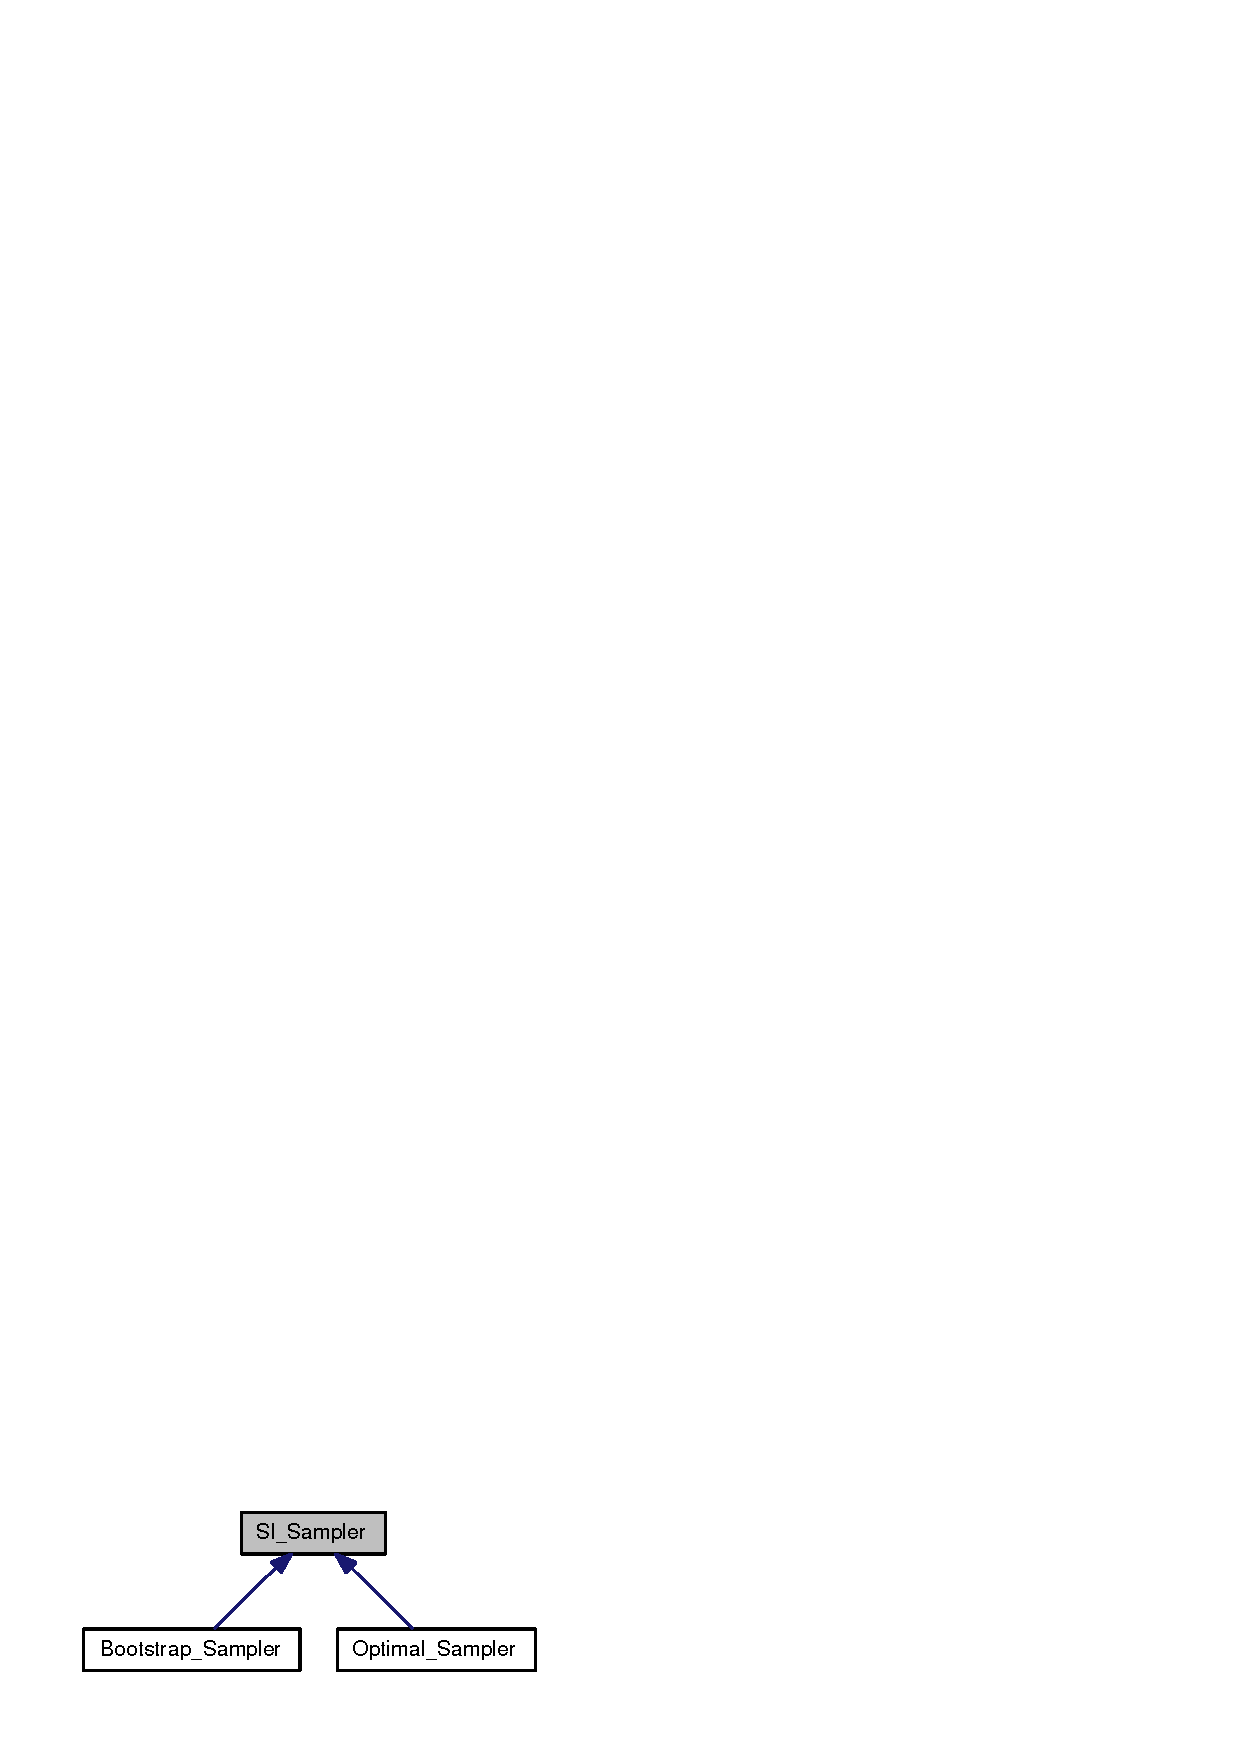
\includegraphics[width=130pt]{class_s_i___sampler__inherit__graph}
\end{center}
\end{figure}
\subsection*{Public Member Functions}
\begin{CompactItemize}
\item 
\hyperlink{class_s_i___sampler_34229c2cf9f69118ef54233deaed943e}{SI\_\-Sampler} (void)
\begin{CompactList}\small\item\em The constructor. \item\end{CompactList}\item 
\hyperlink{class_s_i___sampler_3d6f1ddcca06c4e086b4af48e0b68645}{SI\_\-Sampler} (\hyperlink{class_simulator}{Simulator} $\ast$m)
\begin{CompactList}\small\item\em constructor \item\end{CompactList}\item 
virtual vector$<$ \hyperlink{class_weighted___sample}{Weighted\_\-Sample} $>$ \hyperlink{class_s_i___sampler_3fbedf1ce189168da5608861d5a3289e}{DrawInitCloud} (const int \&NbSample)=0
\begin{CompactList}\small\item\em draw a set of possible init state \item\end{CompactList}\item 
virtual vector$<$ \hyperlink{class_weighted___sample}{Weighted\_\-Sample} $>$ \hyperlink{class_s_i___sampler_62bf57181aeb5981426a71a7bf01c3e9}{Draw} (const dcovector \&Y\_\-k, const vector$<$ \hyperlink{class_weighted___sample}{Weighted\_\-Sample} $>$ \&X\_\-km1)=0
\begin{CompactList}\small\item\em Draw a set of samples from the importance density Xk given Y0:k X0:k-1. \item\end{CompactList}\item 
virtual long double \hyperlink{class_s_i___sampler_5c3a3547060d91febd3ef61969756ab6}{Weight} (vector$<$ \hyperlink{class_weighted___sample}{Weighted\_\-Sample} $>$ \&cloud, const dcovector \&Y\_\-k, const vector$<$ \hyperlink{class_weighted___sample}{Weighted\_\-Sample} $>$ \&X\_\-km1)=0
\begin{CompactList}\small\item\em Modify the weights of cloud for the weighting step in the sisr. \item\end{CompactList}\end{CompactItemize}
\subsection*{Public Attributes}
\begin{CompactItemize}
\item 
\hyperlink{class_simulator}{Simulator} $\ast$ \hyperlink{class_s_i___sampler_b79ecd357866d7ed5ab1867c4a5633e7}{model}
\end{CompactItemize}


\subsection{Detailed Description}
the sequential importance sampler used for sisr filter (bootstrap,optimal ...) 



\subsection{Constructor \& Destructor Documentation}
\hypertarget{class_s_i___sampler_34229c2cf9f69118ef54233deaed943e}{
\index{SI\_\-Sampler@{SI\_\-Sampler}!SI\_\-Sampler@{SI\_\-Sampler}}
\index{SI\_\-Sampler@{SI\_\-Sampler}!SI_Sampler@{SI\_\-Sampler}}
\subsubsection[{SI\_\-Sampler}]{\setlength{\rightskip}{0pt plus 5cm}SI\_\-Sampler::SI\_\-Sampler (void)}}
\label{class_s_i___sampler_34229c2cf9f69118ef54233deaed943e}


The constructor. 

\hypertarget{class_s_i___sampler_3d6f1ddcca06c4e086b4af48e0b68645}{
\index{SI\_\-Sampler@{SI\_\-Sampler}!SI\_\-Sampler@{SI\_\-Sampler}}
\index{SI\_\-Sampler@{SI\_\-Sampler}!SI_Sampler@{SI\_\-Sampler}}
\subsubsection[{SI\_\-Sampler}]{\setlength{\rightskip}{0pt plus 5cm}SI\_\-Sampler::SI\_\-Sampler ({\bf Simulator} $\ast$ {\em m})}}
\label{class_s_i___sampler_3d6f1ddcca06c4e086b4af48e0b68645}


constructor 

The constructor \begin{Desc}
\item[Parameters:]
\begin{description}
\item[{\em m}]A discrete model \end{description}
\end{Desc}


\subsection{Member Function Documentation}
\hypertarget{class_s_i___sampler_62bf57181aeb5981426a71a7bf01c3e9}{
\index{SI\_\-Sampler@{SI\_\-Sampler}!Draw@{Draw}}
\index{Draw@{Draw}!SI_Sampler@{SI\_\-Sampler}}
\subsubsection[{Draw}]{\setlength{\rightskip}{0pt plus 5cm}virtual vector$<${\bf Weighted\_\-Sample} $>$ SI\_\-Sampler::Draw (const dcovector \& {\em Y\_\-k}, \/  const vector$<$ {\bf Weighted\_\-Sample} $>$ \& {\em X\_\-km1})\hspace{0.3cm}{\tt  \mbox{[}pure virtual\mbox{]}}}}
\label{class_s_i___sampler_62bf57181aeb5981426a71a7bf01c3e9}


Draw a set of samples from the importance density Xk given Y0:k X0:k-1. 

\begin{Desc}
\item[Parameters:]
\begin{description}
\item[{\em Y\_\-k}]The observation from 0 to k \item[{\em X\_\-km1}]The cloud from 0 to km1\end{description}
\end{Desc}
\begin{Desc}
\item[Returns:]A cloud representing the importance density q(Xk$|$Y0:k,X0:k-1) \end{Desc}


Implemented in \hyperlink{class_bootstrap___sampler_a826164a46c257f5a95ba0b4eba7ee83}{Bootstrap\_\-Sampler}, and \hyperlink{class_optimal___sampler_1a9288b91deaab91d0c3d3511d6e1892}{Optimal\_\-Sampler}.\hypertarget{class_s_i___sampler_3fbedf1ce189168da5608861d5a3289e}{
\index{SI\_\-Sampler@{SI\_\-Sampler}!DrawInitCloud@{DrawInitCloud}}
\index{DrawInitCloud@{DrawInitCloud}!SI_Sampler@{SI\_\-Sampler}}
\subsubsection[{DrawInitCloud}]{\setlength{\rightskip}{0pt plus 5cm}virtual vector$<${\bf Weighted\_\-Sample} $>$ SI\_\-Sampler::DrawInitCloud (const int \& {\em NbSample})\hspace{0.3cm}{\tt  \mbox{[}pure virtual\mbox{]}}}}
\label{class_s_i___sampler_3fbedf1ce189168da5608861d5a3289e}


draw a set of possible init state 

\begin{Desc}
\item[Parameters:]
\begin{description}
\item[{\em NbSample}]Number of sample\end{description}
\end{Desc}
\begin{Desc}
\item[Returns:]A set of weighted samples \end{Desc}


Implemented in \hyperlink{class_bootstrap___sampler_e36eb9258b052c41e075b350960d21a3}{Bootstrap\_\-Sampler}, and \hyperlink{class_optimal___sampler_d1f49e39bf83898c19c044a3874c6930}{Optimal\_\-Sampler}.\hypertarget{class_s_i___sampler_5c3a3547060d91febd3ef61969756ab6}{
\index{SI\_\-Sampler@{SI\_\-Sampler}!Weight@{Weight}}
\index{Weight@{Weight}!SI_Sampler@{SI\_\-Sampler}}
\subsubsection[{Weight}]{\setlength{\rightskip}{0pt plus 5cm}virtual long double SI\_\-Sampler::Weight (vector$<$ {\bf Weighted\_\-Sample} $>$ \& {\em cloud}, \/  const dcovector \& {\em Y\_\-k}, \/  const vector$<$ {\bf Weighted\_\-Sample} $>$ \& {\em X\_\-km1})\hspace{0.3cm}{\tt  \mbox{[}pure virtual\mbox{]}}}}
\label{class_s_i___sampler_5c3a3547060d91febd3ef61969756ab6}


Modify the weights of cloud for the weighting step in the sisr. 

\begin{Desc}
\item[Parameters:]
\begin{description}
\item[{\em cloud}]The curent coud at k \item[{\em Y\_\-k}]The observation at k \item[{\em X\_\-km1}]the cloud from at km1\end{description}
\end{Desc}
\begin{Desc}
\item[Returns:]The sum of the weights \end{Desc}


Implemented in \hyperlink{class_bootstrap___sampler_22ca201b958c0c873cfdbd1d545140dc}{Bootstrap\_\-Sampler}, and \hyperlink{class_optimal___sampler_376a6addc54dd14aee7f1367c183e100}{Optimal\_\-Sampler}.

\subsection{Member Data Documentation}
\hypertarget{class_s_i___sampler_b79ecd357866d7ed5ab1867c4a5633e7}{
\index{SI\_\-Sampler@{SI\_\-Sampler}!model@{model}}
\index{model@{model}!SI_Sampler@{SI\_\-Sampler}}
\subsubsection[{model}]{\setlength{\rightskip}{0pt plus 5cm}{\bf Simulator}$\ast$ {\bf SI\_\-Sampler::model}}}
\label{class_s_i___sampler_b79ecd357866d7ed5ab1867c4a5633e7}



\hypertarget{class_simulator}{
\section{Simulator Class Reference}
\label{class_simulator}\index{Simulator@{Simulator}}
}
{\tt \#include $<$simulator.h$>$}

Inheritance diagram for Simulator:\nopagebreak
\begin{figure}[H]
\begin{center}
\leavevmode
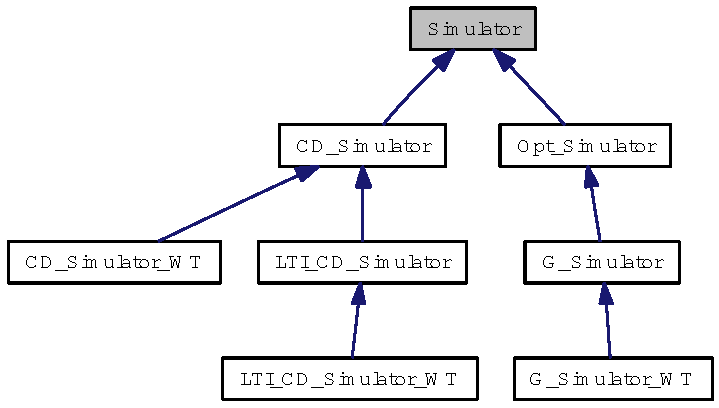
\includegraphics[width=190pt]{class_simulator__inherit__graph}
\end{center}
\end{figure}
\subsection*{Public Member Functions}
\begin{CompactItemize}
\item 
\hyperlink{class_simulator_62ab66763cb9e6cccbe88d45ab55547f}{Simulator} (void)
\item 
\hyperlink{class_simulator_39483d076c375dcf4cb826d828abd530}{$\sim$Simulator} (void)
\item 
void \hyperlink{class_simulator_e754c135109204307e1fe08f13d8bcf6}{Set\_\-Seed} (const int \&s)
\item 
virtual dcovector \hyperlink{class_simulator_29b9603eb2be9139972816329e8663dc}{Draw\_\-Init} (void)=0
\begin{CompactList}\small\item\em Draw a sample from p(X0). \item\end{CompactList}\item 
virtual dcovector \hyperlink{class_simulator_45790421a1c2f597739d3e972ad28292}{Draw\_\-Transition} (const dcovector \&Xkm1)=0
\begin{CompactList}\small\item\em Draw a sample from the transition densisty p(Xk$|$Xk-1). \item\end{CompactList}\item 
virtual dcovector \hyperlink{class_simulator_2fb966c2c2a4c93bb6788e15563c9006}{Draw\_\-Observation} (const dcovector \&Xk)=0
\begin{CompactList}\small\item\em Calculate the value of the density of probability of Y given X : p(Y$|$X). \item\end{CompactList}\item 
virtual long double \hyperlink{class_simulator_75b0dfb5b0b88346ecb9f7da4fbd91f1}{Observation\_\-Density} (const dcovector \&\hyperlink{class_simulator_403a127c909abf3e4c6d48a287315987}{Y}, const dcovector \&\hyperlink{class_simulator_a2db8ace19099d996be516022d230bc0}{X})=0
\begin{CompactList}\small\item\em calculate the value of the density of probability of Y given X : p(Y$|$X) \item\end{CompactList}\item 
virtual void \hyperlink{class_simulator_72b85e07dd0f69c4efac9178fbd2760a}{Simulate} (const int \&N)
\begin{CompactList}\small\item\em simulate the markovian model \item\end{CompactList}\item 
virtual void \hyperlink{class_simulator_7d25eafb65a104053c4fcb676ca71d1f}{Update} (void)
\begin{CompactList}\small\item\em Update the simulation of the markovian model. \item\end{CompactList}\item 
virtual int \hyperlink{class_simulator_47da05750f6f78051dcdecb5da666653}{Save\_\-X} (const char $\ast$filename)
\begin{CompactList}\small\item\em Save the simulated state trajectory in filename. \item\end{CompactList}\item 
virtual int \hyperlink{class_simulator_2cc53f33162bf08a6ae187ad4d34fe6e}{Save\_\-Y} (const char $\ast$filename)
\begin{CompactList}\small\item\em Save the simulated observation trajectory in filename. \item\end{CompactList}\item 
void \hyperlink{class_simulator_7f2f4f851a59b2e566692926c3a87940}{Clear} (void)
\begin{CompactList}\small\item\em Clear the simulated trajectory X and Y. \item\end{CompactList}\end{CompactItemize}
\subsection*{Public Attributes}
\begin{CompactItemize}
\item 
\hyperlink{class_model}{Model} $\ast$ \hyperlink{class_simulator_ab8f86e4e70af8f5a1a6c885e03d9bed}{model}
\item 
vector$<$ dcovector $>$ \hyperlink{class_simulator_a2db8ace19099d996be516022d230bc0}{X}
\item 
vector$<$ dcovector $>$ \hyperlink{class_simulator_403a127c909abf3e4c6d48a287315987}{Y}
\item 
dcovector($\ast$ \hyperlink{class_simulator_b5b842f75497c70ddb2edcaa5f731506}{b} )(void $\ast$p, gsl\_\-rng $\ast$rng)
\begin{CompactList}\small\item\em A pointer for stochastic input. \item\end{CompactList}\end{CompactItemize}
\subsection*{Protected Member Functions}
\begin{CompactItemize}
\item 
virtual void \hyperlink{class_simulator_d4aa197c02a87ff2653b54c0b9207a33}{\_\-update} (void)
\end{CompactItemize}
\subsection*{Protected Attributes}
\begin{CompactItemize}
\item 
gsl\_\-rng $\ast$ \hyperlink{class_simulator_9e44f21a53c12fb2da041531c41dae8e}{r}
\end{CompactItemize}


\subsection{Constructor \& Destructor Documentation}
\hypertarget{class_simulator_62ab66763cb9e6cccbe88d45ab55547f}{
\index{Simulator@{Simulator}!Simulator@{Simulator}}
\index{Simulator@{Simulator}!Simulator@{Simulator}}
\subsubsection[{Simulator}]{\setlength{\rightskip}{0pt plus 5cm}Simulator::Simulator (void)}}
\label{class_simulator_62ab66763cb9e6cccbe88d45ab55547f}


\hypertarget{class_simulator_39483d076c375dcf4cb826d828abd530}{
\index{Simulator@{Simulator}!$\sim$Simulator@{$\sim$Simulator}}
\index{$\sim$Simulator@{$\sim$Simulator}!Simulator@{Simulator}}
\subsubsection[{$\sim$Simulator}]{\setlength{\rightskip}{0pt plus 5cm}Simulator::$\sim$Simulator (void)}}
\label{class_simulator_39483d076c375dcf4cb826d828abd530}




\subsection{Member Function Documentation}
\hypertarget{class_simulator_d4aa197c02a87ff2653b54c0b9207a33}{
\index{Simulator@{Simulator}!\_\-update@{\_\-update}}
\index{\_\-update@{\_\-update}!Simulator@{Simulator}}
\subsubsection[{\_\-update}]{\setlength{\rightskip}{0pt plus 5cm}virtual void Simulator::\_\-update (void)\hspace{0.3cm}{\tt  \mbox{[}protected, virtual\mbox{]}}}}
\label{class_simulator_d4aa197c02a87ff2653b54c0b9207a33}




Reimplemented in \hyperlink{class_c_d___simulator_efc4b4521a9d4cd6658c16feb9233e14}{CD\_\-Simulator}.\hypertarget{class_simulator_7f2f4f851a59b2e566692926c3a87940}{
\index{Simulator@{Simulator}!Clear@{Clear}}
\index{Clear@{Clear}!Simulator@{Simulator}}
\subsubsection[{Clear}]{\setlength{\rightskip}{0pt plus 5cm}void Simulator::Clear (void)}}
\label{class_simulator_7f2f4f851a59b2e566692926c3a87940}


Clear the simulated trajectory X and Y. 

\hypertarget{class_simulator_29b9603eb2be9139972816329e8663dc}{
\index{Simulator@{Simulator}!Draw\_\-Init@{Draw\_\-Init}}
\index{Draw\_\-Init@{Draw\_\-Init}!Simulator@{Simulator}}
\subsubsection[{Draw\_\-Init}]{\setlength{\rightskip}{0pt plus 5cm}virtual dcovector Simulator::Draw\_\-Init (void)\hspace{0.3cm}{\tt  \mbox{[}pure virtual\mbox{]}}}}
\label{class_simulator_29b9603eb2be9139972816329e8663dc}


Draw a sample from p(X0). 

\begin{Desc}
\item[Returns:]A sample from p(X0) \end{Desc}


Implemented in \hyperlink{class_g___simulator_0e9a1d220c5457cc07c6bcdb70e1638c}{G\_\-Simulator}, \hyperlink{class_g___simulator___w_t_4dab061e25ad9b7b6c279d65ea3038d2}{G\_\-Simulator\_\-WT}, \hyperlink{class_c_d___simulator_cbdbea3e487026be0c032d2218d27b2b}{CD\_\-Simulator}, \hyperlink{class_c_d___simulator___w_t_c05069bbef8e4ff83247f77476b2afe1}{CD\_\-Simulator\_\-WT}, and \hyperlink{class_l_t_i___c_d___simulator___w_t_a63eaac608a5f214468dc13d34f8f20f}{LTI\_\-CD\_\-Simulator\_\-WT}.\hypertarget{class_simulator_2fb966c2c2a4c93bb6788e15563c9006}{
\index{Simulator@{Simulator}!Draw\_\-Observation@{Draw\_\-Observation}}
\index{Draw\_\-Observation@{Draw\_\-Observation}!Simulator@{Simulator}}
\subsubsection[{Draw\_\-Observation}]{\setlength{\rightskip}{0pt plus 5cm}virtual dcovector Simulator::Draw\_\-Observation (const dcovector \& {\em Xk})\hspace{0.3cm}{\tt  \mbox{[}pure virtual\mbox{]}}}}
\label{class_simulator_2fb966c2c2a4c93bb6788e15563c9006}


Calculate the value of the density of probability of Y given X : p(Y$|$X). 

\begin{Desc}
\item[Parameters:]
\begin{description}
\item[{\em Xk}]The state at k\end{description}
\end{Desc}
\begin{Desc}
\item[Returns:]The simulated observation \end{Desc}


Implemented in \hyperlink{class_g___simulator_b53bc573683cef16a5117dcc71a1f0a7}{G\_\-Simulator}, and \hyperlink{class_c_d___simulator_3770eddf939898b6dccc39a556eaf8c9}{CD\_\-Simulator}.\hypertarget{class_simulator_45790421a1c2f597739d3e972ad28292}{
\index{Simulator@{Simulator}!Draw\_\-Transition@{Draw\_\-Transition}}
\index{Draw\_\-Transition@{Draw\_\-Transition}!Simulator@{Simulator}}
\subsubsection[{Draw\_\-Transition}]{\setlength{\rightskip}{0pt plus 5cm}virtual dcovector Simulator::Draw\_\-Transition (const dcovector \& {\em Xkm1})\hspace{0.3cm}{\tt  \mbox{[}pure virtual\mbox{]}}}}
\label{class_simulator_45790421a1c2f597739d3e972ad28292}


Draw a sample from the transition densisty p(Xk$|$Xk-1). 

\begin{Desc}
\item[Parameters:]
\begin{description}
\item[{\em Xkm1}]X(k-1) the preceding state\end{description}
\end{Desc}
\begin{Desc}
\item[Returns:]\end{Desc}


Implemented in \hyperlink{class_g___simulator_54563826e17b08d4cf66090731797888}{G\_\-Simulator}, and \hyperlink{class_c_d___simulator_58019a5001ec77da3233b072f6328b30}{CD\_\-Simulator}.\hypertarget{class_simulator_75b0dfb5b0b88346ecb9f7da4fbd91f1}{
\index{Simulator@{Simulator}!Observation\_\-Density@{Observation\_\-Density}}
\index{Observation\_\-Density@{Observation\_\-Density}!Simulator@{Simulator}}
\subsubsection[{Observation\_\-Density}]{\setlength{\rightskip}{0pt plus 5cm}virtual long double Simulator::Observation\_\-Density (const dcovector \& {\em Y}, \/  const dcovector \& {\em X})\hspace{0.3cm}{\tt  \mbox{[}pure virtual\mbox{]}}}}
\label{class_simulator_75b0dfb5b0b88346ecb9f7da4fbd91f1}


calculate the value of the density of probability of Y given X : p(Y$|$X) 

\begin{Desc}
\item[Parameters:]
\begin{description}
\item[{\em Y}]The osbervation \item[{\em X}]The state\end{description}
\end{Desc}
\begin{Desc}
\item[Returns:]The value of the density \end{Desc}


Implemented in \hyperlink{class_g___simulator_6f42783322c20a0b91fab9f1e6d54363}{G\_\-Simulator}, and \hyperlink{class_c_d___simulator_905fb2ac4a72f5d7e44957fa8103cab8}{CD\_\-Simulator}.\hypertarget{class_simulator_47da05750f6f78051dcdecb5da666653}{
\index{Simulator@{Simulator}!Save\_\-X@{Save\_\-X}}
\index{Save\_\-X@{Save\_\-X}!Simulator@{Simulator}}
\subsubsection[{Save\_\-X}]{\setlength{\rightskip}{0pt plus 5cm}virtual int Simulator::Save\_\-X (const char $\ast$ {\em filename})\hspace{0.3cm}{\tt  \mbox{[}virtual\mbox{]}}}}
\label{class_simulator_47da05750f6f78051dcdecb5da666653}


Save the simulated state trajectory in filename. 

\begin{Desc}
\item[Parameters:]
\begin{description}
\item[{\em filename}]The file\end{description}
\end{Desc}
\begin{Desc}
\item[Returns:]0 if it's ok \end{Desc}


Reimplemented in \hyperlink{class_c_d___simulator_7d9d7bb805654ee7ee1f2235364bc19e}{CD\_\-Simulator}.\hypertarget{class_simulator_2cc53f33162bf08a6ae187ad4d34fe6e}{
\index{Simulator@{Simulator}!Save\_\-Y@{Save\_\-Y}}
\index{Save\_\-Y@{Save\_\-Y}!Simulator@{Simulator}}
\subsubsection[{Save\_\-Y}]{\setlength{\rightskip}{0pt plus 5cm}virtual int Simulator::Save\_\-Y (const char $\ast$ {\em filename})\hspace{0.3cm}{\tt  \mbox{[}virtual\mbox{]}}}}
\label{class_simulator_2cc53f33162bf08a6ae187ad4d34fe6e}


Save the simulated observation trajectory in filename. 

\begin{Desc}
\item[Parameters:]
\begin{description}
\item[{\em filename}]The file\end{description}
\end{Desc}
\begin{Desc}
\item[Returns:]0 if it's ok \end{Desc}


Reimplemented in \hyperlink{class_c_d___simulator_f9d3fb4fbc4b77afd81fb8b67e003cee}{CD\_\-Simulator}.\hypertarget{class_simulator_e754c135109204307e1fe08f13d8bcf6}{
\index{Simulator@{Simulator}!Set\_\-Seed@{Set\_\-Seed}}
\index{Set\_\-Seed@{Set\_\-Seed}!Simulator@{Simulator}}
\subsubsection[{Set\_\-Seed}]{\setlength{\rightskip}{0pt plus 5cm}void Simulator::Set\_\-Seed (const int \& {\em s})}}
\label{class_simulator_e754c135109204307e1fe08f13d8bcf6}


\hypertarget{class_simulator_72b85e07dd0f69c4efac9178fbd2760a}{
\index{Simulator@{Simulator}!Simulate@{Simulate}}
\index{Simulate@{Simulate}!Simulator@{Simulator}}
\subsubsection[{Simulate}]{\setlength{\rightskip}{0pt plus 5cm}virtual void Simulator::Simulate (const int \& {\em N})\hspace{0.3cm}{\tt  \mbox{[}virtual\mbox{]}}}}
\label{class_simulator_72b85e07dd0f69c4efac9178fbd2760a}


simulate the markovian model 

\begin{Desc}
\item[Parameters:]
\begin{description}
\item[{\em N}]The duration \item[{\em X}]The state trajectory \item[{\em Y}]The output \end{description}
\end{Desc}
\hypertarget{class_simulator_7d25eafb65a104053c4fcb676ca71d1f}{
\index{Simulator@{Simulator}!Update@{Update}}
\index{Update@{Update}!Simulator@{Simulator}}
\subsubsection[{Update}]{\setlength{\rightskip}{0pt plus 5cm}virtual void Simulator::Update (void)\hspace{0.3cm}{\tt  \mbox{[}virtual\mbox{]}}}}
\label{class_simulator_7d25eafb65a104053c4fcb676ca71d1f}


Update the simulation of the markovian model. 

\begin{Desc}
\item[Parameters:]
\begin{description}
\item[{\em N}]The duration \item[{\em X}]The state trajectory \item[{\em Y}]The output \end{description}
\end{Desc}


\subsection{Member Data Documentation}
\hypertarget{class_simulator_b5b842f75497c70ddb2edcaa5f731506}{
\index{Simulator@{Simulator}!b@{b}}
\index{b@{b}!Simulator@{Simulator}}
\subsubsection[{b}]{\setlength{\rightskip}{0pt plus 5cm}dcovector($\ast$ {\bf Simulator::b})(void $\ast$p, gsl\_\-rng $\ast$rng)}}
\label{class_simulator_b5b842f75497c70ddb2edcaa5f731506}


A pointer for stochastic input. 

\hypertarget{class_simulator_ab8f86e4e70af8f5a1a6c885e03d9bed}{
\index{Simulator@{Simulator}!model@{model}}
\index{model@{model}!Simulator@{Simulator}}
\subsubsection[{model}]{\setlength{\rightskip}{0pt plus 5cm}{\bf Model}$\ast$ {\bf Simulator::model}}}
\label{class_simulator_ab8f86e4e70af8f5a1a6c885e03d9bed}


\hypertarget{class_simulator_9e44f21a53c12fb2da041531c41dae8e}{
\index{Simulator@{Simulator}!r@{r}}
\index{r@{r}!Simulator@{Simulator}}
\subsubsection[{r}]{\setlength{\rightskip}{0pt plus 5cm}gsl\_\-rng$\ast$ {\bf Simulator::r}\hspace{0.3cm}{\tt  \mbox{[}protected\mbox{]}}}}
\label{class_simulator_9e44f21a53c12fb2da041531c41dae8e}


\hypertarget{class_simulator_a2db8ace19099d996be516022d230bc0}{
\index{Simulator@{Simulator}!X@{X}}
\index{X@{X}!Simulator@{Simulator}}
\subsubsection[{X}]{\setlength{\rightskip}{0pt plus 5cm}vector$<$dcovector$>$ {\bf Simulator::X}}}
\label{class_simulator_a2db8ace19099d996be516022d230bc0}


\hypertarget{class_simulator_403a127c909abf3e4c6d48a287315987}{
\index{Simulator@{Simulator}!Y@{Y}}
\index{Y@{Y}!Simulator@{Simulator}}
\subsubsection[{Y}]{\setlength{\rightskip}{0pt plus 5cm}vector$<$dcovector$>$ {\bf Simulator::Y}}}
\label{class_simulator_403a127c909abf3e4c6d48a287315987}



\hypertarget{class_s_i_s_r___filter}{
\section{SISR\_\-Filter Class Reference}
\label{class_s_i_s_r___filter}\index{SISR\_\-Filter@{SISR\_\-Filter}}
}
{\tt \#include $<$sisr\_\-filter.h$>$}

Inheritance diagram for SISR\_\-Filter:\nopagebreak
\begin{figure}[H]
\begin{center}
\leavevmode
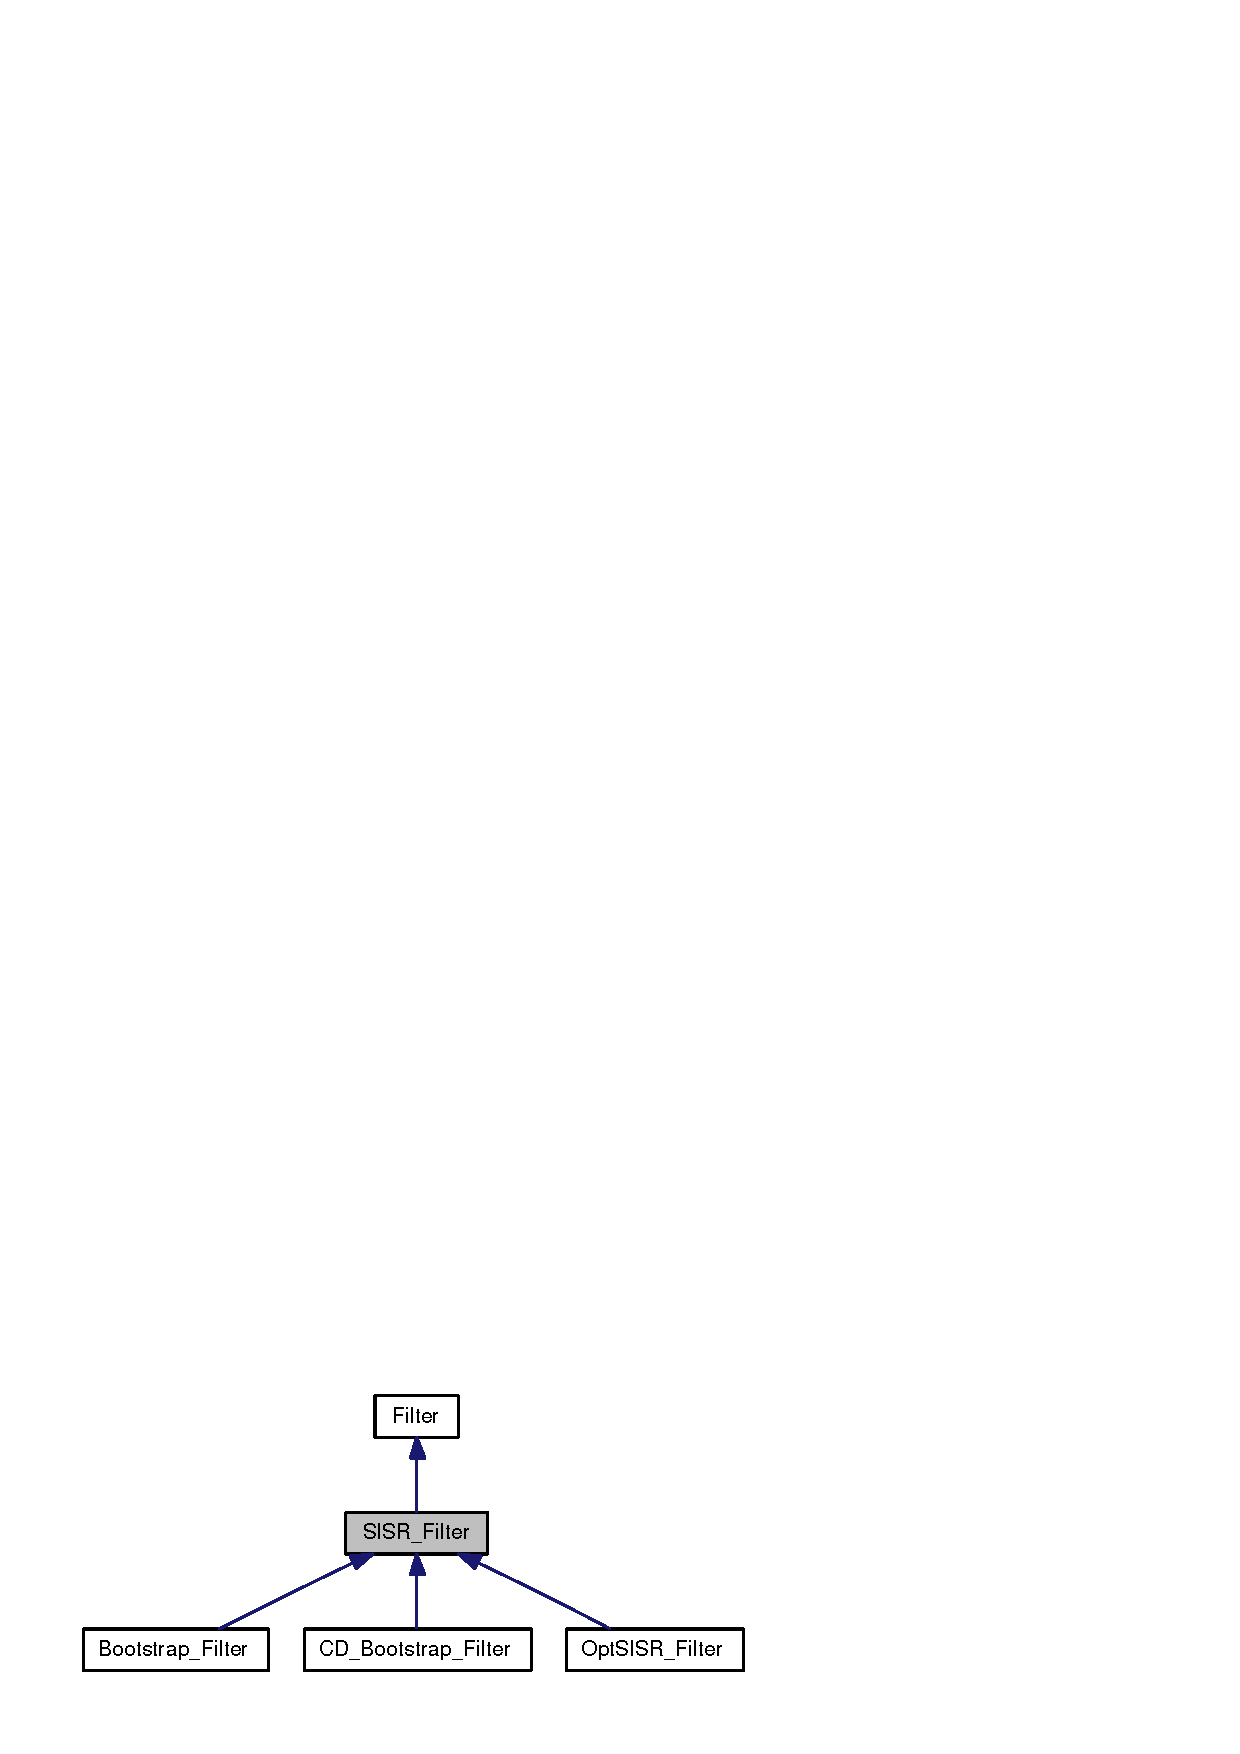
\includegraphics[width=180pt]{class_s_i_s_r___filter__inherit__graph}
\end{center}
\end{figure}
\subsection*{Public Member Functions}
\begin{CompactItemize}
\item 
\hyperlink{class_s_i_s_r___filter_ea2d9da796f3b59061d3c20b8d260794}{SISR\_\-Filter} (void)
\begin{CompactList}\small\item\em A constructor. \item\end{CompactList}\item 
\hyperlink{class_s_i_s_r___filter_9b76e88c5ce33eb3f3835084feaffb8c}{$\sim$SISR\_\-Filter} (void)
\begin{CompactList}\small\item\em The destructor. \item\end{CompactList}\item 
\hyperlink{class_s_i_s_r___filter_ee8aaf7607b94e836bf5a8227b741e83}{SISR\_\-Filter} (const int \&Ns, \hyperlink{class_s_i___sampler}{SI\_\-Sampler} $\ast$s)
\begin{CompactList}\small\item\em A constructor. \item\end{CompactList}\item 
\hyperlink{class_s_i_s_r___filter_ac330d4b6001a394af4beb4ee46b1909}{SISR\_\-Filter} (const int \&Ns, const double \&rc, const int \&\hyperlink{class_s_i_s_r___filter_aefe1be49175842bd0bd115e0f2dd647}{seed}, \hyperlink{class_s_i___sampler}{SI\_\-Sampler} $\ast$s)
\begin{CompactList}\small\item\em A constructor. \item\end{CompactList}\item 
void \hyperlink{class_s_i_s_r___filter_5044fef30828c3303ad1dbc83cadcc06}{SetSeed} (const int \&s)
\begin{CompactList}\small\item\em Set the seed of the random number generator of the discret pdf. \item\end{CompactList}\item 
void \hyperlink{class_s_i_s_r___filter_615f0daa6560454c0d2190020a5bb06c}{Resampling} (const int \&Ns)
\begin{CompactList}\small\item\em The resampling step. \item\end{CompactList}\item 
vector$<$ \hyperlink{class_weighted___sample}{Weighted\_\-Sample} $>$ \hyperlink{class_s_i_s_r___filter_9ee7212b795b51f2c13e06d84bebe9cb}{CloudGet} (void)
\begin{CompactList}\small\item\em get The current cloud \item\end{CompactList}\item 
void \hyperlink{class_s_i_s_r___filter_08cb01476a0433a7414fe4e4be82d572}{SetRc} (const float \&rc)
\item 
dcovector \hyperlink{class_s_i_s_r___filter_2d1eb0ceb62531ed48af9a424bc62210}{Expected\_\-Get} (void)
\end{CompactItemize}
\subsection*{Public Attributes}
\begin{CompactItemize}
\item 
vector$<$ \hyperlink{class_weighted___sample}{Weighted\_\-Sample} $>$ \hyperlink{class_s_i_s_r___filter_abf9ea165b2caafbe8b0ed1f4182419e}{cloud\_\-km1}
\begin{CompactList}\small\item\em The particle clouds at km1. \item\end{CompactList}\item 
vector$<$ \hyperlink{class_weighted___sample}{Weighted\_\-Sample} $>$ \hyperlink{class_s_i_s_r___filter_7ac75002d39baceda7ef98f1551243bd}{cloud}
\begin{CompactList}\small\item\em The curent particle cloud. \item\end{CompactList}\item 
int \hyperlink{class_s_i_s_r___filter_6fc6faef959558a07d6a6a6ead140eac}{NbSample}
\begin{CompactList}\small\item\em Number of particle. \item\end{CompactList}\item 
float \hyperlink{class_s_i_s_r___filter_ef137d325c5bc000e33fe4d7c4d53347}{Rc}
\begin{CompactList}\small\item\em the resampling criterion \item\end{CompactList}\item 
\hyperlink{class_s_i___sampler}{SI\_\-Sampler} $\ast$ \hyperlink{class_s_i_s_r___filter_2dec4b493576d6bbb1b59c267e910d1a}{Sys}
\begin{CompactList}\small\item\em the sampler \item\end{CompactList}\end{CompactItemize}
\subsection*{Protected Member Functions}
\begin{CompactItemize}
\item 
int \hyperlink{class_s_i_s_r___filter_e6aac1c96b9c6803425fd712cbf730d1}{\_\-update} (const dcovector \&Yk)
\item 
int \hyperlink{class_s_i_s_r___filter_307c7a9012848bb6d441020443191725}{\_\-init} (void)
\begin{CompactList}\small\item\em to initialized the first particle cloud of p(X0) \item\end{CompactList}\end{CompactItemize}
\subsection*{Protected Attributes}
\begin{CompactItemize}
\item 
gsl\_\-rng $\ast$ \hyperlink{class_s_i_s_r___filter_3ff0a8a77b5651e779606cb52a07ae9d}{r}
\item 
int \hyperlink{class_s_i_s_r___filter_aefe1be49175842bd0bd115e0f2dd647}{seed}
\end{CompactItemize}


\subsection{Constructor \& Destructor Documentation}
\hypertarget{class_s_i_s_r___filter_ea2d9da796f3b59061d3c20b8d260794}{
\index{SISR\_\-Filter@{SISR\_\-Filter}!SISR\_\-Filter@{SISR\_\-Filter}}
\index{SISR\_\-Filter@{SISR\_\-Filter}!SISR_Filter@{SISR\_\-Filter}}
\subsubsection[{SISR\_\-Filter}]{\setlength{\rightskip}{0pt plus 5cm}SISR\_\-Filter::SISR\_\-Filter (void)}}
\label{class_s_i_s_r___filter_ea2d9da796f3b59061d3c20b8d260794}


A constructor. 

\hypertarget{class_s_i_s_r___filter_9b76e88c5ce33eb3f3835084feaffb8c}{
\index{SISR\_\-Filter@{SISR\_\-Filter}!$\sim$SISR\_\-Filter@{$\sim$SISR\_\-Filter}}
\index{$\sim$SISR\_\-Filter@{$\sim$SISR\_\-Filter}!SISR_Filter@{SISR\_\-Filter}}
\subsubsection[{$\sim$SISR\_\-Filter}]{\setlength{\rightskip}{0pt plus 5cm}SISR\_\-Filter::$\sim$SISR\_\-Filter (void)}}
\label{class_s_i_s_r___filter_9b76e88c5ce33eb3f3835084feaffb8c}


The destructor. 

\hypertarget{class_s_i_s_r___filter_ee8aaf7607b94e836bf5a8227b741e83}{
\index{SISR\_\-Filter@{SISR\_\-Filter}!SISR\_\-Filter@{SISR\_\-Filter}}
\index{SISR\_\-Filter@{SISR\_\-Filter}!SISR_Filter@{SISR\_\-Filter}}
\subsubsection[{SISR\_\-Filter}]{\setlength{\rightskip}{0pt plus 5cm}SISR\_\-Filter::SISR\_\-Filter (const int \& {\em Ns}, \/  {\bf SI\_\-Sampler} $\ast$ {\em s})}}
\label{class_s_i_s_r___filter_ee8aaf7607b94e836bf5a8227b741e83}


A constructor. 

\begin{Desc}
\item[Parameters:]
\begin{description}
\item[{\em Ns}]number of sample \item[{\em s}]a sampler\end{description}
\end{Desc}
\begin{Desc}
\item[Returns:]\end{Desc}
\hypertarget{class_s_i_s_r___filter_ac330d4b6001a394af4beb4ee46b1909}{
\index{SISR\_\-Filter@{SISR\_\-Filter}!SISR\_\-Filter@{SISR\_\-Filter}}
\index{SISR\_\-Filter@{SISR\_\-Filter}!SISR_Filter@{SISR\_\-Filter}}
\subsubsection[{SISR\_\-Filter}]{\setlength{\rightskip}{0pt plus 5cm}SISR\_\-Filter::SISR\_\-Filter (const int \& {\em Ns}, \/  const double \& {\em rc}, \/  const int \& {\em seed}, \/  {\bf SI\_\-Sampler} $\ast$ {\em s})}}
\label{class_s_i_s_r___filter_ac330d4b6001a394af4beb4ee46b1909}


A constructor. 

\begin{Desc}
\item[Parameters:]
\begin{description}
\item[{\em Ns}]number of sample \item[{\em rc}]The resampling criterion \item[{\em seed}]The seed \item[{\em s}]a sampler\end{description}
\end{Desc}
\begin{Desc}
\item[Returns:]\end{Desc}


\subsection{Member Function Documentation}
\hypertarget{class_s_i_s_r___filter_307c7a9012848bb6d441020443191725}{
\index{SISR\_\-Filter@{SISR\_\-Filter}!\_\-init@{\_\-init}}
\index{\_\-init@{\_\-init}!SISR_Filter@{SISR\_\-Filter}}
\subsubsection[{\_\-init}]{\setlength{\rightskip}{0pt plus 5cm}int SISR\_\-Filter::\_\-init (void)\hspace{0.3cm}{\tt  \mbox{[}protected, virtual\mbox{]}}}}
\label{class_s_i_s_r___filter_307c7a9012848bb6d441020443191725}


to initialized the first particle cloud of p(X0) 



Implements \hyperlink{class_filter_f46a456184971270ca36733d937f14fb}{Filter}.\hypertarget{class_s_i_s_r___filter_e6aac1c96b9c6803425fd712cbf730d1}{
\index{SISR\_\-Filter@{SISR\_\-Filter}!\_\-update@{\_\-update}}
\index{\_\-update@{\_\-update}!SISR_Filter@{SISR\_\-Filter}}
\subsubsection[{\_\-update}]{\setlength{\rightskip}{0pt plus 5cm}int SISR\_\-Filter::\_\-update (const dcovector \& {\em Y})\hspace{0.3cm}{\tt  \mbox{[}protected, virtual\mbox{]}}}}
\label{class_s_i_s_r___filter_e6aac1c96b9c6803425fd712cbf730d1}


Specific update for each filter

\begin{Desc}
\item[Parameters:]
\begin{description}
\item[{\em Y}]The observed sample\end{description}
\end{Desc}
\begin{Desc}
\item[Returns:]0 if no problem \end{Desc}


Implements \hyperlink{class_filter_20ecd17fed3b8f11a76c960fe5e7144b}{Filter}.\hypertarget{class_s_i_s_r___filter_9ee7212b795b51f2c13e06d84bebe9cb}{
\index{SISR\_\-Filter@{SISR\_\-Filter}!CloudGet@{CloudGet}}
\index{CloudGet@{CloudGet}!SISR_Filter@{SISR\_\-Filter}}
\subsubsection[{CloudGet}]{\setlength{\rightskip}{0pt plus 5cm}vector$<${\bf Weighted\_\-Sample} $>$ SISR\_\-Filter::CloudGet (void)}}
\label{class_s_i_s_r___filter_9ee7212b795b51f2c13e06d84bebe9cb}


get The current cloud 

\hypertarget{class_s_i_s_r___filter_2d1eb0ceb62531ed48af9a424bc62210}{
\index{SISR\_\-Filter@{SISR\_\-Filter}!Expected\_\-Get@{Expected\_\-Get}}
\index{Expected\_\-Get@{Expected\_\-Get}!SISR_Filter@{SISR\_\-Filter}}
\subsubsection[{Expected\_\-Get}]{\setlength{\rightskip}{0pt plus 5cm}dcovector SISR\_\-Filter::Expected\_\-Get (void)\hspace{0.3cm}{\tt  \mbox{[}virtual\mbox{]}}}}
\label{class_s_i_s_r___filter_2d1eb0ceb62531ed48af9a424bc62210}


Evaluate the current estimation of the state

\begin{Desc}
\item[Returns:]$ \hat{X}_{k|k} $ \end{Desc}


Implements \hyperlink{class_filter_f6e41ec8ada47571291b31a259858cdc}{Filter}.\hypertarget{class_s_i_s_r___filter_615f0daa6560454c0d2190020a5bb06c}{
\index{SISR\_\-Filter@{SISR\_\-Filter}!Resampling@{Resampling}}
\index{Resampling@{Resampling}!SISR_Filter@{SISR\_\-Filter}}
\subsubsection[{Resampling}]{\setlength{\rightskip}{0pt plus 5cm}void SISR\_\-Filter::Resampling (const int \& {\em Ns})}}
\label{class_s_i_s_r___filter_615f0daa6560454c0d2190020a5bb06c}


The resampling step. 

\begin{Desc}
\item[Parameters:]
\begin{description}
\item[{\em Ns}]\end{description}
\end{Desc}
\hypertarget{class_s_i_s_r___filter_08cb01476a0433a7414fe4e4be82d572}{
\index{SISR\_\-Filter@{SISR\_\-Filter}!SetRc@{SetRc}}
\index{SetRc@{SetRc}!SISR_Filter@{SISR\_\-Filter}}
\subsubsection[{SetRc}]{\setlength{\rightskip}{0pt plus 5cm}void SISR\_\-Filter::SetRc (const float \& {\em rc})}}
\label{class_s_i_s_r___filter_08cb01476a0433a7414fe4e4be82d572}


Set the Resampling Criterion

\begin{Desc}
\item[Parameters:]
\begin{description}
\item[{\em rc}]The resampling Criterion \end{description}
\end{Desc}
\hypertarget{class_s_i_s_r___filter_5044fef30828c3303ad1dbc83cadcc06}{
\index{SISR\_\-Filter@{SISR\_\-Filter}!SetSeed@{SetSeed}}
\index{SetSeed@{SetSeed}!SISR_Filter@{SISR\_\-Filter}}
\subsubsection[{SetSeed}]{\setlength{\rightskip}{0pt plus 5cm}void SISR\_\-Filter::SetSeed (const int \& {\em s})}}
\label{class_s_i_s_r___filter_5044fef30828c3303ad1dbc83cadcc06}


Set the seed of the random number generator of the discret pdf. 

\begin{Desc}
\item[Parameters:]
\begin{description}
\item[{\em s}]The seed \end{description}
\end{Desc}


\subsection{Member Data Documentation}
\hypertarget{class_s_i_s_r___filter_7ac75002d39baceda7ef98f1551243bd}{
\index{SISR\_\-Filter@{SISR\_\-Filter}!cloud@{cloud}}
\index{cloud@{cloud}!SISR_Filter@{SISR\_\-Filter}}
\subsubsection[{cloud}]{\setlength{\rightskip}{0pt plus 5cm}vector$<${\bf Weighted\_\-Sample} $>$ {\bf SISR\_\-Filter::cloud}}}
\label{class_s_i_s_r___filter_7ac75002d39baceda7ef98f1551243bd}


The curent particle cloud. 

\hypertarget{class_s_i_s_r___filter_abf9ea165b2caafbe8b0ed1f4182419e}{
\index{SISR\_\-Filter@{SISR\_\-Filter}!cloud\_\-km1@{cloud\_\-km1}}
\index{cloud\_\-km1@{cloud\_\-km1}!SISR_Filter@{SISR\_\-Filter}}
\subsubsection[{cloud\_\-km1}]{\setlength{\rightskip}{0pt plus 5cm}vector$<${\bf Weighted\_\-Sample} $>$ {\bf SISR\_\-Filter::cloud\_\-km1}}}
\label{class_s_i_s_r___filter_abf9ea165b2caafbe8b0ed1f4182419e}


The particle clouds at km1. 

\hypertarget{class_s_i_s_r___filter_6fc6faef959558a07d6a6a6ead140eac}{
\index{SISR\_\-Filter@{SISR\_\-Filter}!NbSample@{NbSample}}
\index{NbSample@{NbSample}!SISR_Filter@{SISR\_\-Filter}}
\subsubsection[{NbSample}]{\setlength{\rightskip}{0pt plus 5cm}int {\bf SISR\_\-Filter::NbSample}}}
\label{class_s_i_s_r___filter_6fc6faef959558a07d6a6a6ead140eac}


Number of particle. 

\hypertarget{class_s_i_s_r___filter_3ff0a8a77b5651e779606cb52a07ae9d}{
\index{SISR\_\-Filter@{SISR\_\-Filter}!r@{r}}
\index{r@{r}!SISR_Filter@{SISR\_\-Filter}}
\subsubsection[{r}]{\setlength{\rightskip}{0pt plus 5cm}gsl\_\-rng$\ast$ {\bf SISR\_\-Filter::r}\hspace{0.3cm}{\tt  \mbox{[}protected\mbox{]}}}}
\label{class_s_i_s_r___filter_3ff0a8a77b5651e779606cb52a07ae9d}


\hypertarget{class_s_i_s_r___filter_ef137d325c5bc000e33fe4d7c4d53347}{
\index{SISR\_\-Filter@{SISR\_\-Filter}!Rc@{Rc}}
\index{Rc@{Rc}!SISR_Filter@{SISR\_\-Filter}}
\subsubsection[{Rc}]{\setlength{\rightskip}{0pt plus 5cm}float {\bf SISR\_\-Filter::Rc}}}
\label{class_s_i_s_r___filter_ef137d325c5bc000e33fe4d7c4d53347}


the resampling criterion 

\hypertarget{class_s_i_s_r___filter_aefe1be49175842bd0bd115e0f2dd647}{
\index{SISR\_\-Filter@{SISR\_\-Filter}!seed@{seed}}
\index{seed@{seed}!SISR_Filter@{SISR\_\-Filter}}
\subsubsection[{seed}]{\setlength{\rightskip}{0pt plus 5cm}int {\bf SISR\_\-Filter::seed}\hspace{0.3cm}{\tt  \mbox{[}protected\mbox{]}}}}
\label{class_s_i_s_r___filter_aefe1be49175842bd0bd115e0f2dd647}


\hypertarget{class_s_i_s_r___filter_2dec4b493576d6bbb1b59c267e910d1a}{
\index{SISR\_\-Filter@{SISR\_\-Filter}!Sys@{Sys}}
\index{Sys@{Sys}!SISR_Filter@{SISR\_\-Filter}}
\subsubsection[{Sys}]{\setlength{\rightskip}{0pt plus 5cm}{\bf SI\_\-Sampler}$\ast$ {\bf SISR\_\-Filter::Sys}}}
\label{class_s_i_s_r___filter_2dec4b493576d6bbb1b59c267e910d1a}


the sampler 


\hypertarget{class_s_r_k4___c_d___model}{
\section{SRK4\_\-CD\_\-Model Class Reference}
\label{class_s_r_k4___c_d___model}\index{SRK4\_\-CD\_\-Model@{SRK4\_\-CD\_\-Model}}
}
continuous discret model: the state SDE is discretly approximate by an Sstochastic runge kutta method  


{\tt \#include $<$gaussian\_\-model.h$>$}

Inheritance diagram for SRK4\_\-CD\_\-Model:\nopagebreak
\begin{figure}[H]
\begin{center}
\leavevmode
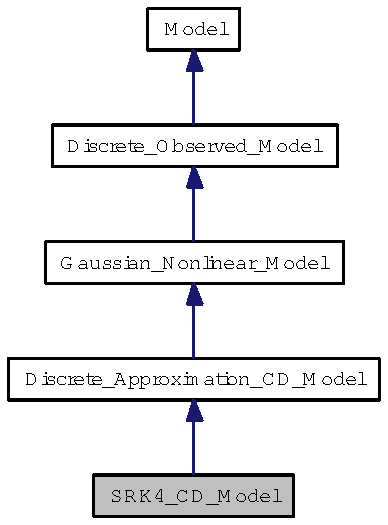
\includegraphics[width=111pt]{class_s_r_k4___c_d___model__inherit__graph}
\end{center}
\end{figure}
\subsection*{Public Member Functions}
\begin{CompactItemize}
\item 
\hyperlink{class_s_r_k4___c_d___model_52708f290c0dfb41c8de289c2e716cb3}{SRK4\_\-CD\_\-Model} (void)
\item 
\hyperlink{class_s_r_k4___c_d___model_e1ae17aa1fe147b7da45493f2d4db40c}{SRK4\_\-CD\_\-Model} (\hyperlink{class_continuous___discrete___model}{Continuous\_\-Discrete\_\-Model} $\ast$m, const int \&a)
\item 
dcovector \hyperlink{class_s_r_k4___c_d___model_553c1dc82fe1e497ff73a919e6bd98e6}{Scheme} (const dcovector \&X, const dcovector \&W)
\item 
void \hyperlink{class_s_r_k4___c_d___model_c348e8a59d0880ac366190004f4df36b}{Get\_\-Linear\_\-Scheme} (const dcovector \&X, const dcovector \&W, dgematrix \&F, dgematrix \&J, dcovector \&Xp)
\begin{CompactList}\small\item\em Get the Linearized parameters Scheme in X,W. \item\end{CompactList}\item 
dgematrix \hyperlink{class_s_r_k4___c_d___model_2e0543a20a7ba52958606bda265413bd}{Jx\_\-Scheme} (const dcovector \&X, const dcovector \&W)
\item 
dgematrix \hyperlink{class_s_r_k4___c_d___model_37045148c197b6143df008855179dfa3}{Jw\_\-Scheme} (const dcovector \&X, const dcovector \&W)
\end{CompactItemize}


\subsection{Detailed Description}
continuous discret model: the state SDE is discretly approximate by an Sstochastic runge kutta method 

\subsection{Constructor \& Destructor Documentation}
\hypertarget{class_s_r_k4___c_d___model_52708f290c0dfb41c8de289c2e716cb3}{
\index{SRK4\_\-CD\_\-Model@{SRK4\_\-CD\_\-Model}!SRK4\_\-CD\_\-Model@{SRK4\_\-CD\_\-Model}}
\index{SRK4\_\-CD\_\-Model@{SRK4\_\-CD\_\-Model}!SRK4_CD_Model@{SRK4\_\-CD\_\-Model}}
\subsubsection[{SRK4\_\-CD\_\-Model}]{\setlength{\rightskip}{0pt plus 5cm}SRK4\_\-CD\_\-Model::SRK4\_\-CD\_\-Model (void)}}
\label{class_s_r_k4___c_d___model_52708f290c0dfb41c8de289c2e716cb3}


\hypertarget{class_s_r_k4___c_d___model_e1ae17aa1fe147b7da45493f2d4db40c}{
\index{SRK4\_\-CD\_\-Model@{SRK4\_\-CD\_\-Model}!SRK4\_\-CD\_\-Model@{SRK4\_\-CD\_\-Model}}
\index{SRK4\_\-CD\_\-Model@{SRK4\_\-CD\_\-Model}!SRK4_CD_Model@{SRK4\_\-CD\_\-Model}}
\subsubsection[{SRK4\_\-CD\_\-Model}]{\setlength{\rightskip}{0pt plus 5cm}SRK4\_\-CD\_\-Model::SRK4\_\-CD\_\-Model ({\bf Continuous\_\-Discrete\_\-Model} $\ast$ {\em m}, \/  const int \& {\em a})}}
\label{class_s_r_k4___c_d___model_e1ae17aa1fe147b7da45493f2d4db40c}




\subsection{Member Function Documentation}
\hypertarget{class_s_r_k4___c_d___model_c348e8a59d0880ac366190004f4df36b}{
\index{SRK4\_\-CD\_\-Model@{SRK4\_\-CD\_\-Model}!Get\_\-Linear\_\-Scheme@{Get\_\-Linear\_\-Scheme}}
\index{Get\_\-Linear\_\-Scheme@{Get\_\-Linear\_\-Scheme}!SRK4_CD_Model@{SRK4\_\-CD\_\-Model}}
\subsubsection[{Get\_\-Linear\_\-Scheme}]{\setlength{\rightskip}{0pt plus 5cm}void SRK4\_\-CD\_\-Model::Get\_\-Linear\_\-Scheme (const dcovector \& {\em X}, \/  const dcovector \& {\em W}, \/  dgematrix \& {\em F}, \/  dgematrix \& {\em J}, \/  dcovector \& {\em Xp})\hspace{0.3cm}{\tt  \mbox{[}virtual\mbox{]}}}}
\label{class_s_r_k4___c_d___model_c348e8a59d0880ac366190004f4df36b}


Get the Linearized parameters Scheme in X,W. 

\begin{Desc}
\item[Parameters:]
\begin{description}
\item[{\em X}]The state value \item[{\em W}]The noise value \item[{\em F}]The jacobian of f(X,W) in X \item[{\em G}]The jacobian in f(X,W) in W \item[{\em Xp}]The prediction Xp = f(X,W) \end{description}
\end{Desc}


Implements \hyperlink{class_discrete___approximation___c_d___model_0a486fada10e6f5569d186edc7b32110}{Discrete\_\-Approximation\_\-CD\_\-Model}.\hypertarget{class_s_r_k4___c_d___model_37045148c197b6143df008855179dfa3}{
\index{SRK4\_\-CD\_\-Model@{SRK4\_\-CD\_\-Model}!Jw\_\-Scheme@{Jw\_\-Scheme}}
\index{Jw\_\-Scheme@{Jw\_\-Scheme}!SRK4_CD_Model@{SRK4\_\-CD\_\-Model}}
\subsubsection[{Jw\_\-Scheme}]{\setlength{\rightskip}{0pt plus 5cm}dgematrix SRK4\_\-CD\_\-Model::Jw\_\-Scheme (const dcovector \& {\em X}, \/  const dcovector \& {\em W})\hspace{0.3cm}{\tt  \mbox{[}virtual\mbox{]}}}}
\label{class_s_r_k4___c_d___model_37045148c197b6143df008855179dfa3}




Implements \hyperlink{class_discrete___approximation___c_d___model_c7496999409a3f05125ceb7fe85e85ab}{Discrete\_\-Approximation\_\-CD\_\-Model}.\hypertarget{class_s_r_k4___c_d___model_2e0543a20a7ba52958606bda265413bd}{
\index{SRK4\_\-CD\_\-Model@{SRK4\_\-CD\_\-Model}!Jx\_\-Scheme@{Jx\_\-Scheme}}
\index{Jx\_\-Scheme@{Jx\_\-Scheme}!SRK4_CD_Model@{SRK4\_\-CD\_\-Model}}
\subsubsection[{Jx\_\-Scheme}]{\setlength{\rightskip}{0pt plus 5cm}dgematrix SRK4\_\-CD\_\-Model::Jx\_\-Scheme (const dcovector \& {\em X}, \/  const dcovector \& {\em W})\hspace{0.3cm}{\tt  \mbox{[}virtual\mbox{]}}}}
\label{class_s_r_k4___c_d___model_2e0543a20a7ba52958606bda265413bd}




Implements \hyperlink{class_discrete___approximation___c_d___model_7a3dcae055d90be0b8a231eff961e2a2}{Discrete\_\-Approximation\_\-CD\_\-Model}.\hypertarget{class_s_r_k4___c_d___model_553c1dc82fe1e497ff73a919e6bd98e6}{
\index{SRK4\_\-CD\_\-Model@{SRK4\_\-CD\_\-Model}!Scheme@{Scheme}}
\index{Scheme@{Scheme}!SRK4_CD_Model@{SRK4\_\-CD\_\-Model}}
\subsubsection[{Scheme}]{\setlength{\rightskip}{0pt plus 5cm}dcovector SRK4\_\-CD\_\-Model::Scheme (const dcovector \& {\em X}, \/  const dcovector \& {\em W})\hspace{0.3cm}{\tt  \mbox{[}virtual\mbox{]}}}}
\label{class_s_r_k4___c_d___model_553c1dc82fe1e497ff73a919e6bd98e6}




Implements \hyperlink{class_discrete___approximation___c_d___model_1ea9a1d618890fc51db6fa98eeb7af7f}{Discrete\_\-Approximation\_\-CD\_\-Model}.
\hypertarget{class_t_h_g_l___filter}{
\section{THGL\_\-Filter Class Reference}
\label{class_t_h_g_l___filter}\index{THGL\_\-Filter@{THGL\_\-Filter}}
}
{\tt \#include $<$thgl\_\-filter.h$>$}

Inheritance diagram for THGL\_\-Filter:\nopagebreak
\begin{figure}[H]
\begin{center}
\leavevmode
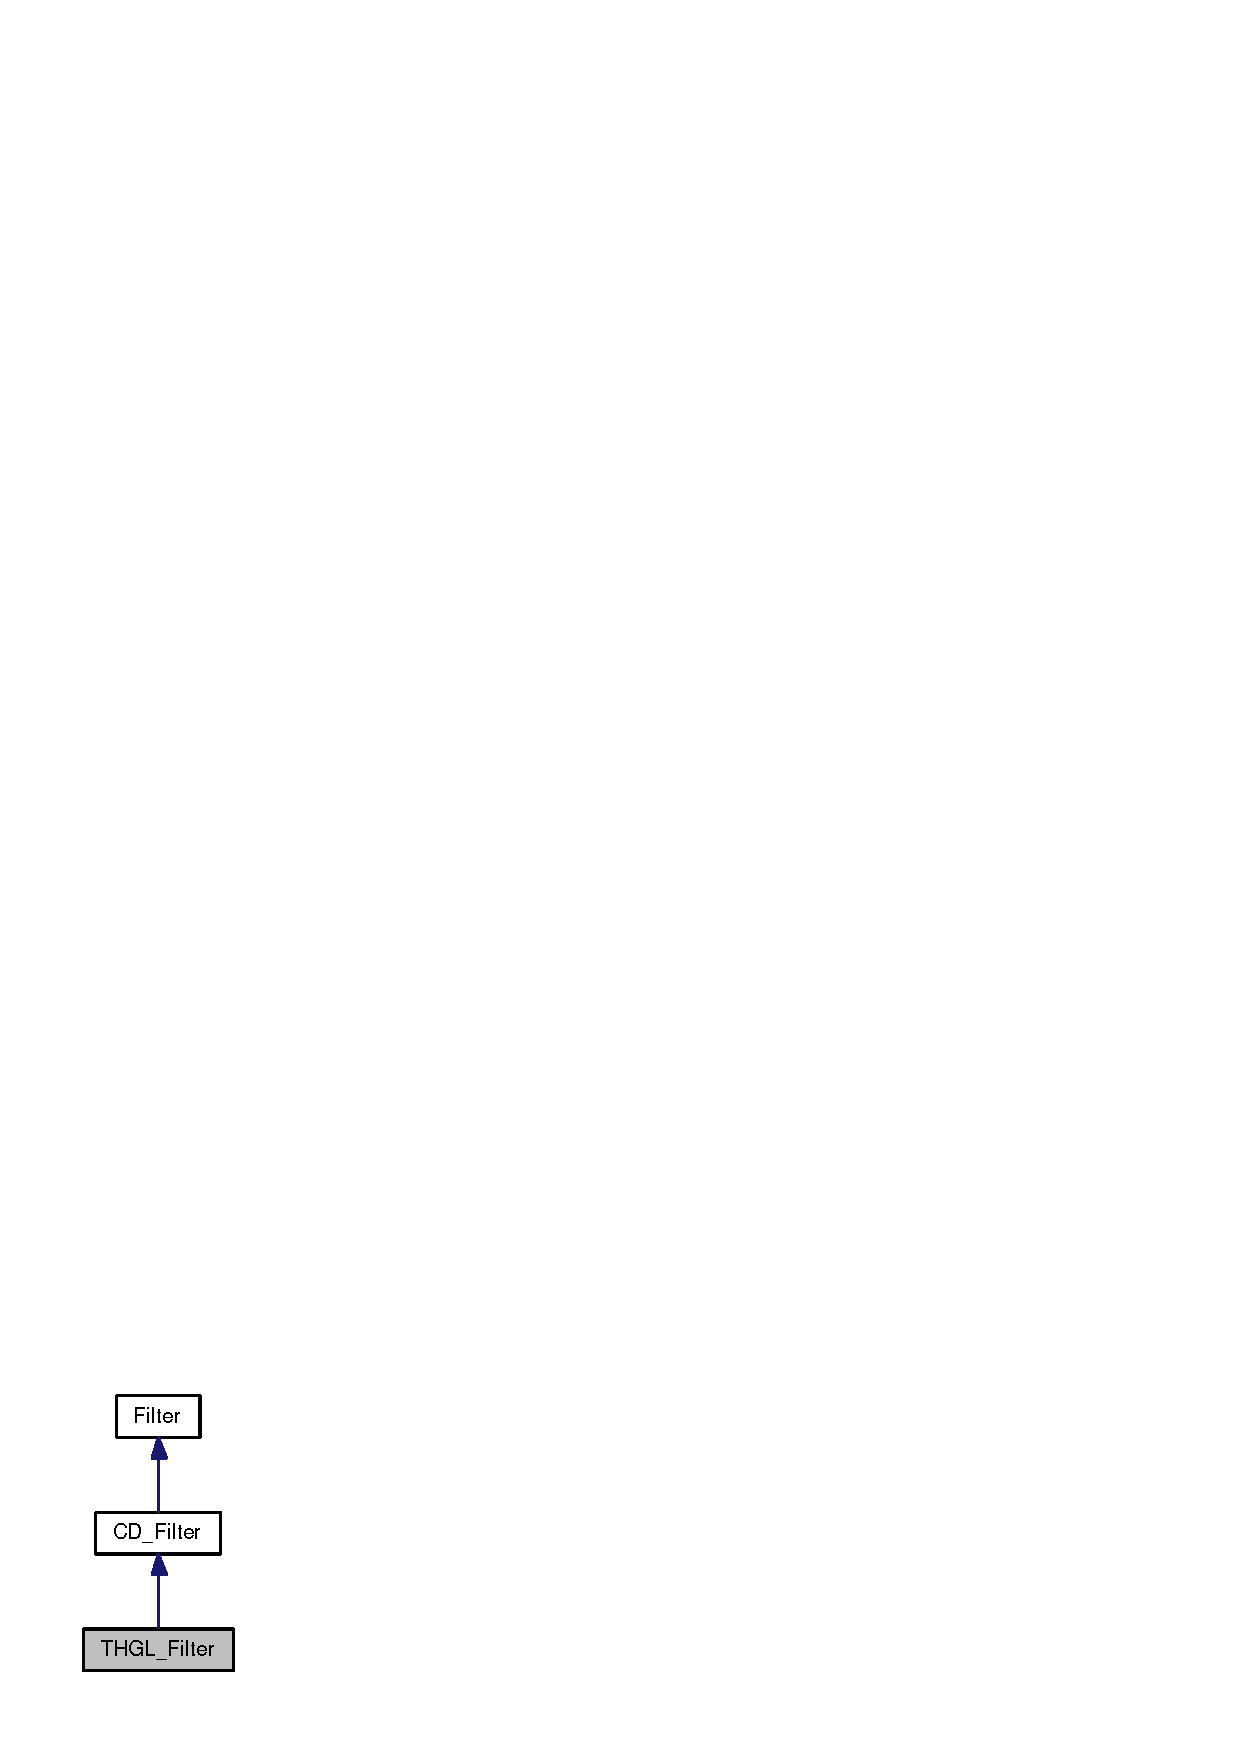
\includegraphics[width=58pt]{class_t_h_g_l___filter__inherit__graph}
\end{center}
\end{figure}
\subsection*{Public Member Functions}
\begin{CompactItemize}
\item 
\hyperlink{class_t_h_g_l___filter_4bd120e267d0de8863eebc154dd3730d}{THGL\_\-Filter} (void)
\item 
\hyperlink{class_t_h_g_l___filter_cd237359274fb7e0e7a7f00570acd76a}{THGL\_\-Filter} (\hyperlink{class_continuous___discrete___model}{Continuous\_\-Discrete\_\-Model} $\ast$m)
\end{CompactItemize}
\subsection*{Protected Member Functions}
\begin{CompactItemize}
\item 
int \hyperlink{class_t_h_g_l___filter_2139ff41dc0eaa613847429c266ba7a5}{\_\-update} (const dcovector \&Y)
\end{CompactItemize}


\subsection{Constructor \& Destructor Documentation}
\hypertarget{class_t_h_g_l___filter_4bd120e267d0de8863eebc154dd3730d}{
\index{THGL\_\-Filter@{THGL\_\-Filter}!THGL\_\-Filter@{THGL\_\-Filter}}
\index{THGL\_\-Filter@{THGL\_\-Filter}!THGL_Filter@{THGL\_\-Filter}}
\subsubsection[{THGL\_\-Filter}]{\setlength{\rightskip}{0pt plus 5cm}THGL\_\-Filter::THGL\_\-Filter (void)}}
\label{class_t_h_g_l___filter_4bd120e267d0de8863eebc154dd3730d}


\hypertarget{class_t_h_g_l___filter_cd237359274fb7e0e7a7f00570acd76a}{
\index{THGL\_\-Filter@{THGL\_\-Filter}!THGL\_\-Filter@{THGL\_\-Filter}}
\index{THGL\_\-Filter@{THGL\_\-Filter}!THGL_Filter@{THGL\_\-Filter}}
\subsubsection[{THGL\_\-Filter}]{\setlength{\rightskip}{0pt plus 5cm}THGL\_\-Filter::THGL\_\-Filter ({\bf Continuous\_\-Discrete\_\-Model} $\ast$ {\em m})}}
\label{class_t_h_g_l___filter_cd237359274fb7e0e7a7f00570acd76a}




\subsection{Member Function Documentation}
\hypertarget{class_t_h_g_l___filter_2139ff41dc0eaa613847429c266ba7a5}{
\index{THGL\_\-Filter@{THGL\_\-Filter}!\_\-update@{\_\-update}}
\index{\_\-update@{\_\-update}!THGL_Filter@{THGL\_\-Filter}}
\subsubsection[{\_\-update}]{\setlength{\rightskip}{0pt plus 5cm}int THGL\_\-Filter::\_\-update (const dcovector \& {\em Y})\hspace{0.3cm}{\tt  \mbox{[}protected, virtual\mbox{]}}}}
\label{class_t_h_g_l___filter_2139ff41dc0eaa613847429c266ba7a5}


Specific update for each filter

\begin{Desc}
\item[Parameters:]
\begin{description}
\item[{\em Y}]The observed sample\end{description}
\end{Desc}
\begin{Desc}
\item[Returns:]0 if no problem \end{Desc}


Implements \hyperlink{class_filter_20ecd17fed3b8f11a76c960fe5e7144b}{Filter}.
\hypertarget{class_unscented___kalman___filter}{
\section{Unscented\_\-Kalman\_\-Filter Class Reference}
\label{class_unscented___kalman___filter}\index{Unscented\_\-Kalman\_\-Filter@{Unscented\_\-Kalman\_\-Filter}}
}
The Discrete Unscented Kalman \hyperlink{class_filter}{Filter} (UKF).  


{\tt \#include $<$unscented\_\-kalman\_\-filter.h$>$}

Inheritance diagram for Unscented\_\-Kalman\_\-Filter:\nopagebreak
\begin{figure}[H]
\begin{center}
\leavevmode
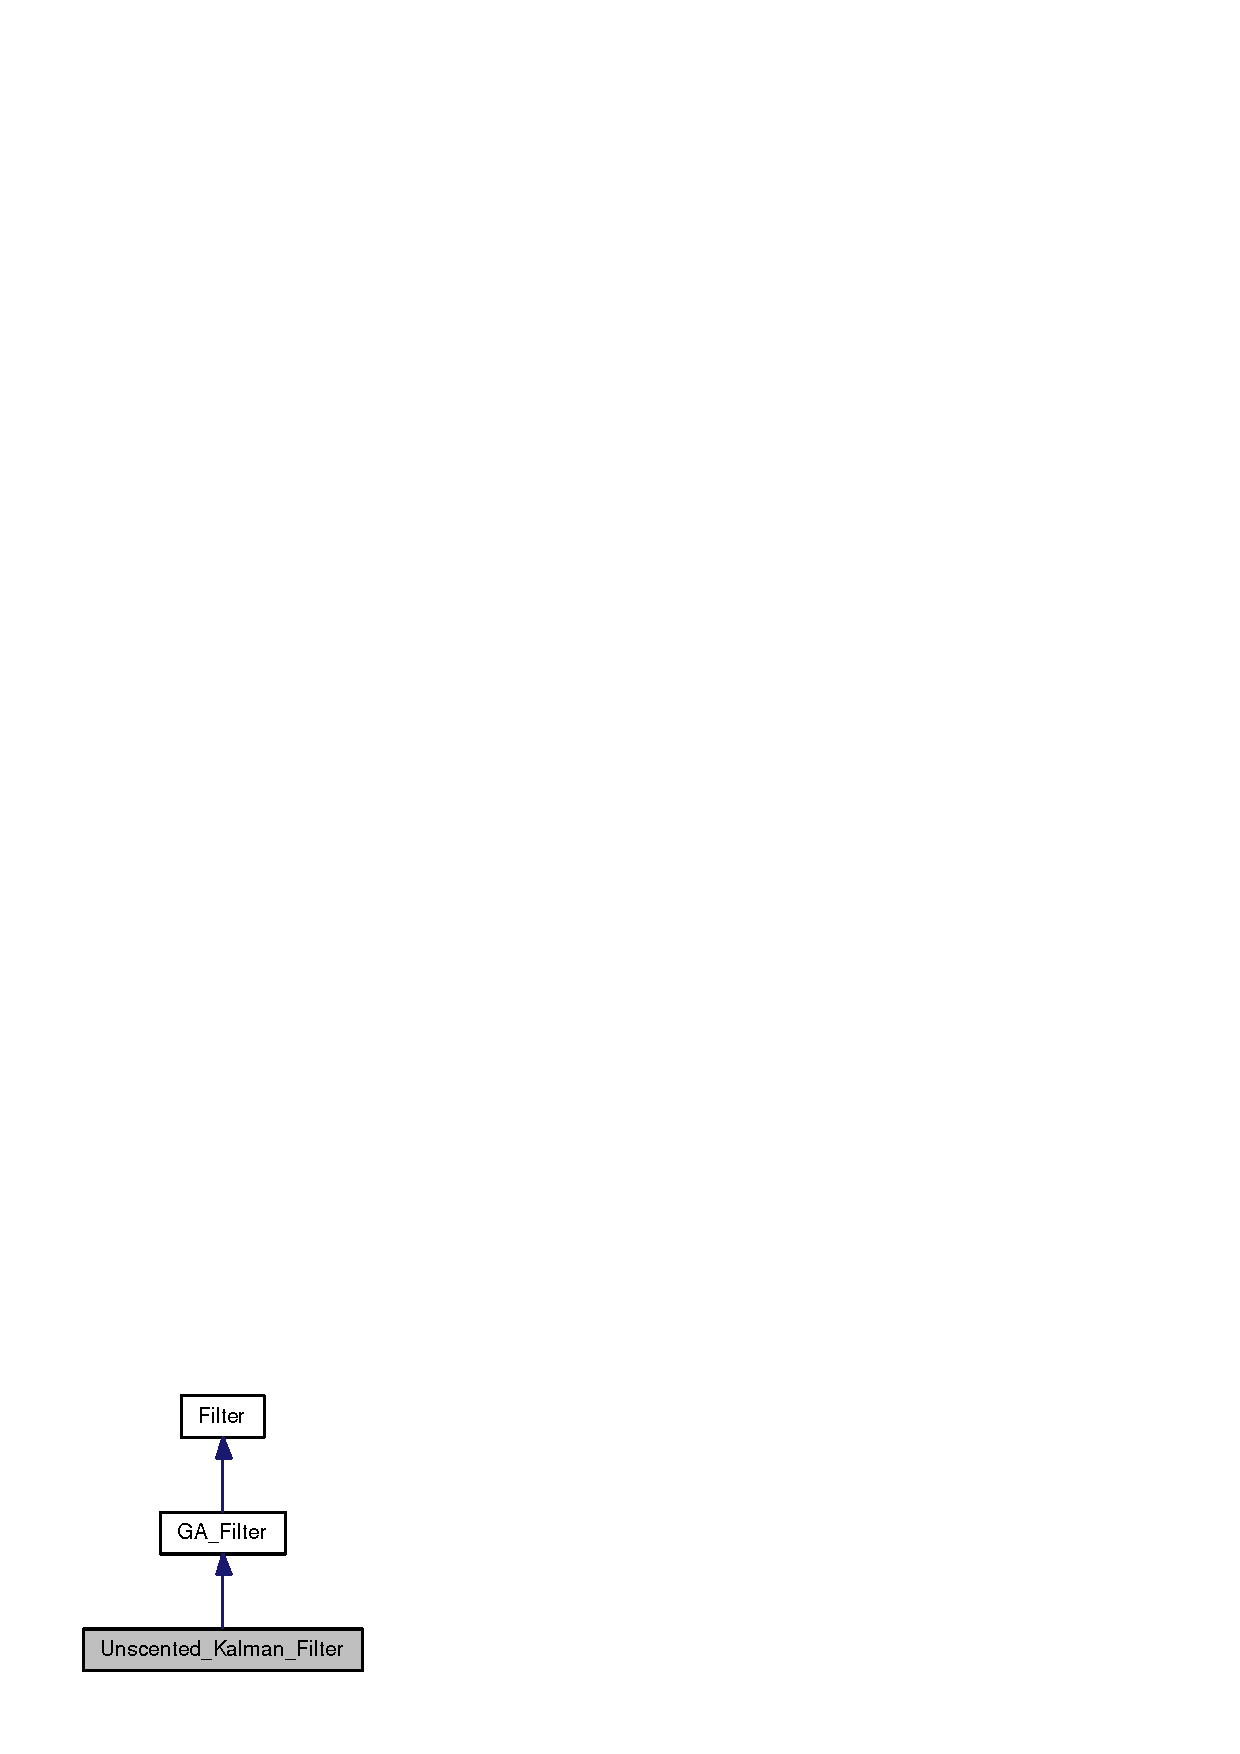
\includegraphics[width=89pt]{class_unscented___kalman___filter__inherit__graph}
\end{center}
\end{figure}
\subsection*{Public Member Functions}
\begin{CompactItemize}
\item 
\hyperlink{class_unscented___kalman___filter_9604c9cbd68ec0ba603964f2677c7e2e}{Unscented\_\-Kalman\_\-Filter} (void)
\begin{CompactList}\small\item\em A constructor. \item\end{CompactList}\item 
\hyperlink{class_unscented___kalman___filter_b1095ded70883e7a2389fd925fe1e378}{Unscented\_\-Kalman\_\-Filter} (\hyperlink{class_gaussian___nonlinear___model}{Gaussian\_\-Nonlinear\_\-Model} $\ast$\hyperlink{class_filter_2173d25727b871e9b9d0b6f588ba3cd2}{model})
\begin{CompactList}\small\item\em The constructor. \item\end{CompactList}\end{CompactItemize}
\subsection*{Public Attributes}
\begin{CompactItemize}
\item 
float \hyperlink{class_unscented___kalman___filter_a160d1820d77b547fee70f25747db2cb}{lambda}
\begin{CompactList}\small\item\em A scaled parameter. \item\end{CompactList}\end{CompactItemize}
\subsection*{Protected Member Functions}
\begin{CompactItemize}
\item 
int \hyperlink{class_unscented___kalman___filter_bbc48e2cfd73c0427cedea914e68ed1a}{SP\_\-Init} (void)
\begin{CompactList}\small\item\em Initialize the sigma points at each update step. \item\end{CompactList}\item 
int \hyperlink{class_unscented___kalman___filter_1229b08a8f97c4a877baedd390d0c55d}{U\_\-Cov} (const vector$<$ dcovector $>$ \&sP1, const dcovector \&m1, const vector$<$ dcovector $>$ \&sP2, const dcovector \&m2, dgematrix \&cov)
\begin{CompactList}\small\item\em Calculate the covaraince between two sets of sigma points. \item\end{CompactList}\item 
int \hyperlink{class_unscented___kalman___filter_5a6250da8fa76f0f5b22c9030e4ef157}{U\_\-Mean} (const vector$<$ dcovector $>$ \&sP, dcovector \&mean)
\begin{CompactList}\small\item\em Calculate the mean of a set of sigma points. \item\end{CompactList}\item 
int \hyperlink{class_unscented___kalman___filter_ee1e0a8035111d7695b6958c644f97cc}{\_\-update} (const dcovector \&Y)
\item 
int \hyperlink{class_unscented___kalman___filter_a6ca6d9f8b5a4a40c18b6cdfdc2029fa}{\_\-init} (void)
\begin{CompactList}\small\item\em Itialization of the UKF. \item\end{CompactList}\end{CompactItemize}
\subsection*{Private Attributes}
\begin{CompactItemize}
\item 
dgematrix \hyperlink{class_unscented___kalman___filter_ec03d2f57b006cad497c6bb30dae67c8}{sqrt\_\-Qw}
\begin{CompactList}\small\item\em The square root matrix (cholesky) of Qw. \item\end{CompactList}\item 
dgematrix \hyperlink{class_unscented___kalman___filter_633326bb2df6487da083ff8c7e09acdd}{sqrt\_\-Qv}
\begin{CompactList}\small\item\em The square root matrix (cholesky) of Qv. \item\end{CompactList}\item 
vector$<$ dcovector $>$ \hyperlink{class_unscented___kalman___filter_cd473b335bae84f2da4a18f412962127}{sX}
\begin{CompactList}\small\item\em The sigma points for the state X. \item\end{CompactList}\item 
vector$<$ dcovector $>$ \hyperlink{class_unscented___kalman___filter_3a77ce84c121d28608edd4a6f550aeae}{sW}
\begin{CompactList}\small\item\em The sigma points for the state noise W. \item\end{CompactList}\item 
vector$<$ dcovector $>$ \hyperlink{class_unscented___kalman___filter_4e7f5cd7580c525eb27c489dd5785453}{sY}
\begin{CompactList}\small\item\em The sigma points for the observation. \item\end{CompactList}\item 
double \hyperlink{class_unscented___kalman___filter_59707b0a7653a0610266e553eb5786f6}{w\_\-0}
\begin{CompactList}\small\item\em The first weight to compute the mean. \item\end{CompactList}\item 
double \hyperlink{class_unscented___kalman___filter_d04e96c03af71db29723963be6999be6}{w\_\-0c}
\begin{CompactList}\small\item\em The first weight to compute the covariance. \item\end{CompactList}\item 
double \hyperlink{class_unscented___kalman___filter_1869e471af5a12af031e9ff436756b95}{w}
\begin{CompactList}\small\item\em Other weights. \item\end{CompactList}\end{CompactItemize}


\subsection{Detailed Description}
The Discrete Unscented Kalman \hyperlink{class_filter}{Filter} (UKF). 



\subsection{Constructor \& Destructor Documentation}
\hypertarget{class_unscented___kalman___filter_9604c9cbd68ec0ba603964f2677c7e2e}{
\index{Unscented\_\-Kalman\_\-Filter@{Unscented\_\-Kalman\_\-Filter}!Unscented\_\-Kalman\_\-Filter@{Unscented\_\-Kalman\_\-Filter}}
\index{Unscented\_\-Kalman\_\-Filter@{Unscented\_\-Kalman\_\-Filter}!Unscented_Kalman_Filter@{Unscented\_\-Kalman\_\-Filter}}
\subsubsection[{Unscented\_\-Kalman\_\-Filter}]{\setlength{\rightskip}{0pt plus 5cm}Unscented\_\-Kalman\_\-Filter::Unscented\_\-Kalman\_\-Filter (void)}}
\label{class_unscented___kalman___filter_9604c9cbd68ec0ba603964f2677c7e2e}


A constructor. 

\hypertarget{class_unscented___kalman___filter_b1095ded70883e7a2389fd925fe1e378}{
\index{Unscented\_\-Kalman\_\-Filter@{Unscented\_\-Kalman\_\-Filter}!Unscented\_\-Kalman\_\-Filter@{Unscented\_\-Kalman\_\-Filter}}
\index{Unscented\_\-Kalman\_\-Filter@{Unscented\_\-Kalman\_\-Filter}!Unscented_Kalman_Filter@{Unscented\_\-Kalman\_\-Filter}}
\subsubsection[{Unscented\_\-Kalman\_\-Filter}]{\setlength{\rightskip}{0pt plus 5cm}Unscented\_\-Kalman\_\-Filter::Unscented\_\-Kalman\_\-Filter ({\bf Gaussian\_\-Nonlinear\_\-Model} $\ast$ {\em model})}}
\label{class_unscented___kalman___filter_b1095ded70883e7a2389fd925fe1e378}


The constructor. 

\begin{Desc}
\item[Parameters:]
\begin{description}
\item[{\em model}]A gaussian non linear model \end{description}
\end{Desc}


\subsection{Member Function Documentation}
\hypertarget{class_unscented___kalman___filter_a6ca6d9f8b5a4a40c18b6cdfdc2029fa}{
\index{Unscented\_\-Kalman\_\-Filter@{Unscented\_\-Kalman\_\-Filter}!\_\-init@{\_\-init}}
\index{\_\-init@{\_\-init}!Unscented_Kalman_Filter@{Unscented\_\-Kalman\_\-Filter}}
\subsubsection[{\_\-init}]{\setlength{\rightskip}{0pt plus 5cm}int Unscented\_\-Kalman\_\-Filter::\_\-init (void)\hspace{0.3cm}{\tt  \mbox{[}protected, virtual\mbox{]}}}}
\label{class_unscented___kalman___filter_a6ca6d9f8b5a4a40c18b6cdfdc2029fa}


Itialization of the UKF. 



Reimplemented from \hyperlink{class_g_a___filter_7b5cb872bcedd752a4309f114625a4b8}{GA\_\-Filter}.\hypertarget{class_unscented___kalman___filter_ee1e0a8035111d7695b6958c644f97cc}{
\index{Unscented\_\-Kalman\_\-Filter@{Unscented\_\-Kalman\_\-Filter}!\_\-update@{\_\-update}}
\index{\_\-update@{\_\-update}!Unscented_Kalman_Filter@{Unscented\_\-Kalman\_\-Filter}}
\subsubsection[{\_\-update}]{\setlength{\rightskip}{0pt plus 5cm}int Unscented\_\-Kalman\_\-Filter::\_\-update (const dcovector \& {\em Y})\hspace{0.3cm}{\tt  \mbox{[}protected, virtual\mbox{]}}}}
\label{class_unscented___kalman___filter_ee1e0a8035111d7695b6958c644f97cc}


Specific update for each filter

\begin{Desc}
\item[Parameters:]
\begin{description}
\item[{\em Y}]The observed sample\end{description}
\end{Desc}
\begin{Desc}
\item[Returns:]0 if no problem \end{Desc}


Implements \hyperlink{class_filter_20ecd17fed3b8f11a76c960fe5e7144b}{Filter}.\hypertarget{class_unscented___kalman___filter_bbc48e2cfd73c0427cedea914e68ed1a}{
\index{Unscented\_\-Kalman\_\-Filter@{Unscented\_\-Kalman\_\-Filter}!SP\_\-Init@{SP\_\-Init}}
\index{SP\_\-Init@{SP\_\-Init}!Unscented_Kalman_Filter@{Unscented\_\-Kalman\_\-Filter}}
\subsubsection[{SP\_\-Init}]{\setlength{\rightskip}{0pt plus 5cm}int Unscented\_\-Kalman\_\-Filter::SP\_\-Init (void)\hspace{0.3cm}{\tt  \mbox{[}protected\mbox{]}}}}
\label{class_unscented___kalman___filter_bbc48e2cfd73c0427cedea914e68ed1a}


Initialize the sigma points at each update step. 

\hypertarget{class_unscented___kalman___filter_1229b08a8f97c4a877baedd390d0c55d}{
\index{Unscented\_\-Kalman\_\-Filter@{Unscented\_\-Kalman\_\-Filter}!U\_\-Cov@{U\_\-Cov}}
\index{U\_\-Cov@{U\_\-Cov}!Unscented_Kalman_Filter@{Unscented\_\-Kalman\_\-Filter}}
\subsubsection[{U\_\-Cov}]{\setlength{\rightskip}{0pt plus 5cm}int Unscented\_\-Kalman\_\-Filter::U\_\-Cov (const vector$<$ dcovector $>$ \& {\em sP1}, \/  const dcovector \& {\em m1}, \/  const vector$<$ dcovector $>$ \& {\em sP2}, \/  const dcovector \& {\em m2}, \/  dgematrix \& {\em cov})\hspace{0.3cm}{\tt  \mbox{[}protected\mbox{]}}}}
\label{class_unscented___kalman___filter_1229b08a8f97c4a877baedd390d0c55d}


Calculate the covaraince between two sets of sigma points. 

\begin{Desc}
\item[Parameters:]
\begin{description}
\item[{\em sP1}]The first set of sigma point \item[{\em m1}]The mean of the sigma point \item[{\em sP2}]The second set of sigma point \item[{\em m2}]The mean of the second set of sigma point \item[{\em cov}]Return the empirical covariance matrix between two sets\end{description}
\end{Desc}
\begin{Desc}
\item[Returns:]0 if dimensions are ok \end{Desc}
\hypertarget{class_unscented___kalman___filter_5a6250da8fa76f0f5b22c9030e4ef157}{
\index{Unscented\_\-Kalman\_\-Filter@{Unscented\_\-Kalman\_\-Filter}!U\_\-Mean@{U\_\-Mean}}
\index{U\_\-Mean@{U\_\-Mean}!Unscented_Kalman_Filter@{Unscented\_\-Kalman\_\-Filter}}
\subsubsection[{U\_\-Mean}]{\setlength{\rightskip}{0pt plus 5cm}int Unscented\_\-Kalman\_\-Filter::U\_\-Mean (const vector$<$ dcovector $>$ \& {\em sP}, \/  dcovector \& {\em mean})\hspace{0.3cm}{\tt  \mbox{[}protected\mbox{]}}}}
\label{class_unscented___kalman___filter_5a6250da8fa76f0f5b22c9030e4ef157}


Calculate the mean of a set of sigma points. 

\begin{Desc}
\item[Parameters:]
\begin{description}
\item[{\em sP}]a set of sigma point \item[{\em mean}]Return the mean\end{description}
\end{Desc}
\begin{Desc}
\item[Returns:]0 if dimensions are ok \end{Desc}


\subsection{Member Data Documentation}
\hypertarget{class_unscented___kalman___filter_a160d1820d77b547fee70f25747db2cb}{
\index{Unscented\_\-Kalman\_\-Filter@{Unscented\_\-Kalman\_\-Filter}!lambda@{lambda}}
\index{lambda@{lambda}!Unscented_Kalman_Filter@{Unscented\_\-Kalman\_\-Filter}}
\subsubsection[{lambda}]{\setlength{\rightskip}{0pt plus 5cm}float {\bf Unscented\_\-Kalman\_\-Filter::lambda}}}
\label{class_unscented___kalman___filter_a160d1820d77b547fee70f25747db2cb}


A scaled parameter. 

\hypertarget{class_unscented___kalman___filter_633326bb2df6487da083ff8c7e09acdd}{
\index{Unscented\_\-Kalman\_\-Filter@{Unscented\_\-Kalman\_\-Filter}!sqrt\_\-Qv@{sqrt\_\-Qv}}
\index{sqrt\_\-Qv@{sqrt\_\-Qv}!Unscented_Kalman_Filter@{Unscented\_\-Kalman\_\-Filter}}
\subsubsection[{sqrt\_\-Qv}]{\setlength{\rightskip}{0pt plus 5cm}dgematrix {\bf Unscented\_\-Kalman\_\-Filter::sqrt\_\-Qv}\hspace{0.3cm}{\tt  \mbox{[}private\mbox{]}}}}
\label{class_unscented___kalman___filter_633326bb2df6487da083ff8c7e09acdd}


The square root matrix (cholesky) of Qv. 

\hypertarget{class_unscented___kalman___filter_ec03d2f57b006cad497c6bb30dae67c8}{
\index{Unscented\_\-Kalman\_\-Filter@{Unscented\_\-Kalman\_\-Filter}!sqrt\_\-Qw@{sqrt\_\-Qw}}
\index{sqrt\_\-Qw@{sqrt\_\-Qw}!Unscented_Kalman_Filter@{Unscented\_\-Kalman\_\-Filter}}
\subsubsection[{sqrt\_\-Qw}]{\setlength{\rightskip}{0pt plus 5cm}dgematrix {\bf Unscented\_\-Kalman\_\-Filter::sqrt\_\-Qw}\hspace{0.3cm}{\tt  \mbox{[}private\mbox{]}}}}
\label{class_unscented___kalman___filter_ec03d2f57b006cad497c6bb30dae67c8}


The square root matrix (cholesky) of Qw. 

\hypertarget{class_unscented___kalman___filter_3a77ce84c121d28608edd4a6f550aeae}{
\index{Unscented\_\-Kalman\_\-Filter@{Unscented\_\-Kalman\_\-Filter}!sW@{sW}}
\index{sW@{sW}!Unscented_Kalman_Filter@{Unscented\_\-Kalman\_\-Filter}}
\subsubsection[{sW}]{\setlength{\rightskip}{0pt plus 5cm}vector$<$dcovector$>$ {\bf Unscented\_\-Kalman\_\-Filter::sW}\hspace{0.3cm}{\tt  \mbox{[}private\mbox{]}}}}
\label{class_unscented___kalman___filter_3a77ce84c121d28608edd4a6f550aeae}


The sigma points for the state noise W. 

\hypertarget{class_unscented___kalman___filter_cd473b335bae84f2da4a18f412962127}{
\index{Unscented\_\-Kalman\_\-Filter@{Unscented\_\-Kalman\_\-Filter}!sX@{sX}}
\index{sX@{sX}!Unscented_Kalman_Filter@{Unscented\_\-Kalman\_\-Filter}}
\subsubsection[{sX}]{\setlength{\rightskip}{0pt plus 5cm}vector$<$dcovector$>$ {\bf Unscented\_\-Kalman\_\-Filter::sX}\hspace{0.3cm}{\tt  \mbox{[}private\mbox{]}}}}
\label{class_unscented___kalman___filter_cd473b335bae84f2da4a18f412962127}


The sigma points for the state X. 

\hypertarget{class_unscented___kalman___filter_4e7f5cd7580c525eb27c489dd5785453}{
\index{Unscented\_\-Kalman\_\-Filter@{Unscented\_\-Kalman\_\-Filter}!sY@{sY}}
\index{sY@{sY}!Unscented_Kalman_Filter@{Unscented\_\-Kalman\_\-Filter}}
\subsubsection[{sY}]{\setlength{\rightskip}{0pt plus 5cm}vector$<$dcovector$>$ {\bf Unscented\_\-Kalman\_\-Filter::sY}\hspace{0.3cm}{\tt  \mbox{[}private\mbox{]}}}}
\label{class_unscented___kalman___filter_4e7f5cd7580c525eb27c489dd5785453}


The sigma points for the observation. 

\hypertarget{class_unscented___kalman___filter_1869e471af5a12af031e9ff436756b95}{
\index{Unscented\_\-Kalman\_\-Filter@{Unscented\_\-Kalman\_\-Filter}!w@{w}}
\index{w@{w}!Unscented_Kalman_Filter@{Unscented\_\-Kalman\_\-Filter}}
\subsubsection[{w}]{\setlength{\rightskip}{0pt plus 5cm}double {\bf Unscented\_\-Kalman\_\-Filter::w}\hspace{0.3cm}{\tt  \mbox{[}private\mbox{]}}}}
\label{class_unscented___kalman___filter_1869e471af5a12af031e9ff436756b95}


Other weights. 

\hypertarget{class_unscented___kalman___filter_59707b0a7653a0610266e553eb5786f6}{
\index{Unscented\_\-Kalman\_\-Filter@{Unscented\_\-Kalman\_\-Filter}!w\_\-0@{w\_\-0}}
\index{w\_\-0@{w\_\-0}!Unscented_Kalman_Filter@{Unscented\_\-Kalman\_\-Filter}}
\subsubsection[{w\_\-0}]{\setlength{\rightskip}{0pt plus 5cm}double {\bf Unscented\_\-Kalman\_\-Filter::w\_\-0}\hspace{0.3cm}{\tt  \mbox{[}private\mbox{]}}}}
\label{class_unscented___kalman___filter_59707b0a7653a0610266e553eb5786f6}


The first weight to compute the mean. 

\hypertarget{class_unscented___kalman___filter_d04e96c03af71db29723963be6999be6}{
\index{Unscented\_\-Kalman\_\-Filter@{Unscented\_\-Kalman\_\-Filter}!w\_\-0c@{w\_\-0c}}
\index{w\_\-0c@{w\_\-0c}!Unscented_Kalman_Filter@{Unscented\_\-Kalman\_\-Filter}}
\subsubsection[{w\_\-0c}]{\setlength{\rightskip}{0pt plus 5cm}double {\bf Unscented\_\-Kalman\_\-Filter::w\_\-0c}\hspace{0.3cm}{\tt  \mbox{[}private\mbox{]}}}}
\label{class_unscented___kalman___filter_d04e96c03af71db29723963be6999be6}


The first weight to compute the covariance. 


\hypertarget{class_weighted___sample}{
\section{Weighted\_\-Sample Class Reference}
\label{class_weighted___sample}\index{Weighted\_\-Sample@{Weighted\_\-Sample}}
}
{\tt \#include $<$sisr\_\-filter.h$>$}

\subsection*{Public Attributes}
\begin{CompactItemize}
\item 
dcovector \hyperlink{class_weighted___sample_e6c7d5be67327a3f46da6e62e5602203}{Value}
\begin{CompactList}\small\item\em The position. \item\end{CompactList}\item 
long double \hyperlink{class_weighted___sample_cabb8bc4261a082d4b87a202f5e30a7b}{Weight}
\begin{CompactList}\small\item\em The weight of the sample. \item\end{CompactList}\end{CompactItemize}


\subsection{Member Data Documentation}
\hypertarget{class_weighted___sample_e6c7d5be67327a3f46da6e62e5602203}{
\index{Weighted\_\-Sample@{Weighted\_\-Sample}!Value@{Value}}
\index{Value@{Value}!Weighted_Sample@{Weighted\_\-Sample}}
\subsubsection[{Value}]{\setlength{\rightskip}{0pt plus 5cm}dcovector {\bf Weighted\_\-Sample::Value}}}
\label{class_weighted___sample_e6c7d5be67327a3f46da6e62e5602203}


The position. 

\hypertarget{class_weighted___sample_cabb8bc4261a082d4b87a202f5e30a7b}{
\index{Weighted\_\-Sample@{Weighted\_\-Sample}!Weight@{Weight}}
\index{Weight@{Weight}!Weighted_Sample@{Weighted\_\-Sample}}
\subsubsection[{Weight}]{\setlength{\rightskip}{0pt plus 5cm}long double {\bf Weighted\_\-Sample::Weight}}}
\label{class_weighted___sample_cabb8bc4261a082d4b87a202f5e30a7b}


The weight of the sample. 


\printindex
\end{document}
